\documentclass[inscr,ack,preface]{diphdthesis}

%%%--------------------------------------------------------------
%%  Package Dependencies
%%%--------------------------------------------------------------

\usepackage[chapter]{algorithm}
\usepackage{algorithmicx}
\usepackage{algpseudocode}
\usepackage{alltt}
\usepackage{bookmark}
\usepackage{booktabs}
\usepackage{color,soul}
\usepackage{comment}
\usepackage{fancyhdr}
\usepackage{footnote}
\usepackage{graphicx}
\usepackage{marvosym}
\usepackage{multirow}
\usepackage{multicol}
\usepackage{mathtools}
\usepackage{epigraph}
\usepackage[defblank]{paralist}
% \usepackage{boxedminipage}
% \usepackage{varwidth}
\usepackage{url}
\usepackage{subcaption}
% \usepackage{cite}
% \captionsetup{compatibility=false}
\usepackage{verbatimbox}
\usepackage{minted}
\usemintedstyle{friendly}             % set minted colour theme
\usepackage{xparse}
\usepackage{hyperref}
\hypersetup{
    unicode=true,                     % non-Latin characters in bookmarks
    pdffitwindow=true,                % page fit to window when opened
    pdfnewwindow=true,                % links in new window
    pdfkeywords={},                   % list of keywords
    colorlinks=true,                  % false: boxed links; true: colored links
    linkcolor=black,                  % color of internal links
    citecolor=black,                  % color of links to bibliography
    filecolor=black,                  % color of file links
    urlcolor=black,                   % color of external links
    pdftitle={},                      % title
    pdfauthor={},                     % author
    pdfsubject={}                     % subject of the document
}

\input{revision}

% Additional Local packages
\usepackage{styles/mathpartir}

% For footnotes inside tabular environment. See footnote package
\makesavenoteenv{tabular}

%%%--------------------------------------------------------------
%%  Bibliography Management and Resources
%%%--------------------------------------------------------------

\usepackage[backend=bibtex,bibencoding=ascii,style=numeric-comp]{biblatex}
\addbibresource{bib/my-publications.bib}
\addbibresource{bib/thesis.bib}
\addbibresource{bib/class-hier-comp.bib}
\addbibresource{bib/reflection.bib}
\addbibresource{bib/ptr-analysis/ptranalysis.bib}
\addbibresource{bib/ptr-analysis/specs.bib}
\addbibresource{bib/ptr-analysis/tools.bib}
\addbibresource{bib/ptr-analysis/proceedings.bib}

\DeclareFieldFormat{titlecase}{\MakeSentenceCase{#1}}

%%%%%%%%%%%%%%%%%%%%%%%%%%%%%%%%%%%%%%%%%%%%%%%%%%%%%%%%%%%%%%%%%%%%%%%%%%%%%%%
%%%%%%%%%%%%%%%%%%%%%% User-specific configuration %%%%%%%%%%%%%%%%%%%%%%%%%%%%
%%%%%%%%%%%%%%%%%%%%%%%%%%%%%%%%%%%%%%%%%%%%%%%%%%%%%%%%%%%%%%%%%%%%%%%%%%%%%%%

\newcommand{\doop}{\textsc{Doop}}

\newcommand{\cclyzer}{\texttt{cclyzer}}
\newcommand{\pearce}{\emph{Pearce$^c$}}
\newcommand{\code}[1]{\texttt{#1}}
\newcommand{\pt}[1]{\texttt{\textsc{Pt}(#1)}}
\newcommand{\javaclass}[1]{\url{#1}}
\newcommand{\javamethod}[1]{\url{#1}}
\newcommand{\javasignature}[1]{\url{#1}}

\usepackage{styles/instructions}
\usepackage{styles/languages}
\usepackage{styles/mathmisc}
\usepackage{styles/algorithms}

% Separation logic operators
\newcommand{\sep}{-\kern-.6em\raisebox{-.659ex}{*}\ }

% Additional math operators
\newcommand{\dotrel}[1]{\mathrel{\dot{#1}}}
\newcommand{\simless}{\dotrel{\sim}}


%%%%%%%%%%%%%%%%%%%%%%%%%%%%%%%%%%%%%%%%%%%%%%%%%%%%%%%%%%%%%%%%%%%%%%%%%%%%%%%
%%%%%%%%%%%%%%%%%%%%%%%%%%% Required Metadata %%%%%%%%%%%%%%%%%%%%%%%%%%%%%%%%%
%%%%%%%%%%%%%%%%%%%%%%%%%%%%%%%%%%%%%%%%%%%%%%%%%%%%%%%%%%%%%%%%%%%%%%%%%%%%%%%
%
% First name, last name
%
\authorFirstGr{Γεώργιος}
\authorFirstAbrGr{Γ.} % abbreviation of first name
\authorMiddleGr{Δ.}   % abbreviation of father's first name
\authorLastGr{Μπαλατσούρας}
\authorFirstEn{George}
\authorFirstAbrEn{G.}
\authorMiddleEn{D.}
\authorLastEn{Balatsouras}

%
% The title of the thesis
%
\titleGr{Ανάκτηση Δομικής Πληροφορίας προς Καλύτερη Στατική Ανάλυση}
\titleEn{Recovering Structural Information for Better Static Analysis}

%
% Month followed by Year
%
\dateGr{ΑΠΡΙΛΙΟΣ 2017}
\dateEn{APRIL 2017}

%
% Advisor info
%
\advisorGr{Γιάννης Σμαραγδάκης}
\advisorRankGr{Καθηγητής}
\advisorOrgGr{ΕΚΠΑ}
\advisorEn{Yannis Smaragdakis}
\advisorRankEn{Professor}
\advisorOrgEn{NKUA}

%
% Members of the advisory board 
% (the first one, will be automatically taken up by the advisor)
%
\boardTwoGr{Αλέξης Δελής}
\boardTwoRankGr{Καθηγητής}
\boardTwoOrgGr{ΕΚΠΑ}
\boardTwoEn{Alex Delis}
\boardTwoRankEn{Professor}
\boardTwoOrgEn{NKUA}

\boardThreeGr{Παναγιώτης Ροντογιάννης}
\boardThreeRankGr{Καθηγητής}
\boardThreeOrgGr{ΕΚΠΑ}
\boardThreeEn{Panos Rondogiannis}
\boardThreeRankEn{Professor}
\boardThreeOrgEn{NKUA}

%
% 7 Member examination committee
% (the first three will be taken up by the advisory board)
%
\examFourGr{Μέμα Ρουσσοπούλου}
\examFourRankGr{Αναπληρώτρια Καθηγήτρια}
\examFourOrgGr{ΕΚΠΑ}
\examFourEn{Mema Roussopoulos}
\examFourRankEn{Associate Professor}
\examFourOrgEn{NKUA}

\examFiveGr{Μανόλης Κουμπαράκης}
\examFiveRankGr{Καθηγητής}
\examFiveOrgGr{ΕΚΠΑ}
\examFiveEn{Manolis Koubarakis}
\examFiveRankEn{Professor}
\examFiveOrgEn{NKUA}

\examSixGr{Νικόλαος Παπασπύρου}
\examSixRankGr{Αναπληρωτής Καθηγητής}
\examSixOrgGr{ΕΜΠ}
\examSixEn{Nikolaos Papaspyrou}
\examSixRankEn{Associate Professor}
\examSixOrgEn{NTUA}

\examSevenGr{Κωνσταντίνος Σαγώνας}
\examSevenRankGr{Αναπληρωτής Καθηγητής}
\examSevenOrgGr{ΕΜΠ}
\examSevenEn{Konstantinos Sagonas}
\examSevenRankEn{Associate Professor}
\examSevenOrgEn{NTUA}

%
% The examination date of the thesis
%
\examinationDateGr{2 Μαΐου 2017}
\examinationDateEn{May 2, 2017}

%
% Abstract, synopsis, inscription, ack, and preface pages.
%
\abstractEn{%%% Abstract in English

Static analysis aims to achieve a deep understanding of program
behavior, by automatic reasoning that requires only the program's
source code and not any actual execution. To reach a truly deep level
of program understanding, static analysis techniques need to create an
abstraction of memory that covers all possible executions. Such
abstract models may quickly degenerate after losing essential
structural information about the memory objects they describe, due to
the use of specific programming idioms and language features, or
because of practical analysis limitations. In many cases, some of the
lost memory structure may be retrieved, though it requires complex
inference that takes advantage of indirect uses of types. Such
recovered structural information may greatly benefit static analysis.

%%% Local Variables:
%%% mode: latex
%%% TeX-master: "thesis"
%%% End:
}
\abstractGr{%%% Abstract in Greek

Η στατική ανάλυση στοχεύει στην κατανόηση της συμπεριφοράς του
προγράμματος, μέσω αυτοματοποιημένων τεχνικών συμπερασμού βασιζόμενες
καθαρά στον πηγαίο κώδικα του προγράμματος, αλλά δίχως να προϋποθέτουν
την εκτέλεση του κώδικα αυτού. Για να πετύχουν αυτές οι τεχνικές μία
ευρεία κατανόηση του κώδικα, καταφεύγουν στη δημιουργία ενός
αφηρημένου μοντέλου της μνήμης, το οποίο καλύπτει όλες τις πιθανές
εκτελέσεις. Αφηρημένα μοντέλα τέτοιου τύπου μπορεί γρήγορα να
εκφυλιστούν, αν χάσουν σημαντική δομική πληροφορία των αντικειμένων
στη μνήμη που περιγράφουν. Αυτό συνήθως συμβαίνει λόγω χρήσης
συγκεκριμένων προγραμματιστικών ιδιωμάτων και χαρακτηριστικών της
γλώσσας προγραμματισμού, ή λόγω πρακτικών περιορισμών της ανάλυσης.
Σε αρκετές περιπτώσεις, ένα σημαντικό μέρος της χαμένης αυτής δομικής
πληροφορίας μπορεί να ανακτηθεί μέσω σύνθετης λογικής η οποία
παρακολουθεί την έμμεση χρήση τύπων και να χρησιμοποιηθεί προς όφελος
της στατικής ανάλυσης του προγράμματος αυτού.

Στη διατριβή αυτή παρουσιάζουμε διάφορους τρόπους ανάκτησης δομικής
πληροφορίας, πρώτα
\begin{inparaenum}[(1)]
\item σε προγράμματα {\en C/C++}, κι έπειτα, σε προγράμματα γλωσσών
  υψηλότερου επιπέδου που δεν προσφέρουν άμεση πρόσβαση μνήμης, όπως η
  {\en Java}, όπου αναγνωρίζουμε δύο βασικές πηγές απώλειας δομικής
  πληροφορίας:
\item χρήση ανάκλασης και
\item ανάλυση μερικών προγραμμάτων.
\end{inparaenum}
Δείχνουμε πως, σε όλες τις παραπάνω περιπτώσεις, η ανάκτηση τέτοιας
δομικής πληροφορίας βελτιώνει άμεσα τη στατική ανάλυση του
προγράμματος.

Παρουσιάζουμε μία ανάλυση δεικτών για {\en C/C++}, η οποία βελτιώνει
το επίπεδο της αφαίρεσης, βασιζόμενη σε πληροφορία τύπου που
ανακαλύπτει κατά τη διάρκεια της ανάλυσης. Παρέχουμε μία υλοποίηση της
ανάλυσης αυτής, στο {\en \cclyzer{}}, ένα εργαλείο στατικής ανάλυσης
για {\en LLVM bitcode}.
%
Έπειτα, παρουσιάζουμε επεκτάσεις σε ανάλυση δεικτών για {\en Java},
κτίζοντας πάνω σε σύγχρονες τεχνικές χειρισμού μηχανισμών ανάκλασης. Η
βασική αρχή είναι παραπλήσια με την περίπτωση της {\en C/C++}:
καταγράφουμε τη χρήση των ανακλαστικών αντικειμένων, κατά τη διάρκεια
της ανάλυσης δεικτών, ώστε να ανακαλύψουμε βασικά δομικά τους
στοιχεία, τα οποία μπορούμε να χρησιμοποιήσουμε έπειτα για να
βελτιώσουμε τον χειρισμό των εντολών ανάκλασης στην τρέχουσα ανάλυση,
με αμοιβαία αναδρομικό τρόπο.
%
Τέλος, ως προς την ανάλυση μερικών προγραμμάτων {\en Java}, ορίζουμε
το γενικό πρόβλημα της ((\emph{συμπλήρωσης προγράμματος})): δοθέντος
ενός μερικού προγράμματος, πως να εφεύρουμε ένα υποκατάστατο του
κώδικα που λείπει, έτσι ώστε αυτό να ικανοποιεί τους περιορισμούς των
στατικών και δυναμικών τύπων που υπονοούνται από τον υπάρχοντα
κώδικα. Ή διαφορετικά, πως να ανακτήσουμε τη δομή των τύπων που
λείπουν. Πέρα της ανακάλυψης των μελών (πεδίων και μεθόδων) των
κλάσεων που λείπουν, η ικανοποίηση των περιορισμών υποτυπισμού μας
οδηγεί στον ορισμό ενός πρωτότυπου προβλήματος τύπων στον
αντικειμενοστρεφή κόσμο: η συμπλήρωση ιεραρχίας τύπων. Παρέχουμε
αλγορίθμους που λύσουν το πρόβλημα αυτό σε διάφορα είδη
κληρονομικότητας (μονής, πολλαπλής, μεικτής) και τους υλοποιούμε στο
{\en JPhantom}, ένα νέο εργαλείο συμπλήρωσης {\en Java bytecode}
κώδικα.

%%% Local Variables:
%%% mode: latex
%%% TeX-master: "thesis"
%%% End:
}
\synopsisGr{Συνοπτική περιγραφή του διδακτορικού (5--8 σελίδες).}
\acksEn{
}
\prefaceEn{}

\inscriptionEn{\emph{To my dear person.}}

%
% Subject area and keywords
%
\subjectAreaGr{Γλώσσες Προγραμματισμού, Στατική Ανάλυση}
\subjectAreaEn{Programming Languages, Static Analysis}
\keywordsGr{Ανάλυση Δεικτών, Αντικειμενοστρεφής Προγραμματισμός, %
  Ιεραρχία Τύπων, Ανάκλαση}
\keywordsEn{Pointer Analysis; Object-Oriented Programming; Type %
  Hierarchy; Reflection}

% From Class Hierarchy Complementation paper
% \terms{Algorithms, Languages, Performance}
% \keywords{type hierarchy; Java; single inheritance; multiple
%   inheritance; JPhantom; bytecode engineering}

%
% Set the .bib file containing your paper publications (leave the extension out)
%
% This is optional, but it should be specified when option 'lop' is passed to
% the document class.
%
% Then, inside the document environment, you may use the command '\nocitelop' to
% cite your papers, as you would traditionally do with the commands '\cite' or
% '\nocite'.
%
% The papers are printed in reverse chronological order.
%
%\lopfile{mypapers/pubs}


\begin{document}

%%%%%%%%%%%%%%%%%%%%%%%%%%%%%%%%%%%%%%%%%%%%%%%%%%%%%%%%%%%%%%%%%%%%%%%%%%%%%%%%
%%%%%%%%%%%%%%%%%%%%%%%%%%%%%%%  Front Matter  %%%%%%%%%%%%%%%%%%%%%%%%%%%%%%%%%
%%%%%%%%%%%%%%%%%%%%%%%%%%%%%%%%%%%%%%%%%%%%%%%%%%%%%%%%%%%%%%%%%%%%%%%%%%%%%%%%

\frontmatter

% cite my papers
%\nocitelop{}

%%%%%%%%%%%%%%%%%%%%%%%%%%%%%%%%%%%%%%%%%%%%%%%%%%%%%%%%%%%%%%%%%%%%%%%%%%%%%%%%
%%%%%%%%%%%%%%%%%%%%%%%%%%%%%%%   Main Matter  %%%%%%%%%%%%%%%%%%%%%%%%%%%%%%%%%
%%%%%%%%%%%%%%%%%%%%%%%%%%%%%%%%%%%%%%%%%%%%%%%%%%%%%%%%%%%%%%%%%%%%%%%%%%%%%%%%

\mainmatter

% add main chapters (should be given in capital letters)
\chapter{Introduction}
Static program analysis is a vast field with broad uses; an umbrella
term for many different methodologies (%
\begin{inparablank}
  \item Hoare logic
    \cite{journals/cacm/Hoare69,floyd1967assigning,lics:2002/Reynolds,csl/OHearnRY01},
  \item model checking
    \cite{icalp/EmersonC80,lop/ClarkeE81,toplas/ClarkeES86,programm/QueilleS82},
  \item symbolic execution
    \cite{journals/cacm/King76,journals/tse/Howden77,conf/kbse/PasareanuR10,Boyer:1975:SFS:390016.808445},
  \item abstract interpretation
    \cite{popl/CousotC77,journals/jlp/CousotC92,journals/logcom/CousotC92},
  \item data-flow analysis
    \cite{popl/Kildall73,books/daglib/0030999,books/mk/Muchnick1997,journals/acta/KamU77,popl/RepsHS95,books/ph/SharirP81},
\end{inparablank}
and so on), that aim to automatically obtain an
understanding of a program's behavior, without running it. Nowadays,
one form or another of static analysis can be found in many different
contexts: compilers, IDEs, editors, linters, or even dedicated static
analysis tools or frameworks. The ends of a static analysis tool are
equally diversified, ranging from bug finding and program
verification to optimization, or even aided program comprehension.

Along with static analysis tools, the programming languages have
evolved as well, becoming more high-level throughout the years,
introducing many layers of abstraction, before eventually translating
the program to the machine's native opcodes. High-level languages are
appealing because they are easier to program in, and maintain. Less
programming effort (e.g., in terms of lines of code) is needed to
express some computation. Virtual machines have even abstracted away
the platform where the code will run. Instead, programs of managed
languages are translated to machine code for some \emph{virtual
  machine}, and hence may run on any platform that provides a backend
that emulates this virtual machine.

Software has evolved too. Complex design patterns, immense libraries,
frameworks implementing inversion of control, over-involved build
tools, and many other complicacies pose significant challenges to
program understanding.

As one would expect, static analyses have struggled to keep up with
the ever-increasing complexity of software and the programming
languages it is written in; the very task of automated program
understanding has become daunting, yet even more valuable.

The most promising and powerful of existing static analysis techniques
rely on the creation of some \emph{abstract memory model} of the
program. What objects will the memory contain, at some state of
execution? What will their structure be like?  A faithful abstract
representation of the actual memory is, however, a demanding task; its
precision often detrimental to the value of whatever the static
analysis is aiming to eventually compute (be it the identification of
complex bug patterns or the opportunities for effective
optimizations).

In this dissertation we argue that there is \emph{implicit structural
  information} in the program, about the memory it will allocate, that
can improve the quality of the abstract memory model constructed by
static analysis. This structural information is not readily available,
but may be recovered via inference, primarily by tracking the use of
types in the program.

We provide a number of techniques that recover such
lost memory structure, in two different settings:
\begin{inparaenum}[(1)]
\item in C/C++ programs, as a typical case of low-level code with
  direct memory access, where the program's memory structure is often
  lost due to specific programming idioms and the inherent low-level
  nature of the language, and
\item in Java programs, where despite the high-level nature of the
  language, structural information may be lost for \emph{partial
    programs} (i.e., libraries or any programs that lack some of their
  parts), which, in the form of Java Archives (JARs), constitute the
  main distributable code entity of this managed language.
\end{inparaenum}


\section{Impact}

In this section, we will briefly explain the main contributions of
this dissertation, from both a scientific and a practical perspective.

\subsection{Scientific Contributions}

A weakly-typed language, such as C or C++, exposes pointers as numeric
values and allows the programmer to perform arbitrary arithmetic on
them. These \emph{pointer arithmetic} capabilities can be used to
bypass the language's type system. Objects may be allocated on memory
without any local information about their intended type, at the
allocation site. In fact, the norm for most heap-allocating routines
(e.g., \code{malloc()}) is to return just an array of bytes. These
allocations, while in this \emph{untyped state}, flow to various other
instructions and may be even stored to type-agnostic raw pointer
variables. Normally, when such an allocation was intended to create an
object of type \(T\), a cast instruction or an implicit conversion
will be used prior to any other instruction that expected an object of
this specific type.

\emph{Pointer analysis} is a static program analysis that determines
the values of pointer variables or expressions. For each pointer, it
computes a set of memory allocations that the pointer may point to. We
refer to this as the \emph{points-to set} of a variable. Since
computing an exact model of memory is undecidable, a static analysis
needs to sacrifice performance for computability. Thus, the memory
allocations of pointer analysis are mere abstractions; a single
allocation may represent many concrete objects at some program
execution. One such popular abstraction represents memory objects by
their allocation sites. Hence, any number of concrete objects
allocated at the same instruction correspond to a single abstract
object.

In the case of C/C++ programs, the first scientific contribution is a
\emph{revised abstract memory model} that differs from the classic
allocation-site abstraction approach, by introducing many more
abstract objects (not just one per allocation site). Such a finer
granularity, in terms of memory abstraction, is a key step for the
analysis to maintain strong type information for its abstract
objects. After all, the same allocation site can be used in C to
create allocations of more than one distinct types. Also, as will be
explained later, C allows a pointer variable to point to some field of
an allocated object. We tackle this by representing fields and array
indices of abstract objects as separate abstract (sub-)objects with
their own points-to sets. Hence, the pointer analysis can
differentiate between pointing to some abstract object, and pointing
to one of its fields (or array indices). This is commonly known as
\emph{field-sensitivity}. Due to C's expos\'{e} of pointers, a
field-sensitive pointer analysis is much harder to implement, than in
a language that doesn't provide direct memory access (e.g., Java). Our
revised memory model aims to extend the domain of abstract objects to
naturally express field sensitivity for C and C++.

The second scientific contribution in the C/C++ setting of this work
is a technique to enhance pointer analysis precision by
``dynamically'' associating and maintaining type information for all
abstract objects in memory.  By the term ``dynamically'', we mean that
any object-type association is performed simultaneously with the
pointer analysis itself (in a manner similar to \emph{on-the-fly}
call-graph construction). The pointer analysis uses the inferred types
of abstract objects to produce new points-to facts or filter spurious
inferences due to type incompatibility. The points-to sets, on the
other hand, drive the creation of new object-type associations that
may again alter the produced points-to sets, and so on---all partaking
in an interdependent recursive cycle of computation.

We use this technique to collect type hints---indications that some
abstract object has type \(T\)---and for each type discovered we
(dynamically again) create a new (typed) variant of the original
abstract object. Thus, the same allocation site may produce multiple
abstract objects for different types, while those types will be
determined on-the-fly (i.e., through the pointer analysis itself). The
plethora of abstract objects generated by this technique is in line
with the fine-grained property of our revised abstract memory model.

As an example of a type hint, which demonstrates how these two
techniques interact, consider a field access \code{((P*) p)->f}. Due
to analysis imprecision, the analysis may be unable to reason about
the type of the abstract object(s) that \code{p} points to (as it
could have been allocated via a generic \code{malloc()} call with no
type indication). Or, it may even have computed that \code{p} points
to objects of incompatible type (that do not contain any \code{f}
field, whatsoever). However, given the present static type
information, the analysis will mark \code{P} as one of the possible
types of the base abstract object \(\alloc{obj}\) (for any
\(\alloc{obj}\) that \code{p} may point to), if the type of the latter
is yet unknown. Other objects with known yet incompatible types will
be filtered out. Thus, the analysis will create a new \emph{typed}
abstract object \(\alloc{obj}_P\) of type \code{P}, which will also
flow to the points-to set of variable \code{p}. This object will now
be eligible as the base address for accessing field \code{f} (type
compatibility is guaranteed by the compiler). Finally, the analysis
will compute that the expression \code{p->f} points to the (typed)
abstract subobject that represents field \code{f} of
\(\alloc{obj}_P\). Hence, at field accesses the analysis will always
be able to recover potentially lost structural information.

In the realm of Java, the challenges are quite different. Java is a
statically and strongly typed language that doesn't expose
pointers. All objects (except that of primitive types) are allocated
in the heap, and accessed via references (allocated on the
stack). References are the disciplined equivalent of a C pointer, and
allow no pointer arithmetic at all. All heap allocations of Java have
a single (dynamic) type, declared at the allocation site. Objects of
composite types can only contain references to other objects and there
is no way to store a reference to an object's field. Hence, pointer
analysis can be expressed via a much simpler memory model, based on the
allocation-site abstraction.

However, Java has another crucial difference from C/C++: it is a
managed language. All Java code is translated to a
platform-independent IR, which is Java bytecode, to be executed by a
Java Virtual Machine (JVM). Using just-in-time (JIT) compilation, the
JVM will translate the bytecode to machine code---more precisely, the
JVM will jit-compile some parts of the bytecode, specifically, the
most frequently called methods or methods with long-running loops
(also known as \emph{hot spots}), and interpret the rest of it
\cite{journals/taco/KotzmannWMRRC08}.

Java also introduces the concept of a Java Archive (JAR), which is a
bundle of class files (compilation units in bytecode format), and
possibly other files as well, using a ZIP file format. Since JARs
contain essentially bytecode, they are platform-independent as
well. Build tools, such as Apache Maven \cite{www:maven}, Gradle
\cite{www:gradle}, and Apache Ant \cite{www:ant} have been developed
that provide dependency management for Java projects, by automatically
downloading Java libraries (in the form of JARs) from online
repositories. A Java project needs only to provide a list of
dependencies, in the form of a well-defined library name and a version
number, and its build tool will handle the rest (such as resolving the
libraries, and downloading the relevant JARs, including any transitive
dependencies they might have).

Aside from the fact that C/C++ is not intended to run on a virtual
machine, there are many other reasons why such automatic dependency
management and distribution of compiled artifacts is not as common as
in Java. To list a few complications:
\begin{itemize}[--]
\item A C/C++ library would also need to distribute its header files,
  so that one would be able to compile against it. There are no header
  files in Java.
\item Aside from providing several versions of a library for different
  platforms, one would have to provide many versions for different
  binary compatibility standards as well (Itanium, MSVC8, MSVC9, etc).
\item Due to ABI changes, even different versions of the language
  (e.g., C++98 vs C++11) can break binary compatibility in some cases,
  for code compiled by different compilers or even from different
  versions of the same compiler.
\item By design, Java class files tend to be quite small in size (a
  few kilobytes at most). For instance, size is one of the main
  reasons why Java bytecode is a stack-based representation (i.e., it
  uses a stack instead of variables to contain the operands of each
  instruction). C++ object files are considerably less compact. An
  alternative IR, specifically designed to reduce code size, could be
  a necessity, to be able to maintain repositories that contain vast
  collections of precompiled libraries.
\item Java has no explicit link phase that combines compilation units
  to form an executable program. All classes are linked dynamically in
  Java (via class loaders), when they are loaded into the JVM. Classes
  are loaded on demand and the runtime system does not need to know
  about specific filesystem paths, at all. You could even compile a
  class against one version of a library, but provide another version
  at runtime, as long as the relevant signatures match.  In C++,
  compilation involves linking as well.

  The only practice that remotely resembles Java's dynamic class
  loading is shared libraries (or dynamic-link libraries (DLLs), in
  Windows). However, those have their own pitfalls. For instance, a
  single unresolved symbol (missing DLL) will forbid the program from
  executing at all. Due to complex dependency chains, even identifying
  the missing DLL is often a difficult task.
  % DLL Hell vs Jar Hell
\end{itemize}

All these limitations would make distributing compiled artifacts of
C/C++ marginally better than to distribute the code itself.

Now that we have established some of the reasons that account for the
prevalence of JARs, we can now switch our focus to static analysis
again. As far as static analysis is considered, JARs can be thought of
as \emph{partial programs}, since they only contain a subset of the
program's classes. For a static analysis to require a whole program to
analyze, would be too restrictive in the Java world, where JARs are
the most easily obtainable artifact, for the aforementioned reasons.

This raises the question:
\begin{displayquote}
  What are the challenges of statically analyzing partial Java
  programs, as in the form of JAR files, or any non-complete
  (w.r.t. the whole program) collection of class files?
\end{displayquote}

One of the main challenges is that any partial program may fail to
satisfy even basic soundness guarantees, as those presumed by the Java
verifier itself. Static analysis tools are rarely robust enough to
analyze such programs without risking a great disruptive effects to
their results---that is, if they succeed at running at all. Handling
\emph{phantom types} (e.g., classes referenced in the partial program,
with missing definitions), for which no structural information exists,
can throw off even basic assumptions or invariants of a static
analyzer.

The most vital aspect of the missing structural information is the
\emph{class hierarchy}, the knowledge of subtyping relationships among
the various types defined in the program. A partial program provides
only a part of the complete class hierarchy; however, many more
subtyping relationships are implied in the code itself. For instance,
calling a known method that expects a parameter of type \code{A}, with
an argument of type \code{AImpl}, implies that \code{AImpl} is a
(transitive) subtype of \code{A}, even in the case that any of the
definitions of these two class types are missing. The (complete)
original class hierarchy is guaranteed to satisfy this
constraint.

Hence, we outline the problem of \emph{class hierarchy
  complementation} of partial Java programs:
\begin{displayquote}
  Given a partial program, how to compute a complete class hierarchy
  that satisfies any implied type constraint, as expressed in the Java
  bytecode specification \cite{Lindholm:1999:JVM:553607}.
\end{displayquote}

To compute such a complete class hierarchy is far from trivial, as one
may initially expect. If not done correctly, we could easily end up
introducing cyclic dependencies between types (e.g., \code{A} is a
subtype of \code{B} and \code{B} is a subtype of \code{A}), which
would violate the language semantics. We can express this problem in
pure graph-theoretic terms. The result is two interesting, if not
fundamental, graph-theoretic problems that could as well arise in
completely different settings due to their genericity:

\begin{description}
\item[Multiple Inheritance.] Given a directed acyclic graph, with a
  subset of ``fixed'' nodes (which correspond to our \emph{known}
  non-phantom classes), and a set of binary path constraints among the
  nodes, how can we extend the graph by adding new edges that do not
  originate from the ``fixed'' nodes, so that
  \begin{inparaenum}[(i)]
  \item the graph remains acyclic, and
  \item all path constraints are satisfied (i.e., for each constraint
    between nodes \(X\) and \(Y\), there exists a path from \(X\) to
    \(Y\) in the final graph).
  \end{inparaenum}
\item [Single Inheritance.] Same as in the previous setting, with one
  more constraint: the output graph should be a directed \emph{tree}
  (instead of a DAG).
\end{description}

As to the solution of the class hierarchy complementation problem, we
provide algorithms to solve it in both the multiple and single
inheritance cases. More specifically,
\begin{inparaenum}[(1)]
\item we present a polynomial-time algorithm that solves any instance
  of the problem in the multiple inheritance setting, as well as a
  proof of correctness.
  %
  For the single inheritance setting,
\item we provide a polynomial-time algorithm for a slightly simplified
  setting (yet practically quite common): that where no phantom
  supertypes for fixed (i.e., \emph{non-phantom}) nodes are allowed.
  %
  For the general (single inheritance) case,
\item we provide an algorithm that may perform an exponential search
  in the worst case, but with many heuristics to improve its
  performance.
  %
  Also, for languages such as Java, with single inheritance but
  multiple subtyping and distinguished class vs.  interface types,
\item we demonstrate how the problem can be decomposed into separate
  single- and multiple-subtyping instances.
\end{inparaenum}


In conclusion, we briefly list the main scientific contributions of
this dissertation in both the C/C++ and Java settings:
\begin{itemize}[--]
\item a revised abstract memory model for field-sensitive points-to
  analysis of C/C++ programs
\item a technique to recover missing structural information and
  enhance C/C++ pointer analysis precision by ``dynamically''
  associating and inferring missing type information for abstract
  objects in memory
\item the graph-theoretic modeling of the class hierarchy
  complementation problem for partial Java programs
\item algorithms that solve the class hierarchy complementation
  problem for both single and multiple inheritance, as well as Java's
  mixed inheritance (i.e., single inheritance/multiple subtyping)
  setting.
\end{itemize}


\subsection{Practical Contributions}

Aside from the scientific contributions of this work, there are
significant practical aspects as well. A crucial engineering choice of
any static analysis framework is to determine its interaction with the
language's build system(s), if any, and the exact point when the
analyzer can intervene in the software's build cycle in order to
analyze it. This will also have direct repercussions on the nature of
the analysis inputs.

For instance, a static analysis tool may choose to completely ignore
the compilation and build process, and directly analyze source
code---this is an approach most often followed by tools performing
superficial (mostly syntactic) analysis, such as linters. Being able
to analyze software by requiring (only) its source code, can be a
blessing or a curse. From a technical standpoint, source code is often
very difficult to analyze, given that a language is most often
designed to be expressive and may contain a large number of (possibly
redundant) syntactic constructs (plain \emph{syntactic sugar}). A much
more minimal core, with the same expressiveness, yet easier to
analyze, can often be obtained by some transformation. In fact, the
technique of \emph{lowering} the source language, in a series of
steps, to a more fundamental form with simpler syntax each time is a
standard strategy of compilers, before finally transforming the end
result (which, near the end, should be a very simple IR) to machine
code. Thus, a static analysis tool that directly analyzes source code
could benefit greatly by hooking to the compiler or performing
analysis post compilation.
%
On the other hand, being close to the source code can be valuable for
the tool if it needs to report its findings to the end user. The
identification of a bug can have little to no value, if the programmer
is not able to easily understand how and where it can manifest. Thus,
reporting a bug by identifying it in some low-level IR (that the
programmer knows nothing about) is meaningless, unless the problem can
be traced back to the original source code.
%
Apart from technical matters, another thing to consider is the
availability of the source code. A programmer that uses a static
analysis tool may not be able, or not willing to provide source code
in the first place.

%%% Local Variables:
%%% mode: latex
%%% TeX-master: "../thesis"
%%% End:


% \chapter{Background}
% \chapter{Another Chapter}

\chapter[Structure-Sensitive Points-To Analysis for C and C++]{%
  Structure-Sensitive Points-To Analysis \NoCaseChange{\\} for C and C++}
\label{chapter:structsens}

In the first chapter, we discussed how a static analysis needs to
compute an abstract model of memory, but often fails to provide
the right abstractions to handle certain aspects of the language being
analyzed. This, in turn, leads to a memory model that lacks essential
structural information about objects allocated in memory. In C/C++, as
a typical example of a language that provides direct memory access,
field-insensitive analyses (providing crude abstractions that even fail
to distinguish an object from its fields) have long been the favorite
approach of most pointer analyses in the literature, due to their
simplicity and speed.
%
Such imprecision is prohibitive for a meaningful analysis of C++
programs, where one must extend beyond field sensitivity to be able
to reason about v-tables and virtual calls precisely enough.

This chapter presents a points-to analysis for C/C++ that recovers
much of the available high-level structure information of types and
objects, by applying two key techniques:
\begin{inparaenum}[(1)]
\item It records the type of each abstract object and, in cases
  when the type is not readily available, the analysis uses an
  \emph{allocation-site plus type} abstraction to create multiple
  abstract objects per allocation site, so that each one is
  associated with a single type.
\item It creates separate abstract objects that represent
  \begin{inparaenum}[(a)]
  \item the fields of objects of either struct or class type, and
  \item the (statically present) constant indices of arrays,
    resulting in a limited form of array-sensitivity.
  \end{inparaenum}
\end{inparaenum}

% The following material is taken from 

%-------------------------------------------------------------------------------
%  [Introduction Section]
%-------------------------------------------------------------------------------

% Prior Abstract

% Despite the enormous literature on pointer analysis of C programs,
%  most pointer analyses have opted for speed and severely neglected
%  precision. In fact, the majority of such analyses are
%  \emph{field-insensitive}, i.e., they make no distinction between a
%  base object and its fields.

%  Pointer analyses for C and C++ programs have often opted for speed
%  at the expense of precision. 
%  However, such approaches miss essential
%  distinctions between subobjects, v-tables entries, and more.

We apply our approach to the full LLVM bitcode intermediate language
and show that it yields much higher precision than past analyses,
allowing accurate distinctions between subobjects, v-table entries,
array components, and more. Especially for C++ programs, this
precision is invaluable for a realistic analysis. Compared to the
state-of-the-art past approach, our techniques exhibit substantially
better precision along multiple metrics and realistic benchmarks
(e.g., 40+\% more variables with a single points-to target).


\section{Overview of Techniques Towards Structure Sensitivity}
\label{structsens/sect/overview}

Points-to analysis computes an abstract model of the memory that is
used to answer the following query: \emph{What can a pointer variable
  point-to, i.e., what can its value be when dereferenced during
  program execution?}  This query serves as the cornerstone of
many other static analyses aiming to enhance program understanding or
assist in bug discovery (e.g., deadlock detection), by computing
higher-level relations that derive from the computed points-to
sets. In the literature, one can find a multitude of points-to
analyses with varying degrees of precision and speed.

One of the most popular families of pointer analysis algorithms,
\emph{inclusion-based} analyses (or Andersen-style analyses
\cite{andersen:thesis}), originally targeted the C language, but has
been extended over time and successfully applied to higher-level
object-oriented languages, such as Java
\cite{pldi/BerndlLQHU03,oopsla/BravenboerS09,issta/MilanovaRR02,oopsla/RountevMR01,oopsla/WhaleyR99}.
Surprisingly, precision-enhancing features that are common practice in
the analysis of Java programs, such as field sensitivity or online
call-graph construction are absent in many analyses of C/C++
\cite{antgrasshopper,toplas/HindBCC99,popl/ZhengR08,pldi/HeintzeT01a,pldi/Das00,sas/HardekopfL07}.


In the case of field sensitivity, the reason behind its frequent
omission when analyzing C is that it is much harder to implement
correctly than in Java. As noted by Pearce et
al. \cite{toplas/PearceKH07}, the crucial difference is that, in C/C++,
it is possible to have the address of a field taken, stored to some
pointer, and then dereferenced later, at an arbitrarily distant
program point. In contrast, Java does not permit taking the address of
a field; one can only load or store to some field directly. Hence,
\code{load/store} instructions in Java bytecode (or any equivalent IR)
need an extra field specifier, whereas in C/C++ intermediate
representations (e.g., LLVM bitcode) \code{load/store} requires only a
single address operand. The precise field affected is not explicit, but
only possibly computed by the analysis itself.

The effect of such difference in the underlying IRs, as far as pointer
analysis is concerned, is far from trivial. In C, the computed
points-to sets have an expanded domain, since now the analysis must
be able to express that a variable \code{p} \emph{at some offset}
\code{i} may point-to another variable \code{q} \emph{at some offset}
\code{j}, with these offsets corresponding to either field components or
array elements.

The best-documented approach on how to incorporate
field sensitivity in a C/C++ points-to analysis is that of Pearce et
al. \cite{paste/PearceKH04,toplas/PearceKH07}. The authors extend the
constraint-graph of the analysis by adding (positive) weights to 
edges; the weights correspond to the respective field indices. For
instance, the instruction ``\code{q = \&(p->f$_{\code{i}}$)}'' would
be encoded as a constraint $q \supseteq p + i$. However, this approach
does not take types into account. In fact, types are not even
statically available at all allocation sites, since most standard C
allocation routines are type-agnostic and return byte arrays that are
cast to the correct type at a later point (e.g., \code{malloc()},
\code{realloc()}, \code{calloc()}).  Thus, field $i$ is represented
with no regard to the type of its base object, even when this base
object abstracts a number of concrete objects of different types. As we
shall see, the
lack of type information for abstract objects is a great source of
imprecision, since it results in a prohibitive number of spurious
points-to inferences.

We argue that type information is an essential part in increasing
analysis precision, even when it is not readily available. The
abstract object types should be rigorously recorded in all cases,
especially when indexing fields, and used to filter the points-to
sets. In this spirit, we present a \emph{structure-sensitive} analysis
for C/C++ that employs a number of techniques in this direction,
aiming to retrieve high-level structure information for abstract
objects in order to increase analysis precision:

\begin{enumerate}
\setlength\itemsep{0.5em}
\item First, the analysis records the type of an abstract object when this type is
  available at the allocation site. This is the case with stack
  allocations, global variables, and calls to C++'s \code{new()}
  heap allocation routine.
\item In cases where the type is not available (as in a call to
  \code{malloc()}), the analysis deviates from the allocation-site
  abstraction and creates multiple abstract objects per allocation
  site: one for every type that the object could have. Thus, each
  abstract object of type \code{T} now represents the set of all
  concrete objects of type \code{T} allocated at this site. To
  determine the possible types for a given allocation site, the
  analysis creates a special type-less object and records the cast
  instructions it flows to (i.e., the types it is cast to), using the
  existing points-to analysis. This is similar to the use-based
  \emph{back-propagation} technique used in past work
  \cite{ecoop/LiTSX14,aplas/LivshitsWL05,aplas/SmaragdakisBKB15}, in a
  completely different context---handling Java reflection.  We will
  examine this technique in detail, in
  Chapter~\ref{chapter:reflection}.
\item The field components of abstract objects are represented as
  abstract objects themselves, as long as their type can be
  determined. That is, an abstract object \code{SO} of struct type
  \code{S} will trigger the creation of abstract object
  \code{SO.f$_\code{i}$}, for each field \code{f$_\code{i}$} in
  \code{S}. (The aforementioned special objects trigger no such field
  component creation, since they are typeless.)
%  we cannot determine either their type or
%  their resulting fields' types. 
  Thus, the recursive creation of subobjects is bounded by the type
  system, which does not allow the declaration of types of infinite
  size.
\item Finally, the analysis treats array elements similarly to
  field components (i.e., by representing them as distinct abstract
  objects, if we can determine their type), as long as their respective
  indices statically appear in the source code. That is, an abstract
  object \code{AO} of array type \code{[T$\times$N]} will trigger the
  creation of abstract object \code{AO[c]}, if the constant \code{c}
  is used to index into type \code{[T$\times$N]}. The object
  \code{AO[*]} is also created, to account for indexing at unknown
  (variable) indices.
\end{enumerate}

\noindent
As we shall see, the last point offers some form of array-sensitivity
as well and is crucial for analyzing C++ code, lowered to an
intermediate representation such as LLVM bitcode, in which all the
object-oriented features have been translated away. To be able to
resolve virtual calls, an analysis must precisely reason about the
exact v-table index that a variable may point to, and the method that
such an index may itself point-to. That is, a precise analysis should
not merge the points-to sets of distinct indices of v-tables.


In summary, the work presented in this chapter makes the following
contributions:
\begin{itemize}
\setlength\itemsep{0.5em}
\item It presents a structure-sensitive pointer analysis that employs
  key techniques, essential in retrieving high-level structure
  information of heap objects, thus significantly increasing the
  precision of the analysis.
\item The analysis is implemented and evaluated in
  \cclyzer{}\footnote{\cclyzer{} is publicly available at
    \url{https://github.com/plast-lab/cclyzer}}, a new pointer
  analysis framework that operates on LLVM Bitcode. The pointer
  analysis is expressed in a fully declarative manner, using Datalog.
\item We evaluate the precision of our structure-sensitive analysis by
  comparing to a re-implementation of the Pearce et
  al. \cite{paste/PearceKH04,toplas/PearceKH07} analysis, also operating over the full
  LLVM bitcode language. We show that our techniques provide a major
  precision enhancement for realistic programs. 
\end{itemize}

% The first broad such categorization is that of
% \emph{unification-based} and \emph{inclusion-based} analyses.
% Unification-based analyses use \emph{equality constraints} whereas
% inclusion-based analyses use \emph{subset constraints}. Intuitively,
% this means that upon encountering a move instruction \code{p = q}, the
% former will unify the points-to sets of \code{p} and \code{q}, whereas
% the latter will infer that the points-to set of \code{q} has to become
% a subset of the points-to set of \code{p} (thus \pt{p} must be
% extended accordingly).

% Due to the efficient use of union-find trees, unification-based
% analyses can be very fast, but admittedly much less precise than
% inclusion-based ones.

\section{C/C++ Pointer Analysis Background and Limitations of Past
  Approaches}
\label{structsens/sect/background}

We next discuss essential aspects of precise pointer analysis for
C and C++, as well as the key features of the LLVM bitcode intermediate
language.

\subsection{Language Level Intricacies and Issues}

Research on pointer analysis in the last decade has shifted much of
its focus from the low-level C language to higher-level
object-oriented (OO) languages, such as Java
\cite{pldi/BerndlLQHU03,oopsla/BravenboerS09,issta/MilanovaRR02,oopsla/RountevMR01,oopsla/WhaleyR99}.
To a large extent, the industry's paradigm shift to object oriented
programming and Java's rising popularity naturally ignited a similar
interest shift in the research community. 

In points-to analysis, however, one could argue that
object-oriented languages in general, and Java, in particular, are
better targets than C, for a number of reasons.  First, the
points-to abstraction \cite{pldi/EmamiGH94} is  more suited to OO
programming, where dynamic object allocations are more
common. Furthermore, Java offers a clear distinction: only variable
\emph{references} are allocated on the stack, whereas the allocated
objects themselves are stored on the heap. Also, class fields can only
contain references to other objects, not entire subobjects. Thus, variables point to (heap)
objects and objects can only point to each other through their
fields. This leads to a clear memory abstraction as well, where
objects are commonly represented by their allocation site. A points-to
analysis in Java has to compute two sets of edges:
\begin{inparaenum}[(i)]
\item a set of unlabeled edges from variables to abstract heap
  objects, and
\item a set of field-labeled edges between abstract objects.
\end{inparaenum}

This is not the case for C/C++, where:
\begin{compactenum}
\item Objects can be allocated both on the stack and on the heap.
\item An object can contain another \emph{subobject} as a field
  component. In fact, a field may even contain a fixed-size array of
  subobjects.
\item Any such subobject can have its address taken and stored to some
  variable, which can be dereferenced later (as can any normal pointer
  variable) to return the subobject's exact address (i.e., the address
  of the base object plus the relative byte offset of the given
  subobject).
\end{compactenum}



\noindent Figure~\ref{structsens/fig/struct} illustrates the above points.
%regarding C's complexity with respect to pointer analysis. 
The \code{Outer} struct type contains a 3-element array of
\code{Inner} subobjects via its field \code{in}. Unlike in Java, all
these subobjects are stored inside the \code{Outer} instance's
allocation; no dereference is needed to access them. On
Figure~\ref{structsens/fig/struct:code}, variable \code{ptr} will hold
the address of some subobject of variable (or stack-allocated object)
\code{obj} of the \code{Outer} type. Variable \code{ptr} is then used
later to store to this field of \code{obj}. (Note that the two
instructions, the store instruction at line~4 and the instruction that
returns the field address at line~3, can even reside in different
functions.) In a precise analysis, this should establish that the
\code{in[1].x} field of abstract object $\alloc{o_1}$ (representing
the stack allocation for \code{obj} at line~1), may point to abstract
object $\alloc{o_2}$ (representing the heap allocation of line~2).


\begin{figure}
  \begin{minipage}[b]{.5\linewidth}
    \centering\large
\begin{lcppcode}
typedef struct Inner {
   int **x;
   int *y;
} Inner;

typedef struct Outer {
   void *x;
   Inner in[3];
} Outer;
\end{lcppcode}
    \subcaption{Nested struct declaration}\label{structsens/fig/struct:decl}
  \end{minipage}%
  \begin{minipage}[b]{.5\linewidth}
    \centering\large
\begin{lcppcode}
Outer obj;            // alloc: $\alloc{o_1}$
int *g = malloc(...); // alloc: $\alloc{o_2}$
int ***ptr = &(obj.in[1].x); ...
*ptr = &g;
void *q = obj.x;
\end{lcppcode}
    \subcaption{Complex Field Access}
    \label{structsens/fig/struct:code}\par\vfill
\begin{lcppcode}
Inner i;
Inner *ip = &i;
ip = (Inner *) &ip->y;
\end{lcppcode}
    \subcaption{Positive Weight Cycles}
    \label{structsens/fig/struct:pwc}
  \end{minipage}
  \caption{C example with nested struct types}
  \label{structsens/fig/struct}
\end{figure}

In contrast, a \emph{field-insensitive} approach (which is common
among C/C++ analyses
\cite{antgrasshopper,toplas/HindBCC99,popl/ZhengR08,pldi/HeintzeT01a,pldi/Das00,sas/HardekopfL07})
is to not record offsets at all. This affords simplicity, at the
expense of significant loss of precision. A field-insensitive analysis
would disregard any offsets of any field or array accesses it
encounters and simply compute that $\alloc{o_1}$ points-to (somewhere
inside) $\alloc{o_2}$. Any subsequent instruction that accesses
\emph{any} field of $\alloc{o_1}$ would have to consider $\alloc{o_2}$
as a possible target. In the case of line~5, the field-insensitive
analysis would (over-)conservatively infer that variable \code{q}
may point to $\alloc{o_2}$.


% This means that the
%computed points-to sets have to extend their domains to not just
%include ordinary base allocations, but to somehow record offsets as
%well. Otherwise, the knowledge that \code{ptr} points to (and is used
%to store to) a specific subobject inside \code{obj} would be lost.


The line of work by Pearce et al.
\cite{paste/PearceKH04,toplas/PearceKH07} introduces a form of
\emph{field sensitivity}, such that the analysis differentiates between
different fields of an object by representing them with distinct
symbolic offsets. For instance, the $i$-th field of \code{p} is
encoded as $p + i$. Thus, the effect of an \emph{address-of-field}
instruction such as ``\code{q~=~\&(p->f$_{\code{i}}$)}''---
f$_{\code{i}}$ being the name of the $i$-th field of \code{p}---would
add the edge $(p,q)$ labeled with $i$ to a constraint graph, to
encode that $q \supseteq p + i$: the points-to set of variable $q$
is a superset of that of the $i$-th field of any object pointed-to
by $p$.

There are several issues with this approach:
\begin{enumerate}
\item First, it is not clear how the approach generalizes to nested structures,
  as in Figure~\ref{structsens/fig/struct:decl}. Had a heap allocation
  $\alloc{o}$ (of unknown type) flowed to the points-to set of
  variable \code{p}, how could an expression like $p + i$
  differentiate between the $i$-th field of $\alloc{o}$ and the $i$-th
  field of $\alloc{o}$ 's first subobject? (Note that the two fields
  could be of entirely incompatible types.)
\item As Pearce et al. note, imprecision in the analysis may introduce
  positive weight cycles that lead to infinite derivations, if no
  other action is taken. For instance, in
  Figure~\ref{structsens/fig/struct:pwc}:
  \begin{compactenum}[i.]
  \item Due to the instruction ``\code{ip~=~\&i};'', the points-to set of
    \var{ip} should include at least \var{i}: $ip \supseteq \{ i \}$.
  \item Due to instruction ``\code{ip~=~(Inner *) \&ip->y};'', the
    corresponding constraint, $ip \supseteq ip + 1$, would induce:
    $ip \supseteq \{ i,\, i.y,\, i.y.y,\, i.y.y.y,\, \ldots \}$.  Of
    course, an object like $i.y.y$ would make no sense given that no
    such field exists.
  \end{compactenum}
  As a way to overcome this, Pearce et al. assign unique indices to all
  (local) program variables and their fields, and also record their symbolic
  ranges (that is, the index where the enclosing lexical scope of each
  variable ends). Then, they ensure that field accesses only reference
  memory locations within the same enclosing scope. However, this does
  not prohibit all redundant derivations: $ip + 1$ may still add to
  the points-to set irrelevant variables or fields that happen to be
  in the same enclosing scope.

  Also, this does not work well for heap allocations, since their
  type, and hence the number of their fields, is unknown. Instead, they
  are assumed to define as many fields as the largest struct in the
  program, which will also lead to many redundant derivations.
\item This approach greatly decreases the analysis precision in the
  presence of factory methods or wrapper functions for allocation
  routines. Consider the \code{xmalloc()} function of \emph{GNU
    Coreutils} in Figure~\ref{structsens/fig/xmalloc}, which is
  consistently used instead of \code{malloc()} to check if the
  allocation succeeded and abort the program otherwise. The allocation
  site it contains will represent the union of all struct types,
  dynamically allocated via \code{xmalloc()}, by the same abstract
  object. The $i$-th field of this abstract object will then represent
  the $i$-th field of this union type, losing essential type
  information by merging unrelated fields (whose types we statically
  know to be completely different).
\end{enumerate}

\begin{figure}[ht]
\begin{lcppcode}
/* Allocate N bytes of memory dynamically, with error checking. */
void * xmalloc (size_t n) {
  void *p = malloc (n);
  if (!p && n != 0) xalloc_die ();
  return p;
}
\end{lcppcode}
\caption[Generic \code{malloc()} wrapper]{%
  Generic \code{malloc()} wrapper with error checking that aborts the
  program when allocation fails}
  \label{structsens/fig/xmalloc}
\end{figure}

The common denominator of all these limitations is that they lose any
association between abstract objects and their types, due to 
cases in which type information is not readily available (as in heap
allocations). What we propose instead is that the analysis strictly
record types for all abstract objects (any abstract object must have a
\emph{single} type) and use this type information to filter redundant
derivations that arise from analysis imprecision. For heap allocations
specifically, where a single allocation site could be used to allocate
objects of many different types, we propose a deviation from the
standard allocation-site abstraction that creates multiple abstract
objects per allocation site (one for each different type allocated
there).

% -Most analyses of past ~10 years are for Java
% -C/C++ differ because...
% -Here are some patterns of imprecision/static type information/...
% -Past analyses for C/C++ do...

\subsection{The LLVM IR}

Our analysis targets C/C++ programs translated to LLVM bitcode. LLVM
bitcode is a low-level intermediate representation, similar to an
abstract assembly language, and forms the core of the LLVM umbrella
project. It defines an extensive \emph{strongly-typed} RISC
instruction set, and has the following distinguishing features:
\begin{itemize}
\item Instead of a fixed set of registers, it uses an infinite set of
  temporaries, called \emph{virtual registers}. At the
  register allocation phase, some of the virtual registers will be replaced
  by physical registers while the rest will be spilled to memory. All
  virtual registers are kept in SSA form.
\item Program variables are divided into two categories:
  \begin{compactenum}[i.]
  \item variables whose address is taken and can be referenced by
    pointers
  \item variables that can never be referenced by pointers.
  \end{compactenum}
  The latter are converted to SSA, whereas the former are kept in
  memory by using:
  \begin{inparaenum}[(i)]
  \item \instr{alloca} instructions to allocate the required space on
    stack, and
  \item load/store instructions to access or update, respectively, the
    variable contents, at any point (hence escaping SSA form).
  \end{inparaenum}
  This technique has been termed ``\emph{partial SSA}''
  \cite{cgo/HardekopfL11}.
\item Like address-taken variables, global variables are also kept in
  memory and are always represented by a pointer to their ``content''
  type. However, their space is allocated using a global initializer
  instead of an \instr{alloca} instruction.
\end{itemize}

The example of Figure~\ref{structsens/fig/partialssa} illustrates
these points regarding the LLVM
translation. Figure~\ref{structsens/fig/partialssa:c} shows the
original source code, while
Figure~\ref{structsens/fig/partialssa:llvm} shows the corresponding
LLVM bitcode. Local variable \code{p} is stored in memory (since its
address is taken) and virtual register \code{\%p} holds its
address. \code{\%p}'s value can be updated multiple times, using
\instr{store} instructions. Likewise, global variable \code{gv} (of
type \code{int*}) is also kept in memory and pointer \code{@gv} (of
type \code{int**}) is used to access it. As will be clear later, our
analysis follows the variable representation conventions of LLVM and
decouples memory allocations from virtual registers (or global
variable references). Figure~\ref{structsens/fig/partialssa:pt}
depicts the relevant points-to relationships, which capture that
\code{gv} points to \code{p}.
%
Dashed edges are used to represent \emph{variable points-to edges}
(whose source is a virtual register), while solid edges are
\emph{dereference edges} between abstract objects.


\begin{figure}
  \begin{minipage}[b]{.18\linewidth}
    \captionsetup{singlelinecheck=false,justification=justified}
    \begin{cppcode}
      int *gv;

      void f()
      {
        int p = 3;
        gv = &p;
      }
    \end{cppcode}
    \subcaption{C source}
    \label{structsens/fig/partialssa:c}
  \end{minipage}
  ~
  \begin{minipage}[b]{.4\linewidth}
    \begin{bitcode}
      i32** @gv = global i32* null

      define void @f() {
        i32* %p = alloca i32
        store i32 3, i32* %p
        store %p, i32** @gv
      }
    \end{bitcode}
    \subcaption{LLVM translation}
    \label{structsens/fig/partialssa:llvm}
  \end{minipage}
  \begin{minipage}[b]{.33\linewidth}
    \centering
    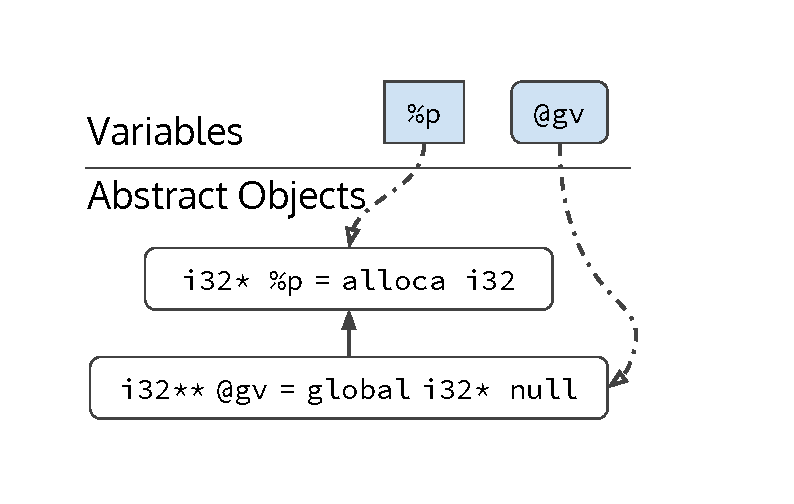
\includegraphics[trim={14mm 10mm 0 0},clip,width=1.5\linewidth]{figures/structsens/Partial-SSA.pdf}
    \subcaption{Points-to graph}
    \label{structsens/fig/partialssa:pt}
  \end{minipage}
  \caption{Partial SSA Example}
  \label{structsens/fig/partialssa}
\end{figure}


\section{Structure-Sensitive Approach}
\label{structsens/sect/approach}

Our analysis approach adds more detail to object abstractions, which
serve both as sources and as targets of points-to edges, allowing a
more detailed representation of the heap. Although our approach is
applicable to C/C++ analysis in general, it is best to see it in
conjunction with the LLVM bitcode intermediate language. Just as LLVM
bitcode is a strongly-typed intermediate language, we assign types and
offsets to every abstract object value and its points-to
relationships. The challenge is that, unlike in the LLVM bitcode type
system, such information is not readily available by local inspection
of the code---it needs to be propagated by the analysis reasoning
itself.

We next discuss the various abstractions of our analysis, in
representing its input and output relations. Then, we express the main
aspects of our analysis as a set of inference rules.

\subsection{Abstractions}
\label{structsens/sect/abstractions}

Figure~\ref{structsens/fig/domains} presents the input and output
domains of our analysis. We represent functions as a subset of global
entities. Thus, $G$ contains all symbols referencing global
entities---everything starting with symbol ``\code{@}'' in LLVM
bitcode. Set $V$ holds temporaries only (i.e., virtual registers), and
not global variables. We represent the union of these two sets with
$P$, which stands for \emph{pointer variables} (i.e., any entity whose
value may hold some memory address). Our analysis only introduces the
set of abstract objects $O$, that correspond to memory locations.

\begin{figure}[ht]
  \centering
  \begin{tabular}{l@{\quad}l}
    \toprule
    $T$ & set of program types \\
    $L$ & set of instruction labels \\
    $C$ & program (integer) constants \\
    $V$ & set of virtual registers \\
    $G$ & set of global variables \\
    $F \subseteq G$ & program functions \\
    $P = V \cup G$ & pointer variables \\
    \midrule
    $O$ & set of abstract objects \\
    \bottomrule
  \end{tabular}
  \caption{Analysis Domains}
  \label{structsens/fig/domains}
\end{figure}

The LLVM IR defines an extensive instruction set. However, only a
small subset is relevant for the purposes of pointer
analysis. Figure~\ref{structsens/fig/llvm} presents a simplified
version of these relevant instructions. The first two instructions are
used to allocate memory on the stack and on the heap, respectively. As
previously discussed, \instr{alloca} instructions are used for
address-taken variables. They accept an extra type argument (absent in
\instr{malloc} instructions), which specifies the exact type of the
allocation (virtual registers are strongly typed), and the allocation
size is a constant. Next, we have \instr{cast} instructions, used
solely to satisfy LLVM's type checker since they do not change any
memory contents, and \instr{phi} instructions that choose a value
depending on the instruction's predecessor. Apart from the standard
\instr{load}/\instr{store} instructions, we have two more instructions
that, given a memory address operand, return a new address by adding a
relative offset that corresponds to either a field or an array
element. (Only \instr{load} instructions dereference memory, however.)
Finally,
%% Not clear to me why store can take a constant address but load cannot.
%% If constants can be handled via intermediate registers in one case,
%% they also can in the other.
we have call and return instructions. Call instructions may also
accept a variable (function pointer), as their first argument.

\begin{figure}[t]
  \centering
  \begin{tabular}{l@{\quad}l@{\qquad}l}
    \toprule
    \emph{LLVM Instruction}
    & \emph{Operand Types}
    & \emph{Description} \\
    \midrule
    $\allocainstr{p}{T}{nbytes}$
    & $V \!\times\! T \!\times\! C$
    & Stack Allocations
    \\
    $\mallocinstr{p}{nbytes}$
    & $V \!\times\! (V \cup C)$
    & Heap Allocations
    \\
    $\castinstr{p}{T}{q}$
    & $V \!\times\! T \!\times\! (P \cup C)$
    & (No-op) Casts
    \\
    $\phiinstr{p}{l_1 : a_1}{l_2 : a_2}$
    & $V \!\times\! (L \mapsto (P \cup C))^2$
    & SSA Phi Node
    \\
    $\loadinstr{p}{q}$
    & $V \!\times\! P$
    & Load from Address
    \\
    $\storeinstr{p}{q}$
    & $P \!\times\! (P \cup C)$
    & Store to Address
    \\
    $\fieldaccess{p}{q}{f}$
    & $V \!\times\! P \!\times\! C$
    & Address-of-field
    \\
    $\arrayaccess{p}{q}{idx}$
    & $V \!\times\! P \!\times\! (V \cup C)$
    & Address-of-array-index
    \\
    $\callinstr{p}{a_0}[a_1][a_2,\ldots,a_n]$
    & $V \!\times\! (F \cup V) \!\times\! (P \cup C)^n$
    & Function Call
    \\
    $\returninstr{p}$
    & $P \cup C$
    & Function Return
    \\
    \bottomrule
  \end{tabular}
  \caption[LLVM IR Instruction Set]{%
    LLVM IR Instruction Set. We also prepend a label $l \in L$ to each
    instruction (that we omit in this figure). Each such label can be
    used to uniquely identify its instruction. %
  }
  \label{structsens/fig/llvm}
\end{figure}


\paragraph{Abstract Objects.}
Our analysis defines several different kinds of abstract objects that
express the exact nature of the allocation. Any abstract object must
fall into one of the following categories:

\begin{minipage}{\linewidth}
  \renewcommand{\arraystretch}{1.5}
  \begin{tabular}{@{--\ }l@{\quad}p{0.87\textwidth}}
    $\alloc{o_i}$
    & A stack or heap allocation for instruction (allocation site) $i \in L$.
    \\[3pt]
    $\alloc{o_{i,\tp{T}}}$
    & A (heap) allocation for instruction $i \in L$, specialized for type
      $\tp{T} \in T$.
    \\[3pt]
    % $\alloc{o_{v,i}}$
    % & A stack allocation for instruction (allocation site) $i \in L$,
    % assigned to virtual register $v \in V$.
    % \\[3pt]
    $\alloc{o_{g}}$
    & A global allocation for global variable or function $g \in G$.
    \\[3pt]
    % $\alloc{o_{f}}$
    % & A global allocation for function $f \in F$.
    % \\[3pt]
    $\alloc{o.fld}$
    & A field subobject that corresponds to field ``$fld\,$'' of base object
      $\alloc{o} \in O$.
    \\[3pt]
    $\alloc{o[c]}$
    & An array subobject that corresponds to the element at constant
      index $c \in C$ of base object $\alloc{o} \in O$.
    \\[1pt]
    $\alloc{o[*]}$
    & An array subobject that corresponds to any elements at unknown
      indices of base object $\alloc{o} \in O$.
    \\
  \end{tabular}
\end{minipage}

\noindent
When not using any special notation, we shall refer to a generic
abstract object that could be of any of the above forms. This also
applies to the base object of the last three categories (which, thus,
serve as recursive definitions), allowing us to define arbitrarily
complex subobjects such as \(\alloc{o.f[4].g[*]}\).

By representing field and array subobjects as separate abstract
objects themselves, the handling of instructions that return addresses
anywhere but at the beginning of some allocation becomes
straightforward. As we shall see at
Section~\ref{structsens/sect/rules}, all our analysis has to do is
return the relevant abstract object that represents the given
subobject of its base allocation. This abstract subobject will have
its own distinct points-to set, which will be tracked separately from
that of its base allocation or any of the rest of its fields. Thus, it
will allow the analysis to retain a certain degree of precision that
would be otherwise impossible.
% for a field-insensitive approach.

\vspace{0.5em}
\noindent
Our analysis computes four main
relations:
\begin{description}
\item[Variable points-to edges.] Edge $\vpt{p}{o} \in P \times O$
  records that pointer variable (either virtual register or global
  variable) $\var{p}$ may point to abstract object $\alloc{o}$. Note
  that virtual registers that correspond to source variables will
  always point to a single object: the corresponding stack
  allocation. Temporaries introduced by LLVM bitcode, though, may
  point to many abstract objects.
\item[Dereference edges.] Edge $\derefpt{po}{o} \in O \times O$
  records that abstract object $\alloc{po}$ may point to abstract
  object $\alloc{o}$. Any object that has a non-empty points-to set
  (i.e., the object has outgoing dereference edges) may represent a
  pointer. Dereference edges can only be established by \instr{store}
  instructions.
\item[Abstract object types.] The partial function
  $\typefunc: O \nrightarrow T$ records the type of an abstract
  object. An abstract object can be associated with one type at most,
  or none at all. Since our analysis uses types to filter redundant
  derivations, the more types it establishes for abstract objects, the
  more points-to edges it will compute.
  %
  Figure~\ref{structsens/fig/typeinf} establishes some basic type
  relations between the subobjects created by the analysis.
\item[Call-graph edges.] Edge $i \xrightarrow{calls} f \in L \times F$
  records that invocation site $i$ may call function $f$. This also
  accounts for indirect calls that use function pointers.
\end{description}

\begin{figure}[t]
  \begin{math}
    \inferrule* [left=Struct Type\;]
    {\alloctype{o} = \tp{S}
      \\ \gtype{\tp{S}.f} = \tp{F}}
    {\alloctype{o.f} = \tp{F}}
  \end{math}
  \;
  \begin{math}
    \inferrule* [left=Array Type\;]
    {\alloctype{o} = [\tp{T}]
      \\ c \in C}
    {\alloctype{o[*]} = \tp{T}
      \\ \alloctype{o[c]} = \tp{T}}
  \end{math}
  \caption{Basic Type Inferences for Abstract Objects.}
  \label{structsens/fig/typeinf}
\end{figure}


\subsection{Techniques - Rules}
\label{structsens/sect/rules}

Figure~\ref{structsens/fig/rules} presents the main aspects of the
analysis as a set of inference rules. The first two rules handle stack
and heap allocation instructions. All they do is create a new abstract
object representing the given allocation site, and assign it to the
target variable. In the case of stack allocation, we also record the
type of the object, since it is available at the allocation site. The
next pair of rules handle global allocations for global variables and
functions, respectively, in a similar way. In contrast to the previous
rules, we create abstract objects for all global entities, regardless
of any instructions (since their allocation in LLVM bitcode is
implicit), and record their types.

\begin{figure}[h!t]
  \begin{math}
    \inferrule* [left=Stack\;]
    {\allocainstr[i]{p}{T}{nbytes}}
    {\vpt{p}{o_{i}}
      \\ \alloctype{o_{i}} = \tp{T}}
  \end{math}
  \qquad
  \begin{math}
    \inferrule* [left=Heap\;]
    {\mallocinstr[i]{p}{nbytes}}
    {\vpt{p}{o_{i}}}
  \end{math}
  \\

  \begin{math}
    \inferrule* [left=Global\;]
    {\constant{f} \in F}
    {\cpt{f}{o_f}
      \\ \alloctype{o_f} = \gtype{f}}
    \qquad
    \inferrule*
    {\var{g} \in (G \setminus F)
      \\ \vartype{g} = \tp{T\,*}}
    {\vpt{g}{o_g}
      \\ \alloctype{o_g} = \tp{T}}
  \end{math}
  \\
  % \begin{math}
  %   \inferrule* [left=Field\;]
  %   {\alloctype{o} = \tp{S}
  %   \\ \exists \, \code{\tp{S}.fld}}
  %   {\exists \, \alloc{o.fld}
  %   \\ \alloctype{o.fld} = \codetype{\tp{S}.fld}}
  % \end{math}
  % \\

  % \begin{math}
  %   \inferrule* [left=Array\;]
  %   {\alloctype{o} = \tp{[T$\times$N]}}
  %   {\exists \, \alloc{o[*]}
  %   \\ \alloctype{o[*]} = \tp{T}}
  %   \quad
  %   \inferrule*
  %   {\alloctype{o} = \tp{[T$\times$N]}
  %   \\ \arrayaccess[i]{p}{q}{c}
  %   \\ \vartype{q} = \alloctype{o}}
  %   {\exists \, \alloc{o[c]}
  %   \\ \alloctype{o[c]} = \tp{T}}
  % \end{math}
  % \\
  \begin{math}
    \inferrule* [left=Cast\;]
    {\castinstr[i]{p}{T}{q}
      \\ \vpt{q}{o}}
    {\vpt{p}{o}}
  \end{math}
  \qquad
  \begin{math}
    \inferrule* [left=Phi\;]
    {\phiinstr[i]{p}{l_1 : a_1}{l_2 : a_2}}
    {\forall j:\ \opt{a_j}{o} \;\Rightarrow\; \opt{p}{o}}
  \end{math}
  \\

  \begin{math}
    \inferrule* [left=Load\;]
    {\loadinstr[i]{p}{q}
      \\ \vpt{q}{po}
      \\ \derefpt{po}{o}}
    {\vpt{p}{o}}
  \end{math}
  \quad
  \begin{math}
    \inferrule* [left=Store\;]
    {\storeinstr[i]{p}{q}
      \\ \vpt{p}{po}
      \\ \vpt{q}{o}}
    {\derefpt{po}{o}}
  \end{math}
  \\

  \begin{math}
    \inferrule* [left=Field\;]
    {\fieldaccess[i]{p}{q}{f}
      \\ \vpt{q}{o}
      \\ \alloctype{o} = \tp{S}
      % TODO consider adding \\ f \in \fields{S}
      \\ \vartype{q} = \tp{S\,*}}
    {\vpt{p}{o.f}}
  \end{math}
  \\

  \begin{math}
    \inferrule* [left=Array -- Const\;]
    {\arrayaccess[i]{p}{q}{c}
      \\ \vpt{q}{o}
      \\ \alloctype{o} = [\tp{T}]
      \\ \vartype{q} = [\tp{T}]\,\code{*}}
    {\vpt{p}{o[c]}}
  \end{math}
  \\

  \begin{math}
    \inferrule* [left=Array -- Var\quad \;]
    {\arrayaccess[i]{p}{q}{\var{j}}
      \\ \vpt{q}{o}
      \\ \alloctype{o} = [\tp{T}]
      \\ \vartype{q} = [\tp{T}]\,\code{*}}
    {\vpt{p}{o[*]}}
  \end{math}
  \\
  
  \begin{math}
    \inferrule* [left=Call\;]
    {\callinstr[i]{p}{a_0}[a_1][a_2,\ldots,a_n]
      \\ \opt{a_0}{o_f}
      \\ f \in F }
    {i \xrightarrow{calls} f(\op{p_1},\, \op{p_2},\, \ldots,\,
      \op{p_n})
      \\ \forall j:\ \opt{a_j}{o} \;\Rightarrow\; \opt{p_j}{o}}
  \end{math}
  \\

  \begin{math}
    \inferrule* [left=Ret\;]
    {\callinstr[i]{p}{a_0}
      \\ i \xrightarrow{calls} f(\ldots)
      \\ \returninstr[j]{q}
      \\ j \in \body{f}
      \\ \vpt{q}{o}}
    {\vpt{p}{o}}
  \end{math}
  \\

  \begin{math}
    \inferrule* [left=Heap-bp\;]
    {\mallocinstr[i]{p}{nbytes}
      \\ \castinstr[j]{w}{T\,*}{q}
      \\ \vpt{q}{o_{i}}}
    {\vpt{p}{o_{i,\tp{T}}}
      \\ \alloctype{o_{i,\tp{T}}} = \tp{T}}
  \end{math}
  \caption{Inference Rules}
  \label{structsens/fig/rules}
\end{figure}


For cast instructions, we copy any object that flows in the points-to
set of the source variable to the points-to set of the target
variable. Phi instructions are treated similarly, but we have to
consider both of the instruction's operands, regardless of their
corresponding labels, since our result must be an
over-approximation.

% Stores
Store instructions are the only way in which the analysis establishes
dereference edges. For a store instruction, $\storeinstr{p}{q}$, we have
to perform the following:% steps:

\begin{enumerate}
\item First, find the corresponding abstract objects that the two
  instruction operands point to, by following their outgoing variable
  points-to edges. Namely:
  \begin{inparaenum}[(i)]
  \item the memory allocation of the value to be stored (abstract
    object $\alloc{o}$), and
  \item the memory allocation that $\alloc{o}$ is going to be stored
    into (abstract object $\alloc{po}$).
  \end{inparaenum}
\item Then, establish a dereference edge between any two such abstract
  objects returned, expressing that object $\alloc{po}$ may point to
  object $\alloc{o}$.
\end{enumerate}
The first step simply bypasses the indirection introduced by LLVM
bitcode, where operands are represented as virtual registers that
point to memory locations.
% Loads
Load instructions perform the opposite operation, and thus are treated
symmetrically. For instruction $\loadinstr{p}{q}$, we first
\begin{inparaenum}[(i)]
\item find the corresponding abstract object that the address operand
  may point to (abstract object $\alloc{po}$),
\item then follow any outgoing dereference edge of object $\alloc{po}$
  to get any memory location $\alloc{po}$ may point to (object
  $\alloc{o}$), and finally
\item establish a new variable points-to edge for target variable
  $\var{p}$, recording that $\var{p}$ may now also point to object
  $\alloc{o}$.
\end{inparaenum}

The next three rules (\textsc{Field, Array--Const, Array--Var}) model field sensitivity. The rule
handling field accesses, such as $\fieldaccess{p}{q}{f}$, finds any
object $\alloc{o}$ that base variable $\var{q}$ may point to, and
returns $\alloc{o}\,$'s relevant field subobject
$\alloc{o.f}$. However, a key element is that $\alloc{o}$
is only considered as a base object if its type matches the declared
(struct) type of $\var{q}$ (recall that LLVM bitcode is strongly
typed). This precludes any untyped heap allocations as possible base
objects. Otherwise, the analysis would end up creating untyped field
subobjects too, further fueling imprecision. Thus, we are able to
maintain an important invariant of our structure-sensitive analysis:
\emph{only create field (or array) subobjects whose types we are able
  to determine}. Effectively, LLVM bitcode  imposes
\emph{strong typing on variables}, while our analysis extends the treatment
to \emph{abstract objects}.

Array element accesses are treated similarly and they, too, maintain
this invariant. However, we distinguish array accesses using a
constant index from those using a variable (i.e., unknown)
index. In the former case, we return the array subobject
$\alloc{o[c]}$, which represents the subobject at index
$c$. In the latter case, we return $\alloc{o[*]}$, which represents
the \emph{unknown} index. Essentially, this treatment allows our
analysis to track independently the points-to sets of array indices that are
statically known to be different, yielding a form of
\emph{array-sensitivity}.

Call and return instructions as modeled as assignments:
\begin{inparaenum}[(i)]
\item from any actual argument $a_j$ to its respective formal
  parameter $f_j$, and
\item from any returned value $\var{q}$ to the target variable of the
  call instruction $\var{p}$.
\end{inparaenum}
Like cast instructions, they simply copy the points-to sets from the
assignment's source to its target. However, the rule that handles call
instructions also records call-graph edges. When the function operand
$a_0$ may point to abstract object $o_f$, representing function $f$,
we record an edge from the given call site to function $f$. This
handles both direct and indirect calls (i.e., via function pointers).
% REVIEW: not entirely accurate; implementation uses filters on this
% case
% Note that no type checking needs to be performed by the analysis at
% this point. The type correctness of the call is ensured by the LLVM
% bitcode type system.

\paragraph{How to produce type information for unknown objects.}
%Allocation-site+Type Abstraction.}
Our analysis only allows taking the address of fields of objects 
whose type is known. This prevents loading and storing from/to fields
of objects without types. Such objects can only be used as identity
markers. Yet C and C++ allow the creation of untyped objects. Their handling
is a key element of the analysis.

The \textsc{Heap-bp} rule implements the \emph{use-based
back-propagation} technique~\cite{ecoop/LiTSX14,aplas/LivshitsWL05,aplas/SmaragdakisBKB15}, which creates multiple abstract
objects per (untyped) allocation site. The rule states that when an (untyped)
heap object $\alloc{o_i}$ (allocated at instruction $i$)
flows to some cast instruction $j$, where it is cast to type \tp{T}, we
augment the points-to set of $i$'s target variable $\var{p}$ with a
new abstract object $\alloc{o_{i,\tp{T}}}$, specialized for the given
type. The insight behind this rule is that, even when the program
performs an allocation via a type-agnostic routine like
\code{malloc()}, the allocation will be later cast to its intended
type before being used. By using this technique, the original untyped
allocation will be prevented from creating any untyped subobjects, but
as soon as the possible type of the allocation is discovered, the new
abstract typed object will succeed where the untyped one has failed.
Note that instructions $i$ and $j$ 
%are in no way related. They
could occur in distant parts of the program, as long as the analysis
can establish that the object allocated at instruction $i$ flows to
$j$.

This treatment successfully deals with generic
allocation wrappers or factory methods. In this case, the wrapped
allocation will flow to multiple cast instructions, and thus create
multiple typed variations of the original object. However, in each
case, only the object with the correct matching type will be used as a
base for any subsequent address-of-field instructions.
The rest of the objects will be filtered, since they are
indeed irrelevant.


\subsection{Partial Order of Abstract Objects}

As the observant reader may have noticed, the rules of
Figure~\ref{structsens/fig/rules} about accesses or array elements are
not sound. Consider the example of
Figure~\ref{structsens/fig/array}. Variable $\var{p}$ points to a heap
allocation. Three different store instructions take place:
\begin{inparaenum}[(i)]
\item one that stores $\code{\&i}$ to index 1,
\item one that stores $\code{\&j}$ to index 3, and
\item one that stores $\code{\&k}$ to some variable index.
\end{inparaenum}
When loading from index 1, the analysis has to return both
$\code{\&i}$ and $\code{\&k}$ (since the value of variable $\var{idx}$
may be equal to 1), but not $\code{\&j}$, which is stored to a
different index. Conversely, when loading from a variable index, the
analysis has to return all three addresses, since the index could be
equal to any constant.

\begin{figure}[ht]
\begin{cppcode}
int i, j, k, idx;
...
int **p = malloc(...);
p[1] = &i;
p[3] = &j;
p[idx] = &k;
int *x = p[1];  // yields $\{ i, k \}$
int *y = p[2];  // yields $\{ k \}$
int *z = p[j];  // yields $\{ i, j, k \}$
\end{cppcode}
  \caption{Accessing array elements.}
  \label{structsens/fig/array}
\end{figure}

Using our array-sensitive approach, we ensure that indices 1, 3, and
``$*$'' (unknown) are associated with separate points-to sets that are
not merged. To handle loads correctly, though, we have to be able to
reason about implicit associations of abstract objects, due to
possible index aliases. Thus, we say that object
$\alloc{o[*]}$ ``generalizes'' object $\alloc{o[c]}$ (for the same
base object $\alloc{o}$), since loading from $\alloc{o[*]}$ must
always return a superset of the objects returned by loading from
$\alloc{o[c]}$, for any constant $c$. This concept extends even to
deeply nested subobjects. For instance, an object 
$\alloc{o.f_1[*][2].f_2[*]}$ generalizes object
$\alloc{o.f_1[4][2].f_2[*]}$.

We can think of this binary relation between abstract objects as a
partial order over domain $O$ and define it appropriately.

\begin{defn}{\emph{Abstract Object Generalization Order.}}
  An abstract object $\alloc{y} \in O$ \emph{generalizes} an abstract
  object $\alloc{x}$, denoted $\alloc{x} \sqsubseteq \alloc{y}$, if
  and only if:

\begin{gather*}
  \alloc{x} = \alloc{y}
  \\
  \lor
  \\
  (\, \alloc{x} = \alloc{p[*]}\ \lor\ \alloc{x} = \alloc{p[c]} \,)\
  \land\ \alloc{y} = \alloc{q[*]}\
  \land\ \alloc{p} \sqsubseteq \alloc{q}
  \\
  \lor
  \\
  (\alloc{x} = \alloc{p.f}\
  \land\ \alloc{y} = \alloc{q.f}\
  \land\ \alloc{p} \sqsubseteq \alloc{q})
  \\
  \lor
  \\
  (\alloc{x} = \alloc{p[c]}\
  \land\ \alloc{y} = \alloc{q[c]}\
  \land\ \alloc{p} \sqsubseteq \alloc{q})
\end{gather*}
\end{defn}

\noindent
Intuitively, $\alloc{o_1} \sqsubseteq \alloc{o_2}$ holds when
$\alloc{o_1}$ can be turned to $\alloc{o_2}$ by substituting any of
its constant array indices with
``$*$''. Figure~\ref{structsens/fig/poset} gives an example of such
ordering. The direction of the edges is from the less to the more
general object.

\begin{figure}[ht]
  \centering
  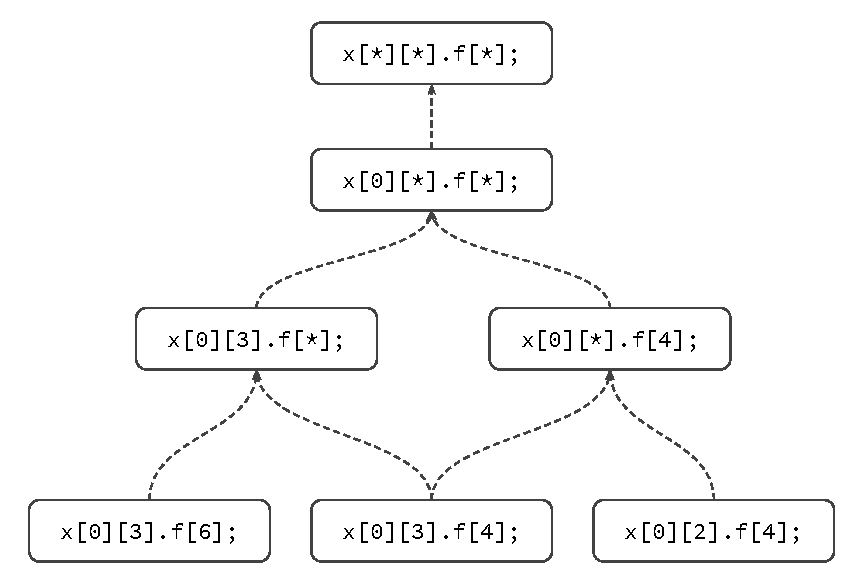
\includegraphics[clip,width=0.80\linewidth]{figures/structsens/Partial-Order.pdf}
  \caption[Abstract Object Ordering]{%
    Abstract Object Ordering -- Example: Nodes are abstract
    objects. An edge $(\, \alloc{s},\alloc{t} \,)$ denotes that object
    $\alloc{s}\:$ is generalized by object $\alloc{t}\:$ (i.e.,
    $\, \alloc{s} \sqsubseteq \alloc{t}\, $).}
  \label{structsens/fig/poset}
\end{figure}

Given this partial order, it suffices to add the two rules of
Figure~\ref{structsens/fig/rules:star} to account for possible index
aliases. The first rule states that the points-to set of a (less
general) object, such as $\alloc{o[c]}$, is a superset of the
points-to set of any object that generalizes it, such as
$\alloc{o[*]}$. The second rule modifies the treatment of load
instructions, so that they may return anything in the points-to set of
not just the object we load from (such as $\alloc{o}[*]$), but also of
objects that it generalizes (such as $\alloc{o[c]}$). In this way, the
general and specific points-to sets are kept distinct, while their
subset relationship is maintained.

\begin{figure}[ht]
  % \begin{math}
  %   \inferrule*
  %   {\alloc{o} \in O}
  %   {\alloc{o} \le \alloc{o}}
  % \end{math}
  % \quad
  % \begin{math}
  %   \inferrule*
  %   {\alloc{o_1} \le \alloc{o_2}
  %     \\ \alloc{o_1[c]}, \alloc{o_2[*]} \in O}
  %   {\alloc{o_1[c]} \le \alloc{o_2[*]}}
  % \end{math}
  % \\
  % \begin{math}
  %   \inferrule*
  %   {\alloc{o_1} \le \alloc{o_2}
  %     \\ \alloc{o_1.f}, \alloc{o_2.f} \in O}
  %   {\alloc{o_1.f} \le \alloc{o_2.f}}
  % \end{math}
  % ~
  % \begin{math}
  %   \inferrule*
  %   {\alloc{o_1} \le \alloc{o_2}
  %     \\ \alloc{o_1[c]}, \alloc{o_2[c]} \in O}
  %   {\alloc{o_1[c]} \le \alloc{o_2[c]}}
  % \end{math}
  % ~
  % \begin{math}
  %   \inferrule*
  %   {\alloc{o_1} \le \alloc{o_2}
  %     \\ \alloc{o_1[*]}, \alloc{o_2[*]} \in O}
  %   {\alloc{o_1[*]} \le \alloc{o_2[*]}}
  % \end{math}
  % \\
  \begin{math}
    \inferrule* [left=Match\;]
    {\alloc{o_1} \sqsubseteq \alloc{o_2}
      \\ \derefpt{o_2}{o}}
    {\derefpt{o_1}{o}}
  \end{math}
  \quad
  \begin{math}
    \inferrule* [left=Load II\;]
    {\loadinstr[i]{p}{q}
      \\ \vpt{q}{o_2}
      \\ \alloc{o_1} \sqsubseteq \alloc{o_2}
      \\ \derefpt{o_1}{o}}
    {\vpt{p}{o}}
  \end{math}
  \\
  \caption{Associating array subobjects via their partial order.}
  \label{structsens/fig/rules:star}
\end{figure}


\subsection{Soundness}

As stated by Avots et al. \cite{icse/AvotsDLL05}: ``\textit{A C
  pointer alias analysis cannot be strictly sound, or else it would
  conclude that most locations in memory may point to any memory
  location.}''
%
As in the PCP points-to analysis \cite{icse/AvotsDLL05}, our approach
tries to maintain precision at all times, even if this means that the
analysis is not sound in some cases.
%
Instead of trying to be as conservative as possible, we choose to opt
for precision and increase soundness by selectively supporting
well-established code patterns or idioms (such as using
\code{malloc()} to allocate many objects of different types).
%

The soundness assumptions of our analysis are that:
\begin{inparaenum}[(i)]
\item objects are allocated in separate memory spaces
  \cite{icse/AvotsDLL05}, and 
\item every (concrete) object has a single type throughout its
  lifetime.
\end{inparaenum}
%
Hence, our analysis would be unsound when a union type is used to
modify the same concrete object using two different types, since this
violates the second assumption. However, our analysis would be a good fit for
programs that use \emph{discriminated unions} (e.g., unions that
depend on a separate \emph{tag} field to determine the exact type of
the object), since it would create a different abstract object for
every type of the union, so that each such abstract object would
represent the subset of concrete objects with the same tag value.

In general, the single-type-per-lifetime assumption is reasonable for
most objects, but would be prohibitive in some cases---especially so
when the code relies on low-level assumptions about the byte layout of
the objects. For instance, our base approach would not be able to
meaningfully analyze code that uses a custom memory
allocator. Instead, the analysis would need to be extended so that it
models calls to the allocator by creating new abstract objects.

Finally, the analysis must be able to discover all associated types
for any given object, to retain its soundness. For simplicity, we
have only considered cast instructions as places where the
analysis discovers new types, but it is easy to supply additional type
hints by considering more candidates. For instance, an
exception object of unknown type may be allocated and then thrown, by
calling the \code{cxa::throw()} function in the C++ exception handling
ABI, without any intervening cast. However, we can use the
accompanying \emph{typeinfo} object (always supplied as the second
argument to \code{cxa::throw()}) to recover its true type and hence
create a typed abstract exception object. To the best of our
knowledge, such special treatment is needed only in rare cases, and
the analysis can be easily extended to handle them.


\section{Analyzing C++}
\label{structsens/sect/cxx}

LLVM bitcode is a representation well-suited for C. However, for OO
languages such as C++, high-level features are
translated to low-level constructs.  A classic example is dynamic
dispatch, through virtual methods. Virtual-tables are represented as
constant arrays of function pointers, and virtual calls are, in turn,
translated to a series of indirect access instructions.

\begin{figure}[ht]
  \begin{minipage}[b]{.5\linewidth}
%define void @func() {
% %b=alloca %class.B, // B b;
% ...
%
%}

\begin{bitcode}
%class.B = type { i32 (...)**, ...}

;; translation of bp->foo(), for
;; B *bp;
%1 = bitcast %bp to i32 (%class.B*)***
%2 = load i32 (%class.B*)** %1
%3 = getelementptr i32 (%class.B*)** %2, 1
%4 = load i32 (%class.B*)* %3
call i32 %4 (%class.B* %bp)
\end{bitcode}
    \subcaption{C++ virtual call compiled to LLVM bitcode}
    \label{structsens/fig/vcall:bitcode}
  \end{minipage}
  \begin{minipage}[b]{.5\linewidth}
    \centering
    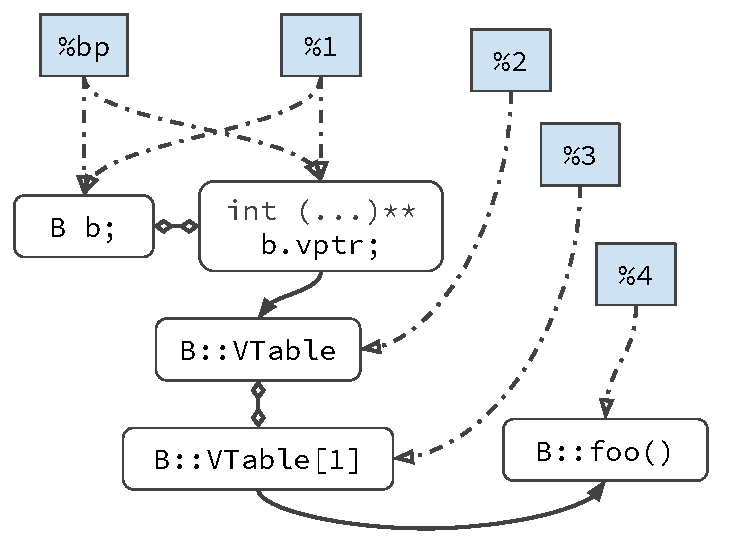
\includegraphics[trim={0 0 0 0},clip,width=1\linewidth]{figures/structsens/Virtual-Call.pdf}
    \subcaption{Points-to graph}
    \label{structsens/fig/vcall:ptgraph}
  \end{minipage}
  \caption{C++ Virtual Call Example}
  \label{structsens/fig/vcall}
\end{figure}

Figure~\ref{structsens/fig/vcall:bitcode} presents (a simplified
version of) the LLVM bitcode for such a translation. A virtual call
has to
\begin{inparaenum}[(i)]
\item load the v-pointer of the class instance (at offset 0),
\item index into the returned v-table (at the corresponding offset of
  the function being called),
\item then load the returned function pointer to get the exact address
  of the function, and
\item finally call the function.
\end{inparaenum}
By employing the techniques we have described so far, our
structure-sensitive analysis is well-equipped to deal with such an
involved pattern, and precisely resolve the function to be called.

Figure~\ref{structsens/fig/vcall:ptgraph} shows what our analysis
computes (assuming $\var{\%bp}$ points to variable $\var{b}$). Only a
minor addition is required: anything that points to an object should
also point to its first field (at byte offset 0). Hence, both
$\var{\%bp}$ and $\var{\%1}$ (after the cast) will point both to
(stack-allocated) object $\alloc{b}$, and to its v-pointer field
subobject $\alloc{b.vptr}$. The first load instruction will return the
v-table. Indexing into the v-table will return the corresponding array
element subobject, which will maintain its own independent (singleton)
points-to set, due to array-sensitivity. Finally, the second load
instruction will return the exact function that the v-table points to,
at the given offset.


\section{Enhancements}
\label{structsens/sect/addons}

Section~\ref{structsens/sect/approach} presented only the essential
parts of a structure-sensitive points-to analysis, but there can be
many enhancements worth discussing at this point. In this section, we
will list a few of the most valuable ones for a practical
implementation.

\subsection{Pointer Arithmetic}

In C/C++, given a pointer ``\mintinline{c++}{P *ptr}'', expressions
such as
\begin{inparaenum}[(i)]
\item ``\mintinline{c++}{(*ptr).fld}'',
\item ``\mintinline{c++}{ptr->fld}'', and
\item ``\mintinline{c++}{ptr[0].fld}''
\end{inparaenum}
are equivalent (and will be translated to the same LLVM bitcode
instruction). Hence, a pointer analysis must be able to reason about
such code patterns and map them to the same abstract (sub)object. In
LLVM IR, all such field accesses would be canonicalized to the third
form. In fact, all pointers in LLVM bitcode are treated as pointers to
arrays of objects (even when they point to a single
one).\footnote{This is exactly the reason for the first (frequently
  zero) index of the often misunderstood \code{getelementptr} LLVM
  bitcode instruction (see
  \url{http://llvm.org/docs/GetElementPtr.html}).}  Regarding the
possible choices of analysis inputs (discussed in
Chapter~\ref{chapter:intro}), such translations are certainly a point
in favor of choosing an intermediate representation such as LLVM
bitcode, so that the analysis need not concern itself with superfluous
syntactic constructs.

However, we have not so far delved into the various pointer arithmetic
idioms that are supported by C/C++ and that we would like for our
structure-sensitive analysis to support as well. A pointer in C is a
memory address, which is a numeric value. One can perform arithmetic
operations on a pointer just as with other numeric values. For
instance, the expression ``\mintinline{c++}{ptr+3}'' is equivalent to
``\mintinline{c++}{&ptr[3]}'' (which corresponds to the aforementioned
3rd form, as per LLVM's canonicalization).  Again LLVM's translation
can be very helpful in narrowing the complexity of the input
language. To see how our analysis can be extended to support pointer
arithmetic, we first have to briefly present LLVM's GEP instruction,
since this is what all types of element accesses (and pointer
arithmetic operations) are normally translated to.

\paragraph{The GEP Instruction.} The actual LLVM bitcode instruction
that is responsible for all types of element accesses is
\instr{getelementptr} (GEP). The GEP instruction accepts a base
pointer argument and one or more index arguments. It can be used to
retrieve any inner element of an arbitrarily nested structure. Its
general form is:

\[
  \mintinline{llvm}{
    %ptr = getelementptr %base, %idx1, %idx2, %idx3,
  }
  \ldots
\]

Assuming that \code{\%base} may point to an array of objects (in the
general case), the first index selects an element of this
array. (Expressions such as ``\mintinline{c++}{ptr->fld}''---being
equivalent to ``\mintinline{c++}{ptr[0].fld}''---implicitly refer to
the first element and thus produce a zero first index.)
%
Any index after the first corresponds to a field or array element
access.
% A variable can only be used in place of \code{\%idx1} (to
% index into the base pointer) or in any subsequent array indices (as
% opposed to field indices that always require a constant index).
Even
though the generic form of GEP may contain multiple indices to be able
to return the address of deeply nested elements, in practice, such
complex GEP instructions are split into multiple chained GEPs with at
most 2 indices.
%
Each one will descend in a single field or array index, roughly
corresponding to the \emph{address-of-field} and
\emph{address-of-array-index} instructions that we have previously
shown. Returning the address corresponding to a complex access path
such as ``\mintinline{c++}{ptr->f[4].g[k]}'' will require as many GEPs
as the depth of the access path: two field and two array accesses,
four in total.
%
Note that GEP instructions do not perform any memory dereference (as
the \instr{load} instruction does), but only compute a relative
offset.

So far we have not examined GEP instructions whose first index is
non-zero (thus retrieving the address of an element other than the
first, given a base pointer array). Fortunately, we can further
decompose such instructions to a GEP instruction with a single
non-zero index and a second GEP instruction of 2 indices, whose first
index is always zero.

\begin{figure}[h!t]
  \centering
  \begin{minipage}[b]{.4\linewidth}
    \centering
    \begin{bitcode}
      %ptr = getelementptr %b, 7, %v1, 8
    \end{bitcode}
    \subcaption{Complex GEP instruction}\label{structsens/fig/gep1}
  \end{minipage}%
  \qquad
  \begin{minipage}[b]{.4\linewidth}
    \centering
    \begin{bitcode}
      %t1 = getelementptr %b, 7
      %t2 = getelementptr %t1, 0, %v1
      %ptr = getelementptr %t2, 0, 8
    \end{bitcode}
    \subcaption{Decomposed GEP instruction}
    \label{structsens/fig/gep2}\par\vfill
  \end{minipage}
  \caption{Decomposition of GEP instructions}
  \label{structsens/fig/gep}
\end{figure}

Figure~\ref{structsens/fig/gep} demonstrates such a decomposition that
breaks a complex GEP instruction into multiple simpler ones. The last
two instructions of the decomposed version of
Figure~\ref{structsens/fig/gep2} correspond to our familiar notions of
\emph{address-of-array-index} and \emph{address-of-field}
instructions. Thus, we can dispense with GEP's overloaded behavior and
keep our inference rules almost intact. However, we have to augment
the analysis to support a single-index GEP, just like the first
instruction of Figure~\ref{structsens/fig/gep2}. Essentially, such
instructions perform a pointer increment operation and are of special
interest, since they alone should suffice for most translations of
dynamically allocated arrays and pointer arithmetic operations that
we are interested in.

\begin{figure}[h!t]
  \begin{math}
    \inferrule* [left=Stack\;]
    {\allocainstr[i]{p}{T}{nbytes}}
    {\vpt{p}{o_{i}[0]}
      \\ \alloctype{o_{i}[0]} = \tp{T}}
  \end{math}
  \qquad
  \begin{math}
    \inferrule* [left=Heap\;]
    {\mallocinstr[i]{p}{nbytes}}
    {\vpt{p}{o_{i}[0]}}
  \end{math}
  \\

  \begin{math}
    \inferrule* [left=Pointer -- Var I\quad \;]
    {\ptraccess[i]{p}{q}{\var{j}}
      \\ \gtype{q} = \tp{T\,*}
      \\ \vpt{q}{o[k]}
      \\ \alloctype{o[k]} = \tp{T}}
    {\vpt{p}{o[*]}}
  \end{math}
  \\

  \begin{math}
    \inferrule* [left=Pointer -- Var II\quad \;]
    {\ptraccess[i]{p}{q}{\var{j}}
      \\ \gtype{q} = \tp{T\,*}
      \\ \vpt{q}{o[*]}
      \\ \alloctype{o[*]} = \tp{T}}
    {\vpt{p}{o[*]}}
  \end{math}
  \\

  \begin{math}
    \inferrule* [left=Pointer -- Const I\;]
    {\ptraccess[i]{p}{q}{c}
      \\ \gtype{q} = \tp{T\,*}
      \\ \vpt{q}{o[*]}
      \\ \alloctype{o[*]} = \tp{T}}
    {\vpt{p}{o[*]}}
  \end{math}
  \\

  \begin{math}
    \inferrule* [left=Pointer -- Const II\;]
    {\ptraccess[i]{p}{q}{c}
      \\ \gtype{q} = \tp{T\,*}
      \\ \vpt{q}{o[k]}
      \\ \alloctype{o[k]} = \tp{T}
      \\\\  k + c \in \indices{T}}
    {\vpt{p}{o[k+c]}}
  \end{math}
  \\

  \begin{math}
    \inferrule* [left=Pointer -- Const III\;]
    {\ptraccess[i]{p}{q}{c}
      \\ \gtype{q} = \tp{T\,*}
      \\ \vpt{q}{o[k]}
      \\ \alloctype{o[k]} = \tp{T}
      \\\\  k + c \notin \indices{T}}
    {\vpt{p}{o[*]}}
  \end{math}
  \caption{Dealing with pointer arithmetic}
  \label{structsens/fig/ptrarithm}
\end{figure}

Figure~\ref{structsens/fig/ptrarithm} presents an extension of our
analysis to handle such pointer increment operations. The first two
rules replace the previous ones (for base allocations) by slightly
changing the objects we allocate to resemble the first
elements of potential array allocations. In cases where an instruction
allocates a single object, such zero offsets may be redundant but
facilitate the increment operations of the following rules. The next
two rules handle pointer increment operations that use a variable
index \(\var{j}\). In both cases, the result should disregard any
prior index of the object pointed by \var{q}, and replace it with the
``\(*\)'' index. The last three rules handle pointer increment
operations that add a constant \(c\). The first of them states that
adding a constant index to an already unknown index makes no
difference and simply propagates the same special object
(\(\alloc{o[*]}\)). In the last two rules, \(\var{q}\) points to an
object with a constant index instead (\(\alloc{o[k]}\)), whereupon the
analysis tries to compute a new constant index \(k+c\) and point to
the relevant object (\(\alloc{o[k+c]}\)). However, such general
treatment could potentially lead to the creation of infinite
objects. To avoid this, we only point to \(\alloc{o[k+c]}\) if the new
index \(k+c\) statically appears in the source code (and is associated
with type \(\tp{T}\)). Otherwise, the analysis falls back to using
\(\alloc{o[*]}\).

To identify what static indices are associated with each type we
define the function \emph{indices} as follows:
\begin{equation*}
  \begin{split}
    \indices{T} =
    \{ 0 \}
    & \cup
    \{ c :  \exists \; \ptraccess{p}{q}{c} \,\land\, \gtype{q} = \tp{T\,*}
    \}
    \\
    & \cup \{ c :  \exists \; \arrayaccess{p}{q}{c} \,\land\, \gtype{q} = [\tp{T}]
    \}
  \end{split}
\end{equation*}


\subsection{Abstract Object Aliases}

There are cases where two abstract objects, such as \(\alloc{o}\) and
\(\alloc{o[0]}\) may coincide (i.e., map to the same memory
address). This applies to both zero indices of arrays and the first
fields of structs. Ignoring such object aliases could lead to unsound
results, e.g., when dereferencing an object without taking the
points-to sets of its aliases into account.

To handle such cases, the analysis should treat aliased abstract
objects as an equivalence class.

\begin{defn}{\emph{Abstract Object Aliases.}}
  We define the \emph{alias} equivalence relation \(\sim\) on the set
  of abstract objects \(O\) as the transitive, symmetric, and
  reflexive closure of the binary relation \(\simless\), so that given
  two abstract objects \(\alloc{x},\, \alloc{y} \in O\),
  \(\alloc{x}\, \simless\; \alloc{y}\), if and only if:
  \begin{gather*}
    \alloc{y} = \alloc{x[0]}
    \\
    \lor
    \\
    \alloc{y} = \alloc{x.f} \land \offsetof(f) = 0
  \end{gather*}
  where \(\offsetof(f)\) returns the byte offset of a struct field
  \(f\).
\end{defn}

\begin{figure}[ht]
  \begin{math}
    \inferrule* [left=Deref$^+$\;]
    {\alloc{o_1} \sim \alloc{o_2}
      \\ \derefpt{o}{o_1}}
    {\derefpt{o}{o_2}}
  \end{math}
  \;
  \begin{math}
    \inferrule* [left=InvDeref$^+$\;]
    {\alloc{o_1} \sim \alloc{o_2}
      \\ \derefpt{o_1}{o}}
    {\derefpt{o_2}{o}}
  \end{math}
  \;
  \begin{math}
    \inferrule* [left=Vpt$^+$\;]
    {\alloc{o_1} \sim \alloc{o_2}
      \\ \vpt{v}{o_1}}
    {\vpt{v}{o_2}}
  \end{math}
  \caption{Extending the analysis with aliased objects.}
  \label{structsens/fig/aliases}
\end{figure}

Figure~\ref{structsens/fig/aliases} extends the dereference and
variable points-to edges computed by the analysis due to object
aliases. The first rule states that whenever an object points to
another, it should also point to any aliases of the latter. The second
rule inverses this notion: when an object is pointed by another, it
should also be pointed by its aliases. The third rule is analogous to
the first one, but extends variable points-to edges instead.


\subsection{Type Compatibility}

We have used type equality as a filter for redundant derivations in
the inference rules we have presented so far. In practice, however,
this could prove too restrictive and lead to the exclusion of
perfectly valid derivations. For instance, consider the trailing
padding that C compilers append to struct types for proper
alignment. The structure type of Figure~\ref{structsens/fig/unpadded}
would be transformed to that of Figure~\ref{structsens/fig/padded}, as
most compilers would append a padding field of 7 bytes so that the
total size becomes 16---a multiple of the largest alignment of any of
its members (in this case, a multiple of 8 due to field \code{p}).

\begin{figure}[h!t]
  \centering
  \begin{minipage}[b]{.4\linewidth}
    % \captionsetup{singlelinecheck=false,justification=justified}
    \centering\large
    \begin{cppcode}
      struct s1 {
        char *p;     /* 8 bytes */
        char c;      /* 1 byte */
      };
    \end{cppcode}
    \subcaption{Unpadded Structure Type}\label{structsens/fig/unpadded}
  \end{minipage}%
  \qquad
  \begin{minipage}[b]{.4\linewidth}
    % \captionsetup{singlelinecheck=false,justification=justified}
    \centering\large
    \begin{cppcode}
      struct s1 {
        char *p;     /* 8 bytes */
        char c;      /* 1 byte */
        char pad[7];
      };
    \end{cppcode}
    \subcaption{Padded Structure Type}
    \label{structsens/fig/padded}
  \end{minipage}
  \caption{Structure Alignment and Padding}
  \label{structsens/fig/padding}
\end{figure}

However, had a padded struct (or class) type been inherited by
another, then the compiler could in some cases use the unpadded
version as the base type, since the padding could be redundant if new
fields were considered.\footnote{In LLVM IR, the name of the unpadded
  version of the type would contain a \code{.base} suffix to
  distinguish it from the original padded version.} If strict type
equality was required by the analysis, then this could prohibit
objects of a derived type to be used as the receiver arguments of
inherited methods at places where the analysis employed its type
filters (such as in \emph{address-of-field} instructions).

\begin{figure}[h!t]
  \begin{minipage}[b]{.3\linewidth}
    \begin{lcppcode}
      struct s1 {
        char *p;
        char c;

        void meth() {
          char *c1 = this->p;
          ...
        }
      };

      struct s2 : s1 {
        char b;
      };
    \end{lcppcode}
    \subcaption{C++ Source}\label{structsens/fig/typeincompat:cxx}
  \end{minipage}%
  \qquad
  \begin{minipage}[b]{.6\linewidth}
    \centering\large
    \begin{bitcodelinum}
      ; Types

      %struct.s1 = type { i8*, i8, [7 x i8] }
      %struct.s1.base = type { i8*, i8 }
      %struct.s2 = type { %struct.s1.base, i8, [6 x i8] }

      ; Methods

      define void @s1_meth(%struct.s1* %this) {
        ; the second 0 offset is that of field p
        %1 = getelementptr %struct.s1* %this, i64 0, i32 0
        ...
      }
    \end{bitcodelinum}
    \subcaption{LLVM Bitcode}
    \label{structsens/fig/typeincompat:bitcode}
  \end{minipage}
  \caption{Padding, Inheritance, and Type Incompatibility}
  \label{structsens/fig/typeincompat}
\end{figure}

Figure~\ref{structsens/fig/typeincompat} illustrates this case. The
generated LLVM bitcode uses the unpadded version of \code{s1} as its
first field (inherited objects are always translated to normal fields,
in bitcode), to reduce its overall padding to just 6 bytes. Had an
object \(\alloc{o}\) of type \(\tp{s2}\) flowed to the points-to set
of \code{s1::meth()}'s \code{this} argument, it would be filtered out
in the \code{getelementptr} instruction due to type inequality of
\(\tp{s1}\) and \(\tp{s2}\), per our \textsc{Field} inference rule
of Section~\ref{structsens/sect/approach}.

Note that, had the \code{\%struct.s1.base} type not existed for padding
reasons, our object alias rules of Figure~\ref{structsens/fig/aliases}
alone would suffice in this case:
\begin{compactitem}[\(\cdot\)]
\item the \(\alloc{o.f_{s1}}\) subobject, representing the first field
  of \(\alloc{o}\) (i.e., its \(\tp{s1}\) base object), would be
  considered an alias of \(\alloc{o}\), since its byte offset is zero
\item \code{\%this} would, hence, also point to \(\alloc{o.f_{s1}}\)
  besides \(\alloc{o}\)
\item \code{getelementptr} would not filter out \(\alloc{o.f_{s1}}\),
  since its type would be equal to the expected declared type
  \(\tp{s1}\)
\item \code{\%1} would finally point to the \(\alloc{o.f_{s1}.p}\)
  subobject.
\end{compactitem}

Such reasoning can be encoded in the following complex derivation:

\vspace{0.5em}
\begin{minipage}{\linewidth}
  \small
  \begin{math}
    \inferrule* [left=Field\;]
    {\inferrule* [left=Vpt$^+$\;]
      {\alloc{o.f_{s1}} \sim \alloc{o}
        \\ \vpt{this}{o}}
      {\vpt{this}{o.f_{s1}}}
      \\ \fieldaccess[11]{\%1}{this}{p}
      \\ \alloctype{o.f_{s1}} = \gtype{\var{this}} = \tp{s1}
    }
    {\vpt{\%1}{o.f_{s1}.p}
      \\ \alloctype{o.f_{s1}.p} = \tp{char\,*}}
  \end{math}
\end{minipage}
\vspace{0.5em}

We can relax our type equality constraints by introducing a notion of
\emph{type compatibility}. We list the following cases of compatible
types:
\begin{itemize}[--]
\item a type is type compatible with itself (making the relation
  reflexive)
\item an array type \tp{T[]} is type compatible with another array
  type \tp{U[]}, if
  \begin{inparaenum}[(i)]
  \item its component type \tp{T} is type compatible with \tp{U}, and
  \item they are either of the same size (e.g., \tp{T[5]}, \tp{U[5]}),
    or at least one of them does not specify a size (e.g., \tp{T[7]},
    \tp{U[]})
  \end{inparaenum}
\item a function type
  \(\tp{R} (\tp{T}_1, \tp{T}_2, \tp{T}_3, ..., \tp{T}_n)\) is type
  compatible with function type
  \(\tp{S} (\tp{U}_1, \tp{U}_2, \tp{U}_3, ..., \tp{T}_n)\)
  if
  \begin{inparaenum}[(i)]
  \item their return types \tp{R} and \tp{S} are type
    compatible, and
  \item so are their arguments types (i.e., \(\tp{T}_i\) is type
    compatible with \(\tp{U}_i\) for every \(i \in 1,\ldots ,n\))
  \end{inparaenum}
\item a function type
  \(\tp{R} (\tp{T}_1, \tp{T}_2, \tp{T}_3, \ldots, \tp{T}_n)\) is also
  type compatible with the variadic function type
  \(\tp{S} (\tp{U}_1, \tp{U}_2, \tp{U}_3, \ldots, \tp{U}_m, \ldots)\)
  if
  \begin{inparaenum}[(i)]
  \item \(m < n\),
  \item their return types \tp{R} and \tp{S} are type compatible, and
  \item so is the common subset of their arguments types (i.e.,
    \(\tp{T}_i\) is type compatible with \(\tp{U}_i\) for every
    \(i \in 1,\ldots ,m\))
  \end{inparaenum}
\item a struct type \(\tp{S}_1\) (consisting of fields
  \(\tp{F}_1, \tp{F}_2, \tp{F}_3, \ldots, \tp{F}_n\), in that order),
  is type compatible \emph{up to field} \(k\) with struct type
  \(\tp{S}_2\) (consisting of fields
  \(\tp{Q}_1, \tp{Q}_2, \tp{Q}_3, \ldots, \tp{Q}_m\)),
  %
  if field type \(\tp{F}_i\) is type compatible with
  \(\tp{Q}_i\) for every \(i \in 1,\ldots ,k\);
  %
  moreover, \(\tp{S}_1\) and \(\tp{S}_2\) are type compatible, if they
  are type compatible up to field \(m\) and \(m\) equals \(n\)
\item a struct type \(\tp{S}_1\) is an \emph{eligible base} of type
  \(\tp{S}_2\), if the first field of \(\tp{S}_2\), \(\tp{F}_1\), is
  type compatible with \(\tp{S}_1\) up to field \(n\)---where \(n\) is
  the number of fields of \(\tp{F}_1\)% \footnote{In the example of
    % Figure~\ref{structsens/fig/typeincompat}, \code{\%struct.s1} is an
    % eligible base of \code{\%struct.s2} because
    % \code{\%struct.s1.base} is type compatible with \code{\%struct.s1}
    % up to field 2.}
\item a pointer type \tp{T*} is type compatible with another pointer
  type \tp{U*}, if
  \begin{compactenum}[(1)]
  \item its component type \tp{T} is type compatible with \tp{U},
  \item either \tp{T} or \tp{U} is \code{char}, or
  \item \tp{U} is (transitively) an \emph{eligible base} of \tp{T}.
  \end{compactenum}
\end{itemize}

Our type compatibility rules are deliberately geared towards
structural compatibility (as is our overall structure-sensitive
approach). Restricting the type compatibility rules to comply with some
specific C/C++ standard would not work, since by the time the compiler
has transformed the code to LLVM bitcode, the various transformations
and optimizations up to this point would almost certainly violate such
rules.

Henceforth, we will use the notation ``\typecompat{\tp{T}}{\tp{U}}''
to signify that type \tp{T} is type compatible with \tp{U}, according
to the previous rules. Even though we will forgo rewriting any
previous inference rules of our analysis to make use of the type
compatibility relation, the reader should assume that any strict type
equality premise clauses therein, such as
``\(\alloctype{o} = \tp{T}\)\,'', should be replaced with the more
generic ``\(\typecompat{\alloctype{o}}{\tp{T}}\)''.

As a final note, every struct type can be viewed as an array of bytes
(as hinted by our type compatibility rules). A field could be accessed
in such a way, via its byte
offset. Figure~\ref{structsens/fig/byteoffset} identifies such
accesses and treats them accordingly.

\begin{figure}[ht]
  \begin{math}
    \inferrule* [left=Byte Offset\;]
    {\ptraccess[i]{p}{q}{c}
      \\ \gtype{q} = \tp{char\,*}
      \\ \vpt{q}{o}
      \\ \alloctype{o} = \tp{T}
      \\\\ \offsetof(\tp{T}.f) = c}
    {\vpt{p}{o.f}}
  \end{math}
  \caption{Accessing field via byte offset.}
  \label{structsens/fig/byteoffset}
\end{figure}


\subsection{Copying Memory Areas}

There are various functions in C that copy memory from a pointer to
another (e.g., \code{memcpy()}, \code{memmove()}, \code{bcopy()},
etc). Such operations have an obvious effect on the points-to sets of
objects: an object that is copied to another location should have its
points-to set copied as well.

\begin{figure}[ht]
  \begin{math}
    \inferrule* [left=Memcpy Base\;]
    {\callinstr[i]{p}{a_0}[a_1][a_2,\ldots]
      \\ i \xrightarrow{calls} \texttt{memcpy}\,(\ldots)
      \\ \opt{a_1}{o_{to}}
      \\ \opt{a_2}{o_{from}}
      \\\\ \alloctype{o_{from}} = \tp{T}
      \\ \alloctype{o_{to}} = \tp{U}
      \\ \typecompat{\tp{T}}{\tp{U}}
    }
    {\cp{o_{from}}{o_{to}}}
  \end{math}
  \\

  \begin{math}
    \inferrule* [left=Memcpy Rec I\;\;\:]
    {\cp{o_1}{o_2}
      \\ \alloctype{o_1[*]} = \tp{T}
      \\ \alloctype{o_2[*]} = \tp{U}
      \\ \typecompat{\tp{T}}{\tp{U}}}
    {\cp{o_1[*]}{o_2[*]}}
  \end{math}
  \\

  \begin{math}
    \inferrule* [left=Memcpy Rec II\;\:]
    {\cp{o_1}{o_2}
      \\ \alloctype{o_1[c]} = \tp{T}
      \\ \alloctype{o_2[c]} = \tp{U}
      \\ \typecompat{\tp{T}}{\tp{U}}}
    {\cp{o_1[c]}{o_2[c]}}
  \end{math}
  \\

  \begin{math}
    \inferrule* [left=Memcpy Rec III\;]
    {\cp{o_1}{o_2}
      \\ \alloctype{o_1.f} = \tp{T}
      \\ \alloctype{o_2.f} = \tp{U}
      \\ \typecompat{\tp{T}}{\tp{U}}}
    {\cp{o_1.f}{o_2.f}}
  \end{math}
  \\

  \begin{math}
    \inferrule* [left=Memcpy Deref$^+$\;]
    {\cp{o_{from}}{o_{to}}
      \\ \derefpt{o_{from}}{o}}
    {\derefpt{o_{to}}{o}}
  \end{math}
  \caption{Handling memory copying.}
  \label{structsens/fig/memcpy}
\end{figure}

To support memory copying, we first identify copied objects. The first
rule of Figure~\ref{structsens/fig/memcpy} marks that an abstract
object \(\alloc{o_{from}}\) was copied to another object
\(\alloc{o_{to}}\), if a (direct or indirect) call to the
\code{memcpy()} routine was made and these were the objects pointed by
\code{memcpy()}'s operands. (Note that we use the objects pointed by
the actual and not the formal arguments, to avoid associating objects
of unrelated \code{memcpy} calls. This could also be achieved with
context-sensitivity based on call-sites.) Additionally, we require
that the objects are of compatible types, to filter imprecision. The
next three rules of Figure~\ref{structsens/fig/memcpy} extend our
notion of copied objects recursively, by marking subobjects as well
(as long as they remain type compatible with each other). The last rule
performs the propagation of the points-to set of an object that was
copied to another.


\section{Evaluation}
\label{structsens/sect/eval}

We compare our structure-sensitive analysis to a re-implementation of
the Pearce et al. \cite{paste/PearceKH04,toplas/PearceKH07} analysis
in \cclyzer{}, that also operates over the full LLVM bitcode
language. We will refer to this analysis as \pearce{}. Both analyses
were implemented using Datalog, and include the enhancements of
Section~\ref{structsens/sect/addons} and a few more to deal with
various features (hidden copies of struct instances due to
pass-by-value semantics, constant expressions, etc.) that arise in
practice.

%
For our benchmark suite, we use the 8 largest programs (in terms of
bitcode size) in \emph{GNU Coreutils},\footnote{Our original selection
  included the 10 largest coreutils, but \code{dir} and \code{vdir}
  turned out to be identical to \code{ls} and are maintained mostly
  for backwards-compatibility reasons.}  and 14 executables from
\emph{PostgreSQL}. We use a 64-bit machine with two octa-core Intel
Xeon E5-2667 (v2) CPUs at 3.30GHz and 256GB of RAM. The analysis
is single-threaded and occupies a small portion of the RAM. We use
the LogicBlox Datalog engine (v.3.10.14) and LLVM v.3.7.0.

%% Figure~\ref{structsens/fig/stats:misc} presents some general
%% metrics on the input and output of each analysis:
%% \begin{inparaenum}[(i)]
%% \item number of call-graph edges (allocation site to function),
%% \item number of abstract objects created by the analysis, and
%% \item running time (excluding constant overhead that bootstrap both
%%   analyses).
%% \end{inparaenum}

%% \begin{figure}[tb!p]
%%   \setlength{\tabcolsep}{4pt}
%%   \centering
%%   \begin{tabular}{l@{\quad}r r@{\quad}rr r@{\quad}rr}
%%     \toprule
%%     &
%%     & \multicolumn{3}{c}{\emph{Structure-sensitive}}
%%     & \multicolumn{3}{c}{\pearce}
%%     \\
%%     \cmidrule(lr){3-5} \cmidrule(l){6-8}
%%     \multirow{2}{*}{Benchmark}
%%     & \multirow{2}{*}{Size}
%%     & call-graph & abstract & running & call-graph & abstract & running \\
%%     &
%%     & edges      & objects  & time    & edges      & objects  & time
%%     \\
%%     \midrule
%%     cp       & 720K & 3205 & 68166 & 29.25s & 3117 & 3380 & 13.62s \\
%%     df       & 456K & 1812 & 38919 & 20.68s & 1781 & 2236 & 11.09s \\
%%     % dir      & 604K & 2654 & 66469 & 22.67s & 2110 & 2783 & 12.57s \\
%%     du       & 608K & 2424 & 49592 & 29.77s & 2312 & 3008 & 21.96s \\
%%     ginstall & 692K & 3185 & 59893 & 25.12s & 3101 & 3207 & 14.32s \\
%%     ls       & 604K & 2654 & 66469 & 22.43s & 2110 & 2783 & 13.35s \\
%%     mkdir    & 384K & 1466 & 21900 & 17.35s & 1413 & 1641 & 11.43s \\
%%     mv       & 648K & 2932 & 55619 & 25.50s & 2848 & 3015 & 12.20s \\
%%     sort     & 608K & 2480 & 75360 & 34.25s & 2447 & 2955 & 21.40s \\
%%     % vdir     & 604K & 2654 & 66469 & 23.28s & 2110 & 2783 & 13.21s \\
%%     \midrule
%%     clusterdb  & 528K & 1390 & 167605 & 33.90s & 1353 &  4461 & 11.89s \\
%%     createdb   & 528K & 1412 & 168068 & 30.58s & 1375 &  4480 & 11.07s \\
%%     createlang & 572K & 1928 & 133869 & 25.67s & 1891 &  4275 & 12.68s \\
%%     createuser & 532K & 1435 & 171115 & 31.07s & 1398 &  4569 &  9.31s \\
%%     dropdb     & 524K & 1361 & 165966 & 31.26s & 1324 &  4399 & 12.72s \\
%%     droplang   & 572K & 1936 & 133912 & 24.38s & 1899 &  4278 & 12.55s \\
%%     dropuser   & 524K & 1356 & 165615 & 30.45s & 1319 &  4386 & 12.15s \\
%%     ecpg       & 1.2M & 5713 &  59252 & 38.47s & 5713 &  5219 & 29.11s \\
%%     pg-ctl     & 488K & 1615 & 118689 & 23.36s & 1578 &  3655 &  9.14s \\
%%     pg-dumpall & 572K & 2110 & 184276 & 32.18s & 2073 &  5153 & 11.95s \\
%%     % pg-dump    & 1.4M & & & & & & \\
%%     pg-isready & 464K & 1302 & 108622 & 21.54s & 1265 &  3343 & 11.25s \\
%%     pg-rewind  & 556K & 1943 & 136915 & 25.56s & 1906 &  4301 & 11.48s \\
%%     pg-upgrade & 604K & 2501 & 151967 & 26.49s & 2464 &  4965 & 11.80s \\
%%     psql       & 1.4M & 5925 & 460522 & 67.76s & 5552 & 14025 & 25.28s \\
%%     \bottomrule
%%   \end{tabular}
%%   \caption{Analysis Input and Output Metrics. The first column is
%%     benchmark bitcode size (in bytes). The second (resp. fifth) column is the
%%     number of call-graph edges. The third (resp. sixth) column is the
%%     number of abstract objects created. The fourth (resp. seventh) column
%%     is the running time of the analysis.}
%%   \label{structsens/fig/stats:misc}
%% \end{figure}

\begin{figure}[t]
  \setlength{\tabcolsep}{4pt}
  \centering
  \begin{tabular}{l@{\quad}r r@{\quad}rr rr}
    \toprule
    &
    &
    & \multicolumn{2}{c}{\emph{Structure-sensitive}}
    & \multicolumn{2}{c}{\pearce}
    \\
    \cmidrule(lr){4-5} \cmidrule(l){6-7}
    \multirow{2}{*}{Benchmark}
    & \multirow{2}{*}{Size}
    & call-graph & abstract & running & abstract & running \\
    &
    & edges      & objects  & time    & objects  & time
    \\
    \midrule
    cp       & 720K & 3205 & 68166 & 29.25s & 3380 & 13.62s \\
    df       & 456K & 1812 & 38919 & 20.68s & 2236 & 11.09s \\
    du       & 608K & 2424 & 49592 & 29.77s & 3008 & 21.96s \\
    ginstall & 692K & 3185 & 59893 & 25.12s & 3207 & 14.32s \\
    ls       & 604K & 2654 & 66469 & 22.43s & 2783 & 13.35s \\
    mkdir    & 384K & 1466 & 21900 & 17.35s & 1641 & 11.43s \\
    mv       & 648K & 2932 & 55619 & 25.50s & 3015 & 12.20s \\
    sort     & 608K & 2480 & 75360 & 34.25s & 2955 & 21.40s \\
    \midrule
    clusterdb  & 528K & 1390 & 167605 & 33.90s &  4461 & 11.89s \\
    createdb   & 528K & 1412 & 168068 & 30.58s &  4480 & 11.07s \\
    createlang & 572K & 1928 & 133869 & 25.67s &  4275 & 12.68s \\
    createuser & 532K & 1435 & 171115 & 31.07s &  4569 &  9.31s \\
    dropdb     & 524K & 1361 & 165966 & 31.26s &  4399 & 12.72s \\
    droplang   & 572K & 1936 & 133912 & 24.38s &  4278 & 12.55s \\
    dropuser   & 524K & 1356 & 165615 & 30.45s &  4386 & 12.15s \\
    ecpg       & 1.2M & 5713 &  59252 & 38.47s &  5219 & 29.11s \\
    pg-ctl     & 488K & 1615 & 118689 & 23.36s &  3655 &  9.14s \\
    pg-dumpall & 572K & 2110 & 184276 & 32.18s &  5153 & 11.95s \\
    pg-isready & 464K & 1302 & 108622 & 21.54s &  3343 & 11.25s \\
    pg-rewind  & 556K & 1943 & 136915 & 25.56s &  4301 & 11.48s \\
    pg-upgrade & 604K & 2501 & 151967 & 26.49s &  4965 & 11.80s \\
    psql       & 1.4M & 5925 & 460522 & 67.76s & 14025 & 25.28s \\
    \bottomrule
  \end{tabular}
  \caption[Input and Output Metrics]{%
    Input and Output Metrics. The first column is benchmark bitcode
    size (in bytes). The second column is the number of call-graph
    edges (as computed by our analysis). The third (resp. fifth)
    column is the number of abstract objects created. The fourth
    (resp. sixth) column is the analysis running time.}
  \label{structsens/fig/stats:misc}
\end{figure}

Figure~\ref{structsens/fig/stats:misc} presents some general metrics
on the input and output of each analysis:
\begin{inparaenum}[(i)]
\item number of call-graph edges (allocation site to function),
\item number of abstract objects created by the analysis, and
\item running time (excluding constant overhead that bootstrap both
  analyses).
\end{inparaenum}

\begin{figure}[t]
  \setlength{\tabcolsep}{3pt}
  \centering
  \begin{tabular}{l r@{\quad}rr r@{\quad}rr}
    \toprule
    & \multicolumn{3}{c}{\emph{Structure-sensitive}}
    & \multicolumn{3}{c}{\pearce}
    \\
    \cmidrule(lr){2-4} \cmidrule(l){5-7}
    Benchmark
    & (\%) $|pt(v)| \rightarrow 1$
    & $2$
    & $3$
    & (\%) $|pt(v)| \rightarrow 1$
    & $2$
    & $3$
    \\
    \midrule
    % cp       & 2945 & 12.655 & 3.328 & 1997 &  10.497 & 3.664 \\
    % df       & 1650 & 10.475 & 1.590 & 1205 &   9.409 & 3.825 \\
    % dir      & 1883 & 15.730 & 4.399 & 1524 &  17.346 & 4.160 \\
    % du       & 2448 & 22.436 & 3.424 & 1691 &  48.356 & 3.856 \\
    % ginstall & 2771 & 10.439 & 1.663 & 2072 &   9.106 & 4.425 \\
    % ls       & 1883 & 15.730 & 4.399 & 1524 &  17.346 & 4.160 \\
    % mkdir    & 1534 &  8.207 & 3.154 &  978 &  11.548 & 3.588 \\
    % mv       & 2578 & 10.356 & 1.520 & 1806 &   9.843 & 4.098 \\
    % sort     & 2125 & 31.851 & 6.440 & 1628 & 123.681 & 7.450 \\
    % vdir     & 1883 & 15.730 & 4.399 & 1524 &  17.346 & 4.160 \\
    cp       & 35.42 & 11.56 & 9.03 & 24.02 & 2.91 & 3.51 \\
    df       & 35.98 & 13.15 & 8.37 & 26.28 & 1.98 & 4.38 \\
%    dir      & 33.23 &  6.09 & 8.81 & 26.90 & 3.57 & 2.67 \\
    du       & 37.06 & 10.51 & 7.54 & 25.60 & 2.00 & 2.95 \\
    ginstall & 36.31 & 14.24 & 8.28 & 27.15 & 7.44 & 3.14 \\
    ls       & 33.23 &  6.09 & 8.81 & 26.90 & 3.57 & 2.67 \\
    mkdir    & 36.11 &  8.43 & 9.65 & 23.02 & 2.00 & 4.35 \\
    mv       & 35.09 & 13.71 & 8.97 & 24.58 & 6.78 & 3.04 \\
    sort     & 29.20 &  5.25 & 9.65 & 22.37 & 1.47 & 2.53 \\
%    vdir     & 33.23 &  6.09 & 8.81 & 26.90 & 3.57 & 2.67 \\
    \midrule
    average  & 34.49 &  9.51 & 8.79 & 25.37 & 3.53 & 3.19 \\
    \midrule
    clusterdb  & 40.86 & 8.42 &  7.93 & 24.46 & 2.79 &  3.85 \\
    createdb   & 40.82 & 9.11 &  7.95 & 24.54 & 2.83 &  4.31 \\
    createlang & 42.72 & 8.87 & 11.89 & 25.62 & 4.10 &  4.78 \\
    createuser & 40.33 & 8.85 &  8.75 & 24.07 & 3.18 &  4.44 \\
    dropdb     & 40.59 & 8.69 &  7.96 & 23.97 & 2.91 &  4.00 \\
    droplang   & 42.68 & 8.86 & 11.88 & 25.67 & 4.10 &  4.75 \\
    dropuser   & 40.36 & 8.72 &  8.01 & 23.86 & 2.86 &  4.02 \\
    ecpg       & 16.72 & 1.22 &  0.52 & 15.14 & 0.30 & 42.64 \\
    pg-ctl     & 41.31 & 8.46 &  8.50 & 25.31 & 3.31 &  4.05 \\
    pg-dumpall & 40.52 & 7.10 &  7.21 & 27.74 & 3.10 &  4.61 \\
    pg-isready & 39.89 & 8.12 &  7.87 & 23.59 & 2.92 &  4.03 \\
    pg-rewind  & 44.74 & 7.55 &  8.56 & 31.39 & 2.75 &  3.76 \\
    pg-upgrade & 41.12 & 8.35 &  9.34 & 27.73 & 2.95 &  3.70 \\
    psql       & 38.62 & 5.81 &  9.33 & 25.61 & 2.31 &  3.20 \\
    \midrule
    average    & 39.38 & 7.72 &  4.55 & 24.91 & 2.89 &  6.87 \\
    \bottomrule
  \end{tabular}
  \caption[Variable points-to sets]{%
    Variable points-to sets. Proportion of resolved variables (that
    point to one abstract object), as well as variables with two or
    three points-to targets.}
  \label{structsens/fig/stats:var}
\end{figure}

Figure~\ref{structsens/fig/stats:var} compares the two analyses in
terms of the degree of resolving variable points-to targets. The first
column of each analysis lists the percentage of fully resolved
variables (virtual registers): \emph{how many point to a single
  abstract object}. This is the main metric of interest for most
analysis clients. The next two columns list the percentage of
variables that point to two/three objects.

It is evident that our structure-sensitive analysis fares consistently
better in fully resolving variable targets. Our analysis resolves many
more variables than \pearce{} does, for any of the available
benchmarks, with an average increase of $36\%$ across all coreutil
benchmarks and $58\%$ in the PostgreSQL benchmarks.  This is
\emph{despite using a finer-grained object abstraction than
  \pearce{}}: The ``abstract objects'' column of
Figure~\ref{structsens/fig/stats:misc} shows that our analysis
abstraction has \emph{one to two orders of magnitude more} abstract
objects than \pearce{}. Yet it succeeds at resolving many more
variables to a single (and much finer-grained) abstract object. (The
only benchmark instance in which \pearce{} somewhat benefits from its
coarse abstract object granularity is ecpg: a full $42.64\%$ of
variables point to 3, much coarser than ours, abstract objects.) Note
also that the \pearce{} analysis appears much better than it actually
is for meaningful cases, due to large amounts of low-hanging
fruit---e.g., global or address-taken variables, which are the single
target of some virtual register, due to the SSA representation.


\section{Summary}

We began this chapter by introducing the needs for a revised abstract
memory model for points-to analysis when analyzing C/C++, which can
fully support field sensitivity and maintain maximal structural
information for its abstract objects. We accomplish this by increasing
object granularity to force the creation of typed objects and by fully
distinguishing subobjects as well. We give a brief overview of our
techniques in Section~\ref{structsens/sect/overview}, and present some
limited background about the peculiarities of C/C++ and LLVM IR in
Section~\ref{structsens/sect/background}, regarding the complications
they pose to the problem of pointer analysis. We describe our
structure-sensitive points-to analysis in depth in
Section~\ref{structsens/sect/approach}, and discuss how the techniques
it employs make it suitable for analyzing C++ programs in
Section~\ref{structsens/sect/cxx}. In
Section~\ref{structsens/sect/addons} we present various enhancements,
essential for a realistic implementation. Finally, we evaluate our
approach by comparing it to a standard field-sensitive analysis in
Section~\ref{structsens/sect/eval}.

% TODO put in conclusions
% We presented a structure-sensitive points-to analysis for C and
% C++. The analysis attempts to always distinguish abstract objects and
% assign them a unique type (even when none is known at the point of
% object creation) as well as to discriminate between subobjects of a
% single object (array or structure instance). We describe the analysis
% in precise terms and show that its approach succeeds in maintaining
% precision when analyzing realistic programs. In our experience, the
% techniques we described are essential for analyzing C/C++ programs at
% the same level of precision as programs in higher-level languages.

%% \hl{TODO}

%% See Hind's Pointer Analysis: Haven’t We Solved This Problem Yet? 4.9
%% Section.

%% List of field-insensitive analyses:
%% \cite{antgrasshopper}

%% \cite{popl/ZhengR08}            % CFL

%% Field-based:
%% \cite{andersen:thesis,pldi/HeintzeT01a}

%% Field-sensitive:
%% \cite{paste/PearceKH04,paste/NystromKH04}

%% Field-sensitive lacks any description:
%% \cite{popl/HardekopfL09,cgo/HardekopfL11}

%% Steensgaard-like:
%% \cite{pldi/LattnerLA07}

%% % Test citation
%% \cite{oopsla/BravenboerS09}


%%% Local Variables:
%%% mode: latex
%%% TeX-master: "../thesis"
%%% End:


\chapter{%
  More Sound Static Handling of Java Reflection}
\label{chapter:reflection}
\epigraph{Mr. Treehorn treats objects like women, man.}{\textit{The Dude}}

In Chapter~\ref{chapter:structsens}, we targeted the problem of lost
structural information in C/C++ programs by employing a pointer
analysis that recovers lost memory structure via a variety of
techniques. In this chapter and the next, we shift our focus to Java:
a higher-level, strongly-typed language with no capabilities for direct
memory access.
%
Still, essential structural information is often lost in Java programs
too, yet for different reasons. As stated in
Chapter~\ref{chapter:intro}, a source of analysis imprecision,
especially in determining the types of abstract objects constructed by
the analysis, lies in the use of Java's reflection mechanism: the
ability to inspect and dynamically retrieve classes, methods, attributes,
etc. at runtime.

By using the Reflection API, Java programs can encompass dynamic
behavior. However, statically reasoning about the behavior of software
that uses reflection can be especially cumbersome.
%
Unfortunately, reflection is ubiquitous in large Java programs.
% static reflection handling is hard because of the ubiquity of reflection in real
% programs and because of the size of Java programs and libraries.
%
Any handling of reflection will be approximate, and overestimating its
reach in a large codebase can be catastrophic for precision and
scalability. In this chapter, we present an approach for handling
reflection with improved empirical soundness (as measured against
prior approaches and dynamic information), again, in the context of a
points-to analysis. Our approach is based on the combination of
string-flow and points-to analysis from past literature augmented with
\begin{inparaenum}[(a)]
\item substring analysis and modeling of partial string flow through
  string builder classes;
\item new techniques for analyzing reflective entities based on
  information available at their use-sites (similar to those presented
  in Chapter~\ref{chapter:structsens}).
\end{inparaenum}
% The resulting analysis is general, without any need for hand-tuning. 
In experimental comparisons with prior approaches, we demonstrate a
combination of both improved soundness (recovering the majority of
missing call-graph edges) and increased performance.

% achieves near-complete coverage of the target program: our static
% heuristics seem to truly offer an over-approximation of dynamic
% behavior, without sacrificing scalability. Whereas past studies have
% shown hundreds of methods (as much as 40\% of the dynamically
% reachable methods) to be statically undiscovered, we achieve over 97\%
% completeness at virtually no extra cost.

\section{Intro: Static Analysis and Java Reflection}
\label{reflection/sec:intro}

Whole-program static analysis is the engine behind several modern
programming facilities for program development and
understanding. Compilers, bug detectors, security checkers, modern
development environments (with automated refactorings, slicing
facilities, and auto-complete functionality), and a myriad other tools
routinely employ static analysis machinery. Even the seemingly simple
effort of computing a program's call-graph (i.e., which program
function can call which other) requires sophisticated analysis in
order to achieve precision in a modern language.

Yet, static whole-program analysis suffers in the presence of common
dynamic features, especially reflection. When a Java program accesses
a class by supplying its name as a run-time string, via the
\javasignature{Class.forName} library call, the static analysis has
very few available courses of action: It needs to either
conservatively over-approximate (e.g., assume that \emph{any} class
can be accessed, possibly limiting the set later, after the returned
object is used), or to perform a string analysis that will allow it to
infer the contents of the \code{forName} string argument. Both options
can be detrimental to the scalability of the analysis: the
conservative over-approximation may never become constrained enough by
further instructions to be feasible in practice; precise string
analysis is impractical for programs of realistic size.  It is telling
that \emph{no practical Java program analysis framework in existence
  handles reflection soundly} \cite{soundiness15}, although other
language features are modeled soundly.\footnote{In our context,
  \emph{sound} = over-approximate, i.e., guaranteeing that all
  possible behaviors of reflection operations are modeled.}

%
Full soundness is not practically achievable, but it can still be
approximated for the well-behaved reflection patterns encountered in
regular, non-adversarial programs.  Therefore, it makes sense to treat
soundness as a continuous quantity: something to improve on, even
though we cannot perfectly reach.  To avoid confusion, we use the term
\emph{empirical soundness} for the quantification of how much of the
dynamic behavior the static analysis covers. Computable metrics of
empirical soundness can help quantify how close an analysis is to the
fully sound result. Based on such metrics, one can make comparisons
(e.g., ``more sound'') to describe soundness improvements.

%An analysis is termed ``soundy'', when it is ``sound modulo
%well-known sources of unsoundness'', such as
%reflection \cite{soundiness15}.

%Empirical soundness is the quantification of the gap between soundy and
%(the unattainable) fully sound. The techniques presented in this
%chapter serve as a step in that direction: beyond soundy, yet not fully
%sound.


%After all, the reason to perform static
%analysis is to capture more program behaviors than a dynamic
%execution---the converse is a paradox that puts the value of the
%static analysis in question. Even if guaranteed full soundness is
%impractical, it is desirable to capture most actual behavior for the
%well-behaved reflection patterns encountered in regular,
%non-adversarial programs.

The second challenge of handling reflection in a static analysis is
\emph{scalability}.  The online documentation of the IBM \textsc{Wala}
library~\cite{www:wala-reflection} concisely summarizes the current
state of the practice, for \emph{points-to analysis} in the Java
setting.

\begin{quote}
  \emph{Reflection usage and the size of modern libraries/frameworks
    make it very difficult to scale flow-insensitive points-to
    analysis to modern Java programs. For example, with default
    settings, \textsc{Wala}'s pointer analyses cannot handle any
    program linked against the Java 6 standard libraries, due to
    extensive reflection in the libraries.}
\end{quote}

\noindent The same caveats routinely appear in the research
literature. Multiple published points-to analysis papers analyze
well-known benchmarks with reflection
disabled~\cite{popl/SmaragdakisBL11,pldi/KastrinisS13,ecoop/AliL12,ecoop/AliL13}.


A representative quote~\cite{popl/SmaragdakisBL11} illustrates:
\begin{quote}
  \emph{Hsqldb and jython could not be analyzed with reflection
    analysis enabled [...]  ---hsqldb cannot even be analyzed
    context-insensitively and jython cannot even be analyzed with the
    1obj analysis. This is due to vast imprecision introduced when
    reflection methods are not filtered in any way by constant strings
    (for classes, fields, or methods) and the analysis infers a large
    number of reflection objects to flow to several variables.  [...]
    For these two applications, our analysis has reflection reasoning
    disabled.  Since hsqldb in the DaCapo benchmark code has its main
    functionality called via reflection, we had to configure its entry
    point manually.}
\end{quote}

%\noindent
In this chapter, we describe an approach to analyzing reflection in the
Java points-to analysis setting.
%Points-to analysis consists
%of computing which objects (abstracted as allocation sites) a program
%variable can reference. The analysis is the backbone of many realistic
%static analyses, as it offers a scalable way to model heap behavior.
%
%Notably, both of the
%above quotes regarding the difficulties of reflection handling are in
%the context of points-to analyses.
%
Our approach requires no manual configuration and achieves
significantly higher empirical soundness without sacrificing
scalability, for realistic benchmarks and libraries (DaCapo Bach and
Java 7).
%% than those that past work failed to analyze.
% As we shall see, our analysis implements (and
%enables to run with full reflection support) the same points-to
%algorithms that in the past could not scale to some benchmarks, all
%using the Java 6 standard libraries, which the \textsc{Wala} documentation
%warns about. 
%
%There are two new technical elements in our work:
%
%\begin{bullets}
%\item We augment prior algorithms for inter-related reflection and
%points-to analysis \cite{aplas/LivshitsWL05,livshits:thesis} with a
%\emph{substring} analysis, as well as a string flow analysis.  
%%
%%While
%%past approaches have required user specifications to determine the
%%possible target of reflective calls whose input was partially dynamic,
%%we attempt to over-approximate without sacrificing scalability. For
%%instance, consider the case of a program that contains a constant
%%string, \code{"Handler"}, which partially matches reflection-accessible
%%entities of the program code---e.g., a class name
%%``\code{somePackage.EventHandler}'', or a method name
%%``\code{callbackHandler}''. If our string flow analysis determines that
%%this string flows (through standard Java API string operators such as
%%\code{+}, which resolves to \code{append} and \code{toString}) to the site
%%of a \code{forName} call, it will conservatively assume that the
%%reflection object (aka ``class object'') for class
%%\code{somePackage.EventHandler} can be returned at that
%%point. Similarly, if the \code{"Handler"} string (however augmented by
%%concatenations) flows to the site of a reflective call (such as
%%\javasignature{Class.getMethod}) that attempts to retrieve a method from a class
%%object containing method \code{callbackHandler}, the analysis will
%%compute that the call may return the reflection object for this
%%method.
%%
%The insight behind this treatment is that reflection is often used to
%dynamically access entities with partially known names, and the
%dynamic part of the configuration is limited to package prefixes,
%method name suffixes, etc. Thus, much of the dynamic information
%(i.e., other substrings contributing to the eventual string
%representing a class or member name) can be supplanted by
%mere over-approximation.
%
%
%%The merging
%%of string constants is a very common optimization technique that
%%significantly improves performance (TODO: citation needed).
%
%\item We introduce new techniques for inferring the result of
%  reflection calls based on how this result is used later in the
%  program. Consider, for instance, a sequence of program statements,
%  possibly remote to each other, yet with values flowing from one to
%  the next:
%
%\begin{code}
%\begin{small}
%\begin{verbatim}
%Class c1 = Class.forName(className);
%...      // c2 aliases c1
%Object o1 = c2.newInstance(); 
%...      // o2 aliases o1
%e = (Event) o2; 
%\end{verbatim}
%\end{small}
%\end{code}
%
%%String className = ... ;
%%
%%Object o = c.newInstance();
%%String methodName = ... ;
%%Method m = c.getMethod(methodName, ...);
%%m.invoke(o, ...);
%
%%If we know that the object held by \code{o} is the result of a reflection
%%operation (e.g., the return value of a \javasignature{Field.get} or a
%%\javasignature{Method.invoke} call) then we immediately get information on the
%%reflection call that produced \code{o}, by assuming that the cast is
%%intended to succeed. 
%
%Assuming that the cast is intended to succeed, we get information
%regarding the result of the \code{newInstance} call, which, in turn,
%informs the result of the \code{forName} call. That is, by keeping track
%of the flow of objects from an original call that accepts strings and
%produces reflection objects (such as a \code{forName} or a \code{getField}
%call) we infer that this string could have been the
%name of a subtype of \code{Event}. This effectively propagates
%information back to the source of an unknown object.
%
%Similar reasoning has been employed in other work
%\cite{aplas/LivshitsWL05,ecoop/LiTSX14}. Yet our approach generalizes
%past techniques significantly: we support patterns such as the above
%inter-procedurally and in full generality, leverage information from
%strings and not just casts, and introduce ``invented'' objects that
%materialize at the point of a cast and subsequently aid the analysis
%modeling.
%
%
%%%%SPACE (probably not only)
%% Our approach has three
%%differences.  First, our analysis is completely inter-procedural: we
%%allow the last two statements of the above example to occur in distant
%%methods, and leverage the base points-to analysis to track object
%%flow.  In contrast, all past techniques required  the cast
%%operation not only to be in the same method as the \code{newInstance}
%%(or other similarly treated calls) but also to post-dominate
%%it. Second, we leverage use-based information from strings, and not
%%just from casts. For instance, a \javasignature{Class.getMethod} or
%%\javasignature{Class.getField} call with a constant string parameter gives
%%information that can narrow down what the receiver \code{Class} object
%%may be. Lastly, we introduce ``invented'' objects that fully
%%materialize at the point of a cast and participate in the analysis
%%afterwards. In our example, if a special marker object is found to
%%flow to variable \code{o2} from a reflection call, in addition to
%%propagating information back to the reflection call, a new
%%invented object of type \code{Event} will be considered to exist
%%at the point of the cast, to represent all objects possibly missed. By
%%carefully balancing the amount of information propagated back to the
%%reflection call vs. the new objects invented at cast points, we trade
%%off scalability for soundness. For instance, if a cast does not
%%significantly narrow down the possible \code{Class} objects returned by
%%a distant \code{forName} call, we do not propagate information backwards
%%to the \code{forName} call site, as this would be detrimental to
%%precision and scalability. (The site would appear to create a many
%%different \code{Class} objects, which will propagate down and pollute
%%all intermediate reflective calls.)  Instead, in this case we will
%%only propagate an invented object forward.
%%
%%\end{bullets}
%%
%% ideas
%%that were earlier only applied intra-procedurally; it infers objects
%%based on string constants; and it creates usable abstract
%%representations of objects it cannot identify (whereas past work only
%%treated such objects as placeholders).
%
%\item We carefully tune the context-sensitivity and object
%  discrimination policies of our analysis to maintain scalability, by
%  avoiding an explosion in the number of entities. For instance, we
%  remove context-sensitivity from reflective method invocations and
%  object creation, although context-sensitivity is restored for
%  methods called directly (i.e., virtual or static calls) inside
%  reflectively called methods. Similarly, we merge the points-to
%  handling of all string objects representing method or field names
%  (but not class names), while still remembering (over-approximately)
%  which reflection entities they may refer to. Additionally, we merge
%  string factory objects (instances of library classes
%  \code{StringBuilder} or \code{StringBuffer}) despite the need to track
%  substring flow through them. Essentially, if a substring whose name
%  may refer to a reflection entity $E$ flows to \emph{any} string
%  factory, and \emph{any} string factory feeds into a reflective call,
%  reflection entity $E$ is inferred to possibly be the result of the
%  call. Intuitively, the above broad over-approximation does not affect
%  much the precision of our approach because the enabling conditions
%  provide a good filter and because precision is often restored in
%  practice when the code casts the result of a reflective call to a
%  certain type.
%
%We apply our approach to the \textsc{Doop} framework~\cite{oopsla/BravenboerS09} and
%evaluate it using the DaCapo benchmarks. We find that our techniques
%achieve very high empirical soundness, as measured in call-graph edges
%relative to
%%(several) 
%dynamic executions. For comparison, the earlier reflection treatment
%of \textsc{Doop}, which implemented the algorithm of Livshits et
%al.~\cite{aplas/LivshitsWL05},
%% without any of our enhancements, 
%missed many tens to hundreds of call-graph edges for each benchmark
%\cite{ecoop/AliL12,ecoop/AliL13} and even required
%manual configuration to achieve this result. Furthermore, we make no
%sacrifices in scalability: our analyses scale just as well as (or
%better than) the original \textsc{Doop} analyses even for modern large JDKs.
%
%As a result of carefully balancing the soundness and scalability of
%all techniques, our approach is more sound than past work, without
%sacrificing scalability. 
%
In experimental comparisons with the recent \textsc{Elf}
system~\cite{ecoop/LiTSX14} (itself improving over the reflection
analysis of the \textsc{Doop} framework~\cite{oopsla/BravenboerS09}),
our algorithm discovers most of the call-graph edges missing (relative
to a dynamic analysis) from \textsc{Elf}'s reflection analysis.  This
improvement in empirical soundness is accompanied by \emph{increased}
performance relative to \textsc{Elf}, demonstrating that near-sound
handling of reflection is often practically possible. Concretely, our
work in this chapter:
\begin{itemize}[\(\cdot\)]
%\item offers the first static handling of Java reflection that 
% exhibits both high empirical soundness and performance for
% sophisticated analyses and large-scale benchmarks, with no
% extra inputs;
\item introduces key techniques in static reflection handling that
  contribute greatly to empirical soundness. The techniques generalize
  past work from an intra-procedural to an inter-procedural setting
  and combine it with a string analysis;
\item shows how scalability can be addressed with appropriate tuning
  of the above generalized techniques;
\item thoroughly quantifies the empirical soundness of a static
  points-to analysis, compared to past approaches and to a dynamic
  analysis;
\item is implemented and evaluated on top of an existing open
  framework (\textsc{Doop}~\cite{oopsla/BravenboerS09}).
  % This can offer a platform for experimentation with sophisticated
  % static reflection handling, possibly also leading to good static
  % handling of other dynamic features (e.g., complex dynamic
  % loading).
\end{itemize}

%%%SPACE
%The rest of the chapter introduces important background on static
%reflection analysis (Section~\ref{reflection/sec:model}), presents our new
%techniques (Section~\ref{reflection/soundiness}), evaluates them
%(Section~\ref{reflection/sec:experiments}), and compares to related work
%(Section~\ref{reflection/sec:related}).


\section{Points-to Analysis in Java}
\label{reflection/sec:javapt}

In Chapter~\ref{chapter:structsens}, we presented a points-to analysis
for C/C++ that includes various enhancements to make it
structure-sensitive. Before presenting our enhancements towards better
handling of Java's reflection, we first present a typical points-to
analysis for Java and discuss its fundamental differences from
analyzing C/C++.

The domains of the analysis include:
\begin{compactitem}[\(\cdot\)]
\item variables, \(V\)
\item (class) types, \(T\)
\item fields, \(F\)
\item methods, \(M\)
\item abstract (heap) objects, \(H\)
\item instruction labels, \(L\)
\item and strings.
\end{compactitem}

\begin{figure}[t]
  \centering
  \begin{tabular}{l@{\quad}l@{\qquad}l}
    \toprule
    \emph{Java Instruction}
    & \emph{Operand Types}
    & \emph{Description} \\
    \midrule
    \(\newinstr{p}{C}\)
    & \(V \!\times\! T\)
    & Heap Allocations
    \\
    \(\castinstr{p}{T}{q}\)
    & \(V \!\times\! T \!\times\! V\)
    & Casts
    \\
    \(\moveinstr{p}{q}\)
    & \(V \!\times\! V\)
    & Assignments
    \\
    \(\fldloadinstr{p}{q}{f}\)
    & \(V \!\times\! V \!\times\! F\)
    & Field Loads
    \\
    \(\fldstoreinstr{p}{f}{q}\)
    & \(V \!\times\! F \!\times\! V\)
    & Field Stores
    \\
    \(\vcallinstr{p}{v}{meth}\)
    & \(V \!\times\! V \!\times\! M \!\times\! V^n\)
    & Virtual Calls
    \\
    \(\scallinstr{p}{C}{meth}\)
    & \(V \!\times\! T \!\times\! M \!\times\! V^n\)
    & Static Calls
    \\
    \(\returninstr{p}\)
    & \(V\)
    & Method Returns
    \\
    \bottomrule
  \end{tabular}
  \caption[Java Instruction Set]{%
    Java Instruction Set. We also prepend a label $l \in L$ to each
    instruction (that we omit in this figure). Each such label can be
    used to uniquely identify its instruction. %
  }
  \label{structsens/fig/javair}
\end{figure}

Figure~\ref{structsens/fig/javair} lists the basic Java instructions,
relevant to a points-to analysis. We note some key differences from
the C/C++ setting:
\begin{itemize}[--]
\setlength\itemsep{0.3em}
\item there are no pointer types, or any way to directly operate on
  memory addresses
\item there is a clear distinction between variables (allocated on the
  stack) and objects (allocated on the heap)
\item loads and stores need a field operand
\item there are two types of method call instructions:
  \begin{inparaenum}[(i)]
  \item virtual calls (that perform dynamic dispatch based on the
    dynamic type of the receiver), and
  \item static calls.
  \end{inparaenum}
\end{itemize}

\begin{figure}[h!t]
  \begin{math}
    \inferrule* [left=Alloc\,]
    {\newinstr[i]{p}{T}}
    {\vpt{p}{o_{i}}
      \\ \alloctype{o_{i}} = \tp{T}}
  \end{math}
  \\

  \begin{math}
    \inferrule* [left=Cast\,]
    {\castinstr[i]{p}{T}{q}
      \\ \vpt{q}{o_{i}}
      \\ \alloctype{o_{i}} = \tp{T'}
      \\ \subtypeof{T'}{T}}
    {\vpt{p}{o_{i}}}
  \end{math}
  \\

  \begin{math}
    \inferrule* [left=Move\,]
    {\moveinstr[i]{p}{q}
      \\ \vpt{q}{o_{i}}}
    {\vpt{p}{o_{i}}}
  \end{math}
  \\

  \begin{math}
    \inferrule* [left=Load\;]
    {\fldloadinstr[i]{p}{q}{f}
      \\ \vpt{q}{o_b}
      \\ \fieldpt{o_b}{f}{o}}
    {\vpt{p}{o}}
  \end{math}
  \\

  \begin{math}
    \inferrule* [left=Store\;]
    {\fldstoreinstr[i]{p}{f}{q}
      \\ \vpt{p}{o_b}
      \\ \vpt{q}{o}}
    {\fieldpt{o_b}{f}{o}}
  \end{math}
  \\

  \begin{math}
    \inferrule* [left=VCall\;]
    {\vcallinstr[i]{p}{v}{meth}
      \\ \vpt{v}{o}
      \\ \alloctype{o} = \tp{T}
      \\ \lookup{T}{meth} = \code{meth}\rq}
    {i \xrightarrow{calls} \code{meth}\rq\,(\ldots)
      \\ \vpt{this\(_{\,\code{meth}\rq}\)}{o}}
  \end{math}
  \\

  \begin{math}
    \inferrule* [left=SCall\;]
    {\scallinstr[i]{p}{C}{meth}}
    {i \xrightarrow{calls} \tp{C}\,.\,\code{meth}\,(\ldots)}
  \end{math}
  \\

  \begin{math}
    \inferrule* [left=Args\;]
    {\callinstr[i]{p}{x\,.\,\code{meth}}[\var{a}_1][\var{a}_2,\ldots,\var{a}_n]
      \\ i \xrightarrow{calls} \code{meth}\rq\,(\var{v}_1,\, \var{v}_2,\, \ldots,\,\var{v}_n)}
    {\forall j:\ \opt{\var{a}_j}{o} \;\Rightarrow\; \opt{\var{v}_j}{o}}
  \end{math}
  \\

  \begin{math}
    \inferrule* [left=Ret\;]
    {\callinstr[i]{p}{x\,.\,\code{meth}}
      \\ i \xrightarrow{calls} \code{meth}\rq\,(\ldots)
      \\ \returninstr[j]{q}
      \\ j \in \body{\code{meth}\rq}
      \\\\ \vpt{q}{o}}
    {\vpt{p}{o}}
  \end{math}
  \caption{Inference Rules for Java Points-to Analysis}
  \label{reflection/fig/javapointsto}
\end{figure}

Figure~\ref{reflection/fig/javapointsto} presents a standard Java
points-to analysis
\cite{uss/GuarnieriL09,pldi/KastrinisS13,aplas/WhaleyACL05}, expressed
in inference rules (such as those of Chapter~\ref{chapter:structsens}). The
main relations it computes are:
\begin{description}
\item[Variable points-to edges.] Edge \(\vpt{v}{o} \in V \times H\)
  records that variable \var{v} may point to abstract object
  \(\alloc{o}\).
\item[Field points-to edges.] Edge
  \(\fieldpt{o_b}{fld}{o} \in H \times F \times H\) records that
  abstract object \(\alloc{o_b}\) may point to abstract object
  \(\alloc{o}\), via field \(\code{fld}\). Field points-to edges can
  only be established by field store instructions.
\item[Abstract object types.] The partial function
  \(\typefunc: H \nrightarrow T\) records the type of an abstract
  object. Reflection aside, each abstract object will be associated
  with a single type that will be readily available at the allocation
  site.
\item[Call-graph edges.] Edge
  \(i \xrightarrow{calls} m \in L \times M\) records that invocation
  site \(i\) may call method \(m\) (after the dynamic dispatch has
  been resolved).
\end{description}

Note that, without reflection, a points-to analysis needs only create
a single kind of abstract objects that represents heap allocations
based on the allocation site. There is no need for abstract
subobjects, as in the C/C++ setting, since
\begin{inparaenum}[(i)]
\item heap objects can only contain references to other objects but
  cannot embed the actual allocations; complex structures need to be
  dispersed through the heap and accessed via multiple field loads
\item a variable can only point to the start of a heap allocation.
\end{inparaenum}
However, more types of abstract objects that serve our
reflection-related enhancements will be introduced later.

The first rule of Figure~\ref{reflection/fig/javapointsto} creates a
typed abstract object that represents the given allocation site, and
assigns it to the target variable. The next two rules, handling cast
and move instructions, simply copy the points-to set of the source to
that of the target variable. For cast instructions, however, we also
perform a type check to filter objects of incompatible types (by
checking if the type of the allocation is a subtype of the type of the
variable). Since Java is strongly-typed, this is the only place
where we can benefit from such a type check; any other points-to edges
established by the rest of the rules are guaranteed to be
type-compatible.

The next two rules handle load and store instructions. To load from a
field, we have to follow the relevant field points-to edge of any base
object that we may load from. Inversely, storing to a field
establishes such field points-to edges between any heap objects that
the base and source variable may point to.

For virtual calls, we first have to determine the type(s) of the
receiver object(s), and determine the actual method that will be
called after method resolution. (For this purpose, we assume the
existence of a \emph{lookup} function
\(:\, T \times M \rightarrow M \;\) that performs the actual
resolution.) Then, we can establish a call-graph edge for the given
allocation site, as well as a points-to edge for variable \code{this}
of the resolved method. Static calls are simpler, since they require
no method resolution and have no receivers. The last two rules apply
to both virtual and static calls, and model call and return
instructions as (interprocedural) assignments (similarly to the C/C++
setting), regarding method arguments and returned values.


\section{Joint Reflection and Points-To Analysis}
\label{reflection/sec:model}

Next, we extend our abstracted model of the points-to analysis with
an inter-related reflection analysis.
%
The model is a light reformulation of the analysis introduced by Livshits et
al.~\cite{aplas/LivshitsWL05,livshits:thesis}.  The main insight of
the Livshits et al. approach is that reflection analysis relies on
points-to information, because the different key elements of a
reflective activity may be dispersed throughout the program. A typical
pattern of reflection usage is with code such as:

\begin{javacodelinum}
String className = ... ;
Class c = Class.forName(className);
Object o = c.newInstance();
String methodName = ... ;
Method m = c.getMethod(methodName, ...);
m.invoke(o, ...);
\end{javacodelinum}

All of the above statements can occur in distant program locations,
across different methods, invoked through virtual calls from multiple
sites, etc. Thus, a whole-program analysis with an understanding of
heap objects is required to track reflection with any amount of
precision. This suggest the idea that reflection analysis can leverage
points-to analysis---it is a client for points-to information. At the
same time, points-to analysis needs the results of reflection
analysis---e.g., to determine which method gets invoked in the last
line of the above example, or what objects each of the example's local
variables point to. Thus, under the Livshits et al. approach,
reflection analysis and points-to analysis become mutually recursive,
or effectively a single analysis.

Recall that, in the C/C++ setting of Chapter~\ref{chapter:structsens},
we used the same insight to associate untyped abstract objects with
their possible types. The points-to analysis is used as both a
producer and consumer of type information: new type-object
associations drive the creation of new abstract objects, altering the
points-to results that may, again, produce new type information, and so
on.

% Such mutual recursion introduces significant complexity.  Fortunately,
% a large amount of research in points-to analysis has focused on
% specifying analyses declaratively
% \cite{repsdb,aplas/WhaleyACL05,pods/LamWLMACU05,pldi/WhaleyL04,oopsla/BravenboerS09,cc/KastrinisS13,issta/BravenboerS09,pldi/KastrinisS13,pldi/NaikAW06,pldi/LiangN11,uss/GuarnieriL09},
% in the Datalog programming language. Datalog is ideal for encoding
% mutually recursive logic---recursion is the backbone of the
% language. Computation in Datalog consists of monotonic logical
% inferences that apply to produce more facts until fixpoint. A Datalog
% rule ``\pred{C}{z,x} \rulearrow{} \pred{A}{x,y}, \pred{B}{y,z}.''
% means that if \pred{A}{x,y} and \pred{B}{y,z} are both true, then
% \pred{C}{z,x} can be inferred. Livshits et al. expressed their joint
% reflection and points-to analysis declaratively in Datalog, which is
% also a good vehicle for our illustration and further changes.

We consider the core of the analysis algorithm, which is
representative and handles the most common features, illustrated in
our above example: creating a reflective object representing a class
(a \emph{class object}) given a name string (library method
\javasignature{Class.forName}), creating a new object given a class
object (library method \javasignature{Class.newInstance}), retrieving
a reflective method object given a class object and a signature
(library method \javasignature{Class.getMethod}), and reflectively
calling a virtual method on an object (library method
\javasignature{Method.invoke}). This treatment ignores several other
APIs, which are handled similarly. These include, for instance,
fields, constructors, other kinds of method invocations (static,
special), reflective access to arrays, other ways to get class
objects, and more.

The Livshits et al. reflection analysis can be expressed as a
four-rule addition to the points-to analysis of
Section~\ref{reflection/sec:javapt}. However, we first have to extend
our domain of abstract heap objects with some special kinds of
\emph{reflective objects}. These new kinds of objects consist of the
following:

\begin{minipage}{\linewidth}
  \renewcommand{\arraystretch}{1.5}
  \begin{tabular}{@{--\ }l@{\quad}p{0.87\textwidth}}
    \(\alloc{\reifiedclass{T}}\)
    & Represents the reflective class object for class type \(\tp{T} \in T\).
    \\[3pt]
    \(\alloc{\reifiedmethod{m}}\)
    & Represents the reflective object for method \(\code{m} \in M\).
    \\[3pt]
    \(\alloc{o_{i,\tp{T}}}\)
    & Represents objects of type \(\tp{T} \in T\) that are allocated with a
      \code{newInstance()} call at invocation site \(i \in L\).
    \\
  \end{tabular}
\end{minipage}

% The analysis takes as input the relations (i.e., tables filled with
% information from the program text) shown in
% Figure~\ref{reflection/figure:inputs}.  Using these inputs, the
% Livshits et al. reflection analysis can be expressed as a five-rule
% addition to any points-to analysis.
% The rest of the points-to analysis (not shown here---see e.g.,
% \cite{uss/GuarnieriL09,pldi/KastrinisS13,aplas/WhaleyACL05}) supplies
% more rules for computing a relation \pred{VarPointsTo}{v: V, h: H} and
% a relation \pred{CallGraphEdge}{i: I, m: M}.
% % We explain the rules below.
% % and use long variable names for readability.

\begin{figure}[t]
  \begin{math}
    \inferrule* [left=Class.forName\;]
    {\classForNameInstr[i]{c}{s}
      \\ \vpt{s}{str}
      \\ \fqnameof{T} = \alloc{str}
      \\ \tp{T} \in T}
    {\vpt{c}{\reifiedclass{T}}}
  \end{math}
  \\

  \begin{math}
    \inferrule* [left=Class.newInstance\;]
    {\classNewInstanceInstr[i]{p}{c}
      \\ \vpt{c}{\reifiedclass{T}}}
    {\vpt{p}{o_{i,\tp{T}}}}
  \end{math}
  \\

  \begin{math}
    \inferrule* [left=Class.getMethod\;]
    {\classGetMethodInstr[i]{m}{c}{s}
      \\ \vpt{s}{str}
      \\ \fqnameof{meth} = \alloc{str}
      \\\\ \vpt{c}{\reifiedclass{T}}
      \\ \lookup{T}{meth} = \_}
    {\vpt{m}{\reifiedmethod{meth}}}
  \end{math}
  \\

  \begin{math}
    \inferrule* [left=Method.invoke\;]
    {\vcallinstr[i]{p}{m}{invoke}[\var{r}][\var{a}_1,\var{a}_2,\ldots]
      \\ \vpt{m}{\reifiedmethod{meth}}
      \\ \vpt{r}{o_b}
      \\\\ \alloctype{o_b} = \tp{T}
      \\ \lookup{T}{meth} = \code{meth}'}
    {i \xrightarrow{calls} \code{meth}'(\var{v}_1,\, \var{v}_2,\, \ldots)
      \\ \vpt{this\(_{\,\code{meth}'}\)}{o_b}
      \\ \forall j:\ \opt{\var{a}_j}{o} \;\Rightarrow\; \opt{\var{v}_j}{o}}
  \end{math}
  \caption[Handling Java Reflection]{%
    Handling Java Reflection. We assume the existence of an overloaded
    function \(\fqname : (T \cup F \cup M) \rightarrow H \), that,
    given a class, field, or method, returns the string constant
    containing its fully qualified name. E.g.
    \(\fqnameof{Object} = \javastring{java.lang.Object}\).}
  \label{reflection/fig/reflrules}
\end{figure}

The first rule of Figure~\ref{reflection/fig/reflrules} models a
\code{forName} call, which returns a class object given a string
representing the class name. It states that if the argument of a
\code{forName} call points to an object that is a string constant
containing the name of class type \(\tp{T}\), then the target variable
of the \code{forName} call is inferred to point to the respective
reflection object for class type \(\tp{T}\).

The second rule reads: if the receiver object of a \code{newInstance}
call is a class object for class type \(\tp{T}\), and the
\code{newInstance} call is assigned to variable \var{p}, then make
\var{p} point to the special (i.e., invented) abstract object
\(\alloc{o_{i,\tp{T}}}\) that designates objects of type \tp{T}
allocated at the \code{newInstance} call site. Note the analogy
between this kind of abstract objects, \(\alloc{o_{i,\tp{T}}}\,\), and the
abstract objects of Chapter~\ref{chapter:structsens}, representing the
various typed variants of a seemingly untyped allocation (e.g,
\code{malloc()}). In both cases, the same allocation site may produce
multiple abstract objects, one per each type associated with this
site, as computed by the pointer analysis itself.

The third rule gives semantics to \code{getMethod} calls.  It states
that if such a call is made with receiver \var{c} (for ``base'') and
first argument \var{s} (the string encoding the desired method's
signature), and if the analysis has already determined the objects
that \var{c} and \var{s} may point to, then, assuming \var{c} points
to a string constant encoding the signature of some method,
\code{meth}, that exists inside the type that \var{c} points to
(``\var{\_}'' stands for ``any'' value), the variable \var{m} holding
the result of the \code{getMethod} call points to the reflective
object, \(\alloc{\reifiedmethod{meth}}\), for this method signature.

Finally, all reflection information can contribute to inferring more
call-graph edges. The last rule encodes that a new edge can be
inferred from the invocation site, \(i\), of a reflective
\code{invoke} call to a method \(\code{meth}'\), if the receiver,
\var{m}, of the \code{invoke} points to a reflective object encoding
method \(\code{meth}\), and the argument, \var{r}, of the
\code{invoke} points to an object, \(\alloc{o_b}\), of a class in
which the lookup of \(\code{meth}\)'s signature produces the method
\(\code{meth}'\). Method parameters are handled similarly to ordinary
method calls (i.e., as interprocedural assignments).

The four rules of Figure~\ref{reflection/fig/reflrules} are a small
part of a realistic implementation of reflection handling, but they
offer a faithful model of the core of the analysis---other additions
handle more reflective calls and more language types (e.g., arrays)
but represent engineering, rather than conceptual handling.
%% SPACE
% Having declarative rules allows easy inspection of changes.  Note how
% much of the logic relies on inter-procedural properties (i.e.,
% variable points-to edges), and at the same time produces
% inter-procedural properties (variable points-to and call-graph edges).

%// not handling parameter passing to method, this object, etc.

%// what classes can a forName call return? Certainly those with constant string names.
%ClassObject(invocation, type) <-
%  Call(invocation, ``Class.forName''),
%  ActualArg(invocation, 0, param),
%  VarPointsTo(param, constant),
%  ConstantForClass(constant, type).
%
%VarPointsTo(return, classheap) <-
%  ClassObject(invocation, type),
%  ReifiedClass(type, classheap),
%  AssignRetValue(invocation, return).
%
%VarPointsTo(ret, heap) <-
%  Call(invocation, ``Class.newInstance''),
%  ActualArg(invocation, 0, var),  // receiver
%  VarPointsTo(var, classheap),
%  ReifiedClass(type, classheap),
%  AssignRetValue(invocation, ret),
%  ReifiedHeapAllocation(invocation, type, heap).
%
%VarPointsTo(to, methodheap) <-
%  Call(invocation, ``Class.getMethod''),
%  ActualArg(invocation, 1, param),
%  ActualArg(invocation, 0, from), // receiver
%  VarPointsTo(from, class),
%  ReifiedClass(type, class),
%  VarPointsTo(param, constant),  // param points to string constant
%  ConstantForMethod(constant, signature), 
%  SignatureInType(signature, type), // signature agrees with type
%  ReifiedMethod(signature, methodheap).
%
%// not handling parameter passing to method, this object, etc.
%CallGraphEdge(invocation, method) <-
%  Call(invocation, ``Method.invoke''),
%  ActualArg(invocation, 0, methodbase), // receiver of invoke
%  VarPointsTo(methodbase, methodheap),
%  ReifiedMethod(signature, methodheap),
%  ActualArg(invocation, 1, base), // receiver of reflective invocation
%  VarPointsTo(base, heap),
%  HeapType(heap, type),
%  Lookup(type, signature, method).



\section{Techniques for Empirical Soundness}
\label{reflection/soundiness}

%Our reflection analysis is designed with an aim for empirical
%soundness.
%%SPACE
%For
%instance, we are trying to reasonably over-approximate the values
%returned by a \code{forName} call---the main entry point for dynamic
%information. 
We next present our main techniques for higher empirical soundness.


\subsection{Generalizing Reflection Inference via Substring Analysis}  
\label{reflection/sec:strings}

An important way of enhancing the empirical soundness of our analysis
is via richer string flow. The logic discussed in
Section~\ref{reflection/sec:model} only captures the case of entire
string constants used as parameters to a \code{forName} call. The
parameter of \code{forName} could be any string expression,
however. It is interesting to attempt to deduce whether such an
expression can refer to a class name. Similarly, strings representing
field and method names are used in reflective calls---we already
encountered the \code{getMethod} call in
Section~\ref{reflection/sec:model}.

\paragraph{Reflection Usage Example.}
The (simplified) code excerpt shown in Figure~\ref{reflection/figure:substrings},
found in the \emph{xalan} DaCapo benchmark, demonstrates the need for
substring analysis in order to resolve reflective method
invocations. The methods shown belong to class
\code{org.apache\allowbreak{}.xalan\allowbreak{}.processor\allowbreak{}.XSLTAttributeDef},
which represents an attribute for an element in an XSLT
stylesheet. The method \code{setAttrVal()} computes and sets the value
of this attribute, for a given element (of type
\code{ElemTemplateElement}), via reflection (calls \code{getClass},
\code{getMethod}, \code{invoke}). In order to achieve this, it first has
to determine the exact name of the setter method of the element, by
calling \code{getSetterMethodName()}. The attribute contains a field
\code{m\_name}, which holds the local name of the attribute without any
prefix. The method simply transforms this local name to a setter
method by adding a ``\code{set}'' prefix, removing dashes, and changing
it to camel case. (Reflective calls have to be generic, which explains
why patterns such as this, relying on naming conventions and employing
some basic string transformation, are common in practice.)

\begin{figure}[tb]
  \begin{javacode}
    boolean setAttrVal(..., ElemTemplateElement el) {
        String setterString = getSetterMethodName();
        Object val = processValue(..., el);

        Object[] args = new Object[]{ val };
        Class[] argTypes = new Class[]{ val.getClass() };

        Method meth = el.getClass().getMethod(setterString, argTypes);
        meth.invoke(el, args);
    }

    public String getSetterMethodName() {
        StringBuffer outBuf = new StringBuffer();
        outBuf.append("set");

        for (int i = 0; i < m_name.length(); i++) {
            char c = m_name.charAt(i);
            if ('-' == c) {
                i++;
                c = m_name.charAt(i);
                c = Character.toUpperCase(c);
            }
            else if (0 == i) {
                c = Character.toUpperCase(c);
            }
            outBuf.append(c);
        }
        return outBuf.toString();
    }
  \end{javacode}
  \caption{Example of reflection leveraging partial strings.}
  \label{reflection/figure:substrings}
\end{figure}

Note that, in order to resolve the setter method, one needs to track
the flow of the ``\code{set}'' prefix through the
\code{StringBuffer} object and use it to match against any possible
setter methods of \code{ElemTemplateElement}.
%
Ideally, we would like to narrow down the setter methods to be called
to just one, but this would require sophisticated reasoning about the
computation performed inside \code{getSetterMethodName()}. Such
reasoning is outside the scope of this dissertation and fairly foreign
to scalable over-approximate techniques, such as pointer
analysis. Furthermore, the exact value of \code{m\_name} could be
missing or merged with many other (irrelevant) string constants.


\paragraph{Substring matching approach.}
In order to estimate what classes, fields, or methods a string
expression may represent, we implement \emph{substring matching}: all
string constants in the program text are tested for prefix and suffix
matching against known class, method, and field names. (We use
tunable thresholds to limit the matches: e.g., member prefixes,
resp. suffixes, need to be at least 3, resp. 5, characters long.
%, class suffixes at least 6 characters long.  
These settings reflect a balance between expected usage and spurious
matches.)

The strings that may refer to such entities are handled with more
precision than others during analysis. For instance, a points-to
analysis (e.g., in the \textsc{Doop} or \textsc{Wala} frameworks) will
typically merge most strings into a single abstract object---otherwise
the analysis will incur an overwhelmingly high cost because of tracking numerous
string constants. Strings that may represent class/interface, method,
or field names are prevented from such merging. Furthermore, the flow
of such strings through factory objects is tracked.

String concatenation in Java is typically done through
\code{String\allowbreak{}Buffer} or \code{StringBuilder} objects. The
common concatenation operator, \code{+}, reduces to calls over such
factory objects. To evaluate whether reflection-related substrings may
flow into factory objects, we leverage the points-to analysis itself,
pretending that an object flow into an \code{append} method and out of
a \code{toString} method is tantamount to an assignment.

\begin{figure}[t]
  \begin{math}
    \inferrule* [left=String Builder\;]
    {\appendInstr[i]{b\(_1\)}{s}
      \\ \toStringInstr[j]{r}{b\(_2\)}
      \\ \vpt{b\(_1\)}{o_{b}}
      \\ \vpt{b\(_2\)}{o_{b}}
      \\\\ \alloctype{o_b} = \code{StringBuilder}
      \\ \vpt{s}{o_r}
      \\ \matches{o_r}{\_}}
    {\vpt{r}{o_r}}
  \end{math}
  \\

  \begin{math}
    \inferrule* [left=Class Substr\;]
    {\classForNameInstr[i]{c}{s}
      \\ \vpt{s}{o_r}
      \\ \matches{o_r}{T}
      \\ \tp{T} \in T}
    {\vpt{c}{\reifiedclass{T}}}
  \end{math}
  \caption{Extending reflection handling with substring matching}
  \label{reflection/fig/substringrules}
\end{figure}

Figure~\ref{reflection/fig/substringrules} contains a simplified
version of the logic. It assumes that we have already computed the
following:
\begin{description}
\item[\(\matchesfunc : H \,\times\, T \rightarrow \{\, true,\, false
  \,\} \)] a predicate that is true if a heap object is a string
  constant that matches a class type (as described above), or false
  otherwise.
\end{description}

The first rule of Figure~\ref{reflection/fig/substringrules} states:
if a call to \code{append} and a call to \code{toString} are over the
same string builder object, \(\alloc{o_b}\), (accessed by different
vars, \(\var{b}_1\) and \(\var{b}_2\), at possibly disparate parts of
the program) then all the potentially reflection-related objects that
are pointed to by the parameter, \var{s}, of \code{append} are
inferred to be pointed by the variable \var{r} that accepts the result
of the \code{toString} call.
%
The second rule augments the treatment of \code{forName} instructions
to relax the association between string constants and class types, by
also allowing partial strings to map to their matching types.

In this way, the flow of partial string expressions through the
program is tracked. By appropriately adjusting the \(\matchesfunc\)
predicate, we can estimate which reflective entities can be returned at
the site of a \code{forName} call. (Calls to \code{getMethod} call can
be similarly extended.) In this way, the joint points-to and
reflection analysis is enhanced with substring reasoning without
requiring any changes to the base logic of
Section~\ref{reflection/sec:model}. String flow through buffers
becomes just an enhancement of the points-to logic, which is already
leveraged by reflection analysis.

An interesting aspect of the above approach is that it is easily
configurable, in commonly desirable ways. Our above rule for handling
partial string flow through string factory objects does not concern
itself with how string factory objects (\args{h_f}) are represented
inside the analysis. Indeed, string factory objects are often as
numerous as strings themselves, since they are implicitly allocated on
every use of the \code{+} operator over strings in a Java program.
Therefore, a pointer analysis will often merge string factory objects,
with the appropriate user-selectable flag.%
\footnote{E.g., For instance, this is enabled with the flag
  \texttt{SMUSH\_STRINGS} in \textsc{Wala} \cite{www:wala-reflection}
  and \texttt{MERGE\_STRING\_BUFFERS} in \textsc{Doop}.  Both flags
  are on by default for precise (i.e., costly) analyses.}
The rule for string flow through
factories is unaffected by this treatment. Although precision is lost
if all string factory objects are merged into one abstract object, the
joint points-to and reflection analysis still computes a fairly
precise outcome: ``does a partial string that matches some
class/method/field name flow into some string factory's \code{append}
method, and does some string factory's \code{toString} result flow into
a reflection operation?'' If both conditions are satisfied, the
class/method/field name matched by the partial string is considered to
flow into the reflection operation.


\subsection{Use-Based Reflection Analysis}
\label{reflection/sec:use-based}

Our second technique for statically analyzing reflection calls
leverages the way objects returned by reflective calls are later used
in the program.  We call the approach \emph{use-based reflection
  analysis} and it integrates two sub-techniques: a
\emph{back-propagation} mechanism and a (forward) \emph{object
  invention} mechanism.  We discuss these next.

\subsubsection{Inter-procedural Back-Propagation}
\label{reflection/sec:back-propagation}

An important observation regarding reflection handling is that it is
one of the few parts of a static analysis that are typically
\emph{under-approximate} rather than \emph{over-approximate}.  A
static points-to analysis is primarily a \emph{may} analysis: it
computes a conservative over-approximation of the analyzed program's
behavior. This is usually impossible to do in the presence of
reflection: the analysis cannot know all the values that a string
expression can assume. Of course, the analysis could over-approximate
such values (e.g., assume that \emph{any} string is possible) but such
treatment is catastrophic for precision and scalability: a single
reflective call would lead to vast imprecision propagating through the
program. No actual, implemented whole-program analysis attempts such
over-approximation~\cite{soundiness15}. Instead, analyses choose to
purposely treat reflective calls under-approximately: when the
arguments of the reflection call are possible to infer, they are taken
into account; other potential values are ignored.

Our first use-based reflection analysis technique back-propagates
information from the use-site of a reflective result \emph{to the
  original reflection call that got under-approximated}. Such an
under-approximated call can be a:
% \begin{inparablank}
% \item \javasignature{Class.forName},
% \item \javasignature{Class.get[Declared]Method},
% \item \javasignature{Class.get[Declared]Field},
% \end{inparablank}
% etc. call, which returns a dynamic representation of a class, method,
% or field, given a string name.
\begin{compactitem}[--]
\item \javasignature{Class.forName} call, as seen earlier: returns a
  dynamic representation of a class, given a string.
\item \javasignature{Class.get[Declared]Method} call, as seen
  earlier: returns a dynamic representation of a method, given a class
  and a string.
\item \javasignature{Class.get[Declared]Field} call: returns a
  dynamic representation of a field, given a class and a string.
% \item \javasignature{Class.get[Declared]Methods} call: returns all
%   (or all public) methods of a class.
% \item \javasignature{Class.get[Declared]Fields} call: returns all
%   (or all public) fields of a class.
\end{compactitem}
%%% SPACE
%\footnote{Note that (unlike the first three cases) there is no \emph{a priori}
%reason why the last two cases should be under-approximated. They do
%not receive a string as an argument, therefore, if the class on which
%they act is known, the result of the calls can be statically
%discovered. However, due to the large potential for imprecision (the
%calls may return a large number of methods/fields), these calls are
%also often under-approximated. In essence, the calls are
%under-approximated because the analysis cannot model precisely what
%happens with their result, not because the analysis does not know what
%the calls return.}
%\end{itemize}

%Let us consider again the example in the Introduction, showing how
The example below, which we will refer to repeatedly in later
sections, shows how the use of a non-reflection object can inform a
reflection call's analysis:

\begin{javacodelinum}
Class c1 = Class.forName(className);
...      // c2 aliases c1
Object o1 = c2.newInstance(); 
...      // o2 aliases o1
e = (Event) o2; 
\end{javacodelinum}

Typically (e.g., when \code{className} does not point to a known
constant) the \code{forName} call will be under-approximated (rather
than, e.g., assuming it will return any class in the system). The idea
is to then treat the cast as a hint: it suggests that the earlier
\code{forName} call should have returned a class object for
\code{Event}. This reasoning, however, should be \emph{inter-procedural}
with an understanding of heap behavior.  The above statements could be
in distant parts of the program (separate methods) and aliasing is
part of the conditions in the above pattern.  Further, note that the
related objects are twice-removed: we see a cast on an \emph{instance}
object and need to infer something about the \code{forName} site that
\emph{may} have been used to create the class that got used to
allocate that object. This propagation should be as precise as
possible: lack of precision will lead to too many class objects
returned at the \code{forName} call site, affecting scalability.

Therefore, we see again the need to employ points-to analysis, this
time in order to detect the relationship between cast sites and
\code{forName} sites, so that the latter can be better resolved and we
can improve the points-to analysis itself---a mutual recursion
pattern. The high-level structure of our technique (for this pattern)
is as follows:

\begin{itemize}
\item At the site of a \code{forName} call, create a marker object (of
  type \javasignature{java.lang.Class}), to stand for all unknown
  objects that the invocation may return.
\item The special object flows freely through the points-to analysis,
  taking full advantage of inter-procedural reasoning facilities.
\item At the site of a \code{newInstance} invocation, if the receiver
  is our special object, the result of \code{newInstance} is also a
  special object (of type \javasignature{java.lang.Object} this time)
  that remembers its \code{forName} origins.
\item This second special object also flows freely through the
  points-to analysis, taking full advantage of inter-procedural
  reasoning facilities.
\item If the second special object (of type
  \javasignature{java.lang.Object}) reaches the site of a cast, then
  the original \code{forName} invocation is retrieved and augmented to
  return the cast type or its subtypes as class objects.
\end{itemize}

%(This object receives a
%special, bottom, type, so it can propagate through the points-to
%analysis untouched by type filtering.)  Similarly, 

% they can enter the heap, flow into and out of
%arrays, get passed to methods, etc. 

The algorithm for the above treatment can be elegantly expressed via
rules that are mutually recursive with the base points-to analysis.
The rules for the \code{forName}-\code{newInstance}-cast pattern are
representative.

As before, we have to introduce new kinds of abstract objects to
implement this technique:

\begin{minipage}{\linewidth}
  \renewcommand{\arraystretch}{1.5}
  \begin{tabular}{@{--\ }l@{\quad}p{0.87\textwidth}}
    \(\alloc{\reifiedclass{i,*}}\)
    & A marker class object (of no specific type) that is
      produced by calling \code{forName} at an allocation site \(i \in L\).
    \\[3pt]
    \(\alloc{o_{i,\tp{*}}}\)
    & Represents all objects (again, of no specific type) returned by
      a \code{newInstance} call, which was, in turn, performed on
      the special (marker) object returned by a \code{forName} call, at
      invocation site \(i \in L\).
    \\
  \end{tabular}
\end{minipage}

\begin{figure}[t]
  \begin{math}
    \inferrule* [left=Mark Class\;]
    {\classForNameInstr[i]{c}{p}}
    {\vpt{c}{\reifiedclass{i,*}}}
  \end{math}
  \\

  \begin{math}
    \inferrule* [left=Mark Object\;]
    {\classNewInstanceInstr[j]{p}{c}
      \\ \vpt{c}{\reifiedclass{i,*}}}
    {\vpt{p}{o_{i,\tp{*}}}}
  \end{math}
  \\

  \begin{math}
    \inferrule* [left=Back Prop\;]
    {\classForNameInstr[i]{c}{x}
      \\ \castinstr[j]{p}{T}{q}
      \\ \subtypeof{T'}{T}
      \\ \vpt{q}{o_{i,\tp{*}}}}
    {\vpt{c}{\reifiedclass{T'}}}
  \end{math}
  \caption{Extending reflection handling with back propagation}
  \label{reflection/fig/backproprules}
\end{figure}

Figure~\ref{reflection/fig/backproprules} contains the rules that we
have to add. The first rule makes the variable that was assigned the
result of a \code{forName} invocation point to the special object
representing all missing objects from this invocation site. In this
way, the special object can then propagate through the points-to
analysis.

The second rule reads: when analyzing a \code{newInstance} call, if
the receiver is a special object that was produced by a \code{forName}
invocation, \(i\), then the result of the \code{newInstance} will be
another special object
% (of appropriate type---determined by the contents of \code{ReifiedNewInstance})
that will identify the \code{forName} call.

The final rule ties the logic together: if a cast to type \tp{T} is
found, where the cast variable points to a special object,
\(\alloc{o_{i,\tp{*}}}\,\), then retrieve the object's \code{forName}
invocation site, \var{i}, and infer that this invocation site returns
a class object of type \tp{T'}, where \tp{T'} is a subtype of
\var{T}. Using casts as type hints is exactly what we resorted to in
Chapter~\ref{chapter:structsens}, as well, to deal with untyped heap
allocations. The logic here is fairly similar, but instead of patching
prior \code{malloc} instructions, it is used to patch \code{forName}
calls.


\paragraph{Other use-cases.}

As seen above, the back-propagation logic involves the result of
several inter-procedural queries (e.g., points-to information at
possibly distant call sites). In fact, there are use-based
back-propagation patterns with even longer chains of reasoning. In the
case below, the cast of \code{o2} informs the return value of
\code{forName}, three reflection calls back!

\begin{javacodelinum}
Class c1 = Class.forName(className);
...      // c2 aliases c1
Constructor[] cons1 = c2.getConstructors(types); 
...      // cons2 aliases cons1
Object o1 = cons2[i].newInstance(args); 
...      // o2 aliases o1
e = (Event) o2;    
\end{javacodelinum}

Interestingly, the back-propagation analysis can exploit not just cast
information but also strings (including partial strings, transparently,
per our substring/string-flow analysis of Section~\ref{reflection/sec:strings}).
When retrieving a member from a reflectively discovered class, the
string name supplied may contain enough information to disambiguate
what this class may be. Consider the pattern:

\begin{javacodelinum}
Class c1 = Class.forName(className);
...      // c2 aliases c1
Field f = c2.getField(fieldName); 
\end{javacodelinum}

In this case, the value of the \code{fieldName} string can inform the
analysis result for the earlier \code{forName} call. We apply this
idea to the 4 API calls \javasignature{Class.get[Declared]Method} and
\javasignature{Class.get[Declared]Field}.

\paragraph{Contrasting approaches.}

Our back-propagating reflection analysis
(Section~\ref{reflection/sec:back-propagation}) has some close
relatives in the literature.  Livshits et
al.~\cite{aplas/LivshitsWL05,livshits:thesis} also examined using
future casts as hints for \code{forName} calls, as an alternative to
regular string inference. Li et al.~\cite{ecoop/LiTSX14} generalize
the Livshits approach to many more reflection calls. There are,
however, important ways in which our techniques differ:

\begin{compactitem}
\item Our analysis generalizes the pattern significantly. In our
  earlier example, from the beginning of this section, both the Li et
  al. and the Livshits et al. approaches require for the cast to not
  only occur in the same method as the \code{newInstance} call but
  also to post-dominate it!  This restricts the pattern to an
  intra-procedural and fairly specific setting, reducing its
  generality:
  
  \begin{javacodelinum}
    Class c1 = Class.forName(className);
    ...      // c2 aliases c1
    e = (Event) c2.newInstance(); 
  \end{javacodelinum}

  The result of such a restriction is that the potential for
  imprecision is diminished, yet the ability to achieve empirical
  soundness is also scaled back. There are several cases where the
  cast will not post-dominate the intermediate reflection call, yet
  could yield useful information.  This is precisely what Livshits et
  al. encountered experimentally---a direct quote illustrates:

  \begin{quote}
    \emph{The high number of unresolved calls in the JDK is due to the
      fact that reflection use in libraries tends to be highly generic
      and it is common to have '\texttt{\small{Class.newInstance}}
      wrappers'---methods that accept a class name as a string and
      return an object of that class, which is later cast to an
      appropriate type in the caller method. Since we rely on
      intraprocedural post-dominance, resolving these calls is beyond
      our scope.}~\cite{aplas/LivshitsWL05}
  \end{quote}

  %% SPACE, but also well-covered in ``Precision vs. Scalability''
  % Thus, our approach is very much in the spirit of a flow-insensitive
  % may-analysis: we infer classes that a \code{forName} call \emph{may}
  % return, even when it is not certain it will. This maximizes
  % empirical soundness and we then employ other mechanisms for
  % controlling the potential imprecision of the back-propagating
  % analysis, as we will see in Section~\ref{reflection/sec:throttling}.

  % \item Our back-propagation analysis complements our object invention
  %   (forward propagation) analysis, whereas other techniques favor one
  %   of the two. Consider again the above example of
  %   \code{forName}/\code{newInstance}, with the latter being post-dominated
  %   by a cast. The analysis of Livshits et al. and that of Li et
  %   al. differ in a key point. The Livshits et
  %   al. technique~\cite{aplas/LivshitsWL05} uses the cast information
  %   to deduce that variable \code{c1} (line 1) points to an \code{Event}
  %   object. The Li et al. technique~\cite{ecoop/LiTSX14} infers
  %   that variable \code{c2} (line 3) points to an \code{Event} object. In
  %   this way, the Li et al. technique favors precision instead of
  %   empirical soundness: the information from the cast does not
  %   propagate to all other clients of the \code{forName}. Our dual
  %   approach covers both possibilities by both propagating information
  %   to variable \code{c1} and to the \code{e} object (i.e., covering the
  
  %   \footnote{The Li
  %   et al. technique generally takes great pains to avoid over-approximation.
  %   It underapproximates virtually all reflection calls (and not just the
  %   few mentioned in Section~\ref{reflection/sec:back-propagation}) and only
  %   resolves them when ...


\item We generalize back-propagation to string information and not
  just cast information (i.e., we exploit the use of
  \code{get[Declared]\{Method,Field\}} calls to resolve earlier
  \code{forName} calls). This feature also benefits from other
  elements of our overall analysis, namely substring matching and
  substring flow analysis (Section~\ref{reflection/sec:strings}). For instance,
  by having more information on what are the possible strings passed
  to a \code{getMethod} call, we are more likely to determine the
  return value of a \code{getClass}, on which the \code{getMethod} was
  called.
\end{compactitem}

%Our other techniques (substring analysis, object invention) have no close
%counterpart in the work of Livshits et al. or Li et al.

%% \paragraph{Precision vs. Scalability.}

%% %A final note on the back-propagation technique concerns its precision
%% %and scalability. 
%% Our fully inter-procedural tracking of reflection results aims for
%% empirical soundness: many possibilities are explored and the results
%% are conservatively propagated to the original reflection site, from
%% where they will flow down again to all other dependent reflection
%% calls. However, this can introduce imprecision and, as a result,
%% impact scalability. For instance, a cast may be to a type with
%% numerous subtypes. If all of them are considered to be the result of a
%% common \code{forName} call, then the back-propagation inference will be
%% imprecise. If, in turn, this \code{forName} call has its result
%% propagated to many program points, then the analysis precision and
%% scalability are likely to suffer.  Therefore, it is desirable to
%% control when and how back-propagation will apply. We discuss this
%% topic in Section~\ref{reflection/sec:throttling}, but first we consider
%% alternatives to back-propagation.


%VarPointsTo(classvar, heap) <-
%  Call(invocation, ``Class.forName''),
%  ReifiedUnknown(invocation, heap),
%  AssignRetValue(invocation, classvar).
%
%VarPointsTo(ret, unknownheap) <-
%  Call(newInstanceInvocation, ``Class.newInstance''),
%  ActualArg(newInstanceInvocation, 0, classvar),
%  VarPointsTo(classvar, unknownheap),
%  ReifiedUnknown(forNameInvocation, unknownheap),
%  AssignRetValue(newInstanceInvocation, ret).
%
%ClassObject(forNameInvocation, type) <-
%  Cast(var, t),
%  VarPointsTo(var, unknownheap),
%  ReifiedUnknownAllocation(forNameInvocation, unknownheap),
%  Subtype(type, t).

\subsubsection{Inventing Objects}
\label{reflection/sec:invention}

Our approach introduces an alternative use-based reflection analysis
technique, which works as a \emph{forward propagation} technique (in
contrast to the earlier back-propagation). It consists of inventing
objects of the appropriate type at the point of a cast operation that
has received the result of a reflection call. Consider again our
usual \code{forName}-\code{newInstance}-cast example:

\begin{javacodelinum}
Class c1 = Class.forName(className);
...      // c2 aliases c1
Object o1 = c2.newInstance(); 
...      // o2 aliases o1
e = (Event) o2; 
\end{javacodelinum}

%As discussed earlier, one 
A major issue with our earlier back-propagation technique is that its
results may adversely affect precision. The information will flow back
to the site of the \code{forName} call, and from there to multiple other
program points---not just to the point of the cast operation (line 5),
or even to the point of the \code{newInstance} operation (line 3) in the
example.

The object invention technique offers the converse compromise.
Whenever a special, unknown reflective object flows to the point of a
cast, instead of informing the result of \code{forName}, the technique
invents a new, regular object of the right type (\code{Event}, in this
case) that starts its existence at the cast site. The ``invented''
object does not necessarily abstract actual run-time objects.
Instead, it exploits the fact that a points-to analysis is
fundamentally a may-analysis: it is designed to possibly yield
over-approximate results, in addition to those arising in real
executions. Thus, an invented value does not impact the correctness of
the analysis (since having extra values in points-to sets is
acceptable), yet it will enable it to explore possibilities that might
not exist without the invented value. These possibilities are,
however, strongly hinted by the existence of a cast in the code, over
an object derived from reflection operations.

The algorithm for object invention in the analysis is again recursive
with the main points-to logic. We illustrate for the case of
\javasignature{Class.newInstance}, although similar logic applies to
reflection calls such as \javasignature{Constructor.newInstance}, as
well as \javasignature{Method.invoke} and \javasignature{Field.get}.

As in the back-propagating analysis, we use special marker
objects.

\begin{minipage}{\linewidth}
  \renewcommand{\arraystretch}{1.5}
  \begin{tabular}{@{--\ }l@{\quad}p{0.87\textwidth}}
    \(\alloc{o_{i,\tp{*}}^{+}}\)
    & An invented object of unknown type for a given
      \code{newInstance} invocation site, \(i \in L\).
    \\[3pt]
    \(\alloc{o_{i,\tp{T}}^{+}}\)
    & An invented object of type \(\tp{T} \in T\) for a given
      \code{newInstance} invocation site, \(i \in L\).
    \\
  \end{tabular}
\end{minipage}

\begin{figure}[t]
  \begin{math}
    \inferrule* [left=Class.newInstance\(^{+}\)\;]
    {\classNewInstanceInstr[i]{p}{c}}
    {\vpt{p}{o_{i,\tp{*}}^{+}}}
  \end{math}
  \quad
  \begin{math}
    \inferrule* [left=Invent\;]
    {\castinstr[j]{p}{T}{q}
      \\ \vpt{q}{o_{i,\tp{*}}^{+}}}
    {\vpt{p}{o_{i,\tp{T}}^{+}}}
  \end{math}
  \caption{Extending reflection handling with object invention}
  \label{reflection/fig/inventrules}
\end{figure}

The algorithm is captured in the two rules of
Figure~\ref{reflection/fig/inventrules}. The first one states that the
variable assigned the result of a \code{newInstance} invocation points
to a special object marking that it was produced by a reflection
call. The marker object can then propagate through the points-to
analysis.

The key part of the algorithm is to then invent an object at a cast
site. This happens in the second rule: if a variable, \var{q}, is cast
to a type \tp{T} and points to a marker object that was produced by a
\code{newInstance} call, then the variable, \var{p}, storing the
result of the cast, points to a newly invented object, with the right
type, \tp{T}.

Note that in terms of empirical soundness the object invention
approach is weaker, in most cases,\footnote{Although it is not weaker
  when (due to other unsoundness, e.g., dynamic loading or unrelated
  reflection) the value returned by a \code{forName} call is not
  detected to flow to the appropriate \code{newInstance}.} than the
back-propagation analysis: if a type is inferred to be produced by an
earlier \code{forName} call, it will flow down to the point of the
cast, removing the need for object invention. (Conversely, inventing
objects at the cast site will not catch all cases covered by
back-propagation, since the special object of the back-propagation
analysis may never flow to a cast.)  Nevertheless, back-propagation is
often less scalable. Thus, the benefit of object invention is that it
allows to selectively turn off back-propagation while still taking
advantage of information from a cast.

%\subsection{Contrasting Approaches}

%Although we compare to related work in Section~\ref{reflection/sec:related}

%%%% THIS NEEDS CORRECTIONS
%Their logic is intra-procedural and 
%quite limited, however. It consists of the following rule (which also takes
%as input relations \pred{Cast}{v: V, t: T} and
%\pred{Subtype}{t: T, u:T} with their natural meanings):
%
%\begin{rules}
%\pred{ClassObject}{i_f, t} \rulearrow \\
%\tab \pred{Call}{i_n, \code{"Class.newInstance"}}, \\
%\tab \pred{ActualArg}{i_n, 0, b}, \pred{AssignRetValue}{i_n, r},\\
%\tab \pred{Call}{i_f, \code{"Class.forName"}}, \pred{AssignRetValue}{i_f, r_f},\\
%\tab \pred{VarPointsTo}{b, h}, \pred{VarPointsTo}{r_f, h},\\
%\tab \pred{Cast}{r, t_s}, \pred{Subtype}{t, t_s}. \\
%\end{rules}
%
%Note that the rule adds more inferences to the \predname{ClassObject}
%relation, defined in Section~\ref{reflection/sec:model}. The rule's logic states that
%if there is a call site, \args{i_n} of \code{newInstance} and another call site
%\args{i_f} of \code{forName}, and if the receiver of the \code{newInstance} call is aliased
%with the result of the \code{forName} call, and the result of the \code{newInstance}
%gets \emph{directly} cast to a type \args{t_s}, then the \code{forName} can be inferred
%to return class objects for any subtype of \args{t_s}.

%ClassObject(forNameInvocation, type) <-
%  Call(newInstInvocation, ``Class.newInstance''),
%  ActualArg(newInstInvocation, 0, base),
%  VarPointsTo(base, classheap),
%  AssignRetValue(newInstInvocation, ret),
%  Cast(ret, t),
%  Subtype(type, t),
%  Call(forNameInvocation, ``Class.forName''),
%  AssignRetValue(forNameInvocation, classvar),
%  VarPointsTo(classvar, classheap).

%There are two serious issues with this algorithm. The main problem is
%that the algorithm is intra-procedural: it only tests whether the
%variable that receives the value of \code{newInstance} gets itself cast
%to a type.  This type cast could occur far away in the code, however,
%which is precisely what Livshits et al. often encountered
%experimentally.

%A second problem is more insidious: for this logic to produce
%anything, the \code{forName} call needs to first yield a class object
%that \code{newInstance} can be called on, and have its result cast. If
%the \code{forName} is completely unresolved (i.e., its return value is
%not inferred based on other rules, such as the ``constant name'' rule
%of Section~\ref{reflection/sec:model}) or if it is resolved to some type that cannot
%produce a value to trigger the cast, then the above cast logic will
%remain inert.


\subsection{Balancing for Scalability}
\label{reflection/sec:throttling}

%As discussed in Section~\ref{reflection/sec:back-propagation}, the
Consider again our inter-procedural back-propagating analysis
technique relative to prior, intra-procedural techniques. Our approach
explicitly aims for empirical soundness (i.e., to infer all potential
results of a reflection call). At the same time, however, the
technique may suffer in precision, since the result of a reflection
call is deduced from far-away information, which may be highly
over-approximate. Conversely, our object invention technique is more
precise (since the invented object only starts existing at the point
of the cast) but may suffer in terms of soundness. Thus, it can be
used to supplement back-propagation when the latter is applied
selectively.

To balance the soundness/precision tradeoff of the back-propagating
analysis, we employ precision thresholds. Namely, back-propagation is
applied only when it is reasonably precise in terms of type
information. For instance, if a cast is found, it is used to
back-propagate reflective information only when there are up to a
constant, $c$, class types that can satisfy the cast (i.e., at most
$c$ subtypes of the cast type). Intuitively, a cast of the form
``\code{(Event)}'' is much more informative when \code{Event} is a
class with only a few subclasses, rather than when \code{Event} is an
interface that many tens of classes implement. Similarly, if string
information (e.g., a method name) is used to determine what class
object could have been returned by a \javasignature{Class.forName},
the back-propagation takes place only when the string name matches
methods of at most $d$ different types. This threshold approach
minimizes the potential for noise back-propagating and polluting all
subsequent program paths that depend on the original reflection call.

A second technique for employing back-propagation without sacrificing
precision and scalability adjusts the flow of special abstract objects
that we introduced with our extensions.  Although we want such objects
to flow inter-procedurally, we can disallow their tracking through the
heap (i.e., through objects or arrays), allowing only their flow
through local variables. This is consistent with expected
inter-procedural usage patterns of reflection results: although such
results will likely be returned from methods (cf. the quote from
\cite{aplas/LivshitsWL05} in
Section~\ref{reflection/sec:back-propagation}), they are less likely
to be stored in heap objects.

We employ both of the above techniques by default in our analysis
(with $c$ = $d$ = 5). The user can configure their application
through input options.


%do special objects flow to the heap? To arrays?

%-everybody is unsound
%-soundiness
%-there is no need to integrate ``must'' information except for scalability
%-our approach fits well a ``may'' analysis
%-vastly less coverage with Australian approach: calls return nothing unless post-dominated/fully disambiguated



\section{Evaluation}
\label{reflection/sec:experiments}

We implemented our techniques in the \textsc{Doop}
framework~\cite{oopsla/BravenboerS09}, together with numerous
%engineering 
improvements (i.e., complete API support) to
\textsc{Doop}'s reflection handling. 
%The \textsc{Elf} system
%\cite{ecoop/LiTSX14} implements similar functionality, yet without a
%focus on empirical soundness: \textsc{Elf} explicitly avoids inferring
%reflection call targets when it cannot fully disambiguate them.
Following the \textsc{Elf} study~\cite{ecoop/LiTSX14}, we perform the
default joint points-to and call-graph analysis of \textsc{Doop},
which is an Andersen-style context-insensitive analysis, with full
support for complex Java language features, such as class
initialization, exceptions, etc. Our techniques are orthogonal to the
context-sensitivity used, and can be applied to all analyses in the
\textsc{Doop} framework. In general, nothing in our modeling of
reflection limits either context- or flow-sensitivity.
%%SPACE
% (although, as expected, benchmarks that struggle
%to scale with a context-insensitive analysis are likely to not scale
%for context-sensitive analyses).

The evaluation of our techniques aims to answer three research
questions:

\begin{enumerate}[\bfseries {RQ}1:]
\item \emph{Can these techniques improve the soundness of a
    points-to analysis?}
\item \emph{Do the presented techniques have reasonable running times?}
\item \emph{Does an increase in soundness incur a significant loss in precision?}
\end{enumerate}


\paragraph{Experimental Setup.}
Our evaluation setting uses the LogicBlox Datalog engine, v.3.9.0, on
a Xeon X5650 2.67GHz machine with only one thread running at a time
and 24GB of RAM. We have used a JVMTI agent to construct a dynamic
call-graph for each analyzed program, by instrumenting its execution.

We analyze 10 benchmark programs from the DaCapo 9.12-Bach
suite~\cite{dacapo:paper}, with their default inputs (for the purposes
of the dynamic analysis). Other benchmarks could not be executed or
analyzed: \emph{tradebeans}/\emph{tradesoap} from 9.12-Bach do not run
with our instrumentation agent, hence no dynamic call-graphs can be
extracted for comparison. This is a known, independently documented,
issue (see {\small
  \url{http://sourceforge.net/p/dacapobench/bugs/70/}}). We have been
unable to meaningfully analyze \emph{fop} and
\emph{tomcat}---significant entry points were missed. This suggests
either a packaging error at determining what makes up the application
and library code of each benchmark (manual repackaging is necessary
since no application-library boundaries are provided by the DaCapo
suite), or the extensive use of dynamic loading, which needs further
special handling.
%%SPACE 
%We are planning to investigate such instances in the future.

We use Oracle JDK 1.7.0\_25 for the analysis.  
%%SPACE
%To our knowledge, this
%is the most modern version of the JDK and the largest benchmarks to
%have been used in the literature of scalable points-to analysis.  
(For comparison, consider that the quote from
\cite{www:wala-reflection} in the first section of this chapter,
refers to the smaller JDK 1.6.)

%referring to the inability to analyze realistic
%benchmarks with reflection under


% Analyzing the
%  9.12-Bach DaCapo benchmarks requires significant manual
%  intervention: the benchmarks are distributed in a single package and
%  repackaging applications into meaningful groups of jar files is
%  non-trivial.
 


%We have failed to generate call-graphs for the \emph{tradebeans}
%and \emph{tradesoap} benchmarks because the slowdown that our
%instrumentation incurs causes a socket timeout and aborts the
%execution.\footnote{This issue has been reported again in the past,
%  but has not been resolved yet.}
%Thus, we exclude these two benchmarks from our experiments, since no
%data for their dynamic execution is available.
%As for the remaining benchmarks, we also exclude the DaCapo Bach
%versions of:
%\begin{inparaenum}[(i)]
%  \item \emph{h2},
%  \item \emph{jython}, and 
%  \item \emph{tomcat},
%\end{inparaenum}
%since Doop cannot yet analyze them, while providing any meaningful
%results; either a large portion of the application code will evade
%static analysis and remain hidden, or a timeout will occur. 



\paragraph{Empirical soundness metric.}
We quantify the empirical unsoundness of the static analysis in terms
of missing call-graph edges, compared to the dynamic
call-graph. Call-graph construction is one of the best-known clients
of points-to analysis~\cite{ecoop/AliL12,ecoop/AliL13,ecoop/LiTSX14}
and has the added benefit of quantifying how much code the analysis
truly reaches. We compare the call-graph edges found by our static
analysis to a dynamic call-graph---a comparison also found in other
recent work~\cite{pppj/StancuWBLF14}. For a sound static analysis, no
edge should occur dynamically but not predicted statically. However,
this is not the case in practice, due to the unsound handling of
dynamic features, as discussed in Section~\ref{reflection/sec:intro}.

\paragraph{Results.}


\begin{figure}
  % 1st row
  \begin{subfigure}[t]{0.5\textwidth}
    \centering
    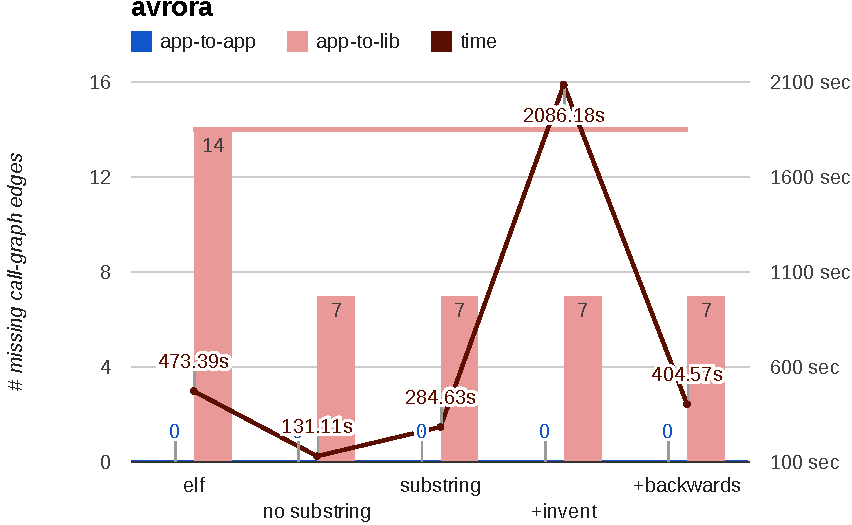
\includegraphics[width=\textwidth,height=0.2\textheight]{%
      figures/reflection/avrora-plain.pdf}
  \end{subfigure}
  ~
  \begin{subfigure}[t]{0.5\textwidth}
    \centering
    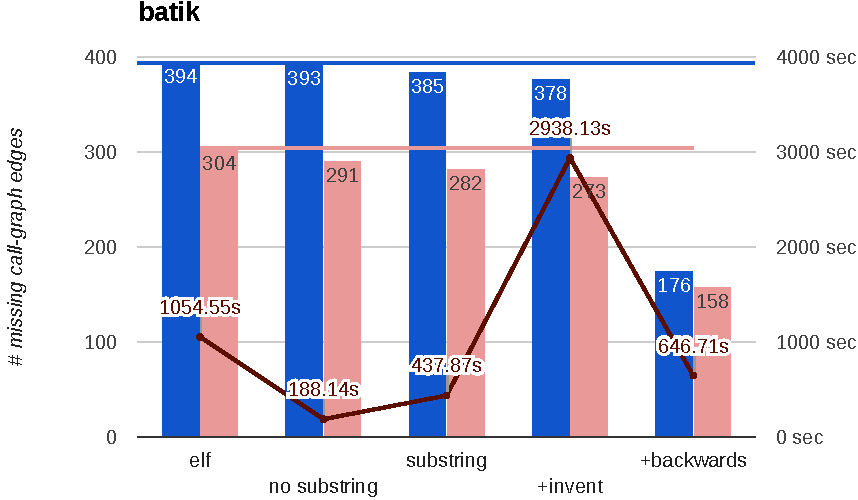
\includegraphics[width=\textwidth,height=0.2\textheight]{%
      figures/reflection/batik-plain.pdf}
  \end{subfigure}
  \\

  % 2nd row
  \begin{subfigure}[t]{0.5\textwidth}
    \centering
    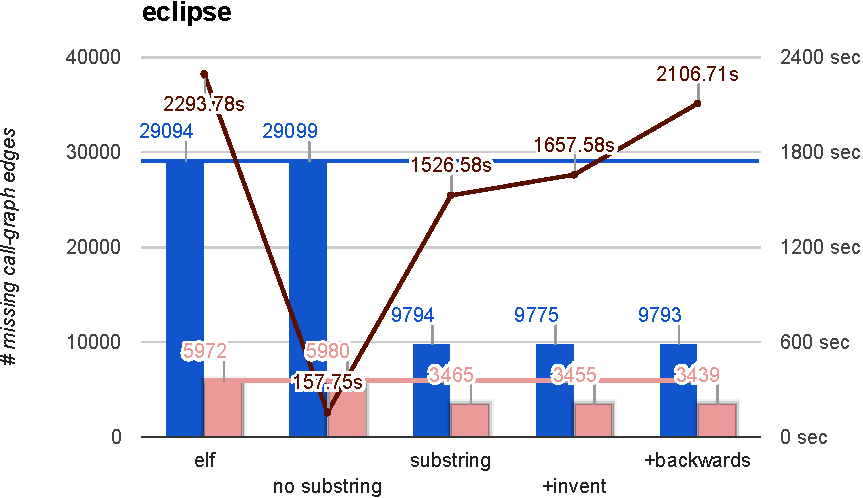
\includegraphics[width=\textwidth,height=0.2\textheight]{%
      figures/reflection/eclipse-plain.pdf}
  \end{subfigure}
  ~
  \begin{subfigure}[t]{0.5\textwidth}
    \centering
    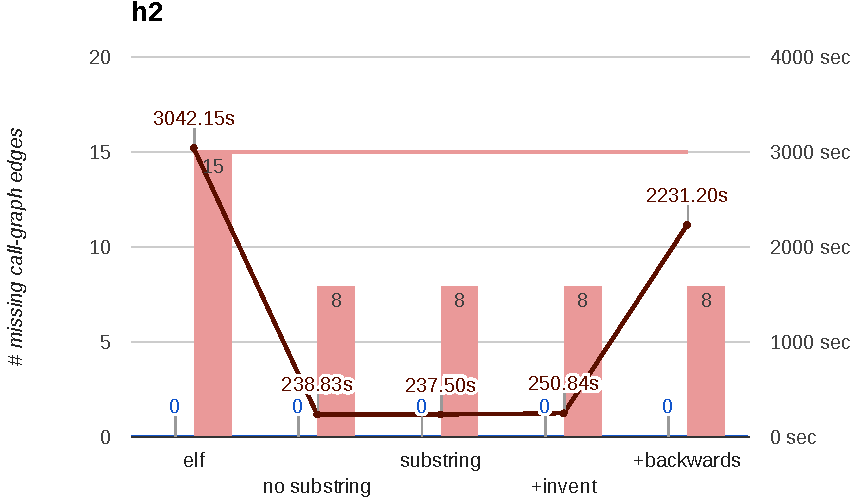
\includegraphics[width=\textwidth,height=0.2\textheight]{%
      figures/reflection/h2-plain.pdf}
  \end{subfigure}
  \\

  % 3rd row
  \begin{subfigure}[t]{0.5\textwidth}
    \centering
    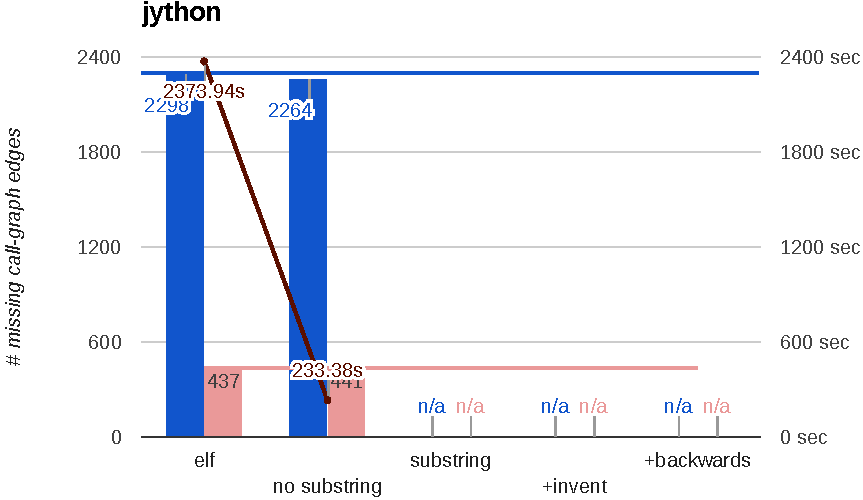
\includegraphics[width=\textwidth,height=0.2\textheight]{%
      figures/reflection/jython-plain.pdf}
  \end{subfigure}
  ~
  \begin{subfigure}[t]{0.5\textwidth}
    \centering
    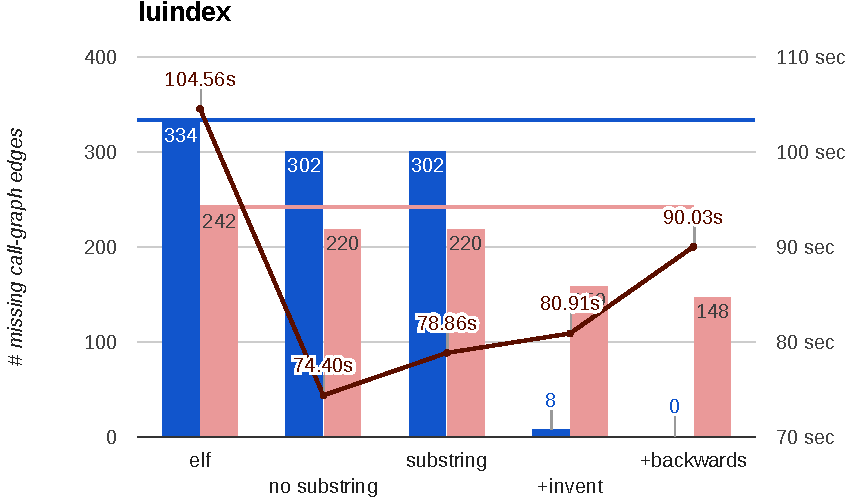
\includegraphics[width=\textwidth,height=0.2\textheight]{%
      figures/reflection/luindex-plain.pdf}
  \end{subfigure}
  \\

  % 4th row
  \begin{subfigure}[t]{0.5\textwidth}
    \centering
    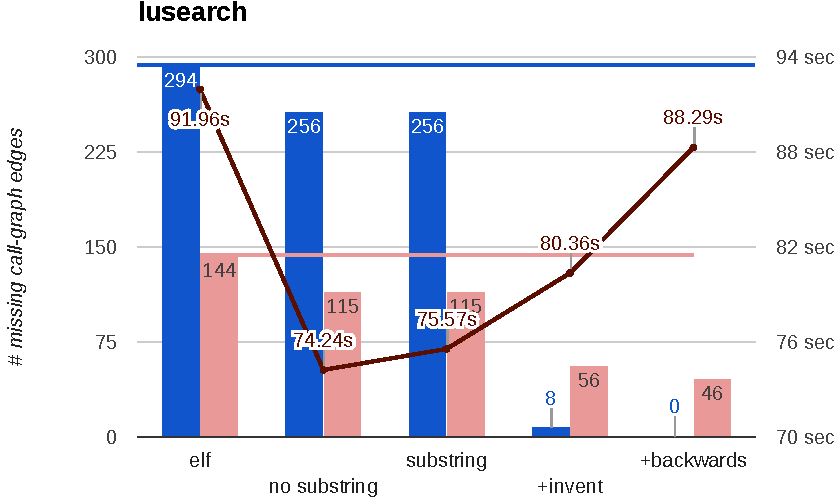
\includegraphics[width=\textwidth,height=0.2\textheight]{%
      figures/reflection/lusearch-plain.pdf}
  \end{subfigure}
  ~
  \begin{subfigure}[t]{0.5\textwidth}
    \centering
    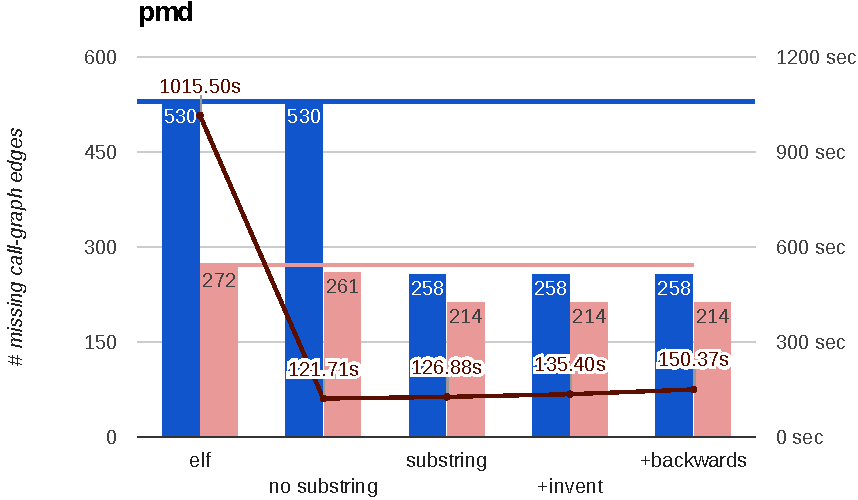
\includegraphics[width=\textwidth,height=0.2\textheight]{%
      figures/reflection/pmd-plain.pdf}
  \end{subfigure}
  \caption[Unsoundness metrics]{%
    Unsoundness metrics (two bars: missing call-graph edges app-to-app
    and app-to-lib) and analysis time (line) over the DaCapo
    benchmarks. \emph{Lower is better for all.} For missing bars
    (``n/a''), the analysis did not terminate in 90mins.}
\end{figure}
\begin{figure}\ContinuedFloat
  % 5th row
  \begin{subfigure}[t]{0.5\textwidth}
    \centering
    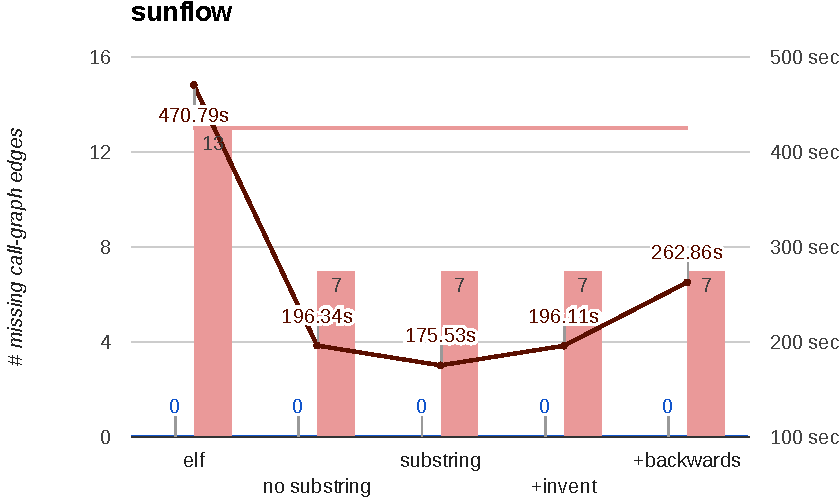
\includegraphics[width=\textwidth,height=0.2\textheight]{%
      figures/reflection/sunflow-plain.pdf}
  \end{subfigure}
  ~
  \begin{subfigure}[t]{0.5\textwidth}
    \centering
    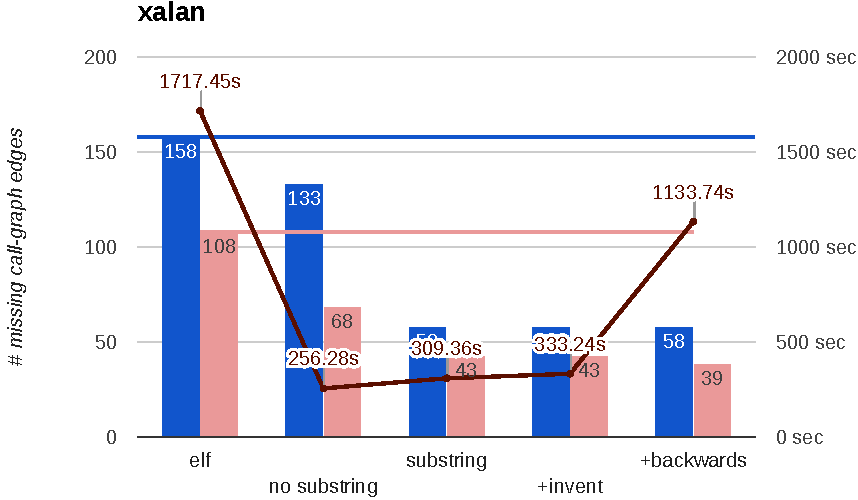
\includegraphics[width=\textwidth,height=0.2\textheight]{%
      figures/reflection/xalan-plain.pdf}
  \end{subfigure}


  % lusearch and sunflow could be left out

  \caption{Unsoundness metrics (cont.)}
  \label{reflection/fig:dacapo-bach}
\end{figure}

% \begin{figure}[t]
%   % \vspace{-1.5cm}
%   % \small
%   \scriptsize
%   \renewcommand{\tabcolsep}{1mm}
%   % \hspace*{-6mm}
%   \centering
%   \begin{tabular}{rrrrrrrrrrr}
%     \toprule
%     \textbf{Total Edges}
%     & \multicolumn{10}{c}{Benchmarks} \\
%     \cmidrule{2-11}
%     Setting & \centercell{avrora} & \centercell{batik} & \centercell{eclipse} & \centercell{h2} & \centercell{jython} & \centercell{luindex} & \centercell{lusearch} & \centercell{pmd} & \centercell{sunflow} & \centercell{xalan} \\
%     \midrule
%     elf & 19355 & 31602 & 10191 & 38252 & 19709 & 4547 & 4209 & 8544 & 4223 & 35918 \\
%     no substring & 19379 & 31708 & 9032 & 35538 & 20537 & 4676 & 4352 & 8592 & 4251 & 35221 \\
%     substring & 20591 & 35314 & 115967 & 38107 & n/a & 4682 & 4362 & 9533 & 4285 & 45160 \\
%     +invent & 26586 & 47303 & 116635 & 38162 & n/a & 5773 & 5266 & 9557 & 4319 & 45343 \\
%     +backwards & 20677 & 37013 & 117576 & 43952 & n/a & 6115 & 5587 & 9577 & 4407 & 63746 \\
%     \midrule
%     dynamic & 4165 & 8329 & 40026 & 4901 & 13583 & 3027 & 1845 & 4874 & 2215 & 6128 \\
%     \bottomrule
%   \end{tabular}
%   \footnotesize
%   \caption{Total static and dynamic call-graph edges for the DaCapo 9.12-Bach
%     benchmarks. These include only \emph{application-to-application}
%     and \emph{application-to-library} edges.}
%   \label{reflection/fig:total_static}
% \end{figure}

\begin{figure}[h]
  \renewcommand{\tabcolsep}{1.5mm}
  \centering
  \begin{tabular}{lr@{ \quad }rrrrr}
    \toprule
    \textbf{Total Edges} & & \multicolumn{5}{c}{Settings} \\
    \cmidrule(l){3-7}
    Benchmark & \emph{dynamic} & elf & no substring 
              & substring & +invent & +backwards
    \\
    \midrule
    avrora & 4165 & 19355 & 19379 & 20591 & 26586 & 20677 \\
    batik & 8329 & 31602 & 31708 & 35314 & 47303 & 37013 \\
    eclipse & 40026 & 10191 & 9032 & 115967 & 116635 & 117576 \\
    h2 & 4901 & 38252 & 35538 & 38107 & 38162 & 43952 \\
    jython & 13583 & 19709 & 20537 & n/a & n/a & n/a \\
    luindex & 3027 & 4547 & 4676 & 4682 & 5773 & 6115 \\
    lusearch & 1845 & 4209 & 4352 & 4362 & 5266 & 5587 \\
    pmd & 4874 & 8544 & 8592 & 9533 & 9557 & 9577 \\
    sunflow & 2215 & 4223 & 4251 & 4285 & 4319 & 4407 \\
    xalan & 6128 & 35918 & 35221 & 45160 & 45343 & 63746 \\
    \bottomrule
  \end{tabular}
  \caption[Total static and dynamic call-graph edges -- DaCapo
  9.12-Bach benchmarks]{Total static and dynamic call-graph edges for
    the DaCapo 9.12-Bach benchmarks. These include only
    \emph{application-to-application} and
    \emph{application-to-library} edges.}
  \label{reflection/fig:total_static}
\end{figure}


Figure~\ref{reflection/fig:dacapo-bach} plots the results of our experiments,
combining both analysis time and empirical unsoundness (in call-graph
edges). 
%We compare our techniques to the \textsc{Elf} system
%\cite{ecoop/LiTSX14}, which also attempts to improve reflection
%analysis for Java. 
Missing bars labeled ``n/a'' correspond to analyses
that did not terminate in 90mins (5400sec).
%
Each chart plots the
missing dynamic call-graph edges that are not discovered by the
corresponding static analysis. We use separate bars for the
\emph{application-to-application} and \emph{application-to-library}
edges.

% Library-to-library edges are also computed but they are not
% comparable in static vs. dynamic analysis due to native calls.
We consider only call-graph edges originating from application code,
since library classes contain a fair amount of non-analyzable native
methods.\footnote{Call-graph edges from the library are still fully
  statically analyzed, thus our experiments demonstrate scalability
  relative to large libraries. We just do not report
  library-originating edges (though they are computed within the time
  reported) since these only cloud the picture, due to native
  code. There is no easy way to compare library-to-library results to
  dynamic edges without manual filtering, which raises validity
  questions.}
% which \textsc{Doop} cannot analyze at all.
%
We also filter out some missing edges (i.e., consider them implicitly
covered), which involve the following methods:
\begin{itemize}
%[$\cdot$]
\item \emph{Class Initializers.}  \textsc{Doop} only models
%  Due to \textsc{Doop}'s modeling of
%  class initialization, no call-graph edges to and from \code{<clinit>}
%  methods are recorded. Instead, the analysis tracks down only
  \emph{which} subset of classes get initialized (without any
  information about where the initializer gets called from). We filter
  out edges to class initializer methods (i.e., \code{<clinit>}), if
  static analysis indicates that the class has been initialized.
\item \emph{Native.} Native code cannot be analyzed. However, some
  library reflection calls are wrappers for native methods (e.g.,
  \code{forName()} and \code{forName0()}). Edges to these methods are,
  thus, completely extraneous due to our special modeling
  of their effect.
\item \emph{Class Loader.} Method \code{loadClass()} is invoked by the
  VM when a class needs to be loaded and \code{checkPackageAccess()} is
  invoked right after loading.
  %% checkPackageAccess() is private and called automatically by the
  %% VM.
\item \emph{Synthetic.} Edges involving dynamically generated classes
  are impossible to obtain by reflection analysis alone, so we eliminate
  such instances.
\end{itemize}

%
% We filter out edges to implicit methods (static initializers,
% \code{loadClass()}) that are not statically modeled.

We show five techniques:

\begin{asparaenum}
\item \emph{Elf.} This is the \textsc{Elf} reflection analysis
  \cite{ecoop/LiTSX14}, which also attempts to improve reflection
  analysis for Java. 
%It serves as a baseline for the evaluation of the
%  four settings of our own analysis.
\item \emph{No substring.} Our reflection analysis, with 
  engineering enhancements over the original \textsc{Doop} framework,
  but no analysis of partial strings or their flow.
\item \emph{Substring.} The analysis integrates the substring and
  substring flow analysis of Section~\ref{reflection/sec:strings}.
\item \emph{+Invent.} This analysis integrates substring analysis as well as the
  object invention technique of Section~\ref{reflection/sec:invention}.
\item \emph{+Backwards.}\footnote{The \emph{+Backwards} and
    \emph{+Invent} techniques %are not comparable: they
    are both additions to the substring analysis, but neither includes
    the other.} This analysis integrates substring analysis as well as
  the back-propagation technique of
  Section~\ref{reflection/sec:back-propagation}.
\end{asparaenum}


It is important to note that, by design, our techniques
do not enhance the precision of an analysis, only its empirical
soundness.  Thus, the techniques
only find \emph{more} edges: they cover more of the
program. This improvement appears as a reduction in the figures
(``lower is better'') only because the number plotted is the
\emph{difference} in the missing edges compared to the dynamic
analysis.

Our research questions can now be answered:

\begin{description}
\item[RQ1: Do our techniques impact soundness?]
  As can be seen, our techniques substantially increase the soundness
  of the analysis.  In most benchmarks, more than half (to nearly all)
  of the missing \emph{application-to-application} edges are
  recovered by at least one technique. The
  \emph{application-to-library} missing edges also decreased, although
  not as much.  In fact, the \emph{eclipse} benchmark was hardly being
  analyzed in the past, since most of the dynamic call-graph was
  missing.

\item[RQ2: Do the techniques have reasonable running times?]
  Furthermore, although our approach emphasizes empirical soundness,
  it does not sacrifice scalability. All four of our settings are
  faster than \textsc{Elf} for almost all benchmarks. Aside from
  \emph{jython}, for which only the \textsc{Elf} and \emph{no
    substring} techniques are able to terminate before timeout, in
  all other cases \emph{substring} and at least one of \emph{+invent}
  or \emph{+backwards} outperformed \textsc{Elf}, while in 7-of-10
  benchmarks \emph{all} our techniques outperformed \textsc{Elf}.
  This is due to achieving scalability using the threshold techniques
  of Section~\ref{reflection/sec:throttling} instead of by sacrificing some
  empirical soundness, as \textsc{Elf} does. (A major design feature
  of \textsc{Elf} is that it explicitly avoids inferring reflection
  call targets when it cannot fully disambiguate them.)

%  In engineering terms, \textsc{Elf} is not comparable to our
%  approach, since it uses different underlying techniques. In contrast
%  to our emphasis on empirical soundness (e.g., with inter-procedural
%  backward flow of information from casts), \textsc{Elf} explicitly
%  avoids inferring reflection call targets when it cannot fully
%  disambiguate them. This achieves scalability but at the expense of
%  soundness. Instead, our experiments show that empirical soundness
%  can be achieved while our mechanisms of
%  Section~\ref{reflection/sec:throttling} manage to preserve scalability.

\item[RQ3: Do the techniques sacrifice precision?]
  For completeness, we also show a sanity-checking metric over
  our analyses. Empirical soundness could
  increase by computing a vastly imprecise call-graph. This is not the
  case for our techniques. Figure~\ref{reflection/fig:total_static} lists the
  total static and dynamic edges being computed. On average,
  \emph{+backwards} computes the most static edges (about $4.5$ times
  the number of dynamic edges). On the lower end of the spectrum lies
  \emph{no substring}, with a minimum of $3.4$ times the number of
  dynamic edges being computed.

\end{description}

% \item For 5-of-9 of the DaCapo 2006-10-MR2 benchmarks and for 3-of-9
%   or the DaCapo 9.12-Bach, there is no benefit to be gained by
%   advanced reflection analysis, because, even with baseline
%   techniques, our technique eliminates nearly all unsoundness.
%\item The combined techniques typically achieve quite high empirical
%  soundness.  For all 9 benchmarks from DaCapo 2006-10-MR2 and for
%  8-of-9 benchmarks of DaCapo 9.12-Bach, the recall of dynamic edges
%  for the most-sound technique is over 90\%. For 7-of-9 of the DaCapo
%  2006-10-MR2 and for 5-of-9 of DaCapo 9.12-Bach, the metric is at
%  over 97.5\%. The lowest recall (by at least 20\%) is exhibited by
%  the \emph{eclipse} benchmark, at 67\%. \emph{Eclipse}, however,
%  greatly benefits from our techniques: without substring analysis,
%  its recall drops to just 12\%. More representative benefits are
%  those of \emph{batik} and \emph{pmd v.4.2.5}, for which
%  techniques such as substring analysis and back-propagation lead to
%  discovering a total of over 300 extra real call-graph edges. (The
%  analysis did not terminate with the object invention technique for
%  \emph{batik}.)

% \item The run-time overhead of our analysis techniques ranges from the
%   un-noticeable to the substantial. Substring analysis typically
%   incurs a modest overhead (under 20\% for 14 of the 18 benchmarks)
%   but on occasion multiplies analysis times by large factors. The
%   eclipse benchmark is an extreme case, with analysis time increasing
%   tenfold when substring analysis is performed. However, as we saw
%   above, static analysis for eclipse misses most of the program's
%   behavior without substring analysis. The other two techniques
%   consistently add a 10-30\% overhead each, but with rare extreme
%   outliers, such as a sixfold overhead for back-propagation in the
%   case of \emph{xalan v.2.7.1}.

%\item Substring analysis yields the largest single improvement in
%  empirical soundness. Its recall increase is significant in 7 of the
%  18 benchmarks. Object invention makes a difference over that in 2
%  more benchmarks, and back-propagation improves (over substring
%  analysis) in 6 benchmarks. We do not plot the results of combining
%  object invention and back-propagation because for these benchmarks
%  (and for our current settings of parameters $c$ and $d$ from
%  Section~\ref{reflection/sec:throttling}) they hardly show a difference over
%  back-propagation alone, in either execution time or empirical
%  soundness.

%\item In terms of absolute numbers, each analysis technique typically
%  leads to discovering several tens of missing call-graph edges.

% \end{asparaenum}

%An interesting overall question is which of our techniques an analysis
%user should choose. As in most tunable analyses, 

In pragmatic terms, a user of our analysis should use flags to pick
the technique that yields more soundness without sacrificing
scalability, for the given input program. This is a familiar
approach---e.g., it also applies to picking the exact flavor and depth
of context-sensitivity.

%In summary, our techniques offer useful tradeoffs of soundness
%and scalability. They are  effective at improving our main
%soundness metric (recall of dynamic call-graph edges), and the cost is
%typically quite manageable. 

%Some outliers, in terms of extreme cost
%or extreme recall improvement are worthy of further study.


As a final note, the improved soundness due to the techniques
presented in this chapter supports our thesis statement:
%
\emph{the abstract model of memory is, indeed, improved by recovering
  implicit structural information via inference, primarily by tracking
  the use of types in the program.}
%
The use-based techniques leverage the way objects (returned by
reflective calls) are later used in the program: i.e., what types they
are cast to, what fields they access, and so on.  By inspecting the
use of reflective objects, these techniques are able to infer and
partly recover the objects' structure, which is not evident at the
site of their allocation, since the declared types involved in
reflective operations are too generic to accurately describe
them. Recovering such implicit structural information leads to a
better memory model; one that more faithfully abstracts the memory
that will be allocated by any actual execution.


\section{Summary}

In this chapter, we considered the problem of recovering structural
information for static analysis of Java. Structural information can be
lost due to inadequate reasoning of prior approaches about common
reflection patterns. Such reasoning often fails to identify the true
types of many memory allocations and leads to unsoundness. We
introduced the notion of empirical soundness, a metric that quantifies
how much of the actual dynamic behavior the static analysis covers.

Section~\ref{reflection/sec:intro} discusses the need for better
reflection handling in static analysis of Java programs and the
complications it poses to pointer analysis, specifically.
%
We give a simple model of a standard points-to analysis for Java, in
Section~\ref{reflection/sec:javapt}.
%
In Section~\ref{reflection/sec:model}, we add an inter-related
reflection analysis to this model, and then present the extensions
that constitute our approach in Section~\ref{reflection/soundiness}.
%
Intuitively, the traditional points-to part of the joint analysis
(Section~\ref{reflection/sec:javapt}) is responsible for computing how
heap objects flow intra- and inter-procedurally through the program,
while the added rules (of Sections \ref{reflection/sec:model} and
\ref{reflection/soundiness}) contribute only the reflection handling.
%
Finally, we evaluate our approach on the DaCapo 9.12-Bach suite, in
Section~\ref{reflection/sec:experiments}, in terms of empirical
soundness, by comparing against dynamic call-graphs.


\begin{comment}
Our treatment of reflection is
probably not the definitive solution to this problem of never-ending
complexity. Nevertheless, we believe it is an important step and it is
highly interesting (probably surprising to most experts) that
empirical soundness can be achieved without any external input for
widely used benchmark programs of significant complexity.

Other standard optimizations included allocating all reified fields,
objects, and constructors without context: they are immutable
objects. This was already done for reified classes.

The second challenge was to improve the scalability of
context-sensitive analyses under reflection. The natural first move
was to remove context-sensitivity from reflective method invocations
and reflective object allocations. Even the old code wasn't too good
at this: it didn't use the standard macros for creating new hcontexts
at reflective allocation sites, and at reflective call sites
(reflective virtual and reflective special) it just propagated the
context of the caller method. Instead, I now create a unique context
object (different from normal ones) and use that. This turns out to
lose virtually no precision (in any client-level metric), and in many
cases slightly *increased* precision (because even though it's just a
single calling context for all reflective calls, it cannot be confused
with normal calls to the same method). If one *wants*
context-sensitive reflection, then there is a preprocessor flag to
enable it (with the right macros for context creation, this time).


-tracking the flow of strings through StringBuffer and StringBuilder
objects In fact, this can be done in two modes: either by treating all
string factories as one object, or by distinguishing them.

-treating System and Application classes differently: it makes little
sense to access System classes via reflection. Their names, packages,
etc. are known to application code and to other system code. In
general, we care much more about application classes accessed via
reflection (which is a legitimate functionality for ultra-general
system code, as well as for other application code that tries or
adapts to configuration changes).

-tracking so many string constants (class/method/field names and
substrings of those) is extremely costly. Therefore there is the
ability to merge all of them into one constant (or, really, 3
representatives, since they are distinguished by type: one for all
class-name strings, one for all method-name strings, one for all
field-name strings). This restores scalability of the string object
var-points-to logic but risks losing scalability due to reflective
object flow tracking, in benchmarks that do use reflection seriously.

\end{comment}

\begin{comment}
\begin{figure}[h!t]
  \begin{math}
    \inferrule* [left=Class.forName\;]
    {\classForNameInstr[i]{c}{p}
      \\ \vptstr{p}{T}}
    {\vpt{c}{\reifiedclass{T}}}
  \end{math}
  \\

  \begin{math}
    \inferrule* [left=Class.newInstance\;]
    {\classNewInstanceInstr[i]{p}{c}
      \\ \vpt{c}{\reifiedclass{T}}}
    {\vpt{p}{o_{i,\tp{T}}}}
  \end{math}
  \\

  \begin{math}
    \inferrule* [left=Class.getMethod\;]
    {\classGetMethodInstr[i]{p}{c}{m}
      \\ \vpt{c}{\reifiedclass{T}}
      \\ \vptstr{m}{A::meth}
      \\\\ \lookup{T}{A::meth} = \_}
    {\vpt{p}{\reifiedmethod{A::meth}}}
  \end{math}
  \\

  \begin{math}
    \inferrule* [left=Method.invoke\;]
    {\methodInvokeInstr[i]{p}{m}{r}
      \\ \vpt{m}{\reifiedmethod{A::meth}}
      \\ \vpt{r}{o}
      \\ \alloctype{o} = \tp{T}
      \\\\ \lookup{T}{A::meth} = \code{B::meth}}
    {i \xrightarrow{calls} \code{B::meth}}
  \end{math}
  \\\\

  \begin{math}
    \inferrule* [left=String Builder\;]
    {\appendInstr[i]{b\(_1\)}{s}
      \\ \toStringInstr[j]{r}{b\(_2\)}
      \\ \vpt{b\(_1\)}{o_{b}}
      \\ \vpt{b\(_2\)}{o_{b}}
      \\\\ \alloctype{o_b} = \code{StringBuilder}
      \\ \vpt{s}{o_r}
      \\ \alloc{o_r} \in \reflObjects}
    {\vpt{r}{o_r}}
  \end{math}
  \\

  \begin{math}
    \inferrule* [left=Class Substr\;]
    {\classForNameInstr[i]{c}{p}
      \\ \vpt{p}{str}
      \\ \javastring{\ldots} + \alloc{str} + \javastring{\ldots} = \javastring{T}}
    {\vpt{c}{\reifiedclass{T}}}
  \end{math}
  \\\\

  \begin{math}
    \inferrule* [left=Class.forName\(^{+}\)\;]
    {\classForNameInstr[i]{c}{p}}
    {\vpt{c}{\reifiedclass{i,*}}}
  \end{math}
  \\

  \begin{math}
    \inferrule* [left=Class.newInstance\(^{+}\)\;]
    {\classNewInstanceInstr[j]{p}{c}
      \\ \vpt{c}{\reifiedclass{i,*}}}
    {\vpt{p}{o_{i,\tp{*}}}}
  \end{math}
  \\

  \begin{math}
    \inferrule* [left=Cast\;]
    {\classForNameInstr[i]{c}{x}
      \\ \castinstr[j]{p}{T}{q}
      \\ \subtypeof{T'}{T}
      \\ \vpt{q}{o_{i,\tp{*}}}}
    {\vpt{c}{\reifiedclass{T'}}}
  \end{math}
  \\\\

  \begin{math}
    \inferrule* [left=Class.newInstance\(^{++}\)\;]
    {\classNewInstanceInstr[i]{p}{c}}
    {\vpt{p}{m_{i}}}
  \end{math}
  \quad
  \begin{math}
    \inferrule* [left=Invent\;]
    {\castinstr[j]{p}{T}{q}
      \\ \vpt{q}{m_{i}}}
    {\vpt{p}{m_{i,\tp{T}}}}
  \end{math}
  \caption{Inference Rules}
  \label{reflection/fig/rules}
\end{figure}

\end{comment}


%%% Local Variables:
%%% mode: latex
%%% TeX-master: "../thesis"
%%% End:


\chapter[Class Hierarchy Complementation for Java]{%
  Class Hierarchy Complementation: \NoCaseChange{\\}
  Soundly Completing a Partial Type Graph}
\label{chapter:complementation}
\epigraph{What in God's holy name are you blathering
  about?}{\textit{The Big Lebowski}}

In the previous chapter, we examined the problems caused by Java's
reflection and presented a reflection analysis, integrated into a
standard points-to analysis, that recovers structural information for
reflective objects. In this chapter, we will continue to examine the
problem of lost memory structure in Java, yet in a completely
different context: that of \emph{partial Java programs}.

As stated in Chapter~\ref{chapter:intro}, analyzing partial programs
is crucial for Java, whose dynamic class loading allows JAR files to
depend on an abundance of external libraries, even though only a
subset of them will be required at runtime---in any possible
execution. The primary challenge in analyzing partial Java programs
concerns the implied type constraints in existing code, and their
repercussions on the type hierarchy.
%-------------------------------------------------------------------------------
% Prior abstract
%-------------------------------------------------------------------------------
This leads to the more generic problem of class hierarchy
complementation: given a partially known hierarchy of classes together
with subtyping constraints (``A has to be a transitive subtype of B'')
complete the hierarchy so that it satisfies all constraints.

The problem has immediate practical application to the analysis of
partial programs---e.g., it arises in the process of providing a sound
handling of ``phantom classes'' in the Soot program analysis
framework. We provide algorithms to solve the hierarchy
complementation problem in the single inheritance and multiple
inheritance settings.
% We show that class
% hierarchy complementation is NP-complete for multiple
%inheritance/subtyping while there is a polynomial algorithm for single
% subtyping hierarchies.
We also show that the problem in a language such as Java, with single
inheritance but multiple subtyping and distinguished class
vs. interface types, can be decomposed into separate single- and
multiple-subtyping instances.  We implement our algorithms in a tool,
JPhantom, which complements partial Java bytecode programs so that the
result is guaranteed to satisfy the Java verifier requirements. In a
sense, JPhantom aims to recover structural information for phantom
classes, via inference, by tracking their use in existing
code. JPhantom is highly scalable and runs in mere seconds even for
large input applications and complex constraints (with a maximum of
14s for a 19MB binary).

%Static whole-program analysis requires the availability of every class
%transitively referenced in a program, even if it is never used. For
%instance, trying to analyze a program P that uses a small part of a
%third-party library L also requires the full code of any library L'
%that different parts of L may reference---the fact that L' is not
%necessary for P cannot be determined before the analysis of P is
%performed. This is a oft-encountered practical challenge, motivating
%mechanisms such as the ``phantom class'' facility in the well-known
%Soot analysis framework for Java.
%
%To address this challenge in full generality we define the problem of
%``program complementation'': given a partial program we seek to
%provide definitions for its missing parts so that the ``complement''
%satisfies all static and dynamic typing requirements induced by the
%code under analysis. This requires satisfying constraints relative to
%methods and fields of the missing classes, as well as subtyping
%constraints and constraints on whether a missing type has to be a
%class or interface. We formulate the problem systematically and offer
%an algorithm that produces solutions for the resulting constraints.
%The result is the articulation of a novel typing problem in the OO
%context, as well as a tool of practical interest. We show that we
%produce practical complements of significant size in a few seconds
%and, in this way, allow the analysis of previously un-analyzable
%partial programs.


%-------------------------------------------------------------------------------
% Introduction
%-------------------------------------------------------------------------------

\section{Overview of Partial Type Hierarchy and Program Complementation}
\label{hiercomp/intro}

Whole-program static analysis is essential for clients that require
high-precision
%in analysis results
and a deeper understanding of program behavior. Modern applications of
program analysis, such as large scale refactoring tools
\cite{journals/software/Dig11}, race and deadlock detectors
\cite{pldi/NaikAW06}, and security vulnerability detectors
\cite{sigsoft/MadsenLF13,uss/GuarnieriL09}, are virtually
inconceivable without whole-program analysis.

For whole-program analysis to become truly practical, however, it
needs to overcome several real-world challenges. One of the somewhat
surprising real-world observations is that whole-program analysis
requires the availability of much more than the ``whole program''.
The analysis needs an overapproximation of what constitutes the
program. Furthermore, this overapproximation is not merely
what the analysis computes to be the ``whole program'' after it
has completed executing. Instead, the overapproximation needs to be
as conservative as required by any intermediate step of the analysis,
which has not yet been able to tell, for instance, that some method
is never called.

Consider the example of trying to analyze a program $P$ that uses a
third-party library $L$. Program $P$ will likely only need small parts
of $L$.  However, other, entirely separate, parts of $L$ may make use
of a second library, $L'$.  It is typically not possible to analyze
$P$ with a whole program analysis framework without also supplying the
code not just for $L$ but also for $L'$, which is an unreasonable
burden. In modern languages and runtime systems, $L'$ is usually not
necessary in order to either compile $P$ or run it under any
input. The problem is exacerbated in the current era of large-scale
library reuse.  In fact, it is often the case that the user is not
even aware of the existence of $L'$ until trying to analyze $P$.

Unsurprisingly, the issue has arisen before, in different guises.  The
FAQ document\footnote{http://www.sable.mcgill.ca/soot/faq.html} of the
well-known Soot framework for Java
analysis \cite{vall99soot,valleerai00optimizing} contains the
question:

\vspace{-1mm}
\begin{quote}
  \emph{How do I modify the code in order to enable soot to continue
    loading a class even if it doesn't find some of it[s] references?
    Can I create a dummy soot class so it can continue with the load?
    How?}
\end{quote}

\noindent This frequently asked question does not lead to a
solution. The answer provided is:
\begin{quote}
  \emph{You can try -use-phantom-refs but often that does not work
    because not all analyses can cope with such references. The best
    way to cope with the problem is to find the missing code and
    provide it to Soot.}
\end{quote}

The ``phantom refs'' facility of Soot, referenced in the above answer,
attempts to model missing classes (\emph{phantom classes}) by
providing dummy implementations of their methods referenced in the
program under analysis. However, there is no guarantee that the
modeling is in any way sound, i.e., that it satisfies the well-formedness
requirements that the rest of the program imposes on the phantom
class.

Our research consists precisely of addressing the above need in full
generality. \emph{Given a set of Java class and interface definitions,
  in bytecode form, we compute a ``program complement'', i.e.,
  skeletal versions of any referenced missing classes and interfaces
  so that the combined result constitutes verifiable Java bytecode.}
Our solution to this practical problem has two parts:

\begin{asparaitem}[$\cdot$]
\item A \emph{program analysis} part, requiring analysis of bytecode
  and techniques similar to those employed by the Java verifier and
  Java decompilers. This analysis computes constraints involving the
  missing types. For instance, if a variable of a certain type $C$ is
  direct-assigned to a variable of a type $S$, then $C$ must be a
  subtype of $S$.
  % , as well as constraints on members (e.g., we may know from
  % available bytecode that a missing class has a method with a given
  % signature)
\item An \emph{algorithmic} part, solving a novel typing problem, which we call
  the \emph{class hierarchy complementation}, or
  simply \emph{hierarchy complementation}, problem. The problem
  consists of computing a type hierarchy that satisfies a set of
  subtyping constraints \emph{without} changing the direct parents of
  known types.
\end{asparaitem}


%We model all requirements on missing classes or interfaces
%(which we call ``phantom types'', alluding to the Soot terminology) as
%a set of typing constraints.

The algorithmic part of our solution, i.e., solving the hierarchy
complementation problem, constitutes the main novelty of our
approach. The problem appears to be fundamental, and even of a certain
interest in purely graph-theoretic terms. For a representative special
case, consider an object-oriented language with multiple inheritance
(or, equivalently, an interface-only hierarchy in Java or
C\#).\footnote{We avoid the terms ``subclassing'' or ``inheritance''
  as synonyms for ``direct subtyping'' to prevent confusion with other
  connotations of these terms. In our context, we only care about the
  concept of subtyping, i.e., of a (monomorphic) type as a special
  case of another. Subtyping can be direct (e.g., when a Java class is
  declared to ``extend'' another or ``implement'' an interface) or
  indirect, i.e., transitive. We do, however, use the compound terms
  ``single inheritance'' and ``multiple inheritance'' as they are more
  common in the classification of languages than ``single subtyping''
  and ``multiple subtyping''.}  A partial hierarchy, augmented with
constraints, can be represented as a graph, as shown in
Figure~\ref{hiercomp/fig:ex0:problem}. The known part of the hierarchy is shown
as double circles and solid edges. Unknown (i.e., missing) classes are
shown as single circles. Dashed edges represent subtyping constraints,
i.e., indirect subtyping relations that have to hold in the resulting
hierarchy. In graph-theoretic terms, a dashed edge means that there is
a path in the solution between the two endpoints. For instance, the
dashed edge from $C$ to $D$ in Figure~\ref{hiercomp/fig:ex0:problem} means that
the unknown part of the class hierarchy has a path from $C$ to
$D$. This path cannot be a direct edge from $C$ to $D$, however: $C$
is a known class, so the set of its supertypes is fixed.

\begin{figure}
  \begin{minipage}[b]{.5\linewidth}
    \centering
    \includegraphics[scale=0.6]{figures/complementation/cgraph2.pdf}
    \subcaption{Constraint Graph}\label{hiercomp/fig:ex0:problem}
  \end{minipage}
  \begin{minipage}[b]{.5\linewidth}
    \centering
    \includegraphics[scale=0.6]{figures/complementation/cgraph2-solution.pdf}
    \subcaption{Solution}\label{hiercomp/fig:ex0:solution}
  \end{minipage}
  \caption[Example of constraints in a multiple inheritance setting]{%
    Example of constraints in a multiple inheritance
    setting. Double-circles signify known classes, single circles
    signify unknown classes. Solid edges (``known edges'') signify
    direct subtyping, dashed edges signify transitive subtyping.}
  \label{hiercomp/fig:ex0}
\end{figure}

In order to solve the above problem instance, we need to compute a
directed acyclic graph (DAG) over the same nodes,\footnote{Inventing
extra nodes does not contribute to a solution in this problem.} so
that it preserves all known nodes and edges, and adds edges \emph{only
to unknown nodes} so that all dashed-edge constraints are
satisfied. That is, the solution will not contain dashed edges
(indirect subtyping relationships), but every dashed edge in the input
will have a matching directed path in the solution
graph. Figure~\ref{hiercomp/fig:ex0:solution} shows one such possible solution.
As can be seen, solving the constraints (or determining that they are
unsatisfiable) is not trivial. In this example, any solution has to
include an edge from $B$ to $E$, for reasons that are not immediately
apparent. Accordingly, if we change the input of
Figure~\ref{hiercomp/fig:ex0:problem} to include an edge from $E$ to $B$, then
the constraints are not satisfiable---any attempted solution
introduces a cycle. The essence of the algorithmic difficulty of the
problem (compared to, say, a simple topological sort) is that we
cannot add extra direct parents to known classes $A$ and $C$---any
subtyping constraints over these types have to be satisfied via
existing parent types. This corresponds directly to our high-level
program requirement: we want to compute definitions for the missing
types only, without changing existing code.

% We show that computing whether such a DAG exists is an
% NP-complete problem, for the case of multiple subtyping.

For a language with single inheritance, the problem is similar, with
one difference: the solution needs to be a tree instead of a DAG. (Of
course, the input in Figure~\ref{hiercomp/fig:ex0:problem} already violates the
tree property since it contains known nodes with multiple known
parents.) We offer an algorithm that solves the problem by
either detecting unsatisfiability or always ordering the nodes in a
tree that respects all constraints.

%\footnote{Although this is true only because we are accepting any
%legal bytecode as input. As we discuss later, if we assume that the
%input is produced by following specific compiler conventions
%then...}

The practical version of the hierarchy complementation problem is more
complex. Mainstream OO languages often distinguish between classes and
interfaces and only allow single direct subtyping among classes and
multiple direct subtyping from a class/interface to an interface---a
combination often called ``single-inheritance, multiple
subtyping''. In this case, the graph representation of the problem is
less intuitive. Consider Figure~\ref{hiercomp/fig:real-example:problem} that
gives a problem instance. (A possible solution for these constraints
is in Figure~\ref{hiercomp/fig:real-example:solution}, but is given purely for
reference, as it is not central to our discussion.) There are now
several node types: classes, interfaces (both known and unknown), as
well as undetermined nodes. There are also more implicit constraints
on them: classes can only have an edge to one other class, interfaces
can only have edges to other interfaces.  The latter constraint, for
instance, forces $D$ to be an interface and $H$ to be a class. Thus, we
see that the full version of the problem requires additional
reasoning. We show that such reasoning can be performed as a
pre-processing step. The problem can be subsequently broken up into
two separate instances of the aforementioned single- and
multiple-inheritance versions of hierarchy complementation.

%merely refines locally the algorithms for solving the
%problem versions for multiple inheritance and

\begin{figure}[ht]
  \begin{minipage}[b]{.5\linewidth}
    \centering
    \includegraphics[scale=0.6]{figures/complementation/cgraph3.pdf}
    \subcaption{Constraint Graph}\label{hiercomp/fig:real-example:problem}
  \end{minipage}
  \begin{minipage}[b]{.5\linewidth}
    \centering
    \includegraphics[scale=0.6]{figures/complementation/cgraph3-solution.pdf}
    \subcaption{Solution}\label{hiercomp/fig:real-example:solution}
  \end{minipage}
  \caption[Example of full-Java constraint graph]{Example of full-Java
    constraint graph. Double circles denote known classes/interfaces,
    whose outgoing edges in the solution are already determined (solid
    input edges). White nodes are classes, black nodes are interfaces,
    grey nodes are unknown types that are initially undetermined
    (i.e., the input does not explicitly identify them as classes or
    interfaces, although constraint reasoning may do so later).}
  \label{hiercomp/fig:real-example}
\end{figure}



% Subsequently, we offer an algorithm for
% solving program complementation constraints. We implement our solution
% for Java, at the bytecode level. Our resulting tool accepts as
% input a set of Java bytecode files and produces a jar file with
% appropriate definitions of all phantom types.

%% The well-formedness guarantee of our solution to the program
%% complementation problem is that we produce classes that could have
%% been produced by the front-end Java compiler (javac) for \emph{some}
%% definition of phantom classes. This offers no guarantee that the
%% resulting original program + complement will not exhibit dynamic type
%% errors, but such a guarantee is not required: the assumption is that
%% phantom classes are indeed \emph{not used} in a meaningful way, and
%% all we want is for them to be consistent with the rest of the
%% program. For instance, a key consistency property of our solution
%% relative to the Soot phantom class treatment is that we respect
%% subtyping: if a subtyping relationship involving a phantom class
%% (or interface) can be inferred from the code then it is satisfied
%% in the complement that we output.

% To see why the problem has interesting depth and complexity, consider
% a simple fragment of Java bytecode and the constraints it
% induces. Our convention throughout this chapter is that single-letter
% class names at the lower end of the alphabet (\code{A}, \code{B},
% ...)  correspond to known types, while class names at the high end
% of the alphabet (\code{X}, \code{Y}, \code{Z}) denote phantom types.
% We present bytecode in a slightly condensed form, to make clear what
% method names or type names are referenced in every instruction.
%
% \begin{smallnolinecode}
% \begin{verbatim}
% public void foo(X, Y);
%  0: aload_2     // load on stack 2nd argument (of type Y)
%  1: aload_1     // load on stack 1st argument (of type X)
%  2: invokevirtual X.bar:(LA;)LZ; //method 'Z bar(A)' in X
%  3: checkcast B // cast the result of the call to B
%  ...
% \end{verbatim}
% \end{smallnolinecode}
%
% Although the above fragment is merely four bytecode instructions
% long, it induces several interesting constraints for our phantom
% types \code{X}, \code{Y}, and \code{Z}:
%
% \begin{bullets}
% \item \code{X} has to support a method \code{bar} accepting an
%   argument of type \code{A} and returning a value of type \code{Z}.
%
% \item \code{Y} has to be a subtype of \code{A}, since an actual
%   argument of declared type \code{Y} is passed to \code{bar}, which
%   has a formal parameter of type \code{A}. This constraint also
%   means that if \code{A} is known to be a class (and not an
%   interface) then \code{Y} is also a class.
%
% \item \code{Z} is either a subtype of \code{B} or a supertype of
%   \code{B}.  The reason is that we have a cast from a reference of
%   type \code{Z} to one of type \code{B} and our well-formedness
%   requirements dictate that no dynamic type error (class cast
%   exception) be produced by such a cast. A naive view would suggest
%   that the real constraint induced by the cast is that \code{Z} be a
%   supertype of \code{B} (since the existence of a dynamic cast check
%   implies a narrowing conversion) but the bytecode may elide any
%   number of intermediate casts that existed in the source code. For
%   instance, the source code may have cast the return value of
%   \code{bar} to \code{java.lang.Object} (a cast that is always safe
%   and thus disappears in the bytecode) before casting it to
%   \code{B}. Thus, the real constraint is that \code{Z} (which is
%   only the static type of the reference, and therefore a supertype
%   of the dynamic type of the object) is either a subtype or
%   supertype of \code{B}.
% \end{bullets}
%
% Our approach will create skeletal versions of \code{X}, \code{Y},
% and \code{Z} so that all the above requirements are
% satisfied. Clearly, there can be unsatisfiable instances of the
% above constraints (e.g., cyclic subtyping requirements), and these
% are detected by our algorithm. However, unsatisfiable constraints
% cannot arise in real-world instances of the problem, unless parts of
% the code have changed without recompiling other, dependent parts.

In brief, the contributions of our work are as follows:

\begin{itemize}[--]
\item We introduce a new typing problem, motivated by real-world needs
  for whole program analysis. To our knowledge, the hierarchy
  complementation problem has not been studied before, in any context.
\item We produce algorithms that solve the problem in three different
  settings: single inheritance, multiple inheritance, and mixture of
  the two, as in Java or C\#.
%  For a single inheritance setting, we
%  offer a simple algorithm, possibly of wider applicability to other
%  domains (e.g., partially-ordered sets for which the concept of
%  ``direct predecessor'' needs to be distinguished from merely ``in
%  order''). Based on similar insights, we adapt the algorithm to a
%  multiple inheritance setting.
%  For the practical setting of a single-inheritance,
%  multiple-subtyping language, we offer an algorithm that decomposes
%  the problem into the previous two versions.
%, and also prove
% that the problem is NP-complete.
%  we offer an algorithm
%  that has exponential complexity in the worst case.
\item We implement our algorithms in JPhantom: a practical tool for
  Java program complementation that addresses the soundness
  shortcomings of previous Java ``phantom class'' approaches. We show
  that JPhantom scales well and takes only a few seconds to process
  even large benchmarks with complex constraints---e.g., less than
  6sec for a 3.2MB binary that induces more than 100 constraints.
%, encountering no exponential complexity
%  in practice.
\item We discuss the problem of hierarchy complementation in more
  general settings. The simplicity of our approach is a result of only
  assuming (for the input) and satisfying (for the output) the fairly
  weak Java bytecode requirements. We show that the problem becomes
  harder at the level of the type system for the source language.
\end{itemize}


%-------------------------------------------------------------------------------
% Motivation
%-------------------------------------------------------------------------------

% In the next sections we detail
\section{Motivation and Practical Setting}

We next discuss the practical setting that gives rise to the hierarchy
complementation problem.

Our interest in hierarchy complementation arose from efforts to
complement existing Java bytecode in a way that satisfies the
soundness guarantees of the Java verifier. Consider a small fragment
of known Java bytecode and the constraints it induces over unknown
types. (We present bytecode in a slightly condensed form, to make
clear what method names or type names are referenced in every
instruction.) In this code, classes \code{A} and \code{B} are
available, while types \code{X}, \code{Y}, and \code{Z} are phantom,
i.e., their definition is missing.

\begin{bytecode}
  public void foo(X, Y)
  0: aload_2     // load on stack 2nd argument (of type Y)
  1: aload_1     // load on stack 1st argument (of type X)
  2: invokevirtual X.bar:(LA;)LZ; // method 'Z bar(A)' in X
  3: invokevirtual B.baz:()V;     // method 'void baz()' in B
   ...
\end{bytecode}

The instructions of this fragment induce several constraints for our phantom
types. For instance:

\begin{itemize}[--]
\item \code{X} has to be a class (and not an interface) since it
  contains a method called via the \code{invokevirtual} bytecode
  instruction.
\item \code{X} has to support a method \code{bar} accepting an
  argument of type \code{A} and returning a value of type \code{Z}.
\item \code{Y} has to be a subtype of \code{A}, since an actual
  argument of declared type \code{Y} is passed to \code{bar}, which
  has a formal parameter of type \code{A}. This constraint also means
  that if \code{A} is known to be a class (and not an interface) then
  \code{Y} is also a class.
\item \code{Z} has to be a subtype of \code{B}, since a method of
  \code{B} is invoked on an object of declared type \code{Z} (returned
  on top of the stack by the earlier invocation).
\end{itemize}

The goal of our JPhantom tool is to satisfy all such constraints and
generate definitions of phantom types \code{X}, \code{Y}, and \code{Z}
that are compatible with the bytecode that is available to the tool
(i.e., exists in known classes). Compatibility with existing bytecode
is defined as satisfying the requirements of the Java verifier, which
concern type well-formedness.

Of these constraints, the hardest to satisfy are those involving
subtyping.  Constraints on members (e.g., \code{X} has to contain a
``\code{Z bar(A)}'') are easy to satisfy by just adding type-correct
dummy members to the generated classes. This means that the problem in
the core of JPhantom is solving the class hierarchy complementation
problem, as presented in the introduction and defined rigorously in
later sections. The binding of the problem to practical circumstances
deserves some discussion, however.

First, note that, in our setting of the problem, we explicitly
disallow modification of known code, e.g., in order to remove
dependencies, or to add a supertype or a member to it. Such
modifications would have a cascading effect and make it hard to argue
about what properties are really preserved. Additionally, we do not
assume any restrictions on the input, other than the well-formedness
condition of being legal Java bytecode (according to the
verifier). Strictly speaking, our well-formedness condition for the
input is defined as follows: \emph{a legal input is bytecode that can
  be complemented (by only adding extra class and interface
  definitions) so that it passes the Java verifier}. Note that this
well-formedness condition does not depend on the program complement
that our approach produces: an input is legal if there is \emph{some}
complement for it, not necessarily the one that JPhantom computes.

%%% We later use this. Better not emphasize it.
%Notably, this well-formedness condition does
%not assume that known classes have known superclasses---e.g.,
%Figure~\ref{hiercomp/fig:real-example:problem} offered an instance where a
%superclass was a phantom type. Of course, an actual usage setting of
%JPhantom can impose this or other restrictions on the input.

% There
%are several good reasons for this decision: First, modification of
%existing code would likely
%-we cannot modify existing code. E.g., adding a supertype induces
%constraints that are not satisfied (e.g., an interface method may not be
%implemented).

A final interesting point concerns the practical impact of the
JPhantom soundness condition. For most program analyses, omitting
parts of the code introduces unsoundness, if we make no other
assumptions about the program or the omitted part. E.g., it is
impossible to always soundly compute points-to information, or
may-happen-in-parallel information when part of the program is
missing. Therefore, guaranteed soundness for all clients is inherently
unachievable for \emph{any} partial program analysis approach. The
practical reality is that there is a large need for facilities for
handling partial programs. For instance, the Soot phantom class
machinery has been one of the most common sources of discussion and
questions on the Soot support lists, and it has been a central part of
several Soot revisions.\footnote{Even the most recent Soot release,
2.5.0, lists improved support for phantom classes and excluding
methods from an analysis as one of the major changes in the release
notes.} The only ``correctness condition'' that Soot phantom class
support is trying to achieve, however, is the low-level ``the analyzer
should not crash''.

Given the practical interest for the solution of a worst-case
unsolvable problem, we believe that our soundness guarantee makes a
valuable contribution: it is much better to analyze a partial program
in a way such that the Java verifier requirements (for type-level
well-formedness) are satisfied than to ignore any correctness
considerations, as past approaches do.

% unsatisfiable constraints cannot arise in
%real-world instances of the problem, unless parts of the code have
%changed without recompiling other, dependent parts.


%-------------------------------------------------------------------------------
% Multiple Inheritance
%-------------------------------------------------------------------------------

\section{Hierarchy Complementation for Multiple Inheritance}
\label{hiercomp/multiple}

We begin with a modeling of the hierarchy complementation problem in
the setting of multiple inheritance. This means that every class in our
output can have multiple parents.

%% Formalization

We can model our problem as a graph problem. Our input is a directed
graph $G = (V,E)$, with two disjoint sets of nodes $V = V_{known} \disjunion
V_{phantom}$ and two disjoint sets of edges $E = E_{direct} \disjunion
E_{path}$, where $E_{direct} \subseteq V_{known} \times V$ (i.e.,
direct edges have to originate from known nodes---the converse is not
true, as known nodes can be inferred to subtype unknown ones due to
assignment instructions in the bytecode). The set of nodes $V$ is a
set of types, while the set of edges $E$ corresponds to our subtyping
constraints. That is, an edge $(v_s,v_t)$ encodes the constraint $v_s
<: v_t$. The $E_{direct}$ subset encodes the direct-subtype
constraints. The output of our algorithm should be a \emph{DAG} (with
edges from children to their parents), $G_D = (V,E')$, such that:
\begin{enumerate}
\item
  $\forall v_s \in V_{known}: (v_s,v_t) \in E' \Leftrightarrow (v_s,
  v_t) \in E_{direct}$ (i.e., all direct edges from known nodes are
  preserved and no new ones are added to such nodes)
\item $(v_s,v_t) \in E_{path} \Rightarrow$ there is a path from $v_s$
  to $v_t$ in $G_D$
\end{enumerate}

% Again, we could decouple path-edges from direct-edges by introducing
% the input and output mappings, $f_i:V_{known} \rightarrow 2^V$,
% $f_o:V \rightarrow 2^V$. In both cases, these two mappings map a
% type (key) to its \emph{set} of outgoing edges (value). This way,
% $G_C = (V,E)$ will only contain path-edges such that
% $\forall (x_1,x_n) \in E :$ there must exist a path
% $(x_1,x_2,\ldots,x_n) \text{ in } G_D$ (second
% constraint). Additionally, as in the single inheritance case, we
% must ensure that $\forall c \in V_{known}: f_o[c] = f_i[c]$ (first
% constraint).

Note that our only limiting constraint here is that we cannot have
cycles in the resulting hierarchy. Moreover, since each type may have
multiple supertypes in this setting, a directed acyclic graph is
fitting as our intended output.

%% Phantom-only case

In contrast to the general case, the problem is trivial if we have a
phantom-only input, i.e., if we ignore $V_{known}$ and
$E_{direct}$. It suffices to employ a cycle-detection algorithm,
and---if no cycles are present---return the input constraint graph as
our solution: all path edges can become direct subtyping edges. If our
input graph contains a cycle, then our problem is unsolvable.  If
not, our solution would probably contain some redundant edges (i.e.,
edges connecting nodes that are already connected by another path)
that we could prune to minimize our output. In either case, our
solution would be valid w.r.t. our constraints.

% Optionally, we could prune some edges from our solution without
% breaking any constraints, to minimize the output of our algorithm
% for practical purposes. Algorithm~\ref{hiercomp/alg:multiple:simple} performs
% such an optimization, by first computing a transitive closure of the
% constraints and then removing redundant edges, whose target can be
% reached from another path.

%% Projection Sets

The problem becomes much more interesting when we take $V_{known}$
into account. The source of the difficulty is the combination of cycle
detection with nodes whose outgoing edge set cannot be extended.
Consider first the pattern of Figure~\ref{hiercomp/fig:choice}.

\begin{figure}[ht]
  \centering \includegraphics[scale = 0.6]{figures/complementation/cgraph-min.pdf}
  \caption[Multiple Inheritance Constraint]{In any solution of these
    constraints, either $B$ or $C$ or $D$ have to be ordered below
    $E$, since no new outgoing edges can be added to $A$ and the path
    constraint to $E$ needs to be satisfied.}
  \label{hiercomp/fig:choice}
\end{figure}

This pattern is a basic instance of interesting reasoning in the case of
multiple inheritance. We have $A \in V_{known}$ such that $(A,B),
(A,C), (A,D) \in E_{direct}$ and $(A,E) \in E_{path}$. We cannot,
however, satisfy the path ordering constraint by adding edges to the
known node $A$. Therefore the output must have one of $B,C,D$ ordered
below $E$. We refer to the set of $\{B,C,D\}$ as the \emph{projection
  set} of node $A$, which is a more generally useful concept.

\begin{defn}{\emph{Projection Set.}}
  % Let $G = (V,E) : V = V_{known} \disjunion V_{phantom}$ and $E
  % = E_{path} \disjunion E_{direct}$ be a constraint graph.
  A node $t \in V_{phantom}$ belongs to the \emph{projection set} of a
  node $s \in V_{known}$ iff $t$ is reachable from $s$ through a path
  of \emph{direct} edges.
  %% Redundant: (a path of direct edges will always contain known nodes
  %% internally)
  %% that internally contains only known nodes.
  %%
  %% We need the definition below since it is used in the algorithm.
  $$ \textit{proj}(s) \equiv \{t \in V_{phantom}: (s,t) \in {E_{direct}}^+\}$$
  with the $+$ symbol denoting transitive closure.
  %% This is wrong!
  %% $$ proj(s,t) \equiv \{(s,t): t \in V_{phantom} \land (s,t) \in
  %% {E_{direct}}\}^+$$ with the $+$ symbol denoting transitive
  %% closure.
\end{defn}

That is, for each known node we can follow its outgoing direct-edges
recursively, ending each path when we reach a phantom node. For
instance, in Figure~\ref{hiercomp/fig:proj}, the phantom projection set for
node $A$ is $\{C,E,H\}$.

% Node $I$ is not included since no path exists
% from $A$ to $I$ through direct-edges only.

Referring again to Figure~\ref{hiercomp/fig:proj}, we can see that if $H$ is
chosen from the projection set of $A$ in order to satisfy the
path-edge $(A,B)$, and therefore edge $(H,B)$ is added, then this
would immediately create a cycle because of the existing $(B,H)$
edge. Our algorithm should prevent such a cycle by making the correct
choice from the relevant projection set.
% Furthermore, we can also see why it is redundant to add $I$ in the
% projection set of $A$. Had node $C$ created a cycle if chosen to
% satisfy the path to node $B$ (or any other node), it would mean that
% a path from $B$ to $C$ exists, and so it would be impossible to
% satisfy the same constraint through $I$ (since there is also a path
% from $B$ to $I$, through node $C$).

\begin{figure}
  \centering
  %%\subfloat[Constraint Graph]{
  \includegraphics[scale=0.6]{figures/complementation/projections.pdf}
    %%\label{hiercomp/fig:proj:graph}
  %%}
  %% \subfloat[Solution]{
  %%   \includegraphics[scale=0.4]{images/stree1-ext.pdf}
  %%   \label{hiercomp/fig:cgraph1:ext}
  %% }
  \caption[Phantom Projection Set]{%
    The phantom projection set of $A$ is $\{C,E,H\}$. In order to
    satisfy path-edge $(A,B)$ we can either add a path-edge $(C,B)$,
    $(E,B)$, or $(H,B)$. The last one creates a cycle.
  }
  \label{hiercomp/fig:proj}
\end{figure}

%% Multiple Inheritance Examples

Combining this projection set choice with cycle detection leads to
interesting search outcomes. Figure~\ref{hiercomp/fig:unsat} shows an example
of unsatisfiable input. The path edge $(B,D)$ makes either $E$ or $F$
be subtypes of $D$, and similarly the path edge $(A,C)$ makes either
$E$ or $F$ be subtypes of $C$. Nevertheless, any choice leads to
cycles. In contrast, Figure~\ref{hiercomp/fig:multipleHard} shows an input for
which a solution is possible, and which we use to illustrate our
algorithm.

\begin{figure}
  \begin{minipage}[b]{.5\linewidth}
    \centering
    \includegraphics[scale=0.6]{figures/complementation/mult-inh-unsat.pdf}
    \subcaption{Unsatisfiable input}\label{hiercomp/fig:unsat}
  \end{minipage}
  \begin{minipage}[b]{.5\linewidth}
    \centering
    \includegraphics[scale=0.6]{figures/complementation/mult-inh-sat.pdf}
    \subcaption{Satisfiable input}\label{hiercomp/fig:multipleHard}
  \end{minipage}
  \caption{Multiple Inheritance Examples}
\end{figure}

%%% WRONG!!!
%%%%
% In the same vein, the example of Figure~\ref{hiercomp/fig:multipleHard} is
% satisfiable, but requires some reasoning to find a solution. The path
% edge $(B,H)$ cannot be satisfied by ordering $E$ below $H$ without
% introducing a cycle, but can be satisfied by ordering $F$ below $H$.
%%%%%

%% Algorithm explanation

Algorithm~\ref{hiercomp/alg:multiple:strat} solves in polynomial time (an easy bound is
$O(|V| \cdot |E|)$) any
instance of the hierarchy complementation problem in the multiple
inheritance setting. The main part of the algorithm is
function \textsc{stratify()}, which computes a stratification with the
property that any constraint edge is facing upwards (i.e., from a
lower to a higher stratum). Moreover, this stratification ensures
that, for any path-edge $(s,t)$ originating from a known node, there
will exist a phantom node $p$ in the projection set of $s$ that is
placed lower than $t$. Given this stratification, it is easy to
compute the final solution (as in function~\textsc{solve()}). To
satisfy any such path-edge $(s,t)$, we add a direct-edge from $p$ to
$t$. This respects our invariant of all edges facing upwards, thus
ensuring that no cycles will be present in our solution.

Function~\textsc{stratify()} starts from a single stratum, and then
computes on each iteration a new stratification, $S_{i+1}$, by
building on the stratification of the previous step, $S_{i}$, and
advancing some nodes to a higher stratum in order to satisfy
constraints. This process is repeated until we converge to the final
stratification, which will respect all of our constraints
(line~\ref{hiercomp/lst:line:fixpoint}). If no new node converges at some step
(i.e., all nodes that reached a certain stratum advance to the next),
then we can be certain that we are dealing with unsatisfiable input,
and terminate, thus avoiding infinite recursion
(line~\ref{hiercomp/lst:line:unsat}). The nodes to be advanced at each step are
determined at line~\ref{hiercomp/lst:line:formula}, which captures the essence
of the algorithm. The new stratum of a node $t$ will be either
\begin{inparaenum}[(i)]
\item its current stratum,
\item the stratum right above the source of an edge $(s,t)$, or
\item the one right above the \emph{lowest} projection node of the
  source of a path-edge $(s,t)$ originating from a known node%
\end{inparaenum}%
---whichever is higher.  These conditions raise the stratum of a node
to the minimum required to satisfy the natural constraints of the
problem, per our above discussion: edges in the solution should be
from lower to higher strata.

%% Stratification Example

\begin{figure*}[tp]
  \vspace{-5mm}
  \begin{minipage}[b]{0.5\linewidth}
    \centering
    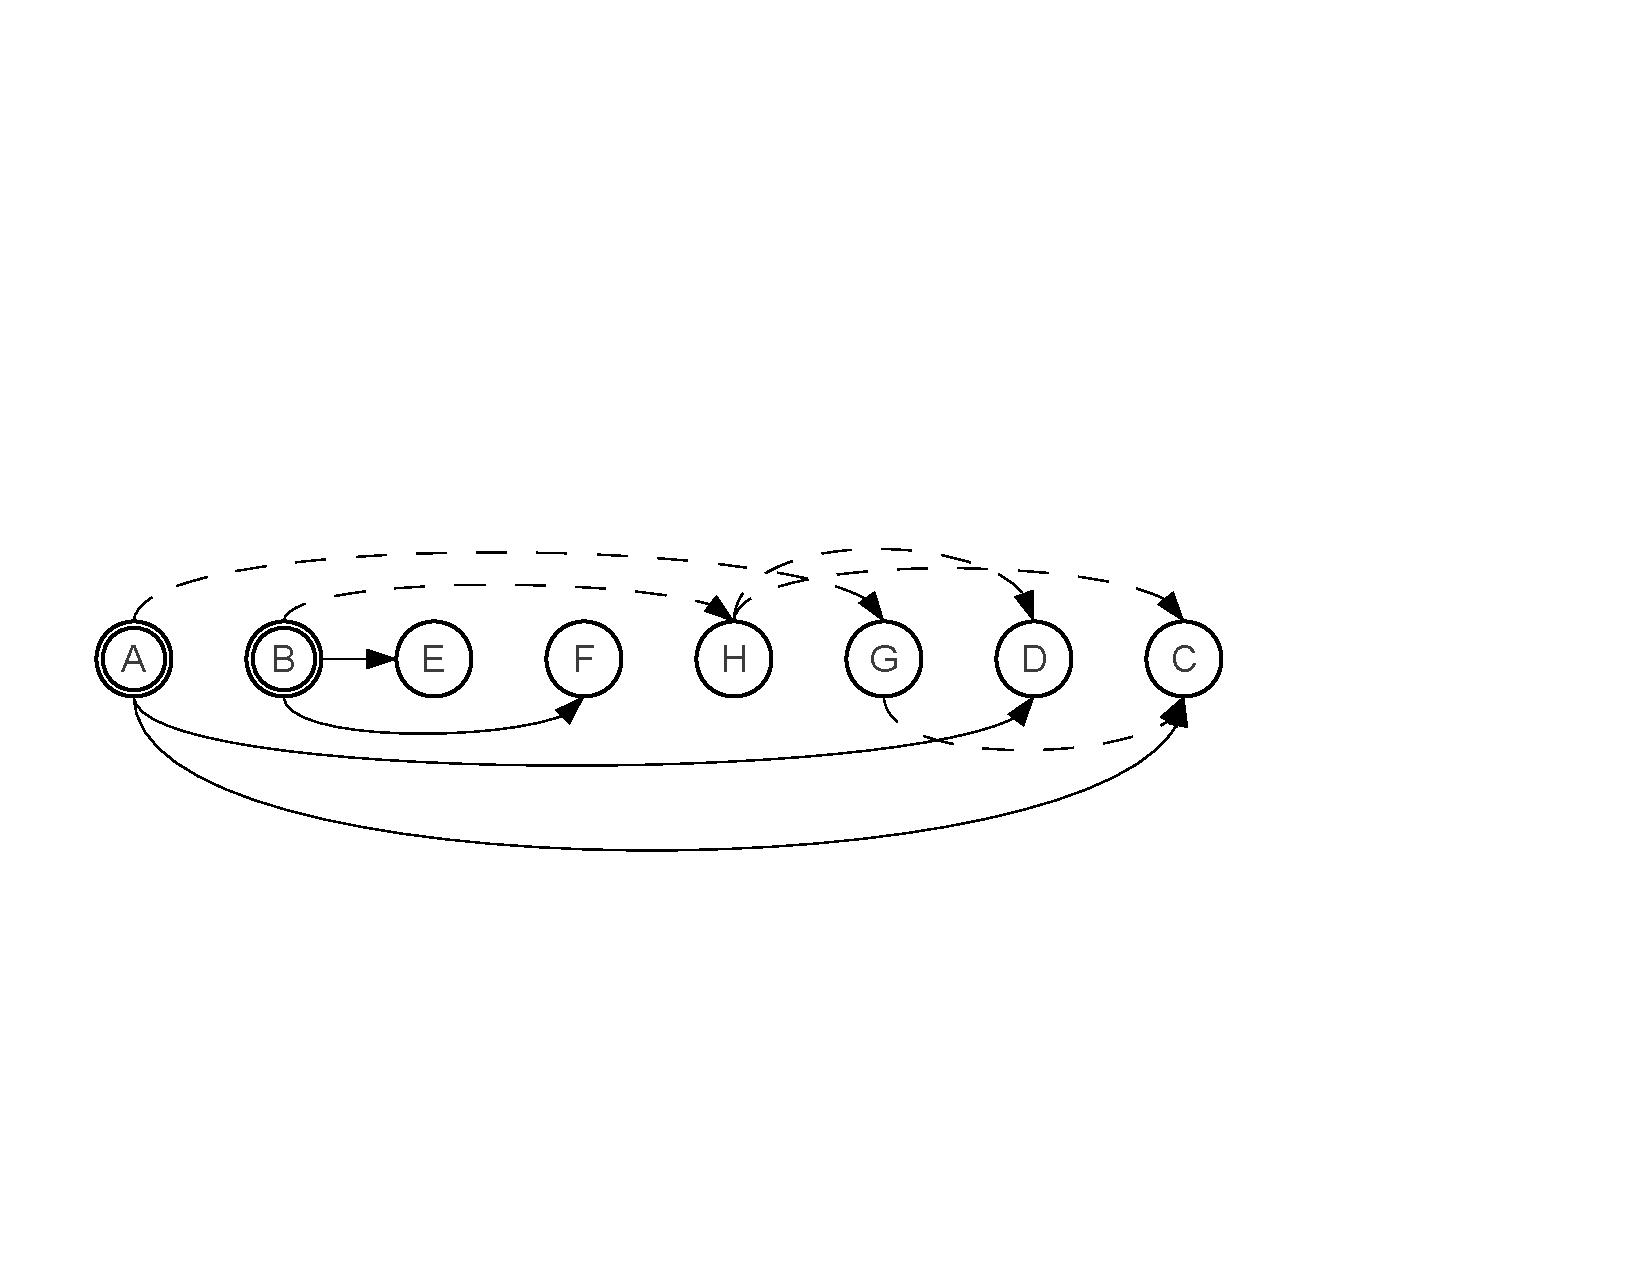
\includegraphics[scale=0.4]{figures/complementation/steps-0.pdf}
    \subcaption{Step 1}\label{hiercomp/fig:multiple:steps:0}
  \end{minipage}
  \begin{minipage}[b]{0.5\linewidth}
    \centering
    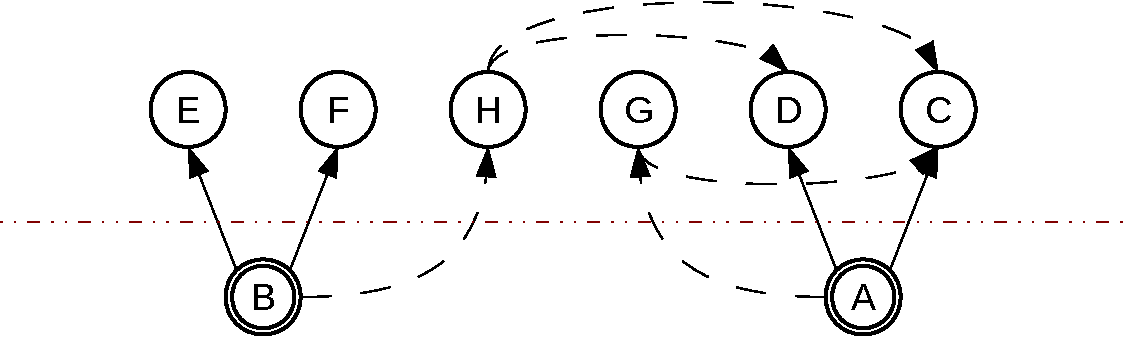
\includegraphics[scale=0.4]{figures/complementation/steps-1.pdf}
    \subcaption{Step 2}\label{hiercomp/fig:multiple:steps:1}
  \end{minipage}
  \vspace{0mm}                  % not sure why this adds space
  \\
  \begin{minipage}[b]{0.5\linewidth}
    \centering
    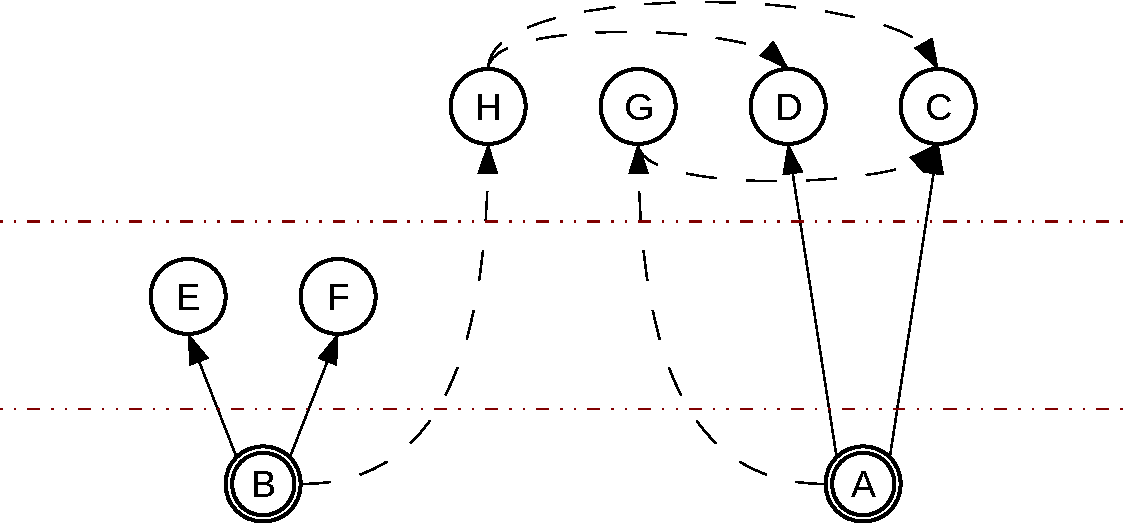
\includegraphics[scale=0.4]{figures/complementation/steps-2.pdf}
    \subcaption{Step 3}\label{hiercomp/fig:multiple:steps:2}
  \end{minipage}
  \begin{minipage}[b]{0.5\linewidth}
    \centering
    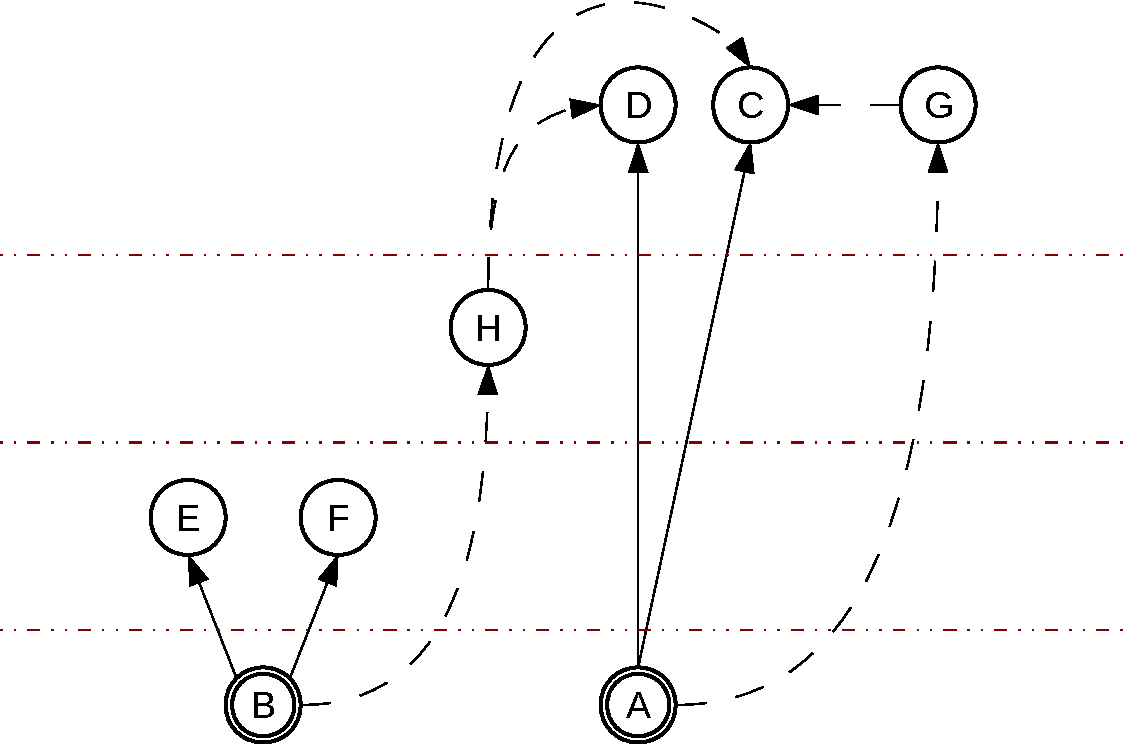
\includegraphics[scale=0.4]{figures/complementation/steps-3.pdf}
    \subcaption{Step 4}\label{hiercomp/fig:multiple:steps:3}
  \end{minipage}
  \vspace{0mm}
  \\
  \begin{minipage}[b]{0.5\linewidth}
    \centering
    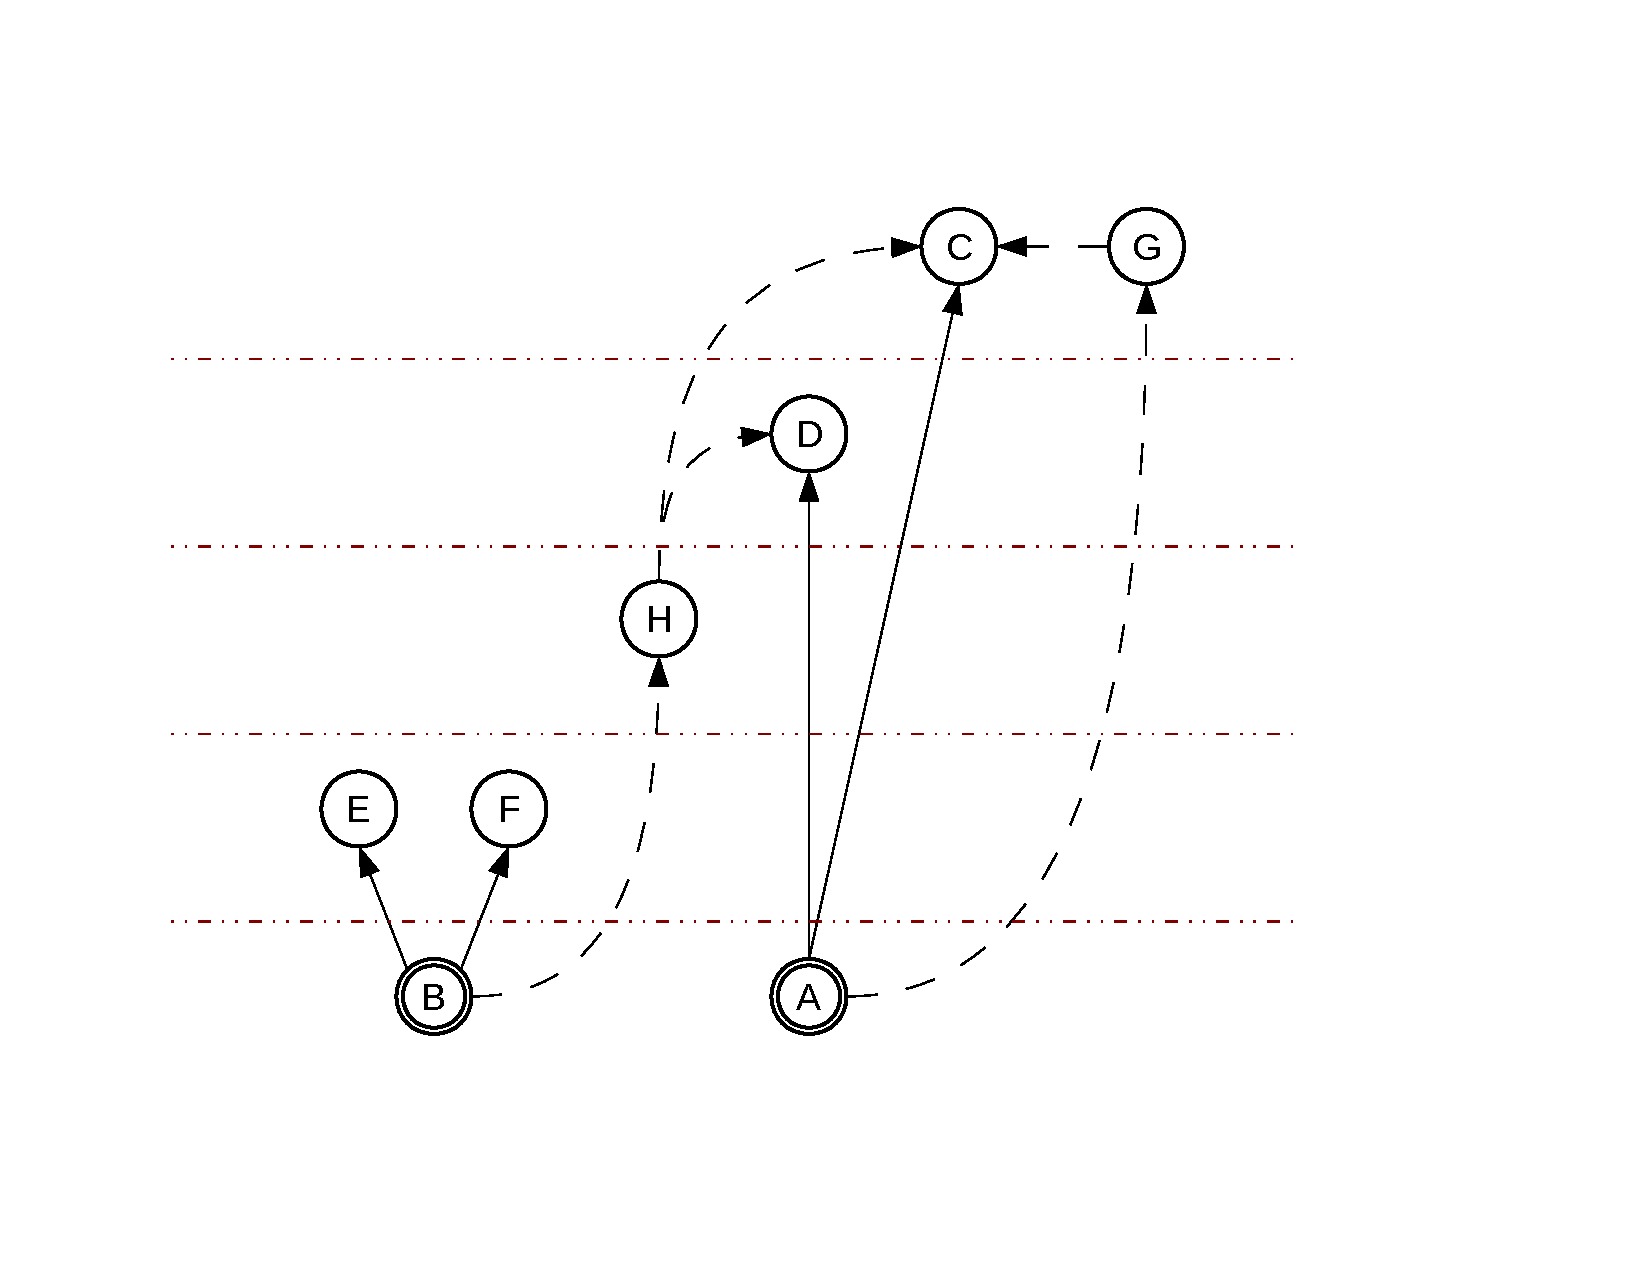
\includegraphics[scale=0.4]{figures/complementation/steps-4.pdf}
    \subcaption{Step 5}\label{hiercomp/fig:multiple:steps:4}
  \end{minipage}
  \begin{minipage}[b]{0.5\linewidth}
    \centering
    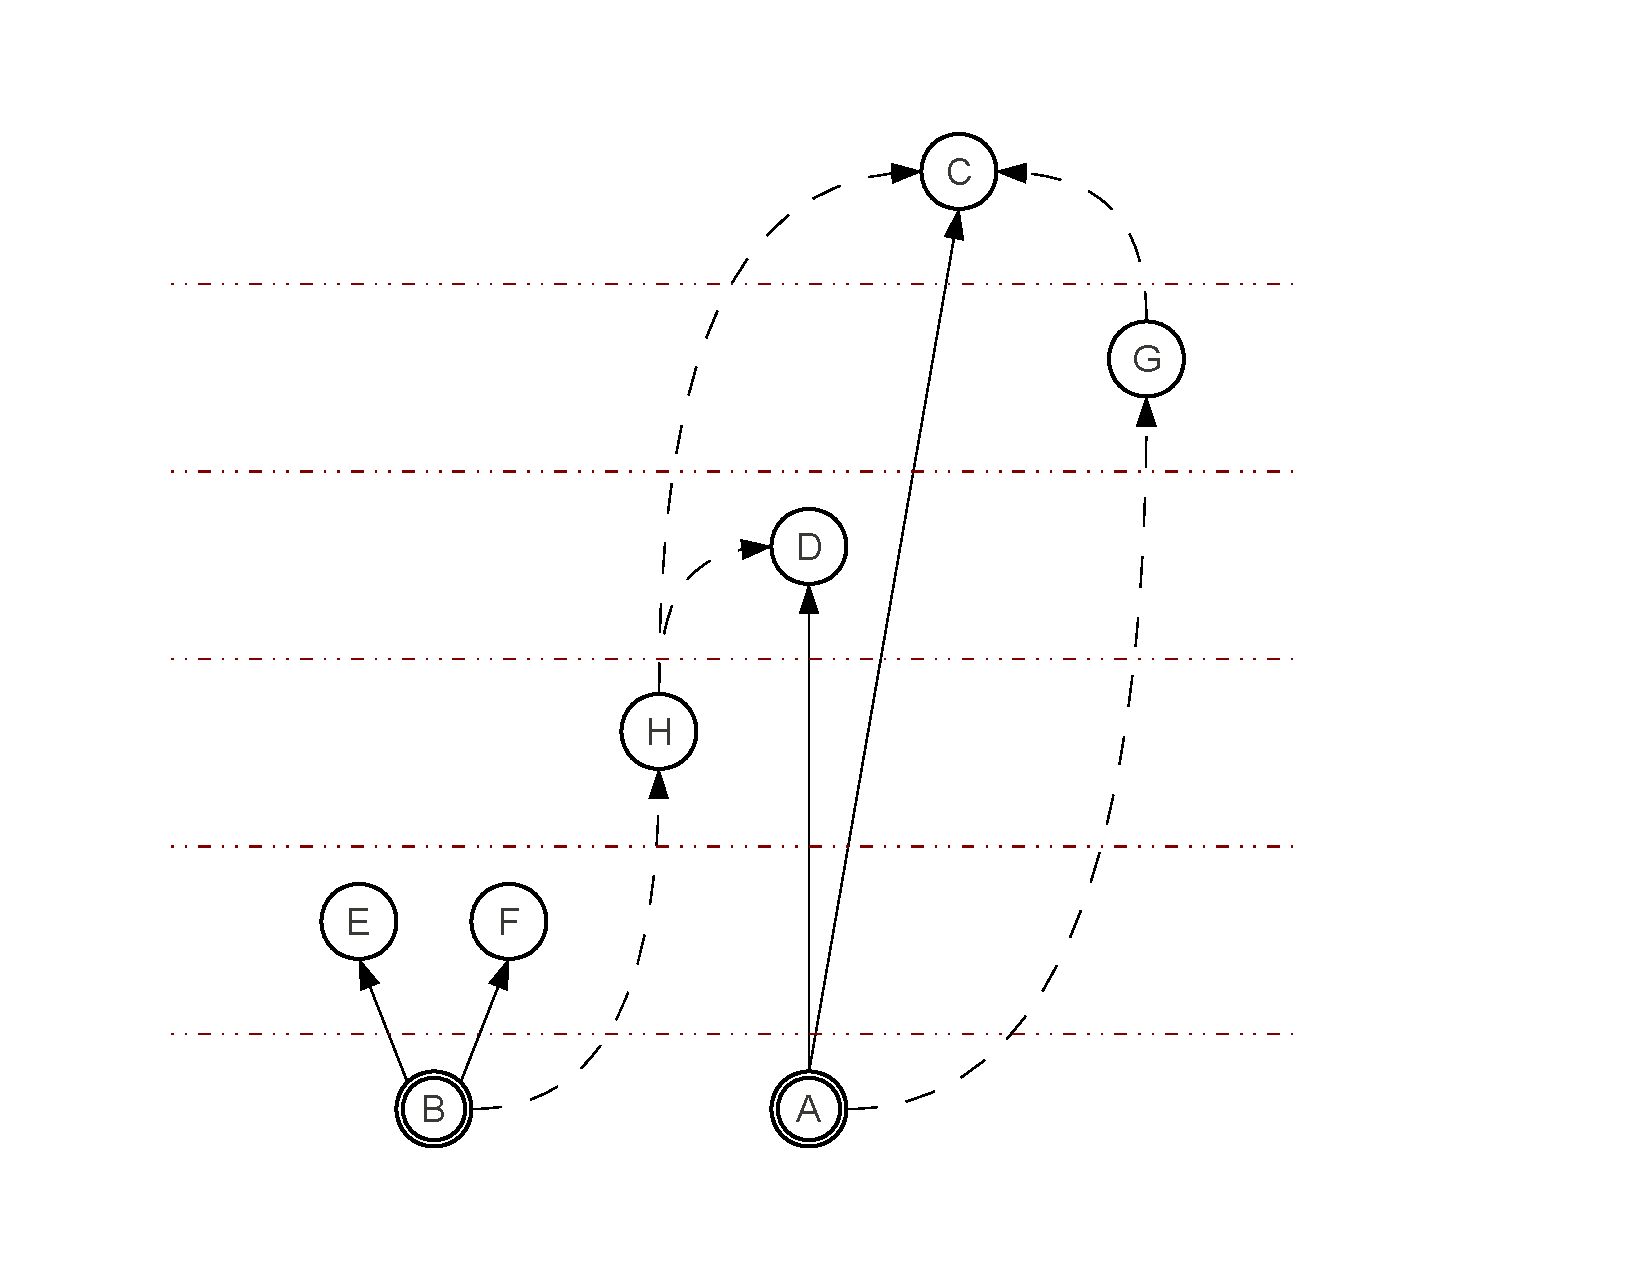
\includegraphics[scale=0.4]{figures/complementation/steps-5.pdf}
    \subcaption{Step 6}\label{hiercomp/fig:multiple:steps:5}
  \end{minipage}
  \caption[Stratification Example]{An example of the stratification
    produced by the multiple-inheritance solver for
    Example~\ref{hiercomp/fig:multipleHard}.}
  \label{hiercomp/fig:multiple:steps}
\end{figure*}

\begin{algorithm}
  \caption{Multiple-inheritance solver}
  \label{alg:multiple:strat}
  \small

  \hrulefill

  \begin{algorithmic}[1]
    \Function{solve}{$G = (V,E)$} \Let{$S$}{\Call{stratify}{$G$}}
    \Let{$U$}{$\{(s,t) \in E_{path} : s \in V_{known}\}$}
    \Let{$E_S$}{$E \setminus U$}
    \ForAll{$(s,t) \in U$}
       \State let $p \in \textit{proj}(s) : S[p] < S[t]$
       \Comment{such $p$ always exists}
       \Let{$E_S$}{$E_S \cup \{(p,t)\}$}
    \EndFor
    \State \Return $E_S$
    \EndFunction
    \algstore{alg:strat}
  \end{algorithmic}
%  \hrulefill
  \begin{algorithmic}[1]
    \algrestore{alg:strat}
    \Function{stratify}{$G = (V,E)$}
    \Let{$U$}{$\{(s,t) \in E_{path} : s \in V_{known}\}$}
    \ForAll{$t \in V$} \Let{$S_0[t]$}{$0$} \EndFor
    \For{$i = 0 \to |V|-1$} 
      \ForAll{$t \in V$}
        \Let{$S_{i+1}[t]$}{
          $\max
          \begin{Bmatrix}
            S_{i}[t] \\
            \maxof{(s,t) \in E}{\lbrace 1 + S_{i}[s] \rbrace} \\
            \maxof{ (s,t) \in U } {
            \lbrace
              1 + \minof{p \in \textit{proj}(s)}{\lbrace S_{i}[p] \rbrace} 
            \rbrace} \\ 
          \end{Bmatrix}$} \label{lst:line:formula} 
      \EndFor
      \If{$\forall v \in V : S_{i+1}[v] = S_{i}[v]$}
        \State \Return $S_{i}$  \label{lst:line:fixpoint} 
        \Comment{reached a fixpoint}
      \ElsIf{$\forall v \in V : S_{i+1}[v] = S_{i}[v] \Rightarrow S_{i}[v] = S_{i-1}[v]$}
        \State \algorithmicbreak \label{lst:line:unsat} 
        \Comment{no progress made on this step}
      \EndIf
%      \Let{$i$}{$i + 1$}
    \EndFor
    \State \Return error
    \Comment{unsolvable constraint graph}
    \EndFunction
  \end{algorithmic}

\end{algorithm}



Figure~\ref{hiercomp/fig:multiple:steps} presents an illustration of the
algorithm's application to the example of
Figure~\ref{hiercomp/fig:multipleHard}. The sets $\{C,D\}$ and $\{E,F\}$ are
the projection sets of nodes $A$ and $B$ respectively. At the first
step, all nodes will be placed in the lowest stratum. Note that, at
this point, all nodes could be placed in topological order:
Figure~\ref{hiercomp/fig:multiple:steps:0} is perfectly valid as the output
of a topological sort. However, this is not a
solution by our standards, since node $A$ cannot satisfy the edge to
$G$ because both of its projection nodes, $D$ and $C$, are placed
after $G$. Adding an edge from either one would be subject to creating
cycles. At the next step, our algorithm advances every node except $A$
and $B$, since all are edge targets. At step 3, things become more
interesting. Nodes $D,C$ have to be advanced by the same criterion,
since node $H$ contains edges to both, and they all reside in the same
stratum at step 2. However, nodes $H$ and $G$ have to be advanced for
a different reason, since they are targets of path-edges originating
from known nodes, namely $A$ and $B$, whose projections ($\{D,C\}$ and
$\{E,F\}$ respectively) were on the second stratum during the previous
step. At step 4, this condition ceases to exist for node $H$, since
nodes $E,F$ have ``stabilized'' at a lower stratum. This in turn
causes node $D$ to stabilize at step 5. At step 6, $G$ can also stay
put, since it is in a higher stratum than the lowest projection of
$A$, namely $D$. No nodes are advanced at step 7 (which is omitted in
Figure~\ref{hiercomp/fig:multiple:steps}), thus signifying that our
stratification has successfully converged to its final form. It is
therefore simple to compute a solution, by adding edges $(H,D),
(H,C), (G,C)$, $(D,G)$ and either $(F,H)$ or $(E,H)$
to the direct-edges $(A,C), (A,D), (B,E), (B,F)$. This set of edges
will constitute our final solution.

It is also easy to see that our algorithm would soundly detect that
the example of Figure~\ref{hiercomp/fig:unsat} is unsatisfiable. At the first
step, only known nodes $A,B$ would remain in the lowest stratum, but
on the next iteration all remaining nodes would advance again, thus
triggering the condition of failure (line~\ref{hiercomp/lst:line:unsat}), since
an iteration passed with no progress made.

% This projection set will serve as the domain for each path-edge that
% has not been satisfied yet. That is, in order to satisfy a path-edge
% $(s,t)$ we try to add a path-edge from a node in the projection set of
% $s$ to $t$. This may eventually lead to a cycle when all the edges in
% our constraint set have been transformed, in which case another
% candidate for the path-edge that was removed last from our constraint
% set is chosen. If none of the candidates for this path-edge succeeds,
% then our algorithm backtracks to a previous constraint and picks
% another node to satisfy it. If this process exhausts all combinations
% the search for a solution fails.
% %may end up trying all
% %possible combinations, which results in exponential time complexity in
% %the worst-case. In practice however, we will have to examine only a
% %small number of constraints, so this process will hardly be a
% %bottleneck.

A detailed proof of the correctness of our algorithm can be found in
Appendix~\ref{hiercomp/correctness}.


%-------------------------------------------------------------------------------
% Single Inheritance
%-------------------------------------------------------------------------------

\section{Hierarchy Complementation for Single Inheritance}
\label{hiercomp/single}

The problem for a single inheritance setting has a very similar
statement as in the earlier case of multiple inheritance, but markedly
different reasoning intricacies and solution approaches, due to a newly
arising constraint: every class in this setting can only have a
single parent.

Formally, our problem is modeled in much the same way as before. Our
input is again a directed graph $G = (V,E)$, with two disjoint sets of
nodes $V = V_{known} \disjunion V_{phantom}$ and two disjoint sets of edges
$E = E_{direct} \disjunion E_{path}$, where $E_{direct} \subseteq V_{known}
\times V$.  The difference is that the output of our algorithm should
be a directed \emph{tree} (instead of a DAG), $G_T = (V,E')$, such
that the same conditions as in the earlier case are satisfied:
\begin{enumerate}
\item
  \(\forall v_s \in V_{known}: (v_s,v_t) \in E' \Leftrightarrow (v_s,
  v_t) \in E_{direct}\)
\item \((v_s,v_t) \in E_{path} \Rightarrow\) there is a path from
  \(v_s\) to \(v_t\) in \(G_T\)
\end{enumerate}

Without loss of generality, we assume that there exists a ``root''
node $n_r \in V_{known}$ that is a common supertype for all of our
types. If no such type exists, we can create an artificial one, by
adding extra constraint edges. In this way, we can be certain that
computing a graph with a single outgoing edge for all nodes (but one)
will form a tree instead of a forest.

% Thus, each type may now have multiple supertypes. The only limiting
% constraint is  that we cannot have cycles in the resulting
% hierarchy. This constraint also applied to the single inheritance case, where
% the algorithm would detect such a cycle, if no unconstrained nodes
% were left in a non-empty graph (Algorithm\ref{hiercomp/alg:single:simple},
% function \textsc{placeUnder()}---line~\ref{hiercomp/lst:line:cycle}).

% Based on theses examples we see that solving the problem seems to
% require a search.\footnote{We have thus far failed to either cast the
% problem as a (polynomial) stratification or flow problem, or to prove
% NP-completeness, despite significant efforts. Nevertheless, this is
% unlikely to affect the practical algorithm used for the solution in
% JPhantom: our current approach is simple and very fast in practice.}
% Therefore our algorithm for the multiple inheritance case is a
% straightforward backtracking exhaustive search for the satisfaction of
% all constraints of the form of Figure~\ref{hiercomp/fig:choice}.


The problem is quite hard in its general setting. There are several
patterns that necessitate a complex search in the space of
possibilities. Figures~\ref{hiercomp/fig:single1}-\ref{hiercomp/fig:single4} show some
basic patterns that induce complex constraints. All nodes reachable
from a single one need to be linearly ordered
(Figure~\ref{hiercomp/fig:single1} shows the simplest case). This requires
computing an ordering (i.e., guessing a permutation) of these
nodes. Other constraints can render some of the permutations
invalid. The basic pattern behind such restrictions is that of
Figure~\ref{hiercomp/fig:single2}: there are hierarchies that cannot be
related. Combining the two patterns suggests that there needs to be a
search in the space of permutations for a valid one:
Figures~\ref{hiercomp/fig:single3} and \ref{hiercomp/fig:single4} show some simple
cases.

% CHECK subcaption alignment everywhere!!

\begin{figure*}[htb]
  \vspace{-5mm}
  \begin{minipage}[t]{0.5\linewidth}
    \centering
    \includegraphics[scale=0.6]{figures/complementation/sing-inh-pat1.pdf}
    \subcaption{B and C must be subtype-related (in either
      direction).}\label{hiercomp/fig:single1}
  \end{minipage}
  \hspace{0.4in}
  \begin{minipage}[t]{0.5\linewidth}
    \centering
    \includegraphics[scale=0.6]{figures/complementation/sing-inh-pat2.pdf}
    \subcaption{D and E cannot be subtype-related.}\label{hiercomp/fig:single2}
  \end{minipage}
  \\
  \begin{minipage}[t]{0.5\linewidth}
    \centering
    \includegraphics[scale=0.6]{figures/complementation/sing-inh-pat3.pdf}
    \subcaption{A has to be a subtype of F.}\label{hiercomp/fig:single3}
  \end{minipage}
  \hspace{0.2in}
  \begin{minipage}[t]{0.5\linewidth}
    \centering
    \includegraphics[scale=0.6]{figures/complementation/sing-inh-pat4.pdf}
    \subcaption{A has to be a subtype of either G or
      H.}\label{hiercomp/fig:single4}
  \end{minipage}
  \caption{Single Inheritance Basic Patterns}
\end{figure*}

Composing such constraints into more complex hierarchies gives an idea
of the difficulty of the search involved. Figure~\ref{hiercomp/fig:hard:or}
shows an example where it is hard to see without complex
reasoning which of the $E$, $F$, $G$ nodes have to be placed
above $A$ and which cannot.

\begin{figure}
  \centering
  \includegraphics[scale=0.7]{figures/complementation/sing-inh-or.pdf}
  \caption[Harder composite example of single-inheritance
  constraints]{ Harder composite example of single-inheritance
    constraints.  The (undirected) path from $B$ to $C$ through
    $E,F,G$ implies that $(A <: E) \lor (A <: F) \lor (A <:
    G)$. However, since $F$ is the first common known supertype of $M$
    and $N$, and $A$ just a supertype of both, $F <: A$, and thus
    $(A <: E) \lor (A <: G)$. }
\label{hiercomp/fig:hard:or}
\end{figure}

%%You keep using that word, comprise. I don't think it means what you
%%think it means.

Clearly the problem can be modeled as a constraint satisfaction
problem instance, where $V_{phantom}$ is our set of variables and $V$
is the domain of values (representing the variable's direct
supertype). The path-edges and the absence of cycles constitute our
constraints. This requires an exponential search in the worst
case. Indeed, our implementation performs precisely such an exhaustive
search, but with a heuristic choice of nodes so that the search tries
to satisfy the constraints introduced by the patterns in
Figures~\ref{hiercomp/fig:single1} and
\ref{hiercomp/fig:single2}---i.e., the pattern of
Figure~\ref{hiercomp/fig:single1} is identified, all induced
permutations are tried, and the pattern of
Figure~\ref{hiercomp/fig:single2} is used to prune them eagerly,
instead of waiting to detect failure later.

Most importantly, our approach provides special handling for a
simple but practically quite common case. In this special case,
there is a polynomial algorithm for solving the problem and exhaustive
search is avoided.
%\footnote{More accurately, the special case algorithm
%is used as a subroutine and exhaustive search is performed by having
%the special case algorithm return different solutions when one fails.}

\begin{algorithm}[thp]
  \caption{Single-inheritance solver for strictly known direct-supertypes}
  \label{hiercomp/alg:single:kdirect}
  \small
  \hrulefill

  \begin{algorithmic}[1]
    \Function{solve}{$G = (V,E)$}
    \State{let $R$ be the ``\emph{root}'' node of $V$}
    \State{let $S$ be the tree of known nodes $(V_{known}, E_{direct})$}
    \ForAll{$(s,t) \in E_{path} : s \in V_{known}$}
      \If{$\nexists$ path $s \leadsto{} t$ in $S$}
        \State \Return error (unsatisfiable constraint)
      \EndIf
      \Let{$E_{path}$}{$E_{path} \setminus \{(s,t)\}$}
      \Comment{remove already satisfied edge}
    \EndFor
    \ForAll{$v \in V_{phantom}$}
      \State\Call{makeSet}{$v$}
      \Comment{create single-element disjoint sets}
    \EndFor
    \ForAll{$(s,t) \in E_{path} : t \in V_{phantom}$}
      \State\Call{union}{$s$, $t$}
      \Comment{merge two connected (phantom) components}
    \EndFor
    \Comment{result: undirected connected components (UCCs)}
    \ForAll{$v \in V_{phantom}$}
      \Let{$k$}{\Call{find}{$v$}}
      \Let{$\textit{top}[k]$}{$R$}
      \Comment{initially ``root''}
    \EndFor \Comment{init UCC's lowest common known superclass (LCS)}
    \ForAll{$(s,t) \in E_{path} : t \in V_{known}$} \Comment{must be $s \in V_{phantom}$}
      \Let{$k$}{\Call{find}{$s$}}
      \If{$\exists$ path $t \leadsto \textit{top}[k]$ in $S$}
        \Let{$\textit{top}[k]$}{$t$}
        \Comment{lower superclass found, update LCS}
      \ElsIf{$\nexists$ path $\textit{top}[k] \leadsto t$ in $S$}\label{hiercomp/lst:line:crossover}
        \State \Return error (unsatisfiable constraint)
      \EndIf
    \EndFor
    \ForAll{$k \mapsto v$ in \textit{top}}
    \Comment{for each UCC and its LCS}
      \Let{$U$}{$\{(s,t) \in E_{path} : t \in V_{phantom} \land \textsc{find}(s) = k\}$}

      \Comment{directed subgraph of original over nodes of this UCC}
      \Let{$L$}{a topological order of $U$}
      \Comment{linearize subgraph}
      %% \ForAll{$(x,y)$ in $zip(L,tail(L))$}
      %% \EndFor
      \Let{$hd$}{the top node of $L$}
      \Let{$S$}{$S \cup L \cup \{(hd,v)\}$} 
%      \While{$L$ is not empty}
%        \State $hd::L' = L$
%        \Comment{unpack head-tail of list $L$}
%        \Let{$S[hd]$}{$v$}
%        \Comment{set $v$ as the direct-supertype of $hd$ }
%        %% \Comment{set $v$ as the direct-supertype of $hd$}
%        %% \State add $(v,hd)$ to $S$
%        \Let{$v, L$}{$hd, L'$}
%        \Comment{advance $L$ and renew $v$}
%      \EndWhile
    \EndFor
    \State \Return{$S$}
    \EndFunction
  \end{algorithmic}
\end{algorithm} 



%%% Local Variables: 
%%% mode: latex
%%% TeX-master: "../../doc"
%%% End: 


\paragraph{Simplified setting: No direct-edges to phantom nodes.}

It is easy to solve the problem in the case that there are no direct
edges from known nodes to phantom nodes. Since we are in a
single-inheritance setting, this means that no class in the known part
of the program has a superclass in the complement that we are trying
to produce. In this case, we have that $E_{direct} \subseteq
V_{known}\times V_{known}$. The extra condition allows us to employ a
fast polynomial time algorithm. This interesting case of our problem
is very common in practice. Intuitively, the ease of dealing with this
case stems from avoiding the search in the space of permutations when
the input contains patterns such as those in Figure~\ref{hiercomp/fig:single3}:
if two permutations have elements in common (e.g., the permutation of
$B$ and $F$, and that of $F$ and $C$ in Figure~\ref{hiercomp/fig:single3}) they
cannot include nodes that are guaranteed to be subtype-unrelated (such
as $B$ and $C$ in this example) and all unknown nodes have to be below
the known ones in any solution.

Algorithm~\ref{hiercomp/alg:single:kdirect} first removes path-edges
originating from known-nodes, after verifying that the corresponding
paths indeed exist. It then uses union/find data structures to compute
connected components of phantom nodes, while treating path-edges
as \emph{undirected} edges: anything connected through such edges can
safely end up in a single linear ordering. Then, for each phantom
undirected connected component, it computes the lowest known-node to
serve as the first-common-supertype of all of this component's phantom
nodes. Note that when two known-nodes are reachable by two phantom
nodes of the same connected component (in the phantom subgraph), then
one of them ought to be a supertype of the other, or else no solution
can exist in a single inheritance setting. This condition is captured
in line~\ref{hiercomp/lst:line:crossover}. After the first common (known)
supertype for every connected component has been computed, a mere
topological sort, i.e. placing all relevant nodes in a total order, is
enough to satisfy all of this component's constraints. This may
introduce many superfluous edges in the solution: these edges are not
actually required by our constraints (since a topological order is a
total order). In practice, we produce a partial order by using a
variant of topological sort that generates a tree instead of a list as
its result, but a full topological sort also satisfies the correctness
requirements of the algorithm. (We return to the topic of why we
actually want a weaker ordering in Section~\ref{hiercomp/java}.)

In the example of Figure~\ref{hiercomp/fig:kdirect:ex},
Algorithm~\ref{hiercomp/alg:single:kdirect} first checks and removes the
$(F,A)$ path-edge. Then the phantom nodes are divided in the following
phantom connected components: $\{G,H,I\}$, $\{J,K,L\}$, and
$\{M\}$. The first common known supertype for each component is $B$,
$F$, and $F$ respectively. Each component is then linearized, which
generates the following complete orders that are appended to the
output: $I <: H <: G <: B$, $K <: J <: L <: F$, and $M <: F$.

% CHECK list of figure names

\begin{figure}[t]
  % \hspace{-6mm}
  \begin{minipage}[b]{.5\linewidth}
    \centering
    \includegraphics[scale=0.6]{figures/complementation/sing-inh-direct.pdf}
    \subcaption{Constraint Graph}\label{hiercomp/fig:stree1:simple}
  \end{minipage}
  % \hspace{-5mm}
  \begin{minipage}[b]{.5\linewidth}
    \centering
    \includegraphics[scale=0.6]{figures/complementation/sing-inh-direct-solution.pdf}
    \subcaption{Solution}\label{hiercomp/fig:cgraph1:simple}
  \end{minipage}
  \caption[Single Inheritance Algorithm Example]{%
    Algorithm~\ref{hiercomp/alg:single:kdirect} - Example. }
  \label{hiercomp/fig:kdirect:ex}
\end{figure}

%% Do we care? Seems like a leftover.
%A phantom-only input, i.e. $V = V_{phantom}$, $E = E_{path}$, poses no
%difficulties in this setting too, since a single topological sort
%would suffice as an acceptable solution. (A solution, for our
%purposes, yields a correct program complement exactly when one exists,
%i.e., is both sound and complete.)



\begin{comment}
%%%%%%%%%%%%%%%%%%% Old stuff follow

However, in order to achieve a solution that generalizes well to
harder cases, we would like to avoid ordering nodes if there is no
need for them to be ordered. The result will be a tree and not a
linear order (in the general case). Specifically, we would like to
compute a partial order relation,\footnote{Throughout this chapter, our
use of the term ``partial order'' denotes an irreflexive partial
order.} $\ll$, such that:

\begin{itemize}
\item $\ll$ subsumes the input constraints, i.e., $v_a \ll v_b$ if $(v_a,v_b) \in E$
\item if $v_c \ll v_a$ and $v_c \ll v_b$ then either $v_a \ll v_b$ or $v_b \ll v_a$
\item $\ll$ is transitively closed
\item $\ll$ is minimal, i.e., removing any pair from the relation would violate
the above rules.
\end{itemize}

The addition of the second rule, above, is a hallmark feature of the
hierarchy complementation problem. Consider the input of
Figure~\ref{hiercomp/fig:diamond}. The $(B,A)$ and $(C,A)$ edges guarantee that
both $B$ and $C$ will be ordered below $A$ in the result.  However, we
also know that they should be ordered relative to each other: the
$(D,B)$ and $(D,C)$ edges enforce this requirement, since there can
only be a single path from $D$ to the root of the hierarchy and both
$B$ and $C$ must be on it. Note that, in the absence of
other ordering constraints, we could have either $B \ll C$ or
$C \ll B$---both options would yield $\ll$ relations that satisfy the
above requirements, for this example.

%% \begin{defn}
%%   A solution $G_S = (V,E')$ to a set of subtype constraints $G_C =
%%   (V,E)$ is minimum if and only if, $\forall x,y \in V$ such that a
%%   path $p = x \ldots y$ exists in $G_S \Rightarrow$ .
%% \end{defn}

\begin{figure}
  \centering \includegraphics[width=0.2\textwidth]{figures/complementation/diamond.pdf}

  \caption{In any solution of these subtyping constraints, B and C
  have to be below A, but also they have to be relatively ordered with
  each other, since D must find both on its (single inheritance) path
  to the root.}
\label{hiercomp/fig:diamond}
\end{figure}

Algorithm~\ref{hiercomp/alg:single:simple} produces an ordering relation
(represented as a ``solution'' set of ``direct parent'' edges, $S$)
whose transitive closure satisfies the requirements for
$\ll$,\footnote{I.e., the algorithm computes the \emph{transitive
reduction} of $\ll$, or, in diagram form, the Hasse diagram of the
$\ll$ partial order, i.e., the depiction of the partial order with
direct-predecessor-only edges.} or signals an error if none
exists. The algorithm is given in pseudocode, mixed with informal
well-understood operations when their precise description would be
tedious. Such concepts include ``remove vertex and all incoming
edges'', ``undirected view of a directed graph'', ``maximally
connected component'', ``restriction of a graph to a subset of its
nodes''.

Function \textsc{placeUnder()} augments the solution being generated
by placing every node of its first argument, graph $G$, under its
second argument, node $n$. The invariant maintained across recursive
invocations is that, on entry, $n$ is a node of $G$ with no outgoing
edges and all nodes of $G$ can reach $n$ \emph{when the edges of G are
converted to undirected edges}.  The key to the algorithm is precisely
this property: we order below a node all other nodes that can reach it
with edges considered in any direction, thus satisfying the properties
of the $\ll$ definition. A key lemma (proven by induction) is that if
an unconstrained node (i.e., one without outgoing edges), $u$, can
reach another node, $k$, via any combination of up-or-down subtyping
inferences, then $u$ and $k$ have a common descendant, i.e., a node
that has (directed) paths to both. Therefore $u$ and $k$ must be
relatively ordered (although it is not known in which direction).  By
also picking to place a subtree under one of its nodes with no
outgoing edges (mimicking a plain topological sort), we ensure that
the arbitrary ordering picked (to satisfy the second rule of the $\ll$
definition) does not violate explicit ordering constraints in the
input (per the first rule of the $\ll$ definition). The above
properties also serve as a proof sketch for the correctness of
Algorithm~\ref{hiercomp/alg:single:simple} relative to the definition of $\ll$.

% Thus, to create our solution, given that our
%constraint graph is weakly connected---and if it's not, we can make it
%so by adding auxiliary edges to the \emph{root} node---we only have to
%call \textsc{placeUnder()} with the \emph{root} node as its second
%argument.

\begin{algorithm} 
  \caption{Single-inheritance phantom-only solver}
  \label{alg:single:simple}
  \hrulefill

  \begin{algorithmic}[1]
    \Function{solve}{$G = (V,E)$}
    \State{let $v_r$ be the ``\emph{root}'' node of $V$}
    \State \Return \Call{placeUnder}{$G$, $v_r$}
    \EndFunction
  \end{algorithmic}

  \hrulefill

  \begin{algorithmic}[1]
    \Function{placeUnder}{$G = (V,E)$, $n$}
       %% \Comment $G_u$ reflects changes in $G$
       \Let{$S$}{$\emptyset$}
       \State remove vertex $n$ (and its incoming edges) from $G$ 
       \Let{$V_n$}{$\left\{ x \in V : \not \exists (x,y) \in E \right\}$} \Comment all nodes with no outgoing edges
       %% \Comment unconstrained nodes
       %% \State $UV \gets V \setminus \left\{ x : (x,y) \in E
       %% \right\}$
       \While{$V_n \neq \emptyset$} 
          \State $x \gets$ \Call{pick}{$V_n$, $n$}
          \State $V_n \gets V_n \setminus \left\{x\right\}$ 
          \If{$x \in V$} \Comment otherwise it has been ordered by earlier iteration
             \Let{$S$}{$S \cup \{(x,n)\}$} \Comment add edge $(x,n)$ to solution
             %% \Comment $x$ extends $n$
             \State let $G_u$ be the undirected view of $G$ 
             \State let $V'$ be the nodes of the maximally connected 
               component of $G_u$ that contains $x$
             \State let $G' = (V',E')$ be the restriction of $G$ to $V'$ \Comment Note: $G'$ is directed
             \State $G \gets (V \setminus V', E \setminus E')$ \Comment remove from $G$ all nodes in $V'$ and adjacent edges
%             \ForAll{$v \in V'$}
%             \State remove $v$ and its adjacent edges from $G$
%             \EndFor
%             \Let{$S_x$}{\Call{placeUnder}{$G' = (V',E')$, $x$}} \Comment recurse for the removed subgraph
             \Let{$S$}{$S \cup $ \Call{placeUnder}{$G' = (V',E')$, $x$}} \\
                               \Comment recurse for removed subgraph, accumulate solution edges
          \EndIf
       \EndWhile
       \If{$G$ has edges} \Comment all nodes have outgoing edge (cycle)
         \State error: no solution  \label{lst:line:cycle}  %(graph has at least one cycle)
       \EndIf
       \State \Return $S$
    \EndFunction
  \end{algorithmic}

  \hrulefill

  \begin{algorithmic}[1]
    \Function{pick}{$V$, $n$}
    \State \Return random element of $V$
    \EndFunction
  \end{algorithmic}
\end{algorithm} 



An example is given in Figure~\ref{hiercomp/fig:ex1:simple}. We assume that
node $A$ is the \emph{root} node. Therefore, the algorithm will first
call \textsc{placeUnder($G_C$, $A$)} and then erase the edges
$\{(B,A), (C,A), (D,A), (E,A), (I,A)\}$. The set of unconstrained
nodes, $V_n$, will contain the nodes $B,C,E$. Without loss of
generality, we assume that the \textsc{pick()} function always returns
the lexicographically smaller node of its candidates. Thus, the edge
$(B,A)$ is added to the solution, and \textsc{placeUnder()} is
recursively called for the component of $G$ that contains only the
edge $(D,B)$, which is then also removed from $G$ and added to the
solution. The control flow will go back to node $A$, pick the next
unconstrained node, $C$, and call \textsc{placeUnder()} again after
adding the edge $(C,A)$ to the solution. This time, the component
computed (by undirected reachability) to be under $C$ will contain
every remaining node, and will therefore prevent any other node from
being placed directly under $A$. After edge $(F,C)$ is removed, the
unconstrained nodes now become $E$ and $F$. The edge $(E,C)$ is added
and $(G,E),(H,E)$ are removed. Again, every remaining node will be
placed under $E$. The node $F$ is picked among $F,G,H$, edge $(F,E)$
is added, and $G'$ gets every remaining edge except $(H,E)$ because
$H$ is (undirected-)unreachable by $F$. Edge $(H,E)$ will be added
eventually, after $G,J,I$ have been recursively placed under $F$ in
this order.

\begin{figure}
  \centering
  \subfloat[Constraint Graph]{
    \includegraphics[scale=0.4]{images/cgraph1.pdf}
    \label{hiercomp/fig:stree1:simple}
  }
  \subfloat[Solution]{
    \includegraphics[scale=0.4]{images/stree1.pdf}
    \label{hiercomp/fig:cgraph1:simple}
  }
  \caption{%
    Algorithm~\ref{hiercomp/alg:single:simple} - Example
  }
\label{hiercomp/fig:ex1:simple}
\end{figure}



%
%We can then decouple the two different types of edges into the $f_i$
%mapping and a graph $G_C = (V,E_{path})$. For ease of notation, we
%will use $f_i$ and $G_C = (V,E)$ from now on, as a shorthand, but each
%edge of $G_C$ will represent a path-edge: $\forall (x_1,x_n) \in
%E : \text{there exists a path } (x_1,x_2,\ldots, x_n) \text{ in } G_T$.
%
%
%Let us ignore, for now, the subset of fixed edges that corresponds to
%$f_i$ and should eventually be present in any solution. This variation
%of our problem means that we allow only phantom types in our
%constraints, for which no supertype information exists, whatsoever. A
%simple solution to this problem would be a topological order
%w.r.t. our constraints $E$.


\paragraph{Full single inheritance setting: known and phantom nodes.}

We can extend our algorithm to support an existing class hierarchy by
combining a simple preprocessing step and a biasing of
function \textsc{pick} so that it preferentially returns a direct
child, if one exists in the input. Recall that our input is now two
distinguished sets of nodes, $V_{known}$, $V_{phantom}$ and similarly
for edges, $E_{direct}$, $E_{path}$.  For notational convenience we
represent $E_{direct}$ as a function $f_i:V_{known} \rightarrow
V$. (Since we are in a single inheritance setting, we can guarantee
that $E_{direct}$ is a function from its first argument: if a node
$v \in V_{known}$ has more than one outgoing edge then the problem is
immediately unsolvable. Our solution edge set is similarly a function,
since we are computing a tree.)


%Similarly, since $G_T$ has to be a tree, we can also encode our
%solution (output) as another mapping, $f_o:V \rightarrow V$.  Both of
%these mappings map a type (key) to its \emph{direct}-supertype
%(value). Thus, the first constraint of our solution becomes: $\forall
%v \in V_{known} : f_o[v] = f_i[v]$, where $f_i[v]$ denotes the known
%direct supertype of $v$ (given as input), and $f_i$ can now be viewed
%as a partial solution that should be preserved by our final solution
%$f_o$.

The preprocessing step consists of merely adding subtyping edges from
all known supertypes of a type to all its unknown ones. In other
words, the principle is that if a node $n$ can reach another node $m$
through a path of $E_{direct}$ edges, while $n$ reaches $m'$ via an
$E_{path}$ edge, then the solution should have a path from $m$ to
$m'$.  By transitively following the $f_i$ function (i.e.,
$E_{direct}$ edges) we can add outgoing edges to all nodes found on
this path, so they will never be placed above a node ordered relative
to their descendant via $E_{path}$, thus violating the requirement of
preserving the input hierarchy. This is shown in
Algorithm~\ref{hiercomp/alg:single:ext}. Function \textsc{solve()} performs
the preprocessing step while keeping the core logic, i.e. the earlier
\textsc{placeUnder()} function, intact. Function \textsc{pick()}
prioritizes known direct descendants, in order to maintain the
$E_{direct}$ edges in the output.

\begin{algorithm} 
  \caption{Single-inheritance extended solver}
  \label{hiercomp/alg:single:ext}

  \hrulefill

  \begin{algorithmic}[1]
    \Function{solve}{$G = (V,E)$}
     where $V = V_{known} \cup V_{phantom}$ and $E = E_{direct} \cup E_{path}$
    \State \Global $f_i$ \Comment global var as convenience, to keep same args for \textsc{placeUnder}, \textsc{pick}
    \ForAll{$(v_s,v_t) \in E_{direct}$}
      \If{$\exists (v_s, v_{t'}) \in E_{direct}$ such that $v_t \neq v_{t'}$}
        \State error: input not a tree
      \Else
        \Let{$f_i[v_s]$}{$v_t$}
      \EndIf
    \EndFor
%    \ForAll{$c \in V_{known}$}
      %% \State add edge $(c,f_i[c])$ to $E$ \label{hiercomp/lst:line:direct}
      \ForAll{$(c,c_s) \in E_{path}$}
        \While{$f_i[c] = p$} \Comment while there exists a known parent, which we shall call $p$
          \If{$p \neq c_s$}  \Comment just for tolerating extraneous path edges in input
            \State $E \gets E \cup
            \left\{(p,c_s)\right\}$ \label{hiercomp/lst:line:add}
            \Comment no need to update $E_{path}$, \textsc{placeUnder} only uses $E$
% $E$ add edge $(p,c_s)$ to $E$ \label{hiercomp/lst:line:indirect}
          \EndIf
          \Let{$c$}{$p$}
%          \Let{$c$}{$f_i[c]$}
        \EndWhile
      \EndFor
%    \EndFor
    \State{let $v_r$ be the ``\emph{root}'' node of $G$}
    \State \Return \Call{placeUnder}{$G$, $v_r$} \Comment{\textsc{placeUnder} treats direct and path edges the same}
    \EndFunction
  \end{algorithmic}

  \hrulefill

  \begin{algorithmic}[1]
    \Function{pick}{$V$, $n$}
    \If{$\exists v \in V: f_i[v] = m$} \label{hiercomp/lst:line:priority}
      \If{$n \neq m$}
        \State error: crossover %% \label{hiercomp/lst:line:crossover}
      \Else
        \State \Return $v$
      \EndIf
    \Else
    \State \Return random element of $V$
    \EndIf
    \EndFunction
  \end{algorithmic}
\end{algorithm} 



For example, in Figure~\ref{hiercomp/fig:ex1:ext} we can see how the solution
of Figure~\ref{hiercomp/fig:ex1:simple} is altered if we take a given class
hierarchy into account. Let $V_{known} = \{F,J\}$ and $E_{direct}
= \{(F,C),(J,F)\}$. The solid edges denote the constraints added due
to $f_i$, while the newly added edges $(F,G),(C,G)$ have been inserted
because of $(J,G)$. Since $G$ is surely a supertype of $J$ and we know
that $F$ is the direct supertype, we can soundly add the edge $(F,G)$
to preserve their respective order. After $(F,G)$ has been added, and
because $f_i[F] = C$, we can soundly add $(C,G)$ and then reach a
fixpoint.

% (line~\ref{hiercomp/lst:line:indirect}).

Line~\ref{hiercomp/lst:line:priority} in the \textsc{pick()} function will
choose a \emph{direct} subtype according to $f_i$, over any other
unconstrained node. For instance, if ``$f_i[C] = A$'' were part of the
input in the earlier pattern of Figure~\ref{hiercomp/fig:diamond}, then
the \textsc{pick()} function would choose node $C$ among $V = \{B,C\}$
to place next, resulting in the $A \leftarrow C \leftarrow
B \leftarrow D$ ordering (and not $A \leftarrow B \leftarrow
C \leftarrow D$, as produced by settling arbitrary node choices according
to lexicographic order).

In line \ref{hiercomp/lst:line:crossover} of the \textsc{pick()} function, an
error is raised if a known direct supertype disagrees with what
we have computed. This can only happen if two subtrees of $G$ have
roots in $V_{known}$, and these two subtrees are somehow connected. In
this case, the problem is unsolvable for single
inheritance. An example would be the pattern of Figure~\ref{hiercomp/fig:diamond} if
$V_{known} = \{A,B,C\}$ and $E_{direct} = \{(B,A), (C,A)\}$. Our
algorithm would reach a point where either node $C$ would have to be
placed under $B$, or node $B$ under $C$. In both cases, this would
conflict with $f_i$, and would be captured by our
\emph{crossover} error check.

\begin{figure}
  \centering
  \subfloat[Constraint Graph]{
    \includegraphics[scale=0.6]{figures/complementation/cgraph1e.pdf}
    \label{hiercomp/fig:stree1}
  }
  \subfloat[Solution]{
    \includegraphics[scale=0.6]{figures/complementation/cgraph1e-solution.pdf}
    \label{hiercomp/fig:cgraph1:ext}
  }
  \caption{%
    Algorithm~\ref{hiercomp/alg:single:ext} - Example
  }
  \label{hiercomp/fig:ex1:ext}
\end{figure}

\paragraph{Correctness Proof Sketch:}

Algorithm~\ref{hiercomp/alg:single:simple} already satisfies all path-edge
constraints. The extended version (\ref{hiercomp/alg:single:ext}) adds new
path-edges soundly, i.e. an edge $(s,t)$ is added exactly when
$s$ \emph{has} to be a subtype of $t$. Therefore, to prove that our
algorithm is correct we only have to show that it maintains in the
output the direct-edges of its input.

The edges added by line~\ref{hiercomp/lst:line:add} of the \textsc{solve()}
function ensure that a node $k \in V_{known}$ will be placed in an
unconstrained set (i.e., $k$ has no outgoing edges) \emph{for the
first time} when the second argument of \textsc{placeUnder()} is equal
to its actual direct supertype: each direct supertype acquires edges
to all indirect, so that it becomes free of outgoing edges only after
each indirect supertype has been placed above it in the solution
hierarchy.

However, the phantom-only version of our algorithm guarantees that the
subset of nodes that will be placed underneath each unconstrained node
$u$ will only involve nodes that are somehow connected with $u$ at
that time.  Thus, if a known node $k$ were to be placed somewhere
lower than its direct supertype, there has to be another unconstrained
node $u$ to be placed above $k$ and $u$'s (undirected)-connected
component includes an edge to $k$, so that $k$ is included in
the \textsc{placeUnder} graph argument for $u$. However, since
the \textsc{pick()} function prioritizes known nodes over phantom
ones, $u$ can only be a known node that happened to be picked before
$k$ in the same unconstrained set (when both $u,k$ were to be placed
under their direct-supertype). This, however, is an unsatisfiable
condition upon which our algorithm signals an error. To see that the
error truly indicates unsatisfiability of the input, recall the
property of Algorithm~\ref{hiercomp/alg:single:simple} mentioned earlier: if a
node with no outgoing edges can reach another node through an
undirected path, then both nodes have a common descendant, i.e., a
node that can reach both through \emph{directed} paths, and thus they
should be ordered relative to each other. But this is impossible since
both nodes are known and both their direct supertypes and all their
supertypes have been ordered in the output (the supertype of one
should have the other node above it). Therefore, our algorithm fails
to compute a solution only when no valid solution according to our
formal criteria exists. Moreover, each solution it generates is sound
w.r.t. our constraint edges (both path and direct).


\end{comment}


%-------------------------------------------------------------------------------
% Single Inheritance, Multiple Subtyping
%-------------------------------------------------------------------------------

\section{Single Inheritance, Multiple Subtyping: Classes and Interfaces}
\label{hiercomp/java}

It is easy to combine the single- and multiple-inheritance
approaches of the last two sections in the context of a language that
has single inheritance but multiple subtyping.  It is a common case
for strongly-typed languages to allow multiple inheritance only for a
subset of types.
%, which are mostly used to denote structural conformance, instead of
%providing an actual implementation.
Java and C\#
interfaces \cite{Gosling:2005:JLS:1036643,Hejlsberg:2003:CLS:861332},
and Scala traits \cite{scala-overview-tech-report} are such examples.

In order to support such a separation, we have to introduce a new
dimension to our problem that can be simulated as a graph coloring
variant. Each node in $V$ can be assigned a color denoting its
inheritance type. A \emph{black} node can have many direct supertypes
(i.e., multiple inheritance), while a \emph{white} node can only have
one (i.e., single inheritance). We will use the terms ``white node''
(resp.~``black node'') and ``class'' (resp.~``interface'')
interchangeably.

Note that, initially, our input may not fully determine the final
color for each of its types. Thus, we have to introduce a new color
(\emph{grey}) to refer to the subset of nodes whose color is yet
undetermined. In the end, our solution should soundly determine a safe
color (black or white) for each of the (grey) input nodes, so that no
constraints of the verifier will be violated.

Therefore, our solution in this new setting is a synthesis of a single
inheritance and a multiple inheritance solution. That is, the output
of our algorithm should be a \emph{DAG} that satisfies the same
conditions as those in the multiple inheritance setting, $G_S =
(V,E')$, and a function $f_c:V \rightarrow \{black, white\}$, such
that the restriction of $G_S$ to $\{v \in V: f_c(v) = white\}$ (i.e.,
white nodes) is a tree.

To safely decompose our problem into two different subproblems (one
for single and one for multiple inheritance), we assign colors to all
nodes as a preprocessing step. There are two kinds of constraints that
lead to restricting the colors of a node. First, we have local
constraints: we may get a node color from the initial input---i.e., an
observed bytecode instruction (such as \code{invokeinterface}) may
directly restrict the color of a phantom type. (More constraints of
this form are discussed in Section~\ref{hiercomp/jphantom}.) Second, we may get
transitive constraints, due to restrictions on subtyping. Interfaces
can only subtype interfaces (except for the \code{Object} class in
Java). This leads to two types of transitive constraints: If a black
node $s$ has a path to node $t$, then $t$ must also be black
(interfaces can only extend interfaces). Symmetrically, if a node $s$
has a path to a white node $t$, then $s$ must also be white (classes
can only be extended by other classes).

%% Old text. I don't think it applies any more.
% Based on the above, the observation that leads to a safe
% decomposition of the coloring from the subsequent solving is the
% following: only phantom nodes whose incoming edges are all path
% edges can have their colors determined transitively. (A phantom node
% with a known direct subtype takes its color locally, from the kind
% of subtyping declared.)  By examining all algorithms in our earlier
% sections we see that no extra edges are added to phantom nodes with
% only path edges incoming. Therefore, executing any of our solvers
% for the hierarchy complementation problem will not affect the
% coloring of any type relative to the coloring constraints of the
% original input.

% The only interaction of this logic with the algorithms of the
% previous sections is in case the solution creates paths that did not
% exist in the original inputs. Our multiple inheritance algorithm
% never does so.  The single inheritance algorithm can also avoid
% introducing paths between previously unreachable nodes if we use a
% weaker ordering (producing a tree and not a linear list) in place of
% the topological sort step of
% Algorithm~\ref{hiercomp/alg:single:kdirect}. Such a sort makes two nodes
% ordered only if there was a path between them in the original
% input. The algorithm is straightforward but tedious and we elide it
% for lack of space.
% %% REVIEW! We need to think about this.

% For instance, for the input of Figure~\ref{hiercomp/fig:kdirect:ex}

Furthermore, phantom nodes with no color constraints can be safely
assumed to be interfaces (black), for maximum flexibility in solving
other constraints. It is always easier to satisfy a given set
of constraints in a multiple inheritance setting instead of a single
inheritance setting, since the conditions of single inheritance are
stricter (a tree is a DAG).

As a result of the above observations, we can color all nodes by
applying local or transitive constraints to the original input before
solving a single and a multiple inheritance hierarchy complementation
problem separately.  That is, we can follow every possible path from
any node whose color has already been set and mark the nodes we find
along the way accordingly. The color of our source node determines the
direction of movement (i.e., from white source nodes, we have to go
backwards). When this process is over, we can assign the color black
to all remaining undetermined (in terms of color) nodes.  An example
of this process can be seen in our earlier
Figure~\ref{hiercomp/fig:real-example}. Once we have assigned a
\emph{black-or-white} color to every node, we can split our constraint
graph into two subgraphs by isolating white-to-white edges (and
feeding them to a single inheritance solver). After we have determined
our class hierarchy, we can proceed with satisfying the rest of the
edges using multiple inheritance rules.

The key to this approach is that the single inheritance solver does
not need the output of the multiple inheritance solver to compute a
solution, and vice versa. All we need to ensure (for the multiple
inheritance solver) is that we take into account class supertypes that
are reachable through direct edges of a known class when determining
the class's \emph{projection set}. Thus, the class/interface
decomposition indeed produces two independent subproblems that can be
solved separately. The composition of the two solutions will certainly
not create any cycles, if its two subparts do not contain any. If that
was not the case, then there would be a cycle that contained at least
one class and one interface, which is impossible since no interface
can be a subtype of a class (other than \code{Object}) in Java.

As for our arbitrary choice of defaulting undetermined nodes to
interfaces, suppose that a solution exists if a subset $U$ of those
undetermined nodes were treated as classes. We could then transform
this solution to another one where these nodes were interfaces
instead. The single inheritance solution could be produced by
replacing each node in $U$ with its parent (in the former single
inheritance solution), w.r.t. its incoming edges, and then removing
it, until no nodes in $U$ were present. This process would still
satisfy all constraints on the remaining class nodes. A multiple
inheritance solution also exists. Consider the union of the former
multiple plus single inheritance solution. The result is a DAG that
respects all of the multiple inheritance setting constraints. Again,
we can erase any edges to class-determined nodes (i.e., all class nodes
that are not in $U$) in a way that all subtype relations involving the
rest of the nodes remain unaltered, i.e., by iteratively replacing an
edge to a class-determined node with edges to all of its direct
supertypes, until no edges to class-determined nodes are left. This
process would yield a valid multiple inheritance solution that can be
safely combined with the single inheritance one. Therefore, marking
undetermined nodes as interfaces does not affect the outcome of our
algorithm, i.e., no solution will be found if and only if no solution
existed.


% A single inheritance solution for the class subset would
% still exist (since removing some nodes from a tree---representing the
% former single inheritance solution---by replacing them with their
% parent (w.r.t adjacent edges) satisfies all constraints on the
% remaining nodes). A multiple inheritance solution also exists.
% Consider the union of the former multiple inheritance solution and the
% relevant part of the former single inheritance solution that contains
% exactly these undetermined nodes and their adjacent edges. The result
% is a DAG that respects all of the multiple inheritance setting
% constraints. Again, we can erase any edges to class-determined nodes
% in a way that all subtype relations involving the rest of the nodes
% remain unaltered, i.e. by iteratively replacing an edge to a
% class-determined node with edges to all of its direct supertypes until
% no edges to class-determined nodes are left. The outcome will be a
% valid multiple inheritance solution that can be safely combined with
% the single inheritance one.


%-------------------------------------------------------------------------------
% Implementation and Evaluation
%-------------------------------------------------------------------------------

\section{Implementation and Practical Evaluation}
\label{hiercomp/jphantom}

We next discuss practical aspects of our implementation. First, we
consider the \emph{program analysis} part of our work, which solves
the problem of producing complements of a partial Java program by
appealing to the solver of the class hierarchy complementation
problem. Subsequently, we present experiments applying our JPhantom
tool to real programs.

\subsection{JPhantom Implementation}

JPhantom is a practical and scalable tool for program complementation,
based on the algorithms we have presented in this
chapter. \footnote{JPhantom is available online at
  \url{https://github.com/gbalats/jphantom}.} JPhantom uses the ASM
library~\cite{Bruneton2002asm} to read and trasform Java
bytecode. Given a jar file that contains phantom references, it
produces a new jar file with dummy implementations for each phantom
class. The resulting jar file satisfies all formal constraints of the
JVM Specification \cite{Lindholm:1999:JVM:553607}. We give a brief
explanation of the different stages of computation for the analysis of
an input jar file by JPhantom.

%% LaTeX sucks when deciding placement of single-column figures in
%% two-column mode. We have to manually place the figure below.

\begin{figure}[th]
  \centering
  \small
  \begin{savenotes}
  \renewcommand{\arraystretch}{1.3}
  \begin{tabular}{@{}>{\footnotesize\ttfamily}l@{\hspace{1em}}l@{\hspace{1em}}l@{\hspace{1em}}l@{}}
    \toprule
    \normalfont{\small\emph{Opcode}}
                    & \emph{Types}
                    & \emph{Stack Types}
                    & \emph{Constraints} \\
    \hline
    AASTORE         &
                    & $a:E[] \: \; i:int \; \: v:V$
                    & $V <: E$
    \\
    ARETURN         &
                    & $\textit{obj}:S$
                    & $S <:R_m$
    \\
    ASTORE          & $T$
                    & $\textit{obj}:S$
                    & $S <: T$
    \\
    ATHROW          &
                    & $\textit{obj}:S$
                    & $S <:$ ``\code{java.lang.Throwable}''
    \\
    GETFIELD        & $T.F$
                    & $\textit{obj}:S$
                    & $\textit{isClass}(T) \land S <: T$
    \\
    PUTFIELD        & $T.F$
                    & $\textit{obj}:S \; \: v:U$
                    & $\textit{isClass}(T) \land S <:T \land U <: F$
    \\
    PUTSTATIC       & $T.F$
                    & $v:U$
                    & $\textit{isClass}(T) \land U <: F$
    \\
    INVOKEINTERFACE & $T.(\overline{A})R$
                    & $\textit{arg}_0:S_0 \;\: \textit{arg}_1:S_1$ \ldots
                    & $\textit{isIface}(T) \land S_0 <: T$
    \\
    INVOKEVIRTUAL   & $T.(\overline{A})R$
                    & $\textit{arg}_0:S_0 \;\: \textit{arg}_1:S_1$ \ldots
                    & $\textit{isClass}(T) \land S_0 <: T$
    \\
    INVOKESPECIAL   & $T.(\overline{A})R$
                    & $\textit{arg}_0:S_0 \;\: \textit{arg}_1:S_1$ \ldots
                    & $\textit{name} =$ ``\code{<init>}'' $\Rightarrow \textit{isClass}(T) \land S_0 <: T$
    \\
    INVOKESTATIC    & $T.(\overline{A})R$
                    & $\textit{arg}_1:S_1$ \ldots
                    & $\textit{isClass}(T)$
    \\
    INVOKE*         & $T.(\overline{A})R$
                    & $(\textit{arg}_0:S_0) \;\: \textit{arg}_1:S_1$ \ldots
                    & $S_i <: A_i, \forall i=1,...$
    \\
    \bottomrule
  \end{tabular}
  \end{savenotes}
  \caption[Generated Bytecode Constraints]{%
    \emph{Generated Bytecode Constraints}. At this point, our analyzer
    has already computed the (sets of) types for every stack and local
    variable at every point of execution (bytecode in method). For
    simplicity, we assume that each set of reference types contains a
    single element (3rd column). Each bytecode may involve some
    declared types (2nd column) by references in the constant pool or
    by entries in the local variable table (if such exists). Also, let
    $R_m$ be the containing method's return type.  }
  \label{hiercomp/fig:constraints}
\end{figure}

%% Is this a leftover???
%\footnotetext{$<$clinit$>$ is never called explicitly}

JPhantom execution consists of the following steps. It (1) performs a
first pass over the jar contents in order to recreate the existing
class hierarchy (type signatures only) and store the field and method
declarations of the contained classes, then (2) makes a second pass to
extract all phantom references and store the full class
representations. A third pass (3) extracts all relevant type
constraints, before (4) they are fed to JPhantom's hierarchy
complementation solver, which computes a valid solution, if such a
solution is possible. At this point, we can proceed to (5) bytecode
generation, where we create new class files for our missing (phantom)
types. Finally, we compute method bodies to add to each type. For
instance, when the solver determines that a phantom-class type $X$
must implement an interface type $Y$, all missing methods of $Y$
should be added to $X$, so that the resulting bytecode is valid. After
all such methods have been computed, they are added in the last (6)
step of execution.

Phantom references include references to missing classes, as well as
references to missing fields and methods. Note that both phantom and
existing classes may have references to missing members, since there
are cases of existing classes calling a method or referencing a field
declared in one of their phantom supertypes. JPhantom detects all such
references and adds the relevant missing declarations to its
output. If a member is missing from a phantom class, we add it
directly to that class as part of JPhantom's output. Otherwise, if a
member is missing from an existing class, we add it to an appropriate
phantom supertype in its projection set instead. We encode these
declarations as additional constraints over the missing classes,
generated in the second step of JPhantom's execution. It suffices to
use the existing class hierarchy and declared members (step 1), to
perform member lookup for the purpose of determining if a member is
missing and where it should be added.

The most interesting aspects of the above steps have to do with
analyzing the bytecode to produce the constraints (step 3) used as
input to the hierarchy complementation algorithm. In order to extract
type constraints, we have to simulate a symbolic execution of Java
bytecode by following every possible execution path, while computing
the types of stack and local variables. This is necessary because, in
general, bytecodes receive some untyped arguments whose types we need
to infer, in order to extract our constraints. This process is
analogous to Pass~3 \cite[Section~4.9.2]{Lindholm:1999:JVM:553607} of
the bytecode verification process.

When computing such type information for stack and local variables,
there are points where we have to merge two different paths of
execution. That is, the two paths may map the same variable to
different types, in which case we have to merge two different types
into a new one. Typically, when merging two types $A,B$ the resulting
type is the first common superclass of $A$ and $B$. In Java, there
always exists such a common superclass since every reference type
(interfaces included) is a subtype of \code{java.lang.Object}.

In our case, however, since we do not have the complete type hierarchy
at the time of constraint extraction, we cannot compute the first
common superclass for any two nodes. This is why we apply the
alternative technique of storing \emph{sets of reference types}, as
presented in alternative verifier
designs \cite{Stark00theproblem}. I.e., our bytecode analyzer stores
not a single type, but a set of types for each variable at every point
of execution. Figure~\ref{hiercomp/fig:constraints} lists the constraints that
may be generated by the analyzer for certain bytecodes. Since our
analyzer generates constraints due to widening reference conversions,
it is easy to see that storing a set of reference types fits our needs
well. Consider the following case:

\begin{multicols}{2}
  \begin{javacode}
    class Test {
      A foo(B b, C c) {
        return (b == null) ?
        c : b;
      }
    }
  \end{javacode}
  \columnbreak
  \begin{bytecode}
  A foo(B, C);
    Code:
     0:       aload_1
     1:       ifnonnull 8
     4:       aload_2
     5:       goto 9
     8:       aload_1
     9:       areturn
  \end{bytecode}
\end{multicols}

Our analyzer will compute that the stack contains a single item with
type $\{B,C\}$, before position 9, which is the outcome of merging the
two different execution paths. Let us also assume that $A$ and $B$ are
phantom classes. This toy example demonstrates why we have chosen to
store sets of types, since we cannot compute the first common
superclass of $B,C$. After our tool has completed the analysis of
method \texttt{foo()}, it will generate (because of the \code{areturn}
instruction) the constraint $B <: A \land C <: A$.

%$\forall v \in \{B,C\} : v <:
%A \Rightarrow B <: A \land C<: A$.

%% which is equivalent to: $fcs(B,C) <: A$.

%% \begin{mathpar}
%%     \inferrule
%%     {
%%      T \; C::m(\overline{T} \; \, \overline{x}) \; \{ \; \overline{B} \; \} \\
%%      S \in dom(C::m, pos, x) \\\\
%%      ``pos:\text{ARETURN } x'' \in \overline{B} \\
%%     }
%%     { S <: T }

%%     \inferrule
%%     {
%%      T \; C::m(\overline{T} \; \, \overline{x}) \; \{ \; \overline{B} \; \} \\
%%      S \in dom(C::m, pos, x) \\\\
%%      ``pos:\text{ATHROW } x'' \in \overline{B} \\
%%     }
%%     { S <: \text{Throwable} }

%%     \inferrule
%%     {
%%      T \; C::m(\overline{T} \; \, \overline{x}) \; \{ \; \overline{B} \; \} \\
%%      S \in dom(C::m, pos, x) \\\\
%%      ``pos:\text{GETFIELD X.C_F F } x'' \in \overline{B} \\
%%     }
%%     { S <: X }

%%     \inferrule
%%     {
%%      T \; C::m(\overline{T} \; \, \overline{x}) \; \{ \; \overline{B} \; \} \\
%%      S \in dom(C::m, pos, x) \\\\
%%      ``pos:\text{PUTFIELD X.F } x \; v'' \in \overline{B} \\
%%     }
%%     { S <: X }

%%     \inferrule
%%     {
%%      T \; C::m(\overline{T} \; \, \overline{x}) \; \{ \; \overline{B} \; \} \\
%%      S \in dom(C::m, pos, x) \\\\
%%      ``pos:\text{PUTFIELD X.F } x \; v'' \in \overline{B} \\
%%     }
%%     { S <: X } \\ {}
%% \end{mathpar}

\subsection{JPhantom in Practice}

We next detail a typical usage scenario of JPhantom, together with the
complications that would arise in its absence.

Consider performing a static analysis of a large Java program. For
instance, the \doop{} framework
\cite{oopsla/BravenboerS09,pldi/KastrinisS13} integrates points-to
analysis with call-graph construction, computation of heap object
points-to information, and various client analyses (escape analysis,
virtual call elimination, class cast elimination). \doop{} uses Soot
as a front-end and post-processes the facts generated by Soot. When
faced with an incomplete program, the user of the analysis is faced
with various issues. To illustrate and quantify them we created a
synthetic incomplete program, \emph{antlr-minus}, by artificially
subtracting parts of the antlr parser generator jar. (We also use
\emph{antlr-minus} as a performance benchmark in the next section.)

A user that tries to analyze \emph{antlr-minus} will encounter the
following issues:

\begin{itemize}[--]
\item \emph{Crash in Soot.} Earlier versions of Soot, e.g.,
  Soot 2.3.0, will often crash when trying to analyze a program that
  contains phantom references.
  % We encountered this kind of behavior when \doop{} was using
  % soot version 2.3.0.
  Soot provides the \code{-allow-phantom} flag, as a command-line
  option that the user can set to inform Soot that its input contains
  phantom references, and that Soot should try to handle them instead
  of terminating with an error. However, for several Soot versions the
  flag is not sufficient to prevent Soot from crashing in some cases.

\item \emph{Need to handle phantom references in the client of
  Soot.} Although the latest version of Soot (2.5) has increased its
  tolerance of phantom references to the point where it no longer
  crashes, this only prevents against crashes in Soot itself and does
  not yield any meaningful handling of phantom references.  The
  problem is propagated to the client of Soot. The client analysis
  (any external tool that uses Soot) now needs to have special-case
  code for handling phantom classes, in whichever way makes sense to
  the client. There is no evident general-purpose solution to fixing
  the Soot output for \emph{any} client without adding code to deal
  with phantom references, essentially duplicating what JPhantom does
  already. In our case, if the \doop{} front-end that reads Soot
  information tried to just handle phantom references as regular
  references, it would crash (as we have confirmed experimentally),
  since it needs to encode for every variable its full type
  information (e.g., member methods).  (The \doop{} front-end does not
  crash in practice because it handles phantom references specially,
  by merely ignoring them, as we discuss next.) In contrast, JPhantom
  allows any tool completely unaware of phantom references, such as
  the \doop{} front-end, to be able to run without unexpected behavior,
  as long as its input is first transformed by JPhantom.

\item \emph{Incompleteness when analyzing with \doop{}.} The \doop{}
  front-end is coded so that it avoids crashes but only at the cost of
  completely ignoring any reference to a phantom class. A method that
  takes phantom types as arguments is just skipped. This handling has
  been the default for \doop{} since its original version.
  Unfortunately, this leads to incompleteness in the resulting
  analysis performed by \doop{}.

  Figure~\ref{hiercomp/fig:venn} presents a Venn diagram over the sets of
  reachable methods as computed by \doop{} for three different
  inputs:
  \begin{inparaenum}[(i)]
  \item the original \emph{antlr} jar,
  \item our synthetic benchmark, \emph{antlr-minus}, and
  \item the output of JPhantom after analyzing \emph{antlr-minus},
    that is, a transformed version of the \emph{antlr-minus} jar with
    no phantom references.
  \end{inparaenum}
  The original jar yields $52,357$ reachable methods, out of which
  only $42,337$ are detected in the presence of phantom references
  (\emph{antlr-minus}), without using JPhantom. Additionally, phantom
  references introduce $500$ false positives that correspond to
  non-existing methods.\footnote{It may seem surprising that
    eliminating code can introduce new (falsely) reachable
    methods. The reason is that a non-existent method $m$ in class $C$
    may be reported reachable, based on method signature information
    on the call-site alone, whereas in the original code the true
    reachable method $m$ was defined in a, now missing, superclass $S$
    of $C$, and not in $C$.} After employing JPhantom to alleviate the
  effect of phantom references, \doop{} manages to find $7,392$ of the
  $10,020$ missing reachable methods, resulting in $73.77\%$ recall
  (over the missing methods alone, or $95\%$ over all methods). The
  false positives of directly analyzing \emph{antlr-minus} disappear
  but $681$ new ones emerge, yielding a precision of $98.65\%$. Even
  so, this allows us to discover almost 3 out of every 4 missing
  reachable methods, which originally constituted $19.14\%$ of the
  total reachable methods, dropping this percentage to just $5.02\%$.

  It is notable that this high recall is achieved although recall
  could, in principle, be arbitrarily low. JPhantom is trying to guess
  the structure of missing code with as much information as remains in
  existing code---but this could be a tiny fraction of the missing
  information. The missing code could be hiding a huge portion of the
  application, and expose only a handful of phantom types on the
  unknown/known code boundary.

\end{itemize}

\begin{figure}[t]
  \centering
  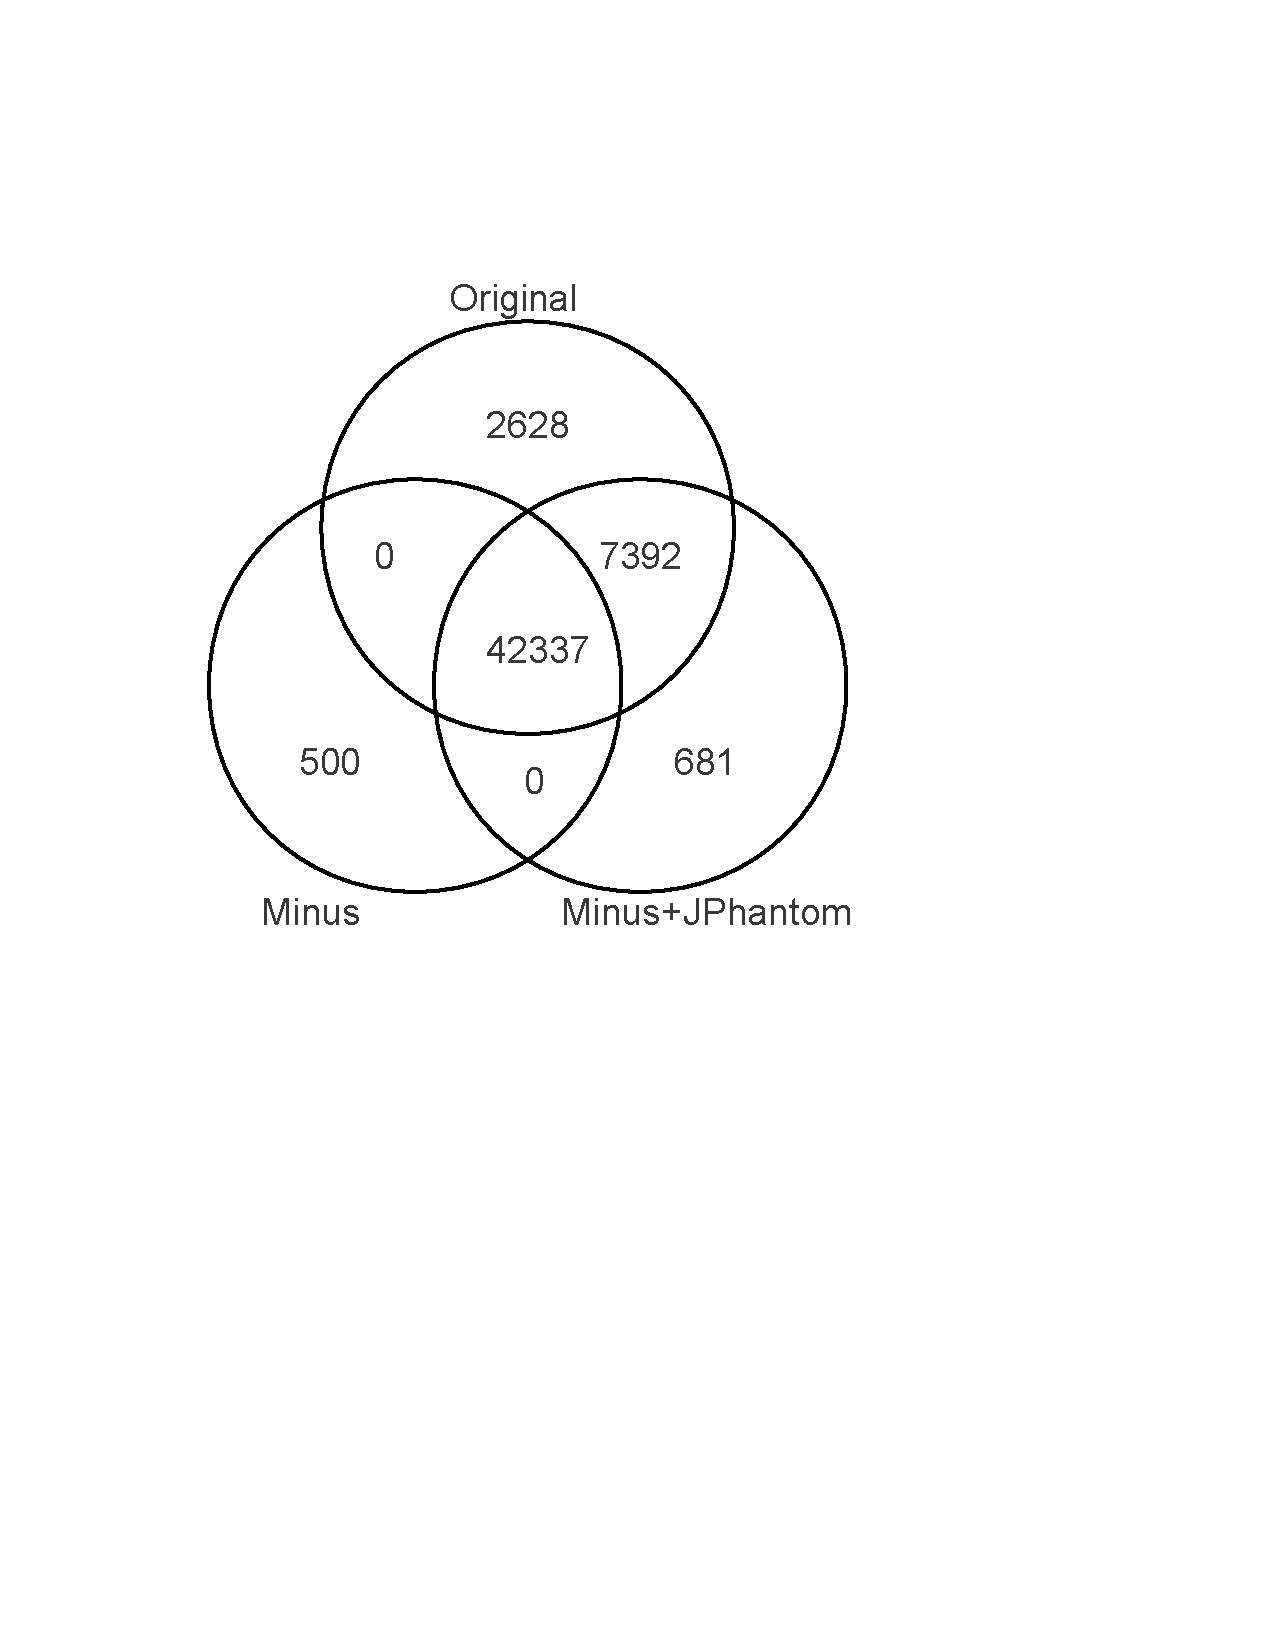
\includegraphics[scale=0.65]{figures/complementation/venn.pdf}
  \caption[Reachable Methods Venn Diagram]{ A Venn diagram that shows
    how three different sets of reachable methods relate to each
    other. These three sets---(i) \emph{Original}, (ii) \emph{Minus},
    and (iii) \emph{Minus+JPhantom}---correspond to the outcomes of
    analyzing (i) the \emph{antlr} jar (original), (ii) the
    \emph{antlr-minus} jar (subset of the original jar), and (iii) the
    \emph{antlr-minus} jar after being transformed by JPhantom,
    respectively. The sets are not drawn to scale: the size of each
    subset is indicated only by the number in it.}
  \label{hiercomp/fig:venn}
\end{figure}

In summary, JPhantom avoids problems with crashes when encountering
phantom references as well as incompleteness when phantom references
are merely ignored. In practice, it is effective in discovering large
parts of the interface for missing methods and the produced complement
respects the requirements of the Java VM verifier, i.e., the most
fundamental Java well-formedness rules for types.


\subsection{Performance Experiments}

We use a 64-bit machine with a quad-core Intel i7 2.8GHz CPU. The
machine has 8GB of RAM. We ran our experiments using JDK 1.7
(64-bit).

Our benchmarks consist of
\begin{inparaenum}[(1)]
\item \emph{antlr}, a parser generator,
\item \emph{antlrworks}, the GUI Development Environment for antlr,
\item \emph{c3p0}, a library that provides extensions to traditional
  JDBC drivers,
\item \emph{jruby} and
\item \emph{jython}, implementations of Ruby and Python programming
  languages respectively that run on top of the JVM,
\item logback-classic and
\item logback-core, two modules of the \emph{logback} logging
  framework,
\item \emph{pmd}, a Java source code analyzer,
\item \emph{postgres}, the PosgreSQL JDBC driver,
\item \emph{sablecc}, a compiler generator, and
\item \emph{antlr-minus}, a synthetic benchmark described in the
  previous section.
\end{inparaenum}
% in order to increase the number of constraints it produces.
Every benchmark is just a jar file that serves as JPhantom's
input, which then detects all phantom references and generates the
complemented jar.

We encountered most of these benchmarks in our own work doing static
program analysis with the \doop{} framework
\cite{oopsla/BravenboerS09,pldi/KastrinisS13}. For many of the
benchmarks it was, upon original encounter, an unexpected discovery
that they could not be analyzed due to dependencies to unknown classes
in other libraries.

Figure~\ref{hiercomp/fig:exp1} presents input features and the running time of
JPhantom for each of our benchmarks. The first column is the name of
the benchmark. The second column is the size of the output, i.e., the
complemented jar, divided into the original size of the input
(benchmark) and the size of the complement itself (i.e., the size of
the generated phantom classes). The third and fourth columns are the
number of phantom classes and constraints detected respectively. The
last column is the running time of JPhantom, including the time to
analyze the input, compute a type hierarchy that respects all of the
constraints detected, create the phantom classes with the required
members and supertypes, augment the input jar and flush its contents
to disk.

\begin{figure}
\centering
\small
\begin{savenotes}
\begin{tabular}{@{}l@{\hspace{1em}}r@{\ +\ }r@{\hspace{1em}}r@{\hspace{1em}}r@{\hspace{1em}}r@{}}
  \toprule
  %% \emph{Input jar} & \emph{Size} & \emph{Complement} &
  \emph{Input jar} & \multicolumn{2}{c}{\emph{Size}}  &
  \emph{Phantom} & \emph{Constraints} & \emph{Time} \\
  \midrule
  antlr & $3.3$M & $0.7$K & $1$ & $2$ & $4.82s$ \\ %% antlr-master-3.4.1-SNAPSHOT-completejar.jar (used to be 3.93)**
  antlrworks & $3.5$M & $2.2$K & $5$ & $7$ & $6.11s$ \\ %% antlrworks-1.5rc1.jar (used to be 5.12)
  c3p0 & $597$K & $1.8$K & $4$ & $2$ & $2.05s$ \\ %% c3p0-0.9.1.2.jar (used to be 1.86)
  jruby & $19$M & $5.9$K & $16$ & $20$ & $13.70s$ \\ %% jruby-complete-1.7.2.jar (used to be 12.06)
  jython & $2.5$M & $4.0$K & $8$ & $9$ & $3.26s$ \\ %% jython.jar (used to be 2.99)
  logback-classic & $247$K & $55$K & $148$ & $212$ & $1.76s$ \\ %% logback-classic.jar (used to be 1.55)
  logback-core & $358$K & $7.9$K & $22$ & $22$ & $1.61s$ \\ %% logback-core-1.0.9.jar (used to be 1.22)
  pmd & $1.2$M & $11$K & $28$ & $36$ & $2.62s$ \\ %% pmd.jar (used to be 2.25)
  postgres & $499$K & $0$ & $0$ & $0$ & $1.95s$ \\ %% postgresql-8.4-701.jdbc4.jar (used to be 1.56)
  sablecc & $306$K & $2.3$K & $5$ & $8$ & $1.59s$ \\ %% sablecc-3.2.jar (used to be 1.32)
  \midrule
  antlr-minus & $3.2$M & $17$K & $37$ & $103$ & $5.82s$ \\ %% antlr-final.jar (used to be 4.72)
  \bottomrule
\end{tabular}
\end{savenotes}
\caption{%
    Results of experiments.
}
\label{hiercomp/fig:exp1}
\end{figure}


%% The execution times presented above changed since we added an extra
%% pass to jphantom, to account for missing members of available
%% classes. That is, an available class may call a method or reference
%% a field declared in one of its supertypes. It may be the case that
%% the member was declared in a phantom supertype, and thus no
%% declaration for it exists in the available classes,
%% whatsoever. What we did is, try to perform a member lookup for any
%% reference of a type that has at least one phantom supertype. If the
%% lookup fails, we pick a phantom supertype and add a constraint
%% which states that this phantom supertype must declare the missing
%% member. To perform the lookup, we had to implement an extra pass
%% that stores all declared methods and fields of the available
%% classes.

Even the largest benchmark (jruby) takes seconds to
complete. Moreover, the size of the input is highly correlated with
the running time of JPhantom and much less correlated with the number
of constraints. This suggests that most of the time is spent on
reading and analyzing the input, rather than on the type hierarchy
solver. The only slight exception is the logback-classic benchmark,
which requires about 1.8 seconds to complete despite its small
size. This is due to the large number of phantom classes and
constraints this benchmark produces, which is to be expected since it
is built on top of logback-core (which is not supplied as part of the
input). This practice of creating such a strong dependency is probably
justified by logback's design. The framework implements the SLF4J
(Simple Logging Facade for Java) protocol, which acts as a common
interface for a variety of logging frameworks, and hides the actual
framework (called
\emph{binding}) to be used underneath. From both logback-classic and
antlr-minus we can see that JPhantom scales well as the number of
constraints increases.

To see the constraints and their solution for a benchmark instance,
consider the list below, which is the actual execution output of a
JPhantom run on the jruby benchmark:

\begin{alltt}\footnotesize
\vspace{2em}
Phantom Classes Detected: \hfill{[constraint]}

org.apache.tools.ant.BuildException \hfill{must be a class}
org.apache.tools.ant.Task \hfill{must be a class}
org.apache.tools.ant.Project
org.apache.bsf.util.BSFFunctions \hfill{must be a class}
org.apache.bsf.util.BSFEngineImpl \hfill{must be a class}
org.apache.bsf.BSFException \hfill{must be a class}
org.apache.bsf.BSFManager \hfill{must be a class}
org.apache.bsf.BSFDeclaredBean \hfill{must be a class}
org.apache.bsf.BSFEngine
org.osgi.framework.Bundle \hfill{must be an interface}
org.osgi.framework.BundleReference
org.osgi.framework.FrameworkUtil \hfill{must be a class}
org.osgi.framework.BundleException
org.osgi.framework.BundleContext \hfill{must be an interface}
java.dyn.Coroutine \hfill{must be a class}
java.dyn.CoroutineBase

Constraints:

org.apache.bsf.BSFException <: Throwable
org.apache.tools.ant.BuildException <: Throwable
org.osgi.framework.BundleException <: Throwable
org.jruby.embed.bsf.JRubyEngine <:
  org.apache.bsf.util.BSFEngineImpl
org.jruby.embed.bsf.JRubyEngine <:
  org.apache.bsf.BSFEngine
org.jruby.ant.RakeTaskBase <: org.apache.tools.ant.Task
org.jruby.javasupport.bsf.JRubyEngine <:
  org.apache.bsf.BSFEngine
org.jruby.ext.fiber.CoroutineFiber$1 <:
  java.dyn.Coroutine
org.jruby.javasupport.bsf.JRubyEngine <:
  org.apache.bsf.util.BSFEngineImpl

Class Hierarchy
* class java.lang.Object
  * class org.apache.bsf.BSFManager
  * class org.osgi.framework.FrameworkUtil
  * class Throwable (implements java.io.Serializable)
    * class org.osgi.framework.BundleException
    * class org.apache.tools.ant.BuildException
    * class org.apache.bsf.BSFException
  * class org.apache.bsf.BSFDeclaredBean
  * class org.apache.bsf.util.BSFFunctions
  * class org.apache.tools.ant.Task
    * class org.jruby.ant.RakeTaskBase
  * class java.dyn.Coroutine
    * class org.jruby.ext.fiber.CoroutineFiber$1
  * class org.apache.bsf.util.BSFEngineImpl (implements
     org.apache.bsf.BSFEngine)
    * class org.jruby.javasupport.bsf.JRubyEngine
    * class org.jruby.embed.bsf.JRubyEngine

Interface Hierarchy
* interface org.osgi.framework.Bundle
* interface org.apache.bsf.BSFEngine
* interface java.io.Serializable
* interface org.osgi.framework.BundleContext
\end{alltt}

It is evident that the final hierarchy respects all of the reported
constraints. Some interesting points are that:
\begin{inparaenum}[(i)]
\item \javaclass{org.apache.bsf.BSFEngine} defaults to interface since no
  constraint determines whether it is actually an interface or a
  class,
\item \javaclass{org.osgi.framework.BundleException} is inferred to be a
  class since it is a subtype of the class \javaclass{Throwable}, and
\item two known classes,
  \javaclass{org.jruby.javasupport.bsf.JRubyEngine} and
  \javaclass{org.jruby.embed.bsf.JRubyEngine}, used as subtypes of
  interface \javaclass{org.apache.bsf.BSFEngine}, add the latter to
  the supertypes of their phantom projection,
  \javaclass{org.apache.bsf.util.BSFEngineImpl}.
\end{inparaenum}


%-------------------------------------------------------------------------------
% Discussion
%-------------------------------------------------------------------------------

\section{Discussion}
\label{hiercomp/discussion}

We next discuss the problem of hierarchy complementation speculatively,
in settings different from ours. The general problem is that of
complementing programs so that they respect static well-formedness
requirements. Thus, the problem applies to language-level type
systems, static analyses (e.g., ``complement this program so that it
passes this analysis, defined a priori'') and other settings more
general than our Java bytecode domain. Indeed, much of our ability to
solve the problem effectively has to do with the simple type
checking performed by the Java bytecode verifier. The verifier
effectively checks monomorphic types, i.e., that a reference to an
object is statically guaranteed to refer to memory with the expected
layout.

If we were to transpose the problem to the domain of Java source code,
the constraints to be derived are richer and more complex than
the ones we encountered.
%\footnote{Complex constraints mean that the
%  problem can easily be shown to be NP-hard or worse.}
%: One can imagine
%  undecidable variants where a constraint can be satisfied only by
%  inventing ``new'' unknown types.}
The Java language-level type system has intricate requirements
relative to overriding, casts, exceptions, and more.  By way of
example, we discuss some of these complications below.

\begin{itemize}[--]
\item Exception handling at the Java language level immediately
  introduces very powerful constraints for types. The Java language
  requires that a method that overrides another may throw an exception
  only if it was already declared to be thrown. Consider two methods:

  \begin{javacode}
    class S {
      void foo() throws A, B {...}
    }

    class C  extends S {
      void foo() throws X, Y, Z {...}
    }
  \end{javacode}

  The requirement in this case is hard to reason about without an
  exhaustive search. It can be stated as: ``for \code{C.foo} to be a
  valid overriding of \code{S.foo}, \code{X}, \code{Y} and \code{Z}
  have to be subtypes of either \code{A} or \code{B}.''  Consider how
  this rich constraint would affect our ability to solve the hierarchy
  complementation problem at the source level. Imagine that \code{S}
  is a known class while \code{C}, \code{X}, \code{Y}, and \code{Z}
  are phantom classes. If the language allowed us to infer through
  observation of other code that \code{C} is a subtype of \code{S} and
  that it provides a method ``\code{void foo() throws X, Y, Z}'' then
  in order to generate a complement we would need to satisfy the
  following:
  $\code{C} <: \code{S} \Rightarrow \forall t \in \{\code{X,Y,Z}\}: (t
  <: \code{A} \lor t <: \code{B})$.

  % This kind of constraint expression immediately gives us the
  % ability to express disjunction subtyping constraints. Such
  % expressive constraints lead to intractable handling in the worst
  % case (e.g., it is easy to prove NP-hardness for the satisfiability
  % problem of this and other constraint kinds below).

  In contrast, the bytecode verifier only ensures a much simpler
  constraint: that a type declared to be thrown by a method is a
  subtype of \code{Throwable}.

\item A similar kind of constraint at the Java language level is also
  produced by the overriding rule for return types. Java (5 and above)
  allows overriding methods to have a covariant return type. That is,
  the overriding method can declare to return a subtype of the
  overridden method's return type. Much as in the case of exceptions,
  this induces complex constraints, especially when combined with
  search to examine whether a type can be a subtype of another.
  Consider the following case:

  \begin{javacode}
    interface S {
      R foo();
    }
    // R,X,Y phantom types
    // we know X contains method "Y foo()"
  \end{javacode}

  For phantom types \code{R} and \code{X}, if some other constraint
  (e.g., of the kind induced in the case of multiple inheritance in
  Section~\ref{hiercomp/multiple}) can be satisfied by making \code{X} a
  sybtype of \code{S}, then we get the additional constraint: ``if
  \code{X} becomes a subtype of \code{S} then \code{Y} must be a
  subtype of \code{R}''. This is again a very expressive constraint
  kind and, consequently, hard to reason about. For instance, the
  above constraint allows us to determine that two phantom types
  cannot be subtype-related. If two types declare methods with
  identical argument types but guaranteed-incompatible return types
  (e.g., \code{void} and \code{Object}), then the types are guaranteed
  to not be ordered by the subtyping relation, in either direction.

  At the bytecode level, subtyping together with signature conformance
  does not imply other subtyping relationships, in the above
  manner. By merely having a method with the same argument types, we
  are not guaranteed that it overrides the respective superclass
  method. Instead, overloading is perfectly legal among methods that
  differ only in their return types. The bytecode method call
  resolution procedure does not rely on name/type lookup but on direct
  identifiers of methods.

\item Casts yield no constraints at the bytecode level although they
  do at the source level. The reason is that the bytecode elides all
  unnecessary casts (i.e., upcasts). For instance, at the source
  level, upon seeing in code that passes the type checker a statement
  of the form ``\code{(X) new C()}'' we can be certain that (assuming
  \code{X} and \code{C} are both classes) the classes \code{X} and
  \code{C} are subtype-related: the cast can be either an upcast or a
  downcast, otherwise it would fail statically. At the bytecode level,
  however, a corresponding ``\code{checkcast X}'' instruction, when
  the object at the top of the argument stack is of static type
  \code{C}, allows no inference. The corresponding source code could
  well have been ``\code{(X)((Object) c)}'', with the intervening
  upcast elided during compilation to bytecode.

\item Constraints can be induced not just by varying the requirements
  for the output but also by varying the assumptions for the input.
  In our setting, we only assumed that the input is legal Java
  bytecode when complemented with some extra definitions. This is
  distinctly different from assuming that the input has been produced
  by the translation of Java source code. (Bytecode could well have
  been produced via compilers for other high-level languages or via
  bytecode generators.) For instance, the Java language maintains
  types for all local variables. At the source level, if we call
  methods on the outcome of a conditional expression, we are
  guaranteed to be able to assign a type to it. Consider:

  \begin{javacode}
    A a;
    B b;
    x = (foo()? a : b);
    x.meth();  // I::meth()
    x.meth2(); // J::meth2()
  \end{javacode}

  In Java source, the above code means that there exists some type
  \code{X} (the type given to variable \code{x}) such that \code{X} is
  a subtype of \code{I} and \code{X} is a subtype of \code{J}, while
  also \code{A} and \code{B} are subtypes of \code{X}. An equivalent
  conditional in bytecode form does not need to assign a type to
  \code{X}. The constraints will be merely: \code{A} and \code{B} are
  subtypes of both \code{I} and \code{J}, without allowing us to infer
  the existence of such an unknown type \code{X}. Our constraint
  solving process is significantly simplified by the fact that we
  never need to infer the existence of more types.

\end{itemize}

The above is just a sampling of complications that arise if the
hierarchy complementation problem is transposed to other domains,
requiring the satisfaction of different static requirements. The
effectiveness and efficiency of our approach is largely due to
the simplicity of the Java bytecode verification requirements.
However, other domains give rise to challenging problems,
with a wealth of different constraints, possibly appropriate for
future work.

%-------------------------------------------------------------------------------
% Conclusions
%-------------------------------------------------------------------------------

\section{Conclusions}

We introduced the class hierarchy complementation problem. The problem
consists of finding definitions to complement an existing partial
class hierarchy together with extra subtyping constraints, so that the
resulting hierarchy satisfies all constraints. In the context of Java
bytecode and the constraints of the bytecode verifier, our problem is
the core challenge of complementing partial programs soundly, i.e., so
that they pass the checks of the verifier when loaded together with
the generated complement. We offered algorithms for the hierarchy
complementation problem in both the single and the multiple
inheritance setting, and linked it to practice with our JPhantom
bytecode complementation tool.

We believe that the hierarchy complementation problem is fundamental
and is likely to arise in different settings in the future, hopefully
aided by our modeling of the problem and some of its solution avenues.



%%% Local Variables:
%%% mode: latex
%%% TeX-master: "../thesis"
%%% End:


\chapter{Related Work}
\label{chapter:related}
\epigraph{Obviously, you're not a golfer.}{\textit{The Dude}}

This chapter includes related work of previous chapters (in Sections
\ref{related:sect/structsens} -- \ref{related:sect/hiercomp})
and then considers more generic directions in static analysis
literature (in Section~\ref{related:sect/misc}).
%
Specifically,
\begin{inparaenum}[(a)]
\item Section~\ref{related:sect/structsens} contains related work for
  Chapter~\ref{chapter:structsens};
\item Section~\ref{related:sect/reflection} contains related work for
  Chapter~\ref{chapter:reflection}; and
\item Section~\ref{related:sect/hiercomp} for
  Chapter~\ref{chapter:hiercomp}.
\end{inparaenum}

\section{Field-Sensitive C/C++ Pointer Analysis}
\label{related:sect/structsens}

Regarding our structure-sensitive pointer analysis, we discussed some
closely related work throughout Chapter~\ref{chapter:structsens} (most
importantly \cite{paste/PearceKH04,toplas/PearceKH07}). More
generally, most C and C++ analyses in the past have focused on
scalability, at the expense of precision. Several (e.g.,
\cite{antgrasshopper,popl/ZhengR08,popl/Lhotak11}) do not model more
than a small fraction of the functionality of modern intermediate
languages.

One important addition is the DSA work of Lattner et
al.~\cite{pldi/LattnerLA07}, which was the original points-to analysis
in LLVM. The analysis is no longer maintained, so comparing
experimentally is not possible. In terms of a qualitative comparison,
the DSA analysis is a sophisticated but ad hoc mix of techniques, some
of which add precision, while others sacrifice it for scalability. For
instance, the analysis is field-sensitive using byte offsets, at both
the source and the target of points-to edges. However, when a single
abstract object is found to be used with two different types, the
analysis reverts to collapsing all its fields. (Our analysis would
instead create two abstract objects for the two different types.)
Furthermore, the DSA analysis is unification-based (a Steensgaard
analysis), keeping coarser abstract object sets and points-to sets
than our inclusion-based analysis. Finally, the DSA analysis uses deep
context-sensitivity, yet discards it inside a strongly connected
component of methods.
%Overall, the DSA
%analysis is intriguing and it would be interesting to compare its
%precision with our approach, 

The field-sensitive inclusion-based analysis of Avots et
al. \cite{icse/AvotsDLL05} uses type information to improve its
precision. As in this work, they explicitly track the types of objects
and their fields, and filter out field accesses whose base object has
an incompatible type (which may arise due to analysis
imprecision). However, their approach is array-insensitive and does
not employ any kind of type back-propagation to create more
(fine-grained) abstract objects for polymorphic allocation
sites. Instead, they consider objects used with multiple types as
possible type violations. Finally, they extend type compatibility with
a form of structural equivalence to mark types with identical physical
layouts as compatible. The implementation of \cclyzer{} applies a more
general form of type compatibility, presented in
Section~\ref{structsens/sect/addons}.

\citeauthor{lctrts/Mine06} \cite{lctrts/Mine06} presents a highly
precise analysis, expressed in the abstract interpretation framework,
that translates any field and array accesses to pointer arithmetic. By
relying on an external numerical interval analysis, this technique is
able to handle arbitrary integer computations, and, thus, any kind of
pointer arithmetic. However, the precision comes with scalability and
applicability limitations: the technique can only analyze programs
without dynamic memory allocation or recursion.
%(which commonly applies only to embedded critical software).

There are similarly other C/C++-based analyses that claim
field sensitivity~\cite{popl/HardekopfL09,cgo/HardekopfL11}, but it is
unclear at what granularity this is implemented. Existing descriptions
in the literature do not match the precision of our
structure-sensitive approach, which maintains maximal structure
information (with typed abstract objects and full distinction of subobjects), at
both sources and targets of points-to relationships. Nystrom et
al.~\cite{paste/NystromKH04} have a fine-grained heap abstraction that
corresponds to standard use of ``heap cloning''
(a.k.a. ``context-sensitive heap'').% techniques.


\section{Static Analysis and Java Reflection}
\label{related:sect/reflection}

The traditional handling of reflection in static analysis has been
through integration of user input or dynamic information.  The
Tamiflex tool~\cite{icse/BoddenSSOM11} exemplifies the state of the
art. The tool observes the reflective calls in an actual execution of
the program and rewrites the original code to produce a version
without reflection calls. Instead, all original reflection calls
become calls that perform identically to the observed execution. This
is a practical approach, but results in a blend of dynamic and static
analysis.
% Clearly, the greatest motivation for
%static analysis is to capture all possible program behaviors.
It is unrealistic to expect that uses of reflection will always yield
the same results in different dynamic executions---or there would be
little reason to have the reflection (as opposed to static code) in
the first place. Our approach attempts to restore the benefits of
static analysis, with reasonable empirical soundness.

An alternative approach is that of Hirzel et
al.~\cite{ecoop/HirzelDH04,toplas/HirzelDDH07}, where an online
pointer analysis is used to deal with reflection and dynamic loading
by monitoring their run-time occurrence, recording their results, and
running the analysis again, incrementally. This approach is quite
interesting when applicable. However, it is not applicable in many
static analysis settings. Maintaining and running a precise static
analysis during program run time is often not realistic (e.g., for
expensive context-sensitive analyses). Furthermore, the approach does
not offer the off-line soundness guarantees one may expect from static
analysis: it is not possible to ask questions regarding all methods
that may ever be called via reflection, only the ones that have been
called so far.

Interesting work on static treatments of reflection is often in the
context of dynamic languages, where resolving reflective invocations
is a necessity.  Furr et al.~\cite{oopsla/FurrAF09} offer an analysis
of how dynamic features are used in the Ruby language. Their
observations are similar to ours: dynamic features (reflection in our
case) are often used either with sets of constant arguments (in order
to avoid writing verbose, formulaic code), or with known
prefixes/suffixes (e.g., to re-locate within the file system).

Madsen et al.~\cite{sigsoft/MadsenLF13} employ a use-based analysis
technique in the context of Javascript. When objects are retrieved
from unknown code (typically libraries) the analysis infers the
object's properties from the way it is used in the client. In
principle, this is a similar approach to our use-based techniques
(both object invention and back-propagation) although the technical
specifics differ. The conceptual precursor to both approaches is the
work on reflection by Livshits et
al.~\cite{aplas/LivshitsWL05,livshits:thesis}, which has been
extensively discussed and contrasted throughout this chapter (see
Sections~\ref{reflection/sec:model}, and \ref{reflection/sec:use-based}).

Advanced techniques for string analysis have been presented by
Christensen et al.~\cite{sas/ChristensenMS03}. They analyze complex
string expressions and abstract them via a context-free grammar that
is then widened to a regular language. The regular approximations
produced by this approach are richer than the prefix and suffix
matching of our substring analysis, and can thus better approximate
the possible values of arbitrary string expressions. Reflection is one
of their examples but they only apply it to small benchmarks.

\citeauthor{ecoop/AliL12}~\cite{ecoop/AliL12,ecoop/AliL13} offer
comparisons of dynamic and static call-graph edge metrics.  They
discover hundreds of missing edges in several of the DaCapo
2006-10-MR2 benchmarks.  However, their experiments do not integrate
the vastly improved support for reflection (e.g., modeling of
\javasignature{Object.getClass}) offered by \textsc{Elf} or our
current work.

%were performed
%before numerous engineering improvements in the \textsc{Doop}
%framework.
%These improvements handle many common API calls, such as
%\javasignature{Object.getClass}.
%Furthermore, some benchmarks could not be run with reflection enabled
%due to scalability issues. Therefore, o
%%SPACE
%Our experiments are substantially more representative in regards to
%the actual empirical soundness of a joint reflection and pointer
%analysis.
Stancu et al.~\cite{pppj/StancuWBLF14} empirically
%present an empirical study that
compare profiling data with a points-to static analysis.
%,but do not support reflection.
However, they target only the most reflection-light benchmarks of the
DaCapo 9.12-Bach suite (\emph{avrora, luindex, and lusearch}), and
patch the code to avoid reflection entirely.

% TODO consider adding, after move
%Some of the most closely related work to ours is the Li et
%al. work~\cite{ecoop/LiTSX14}, discussed earlier. Li et al. also
%improve on the engineering aspects of reflection handling in the
%\textsc{Doop} framework, as well as employ a back-propagation
%technique. The work is concurrent to ours and we have only been able
%to obtain a preprint at the time of this writing. Nevertheless, the
%differences of the two approaches seem quite clear, as also discussed
%in Section~\ref{reflection/sec:back-propagation}. Furthermore, the Li et al.
%technique does not employ substring matching or substring flow
%analysis and does not emphasize empirical soundness. Instead it
%eagerly under-approximates many more reflective calls and resolves
%such calls only when forward and backward reflection analysis
%information agrees. A valuable aspect of the Li et al. work is a
%detailed study of how reflection is used in practical programs.


\section{Class Hierarchy Complementation and Static Analysis on
  Partial Programs}
\label{related:sect/hiercomp}

The hierarchy complementation problem is in principle new, although
indirectly related to various other pieces of work in the literature.

From a theory standpoint, our problem is an attempt to more fully
determine the structure of a partially ordered set. There is no exact
counterpart of our algorithms in the literature. However, there has
been work on sorting a poset, i.e., completely determining the partial
order \cite{soda/DaskalakisKMRV09}.  The challenge in such algorithmic
research, however, is to perform the sorting with a minimal number of
queries. None of the interesting devices of our algorithms are
present. Specifically, the device of the single inheritance case (if a
node can reach two others, they have to be ordered relative to each
other) does not apply, and neither does the interesting constraint of
the multiple inheritance case (we cannot add direct supertypes to a
known node).

Complementing a program so that the result respects static properties
is analogous to analyzing only parts of a program but giving
guarantees on the result. There are few examples of program analyses
of this nature. Notably, \citeauthor{ecoop/AliL12} recently introduced
a technique \cite{ecoop/AliL12} for analyzing an application
separately from a library, while keeping enough information (from the
library analysis) to guarantee that the application-level call-graph
is correct. Furthermore, the Averroes system \cite{ecoop/AliL13} uses
the assumption that the missing code is independently developed in
order to produce a worst-case skeletal library. That is, Averroes
takes an existing library and strips away the implementation, keeping
only the interface between the library and the application. The
implementation is replaced with code (at the bytecode level) that
performs worst-case actions on the arguments passed into the library,
for the purposes of call-graph construction (i.e., the generated code
calls all methods the eliminated original code could ever
call). Averroes is related to JPhantom but at rather opposite ends of
the spectrum: Averroes produces worst-case skeletal implementations,
while JPhantom produces minimal, best-case implementations that still
respect well-formedness at the type level.  At the same time, Averroes
assumes the library interface is available and just tries to avoid
analyzing library implementations, while JPhantom applies precisely
when the library is completely missing. Thus, JPhantom truly applies
to the case of partial programs, whereas Averroes analyzes a partial
program but under the assumption that the whole program was available
to begin with. It would be interesting to treat a partial program
first with JPhantom and then apply Averroes to the JPhantom-produced
program complement to obtain the worst-case behavior of a plausible
interface for the missing code.

Analyzing partial programs at the level of source code has been
studied by \citeauthor{oopsla/DagenaisH08}
\cite{oopsla/DagenaisH08}. Apart from the elaborate type constraints
that may arise from missing source code, as discussed in
Section~\ref{hiercomp/sect/discussion}, another important challenge is
syntactic ambiguities (e.g., \emph{is it a package or a class
  name?}). The goal of \citeauthor{oopsla/DagenaisH08} is to be able
to deal with both typing problems and syntactic ambiguities in any
given partial Java program and produce a typed IR (although it may
contain placeholders representing unknown types and packages). Their
approach is primarily based on heuristics that make arbitrary choices
on various occasions (with no form of backtracking) that may
eventually lead to wrong results. Even though they, too, identify
similar subtype constraints and record missing class members to be
added in the typed IR, they do not define any similar type hierarchy
complementation problem or come up with algorithms to systematically
construct a valid solution in such a setting.

% - deal with syntactic ambiguities as well as typing problems
% - builds a typed IR (typed AST and Jimple) from a partial program with
%   no unknown syntactic constructs
% - share subtype constraints and adding missing class members
% - no backtracking, heuristic-based approach
% - heuristics make arbitrary choices that may produce wrong results
% - may yield unknown type and package placeholders

Our hierarchy complementation problem bears a superficial resemblance
to the \emph{principal typings} problem
\cite{popl/AnconaZ04,popl/AnconaDDZ05,Ancona04even}.  The principal
typings problem consists of computing types for a Java module in
complete isolation from every other module it references. I.e.,
principal typings aim to achieve a more aggressive form of separate
compilation, by computing the minimal type information on other
classes that a class needs in order to typecheck and compile. Thus,
the motivation is fairly similar to ours, but the technical problem is
quite different.  First, in our setting we already have the result of
compilation in the form of bytecode, and bytecode only. Second, our
emphasis is on satisfying constraints instead of capturing them as a
rich type. Finally, our constraints are of a very different nature
from any in the principal typings literature. As discussed in
Section~\ref{hiercomp/sect/discussion}, the input and output language
assumptions crucially determine the essence of an incomplete program
analysis problem.



\section{Other Directions in Static Analysis}
\label{related:sect/misc}

%% -----------------------------------------------------------------------------
%   CFL Reachability Problems
%% -----------------------------------------------------------------------------

\paragraph{CFL reachability formulation.} In
Chapter~\ref{chapter:structsens}, we formulated pointer analysis
algorithms in Datalog. Employing a restricted language not only offers
guarantees of termination and complexity bounds, but also permits more
aggressive optimization of the language features.

Along these lines, pointer analysis and other related analyses have
been formulated as a \emph{context-free language (CFL) reachability}
problem. The idea is that we may encode an input program as a labeled
graph, and a specific analysis corresponds to the definition of a
context-free grammar, \(G\). The relation being computed holds for two
nodes of the graph if and only if there exists a path from one node to
the other, such that the concatenation of the labels of edges along
the path belongs in the language \(L(G)\) defined by \(G\).

Specifically, the input graph normally consists of nodes representing
program elements such as variables, types, methods, statements, and so
on. Edges represent relations between those program elements. For
instance, an edge \((s,\,t)\) may represent that there exists an
assignment from variable \(s\) to variable \(t\). Moreover, edges may
encode field accesses (load/store), method invocations, pointer
dereferences, etc, and hence may even connect different \emph{kinds}
of program elements. The exact choice of domains depends on the
specific analysis being run and the problem it addresses. Since we
want to express many input relations, we need many types of edges,
represented as labels (e.g., we can label a field access edge by some
symbol denoting field access plus the name of the field).  For a given
analysis, a context-free grammar \(G\) encodes the desired computed
relations (e.g., which pointers are memory aliases) as non-terminal
symbols, and supplies production rules that express how they relate to
the simpler relations represented by graph edges (terminals). The CFL
reachability answer is then commonly computed by employing a dynamic
programming algorithm.

The first application of such a framework in program analysis was
designed to solve various interprocedural dataflow-analysis problems
\cite{popl/RepsHS95}, but CFL reachability has since been used in a
wide range of problems, such as:
\begin{inparaenum}[(i)]
\item the computation of points-to relations
  \cite{journals/infsof/Reps98},
\item the (demand-driven) computation of may-alias pairs for a C-like
  language \cite{popl/ZhengR08},
\item Andersen-style pointer analysis for Java
  \cite{oopsla/SridharanGSB05}.
\end{inparaenum}

Any CFL reachability problem can be converted to a Datalog program
\cite{journals/infsof/Reps98}, but the inverse is not true (i.e., CFL
reachability corresponds to a restricted class of Datalog programs,
the so-called ``chain programs''). Thus, the primary advantage of CFL
reachability is that it permits more efficient implementations.

A \emph{chain program} consists of rules of the form:

\[p(X, Y) \leftarrow q_0(X,Z_1),\, q_1(Z_1, Z_2),\, \dots,\, q_k(Z_k,
  Y). \]

We can express a CFL reachability problem in Datalog by using such a
chain rule to represent the following production of grammar \(G\):

\[p \rightarrow q_0\; q_1\; \dots\; q_k \]

where a Datalog fact \(e(m, n)\) represents an edge \((m, n)\) labeled
\(e\) in the graph.

An even more restrictive variant, \emph{Dyck-CFL reachability}, can be
obtained by restricting the underlying CFL to a Dyck language, i.e.,
one that generates balanced-parentheses expressions. Although
restrictive, this approach still suffices for some simple pointer
analysis algorithms, while allowing very aggressive optimization,
often with impressive performance gains \cite{pldi/ZhangLYS13}.

% -CFL formulations (Dyck-CFL PLDI'13, Rugina, Bodik)
% \citep{pldi/ZhangLYS13}             % fast Dyck-CFL
% \citep{popl/ZhengR08}               % demand-driven; may-alias pairs
% \citep{journals/infsof/Reps98}      % also published in SLP' 1997; points-to relations
% \citep{popl/RepsHS95}               % interprocedural dataflow-analysis problems
% \citep{cc/Reps94}                   % magic-sets transformation -> demand-driven
% \citep{oopsla/SridharanGSB05}       % Java; demand-driven; balanced parentheses (field accesses)



%% -----------------------------------------------------------------------------
%   Shape Analysis
%% -----------------------------------------------------------------------------

\paragraph{Shape Analysis.}

So far, the techniques we have presented for pointer analysis have
been based on the allocation sites as the primary source for inventing
new abstract objects in memory. Despite our deviation from the
standard allocation-site abstraction, where a single abstract object
will be allocated per allocation site, even our own techniques
described in Chapter~\ref{chapter:structsens} will use the allocation
site as the basis of abstraction (but may create multiple objects per
site, nonetheless). A different approach altogether is that of the
techniques termed as \emph{shape analysis}
\cite{toplas/SagivRW02,popl/SagivRW99,sas/ManevichSRF04,sas/Lev-AmiS00,toplas/SagivRW98,sefm/FerraraFJ12}.
The primary goal of standard shape analysis is to be able to infer the
\emph{shapes} of objects in memory. E.g., to be able to detect if some
objects form a list or a tree, if some list may contain cycles, if a
subtree or a portion of a list may be shared (i.e., be reachable from
multiple objects), and so on.\footnote{The term shape analysis is
  quite generic (i.e., any analysis designed to infer the shapes of
  objects) and has been examined in many different contexts
  \cite{popl/GhiyaH96}. Here, we focus on \emph{parametric shape
    analysis via 3-valued logic}, as one of the most notable
  methodologies in that area.}

To achieve such a feat, shape analysis associates a list of properties
to each abstract memory object (e.g., \emph{pointed by variable
  \var{v}}, \emph{transitively reachable by variable \var{r}}, and so
on) and uses Kleene's three-valued logic to differentiate between must
and may information. For instance, if the ``\emph{pointed by variable}
\(\var{v}\)'' property of an abstract object \(\alloc{obj}\) has the
value 1 at some memory state, it means that variable \var{v}
\emph{must} point to this object (at the given state), whereas the
value \(1\over{2}\) would represent our familiar \emph{may} notion of
points-to. Hence, shape analysis performs an amalgam of must and may
analysis simultaneously.

At each memory state the analysis has computed, it tries to collapse
\(1\over{2}\) values of properties to either 0 or 1, via the so called
\emph{focus operation}. Inconsistent states are then discarded at the
\emph{coerce operation}. Thus, the analysis dynamically tries to
eliminate uncertainty by \emph{focusing} on the values of some core
predicates (and statement-specific formulas), at the expense of
possible memory state explosion---the abstract interpretation of each
program statement tends to create multiple output states for each one
of its input states.  As for abstract objects, they are defined only
by the values they have for some basic properties (called
\emph{abstraction properties}) of the particular analysis. Therefore,
the upper bound for the number of abstract objects in memory is
exponential with respect to the number of abstraction predicates
defined. The latter will almost certainly include a predicate per each
program variable.

By applying these techniques, and choosing the right abstraction
predicates, the analysis will be able to carve out the \emph{shapes}
of objects in memory. For instance, given an input memory state where
variable \var{v} points to the head of some list \(l\) with at least
two elements, the abstract interpretation of instruction ``\code{v =
  v->next}'' will create multiple output memory states where either:
\begin{inparaenum}[(i)]
\item \var{v} points to a new head of a list with a non-empty tail
  (corresponding to the case where \(l\) contained at least three
  elements), or
\item \var{v} points to the single element of a list with no tail at
  all (corresponding to the case where \(l\) contained exactly two
  elements).
\end{inparaenum}
In both output memory states, the analysis will compute values of 1
for the predicate ``\emph{pointed by variable \var{v}}''; hence, it
will know exactly where \var{v} points to and not lose any precision,
at the expense of increasing the possible memory states by 1.

\citeauthor{popl/SagivRW99} initiated the field of parametric shape
analysis via 3-valued logic
\cite{toplas/SagivRW98,popl/SagivRW99,toplas/SagivRW02}, and
\citeauthor{sas/Lev-AmiS00} presented the TVLA framework for shape
analysis \cite{sas/Lev-AmiS00}. Since then, there has been work on
various extensions such as
\begin{inparablank}
\item a more economic heap abstraction \cite{sas/ManevichSRF04},
\item better support for recursive programs \cite{cc/RinetzkyS01}
\item and programs with highly nested data structures
  \cite{cav/BerdineCCDOWY07} , and
\item the incorporation of a value analysis into the shape analysis
  algorithm~\cite{sefm/FerraraFJ12},
\end{inparablank}
among others.


%% -----------------------------------------------------------------------------
%   Separation Logic
%% -----------------------------------------------------------------------------

\paragraph{Separation Logic.}
Points-to analysis provides a model of the heap (or of memory in
general, for a language such as C). Other approaches for heap analysis
that can be used to prove pointer safety are based on the field of
\emph{separation logic}. Separation logic, in turn, can be viewed as
an extension of Hoare logic
\cite{journals/cacm/Hoare69,floyd1967assigning,lics:2002/Reynolds,csl/OHearnRY01}.
Hoare logic is a formal system for reasoning about the correctness of
programs, by encoding the programming language's semantics in
\emph{Hoare tiples}. A Hoare triple has the form \(\{P\}\, C\, \{Q\}\)
and describes how the execution of a command changes the state of the
computation. Specifically, it states that whenever the assertion \(P\)
holds, before executing command \(C\), then assertion \(Q\) will hold
afterwards (if \(C\) terminates). The \(P,\, Q\) assertions can
express conditions on program variables, written by using standard
mathematical notations together with logical operators (or, in
general, some form of calculus like \emph{first-order logic}).

Hoare logic provides two ways to generate verification conditions:
\begin{inparaenum}[(i)]
\item either forwards, by starting from a precondition and
  generating formulas to prove a postcondition
\item or backwards, by starting from a postcondition and trying to
  prove a precondition.
\end{inparaenum}
Either way, in the general case, it cannot provide fully automated
reasoning; building a proof may require human guidance.

% Even though there has been effort in increasing the level of
% automation (e.g., for the (semi-)automatic inference of loop
% invariants)

Separation logic
\cite{lics:2002/Reynolds,csl/OHearnRY01,popl/IshtiaqO01,Reynolds00intuitionisticreasoning}
extends Hoare logic by introducing additional operators in the syntax
of assertions, that facilitate local reasoning. Namely, the
\emph{separating conjunction} \(\,P * \,Q\) asserts that \(P\) and
\(Q\) hold for separate portions of memory, and thus can be used on
program-proof rules to provide modular reasoning about
programs. Additional operators include the separating implication,
\(P \sep Q\), which asserts that if the current heap is extended with
a disjoint part in which \(P\) holds, then \(Q\) will hold in the
extended heap, and more. Note that, these operators do not increase
the ``completeness'' of Hoare logic---what can be proven in separation
logic can also be proven in Hoare logic. Rather, they merely simplify
the specifications and proofs.

% citation needed
% Peter O'Hearn
% A Primer on Separation Logic (and Automatic Program Verification and Analysis)

\citeauthor{popl/CalcagnoDOY09} present a compositional shape analysis
\cite{popl/CalcagnoDOY09} to be used in (lightweight) program
verification that builds on these concepts of separation logic
(instead of the TVLA approach of \citeauthor{popl/SagivRW99}). In
classical logic, \emph{abduction} stands for the inference of
``missing'' assumptions \(M\), such that, given another assumption
\(A\) and a goal \(G\), one can prove \(G\) by synthesizing \(A\) and
\(M\):
\[A \,\land M\, \;\vdash\; G \]

A similar problem can be phrased by using separating conjunction
instead of classical conjunction, which also partitions the premises:
\[A \;*\; ??\, \;\vdash\; G \]

This finally leads to the more general problem of \emph{bi-abduction},
if we allow for leftover portions of state (the frame):
\[A \,*\, \textit{?anti-frame} \;\vdash\; G \,*\, \textit{?frame} \]

The notion of bi-abduction is used as the basis of a new compositional
interprocedural shape analysis algorithm.



%%% Local Variables:
%%% mode: latex
%%% TeX-master: "../thesis"
%%% End:


\chapter{Conclusions and Future Work}
\label{chapter:conclusions}
\epigraph{That rug really tied the room together.}{\textit{The Dude}}

In the final chapter, we shall assess our initial thesis and conclude,
while also considering interesting directions for future work.

Our thesis states that there exists \emph{implicit structural
  information} in the program, about the memory it will allocate,
which we can recover via inference and use it to improve the quality
of a static analysis (by coming up with a better abstract memory
model). In Chapter~\ref{chapter:structsens}, we examined the problem
of pointer analysis in C/C++, as a typical example of a low-level
language with direct memory access. We identified particular causes of
analysis imprecision, in untyped allocations (via generic
\code{malloc}-like allocation routines) and in the language's
capability of allowing pointers to point \emph{inside} an object
(i.e., to point to one of its fields or array elements), which further
complicates the modeling of field sensitivity.

We presented a structure-sensitive pointer analysis that may achieve
better precision by changing its abstraction strategy: when the same
allocation site is used to create objects of many different types, the
analysis comes up with many different strongly-typed abstract objects
to represent the same instruction. Also, each different field and
array element of each such strongly-typed object (of a complex type)
will be represented by a unique abstract subobject itself, having its
own separate points-to set, while also maintaining strong type
information. The final outcome is a much finer-grained allocation
abstraction (than that of the typical C/C++ points-to analysis) that is
guided primarily by the flow of types. The key to this technique is
that tracking the flow of types that will determine what objects will
be created is not determined before the analysis has run, but
simultaneously (``on-the-fly''), thus yielding better results due to
the recursive nature of the computation. We describe the analysis in
precise terms and show that its approach succeeds in maintaining
precision when analyzing realistic programs.

This is a prime example of how complex inference (in this case, the
relations computed by the pointer analysis itself) that tracks the use
of types in the program can be used to recover structural information,
namely, the various structures that may be used to access or modify
any untyped heap allocation in memory. The recovered structural
information, in turn, improves the quality of the analysis, in terms
of precision, as shown in the evaluation section of
Chapter~\ref{chapter:structsens}. In our experience, the techniques we
described are essential for analyzing C/C++ programs at the same level
of precision as programs in higher-level languages.

In Chapter~\ref{chapter:reflection}, we shift our focus to
higher-level languages like Java, with no pointer arithmetic or direct
memory access capabilities. However, even in such a setting, our thesis
applies: we can improve the quality of a pointer analysis (now, in
terms of empirical soundness) by recovering structural information for
objects involved in reflective operations. By using reflection, Java
programs can encompass dynamic behavior, and as such, are difficult to
statically analyze.

The challenges with reflection idioms are quite similar to those of
analyzing C/C++ that we have already encountered:
\begin{itemize}[\(\cdot\)]
\item the same (reflective) allocation site can be used to allocate
  objects of many different types
\item no local type information exists for reflective objects;
  instead, the types are determined by run-time strings that are passed
  on as arguments to the reflective operations involved
\item apart from normal object allocations, there are also reflective
  calls that return special objects representing program classes,
  fields, and methods; a reflective call on a method object is much
  like a C/C++ call via a function pointer.
\end{itemize}

To tackle the limitations of existing pointer analyses, induced by
reflection, we presented a static reflection analysis (which also runs
simultaneously with the core points-to analysis) that employs similar
techniques to those of Chapter~\ref{chapter:structsens}: by inspecting
the use of reflective objects (i.e., what types they are cast to, what
fields they access, and so on), the analysis is able to recover
essential parts of the objects' structure. Our techniques build on top
of state-of-the-art handling of reflection in Java, by elegantly
extending declarative reasoning over reflection calls and
inter-procedural object flow. Our main emphasis has been in achieving
higher empirical soundness, i.e., in having the static analysis truly
model observed dynamic behaviors.

By comparing the statically computed call-graphs against dynamically
computed ones from actual executions, we find that these techniques,
indeed, improve empirical soundness (i.e., the static analysis is now
able to cover more of the actual dynamic behavior of the program than
before). Although full soundness is infeasible for a realistic
analysis, it is possible to produce general techniques that enhance
the ability to analyze reflection calls.

As already noted, reflection is but one of the possible causes of lost
memory structure, when statically analyzing Java programs. In
Chapter~\ref{chapter:hiercomp}, we examine how to recover lost
structural information for partial Java programs.

% Static whole-program analysis requires the availability of every class
% transitively referenced in a program, even if it is never used. For
% instance, trying to analyze a program P that uses a small part of a
% third-party library L also requires the full code of any library L'
% that different parts of L may reference---the fact that L' is not
% necessary for P cannot be determined before the analysis of P is
% performed. This is a oft-encountered practical challenge, motivating
% mechanisms such as the ``phantom class'' facility in the well-known
% Soot analysis framework for Java.

Regarding such need, dynamic class loading allows programs to depend
on an abundance of external libraries, without actually requiring all
of them to execute. Transitive dependencies (i.e., the dependencies of
the libraries directly used by the program) make things even worse,
from the perspective of a static analyzer, since such dependencies are
much more numerous and less likely to be actually used. Hence, whole
programs might be both prohibitively difficult to obtain and
unnecessary at the same time; if some parts of the program were
missing, they would make no difference in any actual execution, had
these parts been truly redundant. In such cases, missing these parts
should also make no difference in analyzing the program, which
explains why there is a strong incentive for static analysis tools to
be able to analyze partial programs. Despite such incentive, static
analysis tools are rarely well-equipped or error-tolerant enough to be
able to cope with partial programs. When they do so, they risk a great
deterioration of their results.

% To address this challenge in full generality we define the problem
% of ``program complementation''
To this end, we have presented a generic complementation approach, in
Chapter~\ref{chapter:hiercomp}, that transforms a partial program to a
whole one, while also seeking to provide definitions for its missing
parts so that the ``complement'' satisfies all static and dynamic
typing requirements induced by the code under analysis. This requires
satisfying constraints relative to methods and fields of the missing
classes, as well as subtyping constraints and constraints on whether a
missing type has to be a class or interface.
%
To identify such constraints, we analyze the program and track uses
of any phantom types therein (i.e., types being used but not defined
in the code that is available), so that we can recover their
lost structure. Inferring missing members of phantom types is
straightforward. The primary challenge, however, lies in computing the
missing parts of the type hierarchy, in a way that satisfies all the
implied subtyping constraints.

We have defined the type hierarchy complementation problem as follows:
given a partially known hierarchy of classes together with subtyping
constraints (``A has to be a transitive subtype of B'') complete the
hierarchy so that it satisfies all constraints. We formulate the
problem systematically and offer algorithms to solve it in various
inheritance settings. The result is the articulation of a novel typing
problem in the OO context.

The entire complementation approach, including the algorithms to solve
the type hierarchy complementation problem are implemented in
JPhantom, a program complementation tool of practical interest for
Java bytecode.
%
We evaluated JPhantom on both synthetic and real-world benchmarks to
show that we produce practical complements of significant size in a
few seconds and, in this way, allow the analysis of previously
un-analyzable partial programs.

Lastly, we used the synthetic benchmark (based on the \emph{antlr}
parser generator) to evaluate the difference between analyzing a
partial program as is, and analyzing it after being complemented by
JPhantom. The comparison demonstrated that the latter is much closer
to analyzing the original whole program: analyzing the partial program
without complementation fails to find a great number of reachable
methods (which will not be analyzed at all). Therefore, recovering the
structural information of phantom types, via our program
complementation technique, has improved the static analysis on the
partial program, thus reinforcing our thesis.

We believe that the hierarchy complementation problem is fundamental
and is likely to arise in different settings in the future, hopefully
aided by our modeling of the problem and some of its solution avenues.

To summarize, we advocate that there are many opportunities of
recovering implicit structural information about memory that can
improve the static analysis of programs, but require complex inference
that takes advantage of indirect uses of types. We have examined three
different scenarios to test and evaluate our thesis, regarding
\begin{inparablank}
\item generic C/C++ programs, and
\item Java programs that either use reflection or
\item are missing parts of their code.
\end{inparablank}
In all cases, we where able to improve static analysis, by recovering
memory structure that was not previously evident.

% Highly dynamic features, such as reflection and dynamic loading, are
% the bane of static analysis. These features are not only hard to
% analyze well, but also ubiquitous in practice, thus limiting the
% practical impact of static analysis.

% +-----------------------------------------------------------------------------
% |  Future Work
% +-----------------------------------------------------------------------------

\section{Future Work}

Finally, we will discuss some interesting future directions to tackle
existing limitations of our approaches.

\subsection{Flow-Sensitivity and Strong Updates}

To begin with, our structure-sensitive points-to analysis for C/C++
lacks flow sensitivity, which is a useful feature for C-like
languages. Flow sensitivity takes the order of program instructions
into account, to increase analysis precision. The results it computes
are now specialized to a specific program point, at which they
hold. Thus, different program points will be associated with different
points-to results, by the end of an analysis run.

We have already discussed, in Chapter~\ref{chapter:structsens}, the
SSA transformation built in the LLVM bitcode format. SSA can be viewed
as a limited form of flow sensitivity, since it ensures that a
variable is only assigned once; a variable with multiple assignments
will be split into multiple different variables, one per assignment.
However, SSA is far from adequate, especially in LLVM bitcode, where
address-taken variables bypass SSA, by being transformed to pointers
whose contents can be changed by multiple store instructions. This is
not specific to analysis of C/C++ or LLVM bitcode. In a Java pointer
analysis, like the one we have briefly presented in
Chapter~\ref{chapter:reflection}, despite SSA, fields of objects can
be, again, updated multiple times.

To take advantage of flow sensitivity and be able to substantially
affect precision, an analysis has to perform \emph{strong updates}. A
store instruction strongly updates the results of an over-approximate
pointer analysis, when it overwrites the previous points-to contents
for the given address. A weak update only \emph{extends} points-to
contents without removing any prior results. However, it is not
generally sound for a flow-sensitive pointer analysis to perform a
strong update without additional reasoning. The reason is that an
abstract object summarizes multiple concrete objects; to strongly
update it, we have to ensure that the update applies to all concrete
objects that it represents.

We previously discussed how the recency-abstraction of
\citeauthor{sas/BalakrishnanR06}~\cite{sas/BalakrishnanR06} allows us
to perform strong updates.
%
Another approach is that of \citeauthor{popl/Lhotak11}, who perform
strong updates only on singleton points-to sets
\cite{popl/Lhotak11}.
%
However, even with strong updates, the cost of flow-sensitivity could
be prohibitive. Improving the efficiency of flow-sensitive analyses
has been studied extensively in the literature
\cite{sigsoft/LiCK11,sigsoft/SuiX16,ecoop/DeD12,iwmm/LiCK13}.
%
\citeauthor*{sas/KhedkerMR12} perform a context-sensitive and
flow-sensitive analysis but limit the points-to information they
compute based on a liveness analysis about pointer ranges
\cite{sas/KhedkerMR12}.
%
\citeauthor*{sas/YeSX14} limit flow-sensitivity by partitioning the
program into regions and maintaining flow-sensitivity only between the
regions but not inside \cite{sas/YeSX14}.
%
Incorporating such approaches and possibly devising other methods that
enable strong updates in limited cases would be a key step in
further improving the precision and overall value of our
structure-sensitive analysis.


\subsection{Integer and String Value Analysis}

Our structure sensitive analysis for C/C++ takes array indices into
account, to introduce a form of array-sensitivity by which it can
statically differentiate distinct array elements. Array indices are not
the only case where our analysis could benefit from integer values. The
number of bytes specified in an allocation instruction (e.g., via the
single parameter of a \code{malloc()} call) could help us filter some
invalid object-type associations.

Such cases, however, are only the tip of the iceberg in how a static
analysis can find use in reasoning about the domains of integer
values. Our analysis could incorporate more sophisticated approaches
in tracking integer-valued quantities and numerical properties of
program variables. For a language like C, which allows pointers to be
treated as integers, even aliasing information could be tied to
the computation of integer value domains. The standard use case of
numeric domains, however, is for answering queries about integer overflows
and array bounds checking.
%
One of the most precise approaches in the computation of numeric
abstract domains is the polyhedral domain
\cite{popl/CousotH78}. Cheaper variants include
\begin{inparablank}
\item the Octagons abstract domain~\cite{journals/lisp/Mine06},
\item the Pentagons domain~\cite{sac/LogozzoF08},
\item and difference-bound matrices (or Zones)~\cite{pado/Mine01}.
\end{inparablank}

For similar reasons, we can employ more sophisticated string analyses
to upgrade our reflection handling of
Chapter~\ref{chapter:reflection}, such as that of
\citeauthor*{sas/ChristensenMS03}~\cite{sas/ChristensenMS03}, which we
discussed in the previous chapter.


\subsection{Context Sensitivity}

We have already discussed context sensitivity in the previous section,
and the various strategies in specifying what program elements will
constitute the context.

For the analysis of LLVM bitcode---or any other format that has been
lowered to a C-like language for that purpose, where the OO features
have been translated away to more basic constructs---it is not evident
when and how to use object sensitivity in a generic and parameterized
way, such as the one proposed by \citeauthor*{popl/SmaragdakisBL11}
\cite{popl/SmaragdakisBL11}. Generalizing such approaches to work well
both in the presence and absence of object-oriented features, e.g., by
identifying what parameters could be used as objects, per method call,
is a direction worth investigating.



%%% Local Variables:
%%% mode: latex
%%% TeX-master: "../thesis"
%%% End:



%%%%%%%%%%%%%%%%%%%%%%%%%%%%%%%%%%%%%%%%%%%%%%%%%%%%%%%%%%%%%%%%%%%%%%%%%%%%%%%%
%%%%%%%%%%%%%%%%%%%%%%%%%%%%%%%   Back Matter  %%%%%%%%%%%%%%%%%%%%%%%%%%%%%%%%%
%%%%%%%%%%%%%%%%%%%%%%%%%%%%%%%%%%%%%%%%%%%%%%%%%%%%%%%%%%%%%%%%%%%%%%%%%%%%%%%%

\backmatter

%------------------------------------------------
% Abbreviations Table
%------------------------------------------------

\abbreviations
\begin{center}
	\renewcommand{\arraystretch}{1.5}
	\begin{longtable}{ l @{\qquad} l }
      \toprule
      % \emph{Abbrev} & \emph{Description} \\
      % \midrule
      ABI      & Application Binary Interface \\
      API      & Application Programming Interface \\
      CFL      & Context-Free Language \\
      DAG      & Directed Acyclic Graph \\
      DLL      & Dynamic-link Library \\
      GEP      & LLVM Bitcode's \code{getelementptr} instruction \\
      GUI      & Graphical User Interface \\
      DSA      & Data Structure Analysis \\
      IDE      & Integrated Development Environment \\
      IR       & Intermediate Representation \\
      JAR      & Java Archive \\
      JDK      & Java Development Kit \\
      JIT      & Just-in-time \\
      JVM      & Java Virtual Machine \\
      JVMTI    & JVM Tool Interface \\
      OO       & Object-oriented \\
      RISC     & Reduced Instruction Set Computing \\
      SSA      & Static Single Assignment \\
      SQL      & Structured Query Language \\
      TVLA     & Three-Valued Logic Analysis Engine \\
      WYSINWYX & What You See Is Not What You Execute \\
      XSLT     & Extensible Stylesheet Language Transformations \\
      \bottomrule
	\end{longtable}
\end{center}


%------------------------------------------------
% Appendices Section
%------------------------------------------------

\begin{appendix}
% mark the beginning of the appendix
\appendixstartedtrue

% add appendix line to ToC
\phantomsection
\addcontentsline{toc}{chapter}{APPENDICES}

\chapter{Appendix to Chapter~\ref{chapter:hiercomp}}
\section{Multiple Inheritance Correctness Proof}
\label{hiercomp/correctness}

We shall call the path-edges originating from known-nodes
\emph{\emph{kp}-edges}.  We will also use the symbols $S_0,
S_1,\ldots,S_\infty$ to denote the various stratifications computed at
each step of Algorithm~\ref{hiercomp/alg:multiple:strat}.  Note that our
algorithm will actually produce a finite number of stratifications (at
most $|V|$) but we can disregard both the upper limit of the main loop
and the early-failure condition (line~\ref{hiercomp/lst:line:unsat}) for
proving correctness. Instead we focus on the main computation
(line~\ref{hiercomp/lst:line:formula}) and the infinite sequence of
stratifications that would be produced if it was allowed to run
forever (even after reaching a fixpoint).

\begin{lem}\label{hiercomp/monotonicity}
  %% Let $G = (V,E) : V = V_{known} \cup V_{phantom}$ and $E = E_{path}
  %% \cup E_{direct}$ be a constraint graph.
  For all $v \in V$, the sequence $\{ S_{0}[v], S_{1}[v], \ldots \}$
  is non-decreasing.
\end{lem}
\begin{proof}
  Direct consequence of line~\ref{hiercomp/lst:line:formula} of the algorithm.
\end{proof}

\begin{lem}\label{hiercomp/range}
  %% Let $G = (V,E) : V = V_{known} \cup V_{phantom}$ and $E = E_{path}
  %% \cup E_{direct}$ be a constraint graph.
  For all $i \in \mathbb{N}$, $0 \leq S_i[v] \leq i, \forall v \in V$.
\end{lem}

\begin{proof}
  Induction on step $i$.

  \begin{enumerate}
  \item \emph{Base}: For $i = 0$, we have that $S_i[v] = S_0[v] = 0, \forall v
    \in V$.
  \item \emph{Inductive Step}: Assume that $0 \leq S_n[v] \leq n,
    \forall v \in V$ for some value of $n$. We must show that $0 \leq
    S_{n+1}[v] \leq n + 1, \forall v \in V$. Let $k$ be a node in $V$.
    Either $S_{n+1}[k] = S_{n}[k]$, and therefore $0 \leq S_{n+1}[k] \leq
    n$, or there will exist a node $s$, s.t. $S_{n+1}[k] = S_{n}[s] +
    1$, in which case $1 \leq S_{n+1}[k] \leq n + 1$.
  \end{enumerate}
\end{proof}

\begin{defn}
  A node $v \in V$ is \emph{$i$-stabilized} if and only if $S_i[v] =
  S_{i+1}[v]$ and either $i = 0$ or $S_{i-1}[v] < S_i[v]$.
\end{defn}

\begin{thm}\label{hiercomp/stability} (Once a node's stratum does not change,
  it will not change again.)
  %% Let $G = (V,E) : V = V_{known} \cup V_{phantom}$ and $E = E_{path}
  %% \cup E_{direct}$ be a constraint graph.
  If $S_{i}[v] = S_{i+1}[v]$ for some node $v \in V$ and a value $i
  \in \mathbb{N}$, then $S_{j}[v] = S_{i}[v], \forall j \in
  \mathbb{N}$ such that $j \geq i$.
\end{thm}

\begin{proof}
  Induction on step $i$.

  \begin{enumerate}
  \item \emph{Base}: For $i = 0$, let $v$ be a node in $V$, such that
    $S_0[v] = S_{1}[v]$. From Lemma~\ref{hiercomp/range}, we have that
    $S_0[v] = S_{1}[v] = 0$, which can happen if and only if $v$ has
    no incoming edges (otherwise an edge would cause the node to move
    to a higher stratum on iteration 1). It is therefore impossible
    for $v$ to change in the following iterations since it has no
    constraining edges.
  \item \emph{Inductive Step}: Assume that the theorem holds for all $i
    < n$ for some value of $n \in \mathbb{N}$. Let $t \in V$ be a
    node, such that $S_n[t] = S_{n+1}[t]$.  We will show that $t$'s stratum will
    not change in the future. It suffices to prove that, for each of
    $t$'s constraining edges, there will be a node $s$ that has
    already been stabilized at a lower stratum than $t$, and can be
    used to satisfy the constraint at this point. Therefore, the
    constraint will remain satisfied in future iterations due to $s$,
    which will remain in the same stratum from now on (induction
    hypothesis). For ordinary \emph{path}-edges, node $s$ is no other
    than the source of the edge itself, while for \emph{kp}-edges,
    it is the lower phantom projection of the edge's source at step
    $n$ that we may use instead. Let us consider ordinary path-edges
    first, in more detail. From Lemma~\ref{hiercomp/range}, we have that $0
    \leq S_n[t] \leq n$, and thus $0 \leq S_{n+1}[t] \leq n$.  Let
    $(s,t) \in E$ be an incoming edge of $t$. We have that $0\leq
    S_{n}[s] < S_{n+1}[t] \leq n$ which entails that $0 \leq S_{n}[s]
    \leq n - 1$.  Therefore, according to Lemma~\ref{hiercomp/range}, we have
    that $0 \leq S_{i}[s] \leq n - 1, \forall i \in \{0,\ldots{},n\}$.
    By the pigeonhole principle, and due to Lemma~\ref{hiercomp/monotonicity},
    there must surely exist two consecutive values $i,i+1$,
    s.t. $S_i[s] = S_{i+1}[s]$ and $i < n$. From the induction
    hypothesis, we know that $s$ will therefore not change and its
    constraint on $t$ will be irrelevant in future iterations. We
    proceed similarly, for a \emph{kp}-edge $(s,t)$ (where we use
    the lowest phantom projection of $s$ at this point, instead of $s$
    itself). Thus, $t$ will not change in the future, since every
    constraint of $t$ will remain satisfied after this iteration.
  \end{enumerate}
\end{proof}

\begin{corollary}\label{hiercomp/maxstrata}
  %% Let $G = (V,E) : V = V_{known} \cup V_{phantom}$ and $E = E_{path}
  %% \cup E_{direct}$ be a constraint graph.
  For all $v \in V$ and $n \in \mathbb{N}^+$, $S_{n-1}[v] \neq
  S_{n}[v] \Rightarrow S_{n}[v] = n$.
\end{corollary}

\begin{thm}\label{hiercomp/termination}
  %% Let $G = (V,E) : V = V_{known} \cup V_{phantom}$ and $E = E_{path}
  %% \cup E_{direct}$ be a constraint graph.
  The stratification sequence $S_0, S_1,\ldots$ will diverge (i.e.,
  not reach a
  fixpoint) if and only if at some computation step, $n$, no new nodes stabilize
  and not all nodes have
  already stabilized---that is, $\exists n
  \in \mathbb{N}^+$, such that: for some $v \in V$, $S_{n+1}[v] \neq
  S_{n}[v]$ and for all $v \in V$, $S_{n+1}[v] = S_{n}[v] \Rightarrow
  S_{n}[v] = S_{n-1}[v]$.
\end{thm}

\begin{proof}\hspace*{\fill}
  \begin{enumerate}
  \item (\emph{If}) Let $n$ be a computation step, such
    that $(\forall v \in V) \; (S_{n-1}[v] \neq S_{n}[v] \Rightarrow
    S_{n}[v] \neq S_{n+1}[v])$. We can disregard any node $u$ such
    that $S_{n-1}[u] = S_{n}[u]$, and observe that for each remaining
    node, there must exist at least a constraining edge that cannot be
    satisfied with a node that has already been ``stabilized''. That
    said, due to Corollary~\ref{hiercomp/maxstrata}, each remaining node $v \in
    V$, s.t. $S_{n-1}[v] \neq S_{n}[v]$, will be placed at a higher (by 1)
    stratum at this point, i.e., $S_{i}[v] = i, \forall i \in
    \{0,\ldots{},n+1\}$. Since the relative positions of all the
    remaining nodes will be the same at step $n+1$ as they had been at
    step $n$, there is no way for a node to be stabilized at this last
    iteration. In other words, there is a cyclic dependency between
    the remaining nodes that will remain unaltered, thus eliminating
    the possibility of reaching a fixpoint.
  \item (\emph{Only If}) Due to Theorem~\ref{hiercomp/stability},
    we know that we need at most $|V|$ computation steps, in order to
    reach a fixpoint, if at each computation step there exists at
    least a new node that gets stabilized. In other words, we need a
    finite number of steps to reach a fixpoint, if each step results
    in some progress. Thus, failure to reach a fixpoint requires an
    iteration where no progress has been made, i.e., no new nodes get
    stabilized.
  \end{enumerate}
\end{proof}

\noindent
Therefore, the optimization in
Algorithm~\ref{hiercomp/alg:multiple:strat} of detecting this exact
condition (line~\ref{hiercomp/lst:line:unsat}) and terminating would
be triggered if and only if no fixpoint would be reached whatsoever,
had the algorithm continued its execution.

\begin{proof}[Soundness]
  We need to show that, if our algorithm computes a solution, this
  solution will be sound. Firstly, our algorithm maintains the
  invariant that $\forall (s,t) \in E$, node $s$ will
  eventually---i.e., once we reach a fixpoint---be placed somewhere lower
  than node $t$ (otherwise this condition would trigger yet another
  iteration). Therefore, our solution will contain no cycles since all
  of its edges will be facing \emph{upwards}, i.e., from a lower to a
  higher stratum. Furthermore, it is evident that, for each
  \emph{kp}-edge $(s,t)$, there will always exist a node $p \in
  \textit{proj}(s)$, such that $p$ will be placed at a lower stratum than $t$
  in our final solution. Thus, we can add the edge $(p,t)$ without
  introducing any cycles if none existed so far. This process will
  therefore generate a valid solution.
\end{proof}

\begin{proof}[Completeness]
  We need to show that, if a solution exists for a given constraint
  graph, then our algorithm will also be able to compute a solution,
  or equivalently (according to Theorem~\ref{hiercomp/termination}) that the
  stratification sequence being computed will reach a fixpoint.
  Consider such a (posited but unknown) solution. For such a solution
  we may generate a stratification (since the solution may contain no
  cycles), such that each of its edges is facing upwards and no empty
  strata exist, that is, $\forall (s,t) \in E_{sol} : S_{sol}[s] <
  S_{sol}[t]$, where $E_{sol}$ are the edges that form the solution,
  and $S_{sol}$ is its stratification.  We first show an important
  lemma.
%  Firstly, we will show that,
%  $\forall i \in \mathbb{N}, \forall v \in V : S_{i}[v] \leq
%  S_{sol}[v]$ for any such possible solution.


  \begin{lem}\label{hiercomp/lemma:minheight}
    Let $S_{sol}$ denote the stratification of a valid solution of the
    problem instance. We have that: $\forall i \in \mathbb{N}, \forall
    v \in V : S_{i}[v] \leq S_{sol}[v]$.
  \end{lem}

  \begin{proof}
    Suppose that there is a step $k \in \mathbb{N}$, such that
    it contains at least one node $u \in V$ with $S_k[u] > S_{sol}[u]$,
    and without loss of generality, suppose that $k$ is the smallest
    such integer, i.e., that before that point our stratification
    was upper bounded by that of the unknown solution:
    % I don't see this.
    % (which is safe to assume because of  Lemma~\ref{hiercomp/monotonicity}),
    $\forall j \in \{n \in \mathbb{N} \;|\; 0 \leq n < k \}, \forall v
    \in V : S_j[v] \leq S_{sol}[v]$. For $u$ to be placed at a higher
    stratum by our algorithm there must exist an edge $(s,u) \in E $
    such that either (i) $(s,u)$ was a constraining ordinary
    path-edge: $S_k[u] = S_{k-1}[s] + 1$, or (ii) $(s,u)$ was a
    \emph{kp}-edge and $\forall p \in \textit{proj}(s) : S_k[u] =
    S_{k-1}[p] + 1$. In the first case, we have that: $S_{sol}[u] \leq
    S_{k-1}[s] \leq S_{sol}[s]$, and since $(s,u)$ must also be
    present in the solution, this violates the single-direction edge
    property. In the second case, $S_{sol}[u] \leq S_{k-1}[p] \leq
    S_{sol}[p], \forall p \in \textit{proj}(s)$, which leads to
    another contradiction, since there must exist a node $p \in
    \textit{proj}(s)$, such that a path exists from $p$ to $u$ in the
    solution, which can only happen if $p$ was placed at a strictly
    lower stratum than $u$. Thus, since all possible cases lead to a
    contradiction, we have proved our initial proposition: our
    algorithm always assigns to every node a stratum that is lower
    than, or equal to, that of any true solution of the problem
    instance.
  \end{proof}

%% Single-use def
%We will use $S_{fix}$ to denote the final
%  stratification computed by our algorithm (when reaching a fixpoint).

%% The rest is trivial. Could be replaced by 1-2 sentences.
  \noindent
  Let $s_{sol} = \sum_{v \in V} S_{sol}[v]$ and $s_{i} = \sum_{v \in
    V} S_{i}[v], \forall i \in \mathbb{N}$. It follows that $s_i \leq
  s_{sol}, \forall i \in \mathbb{N}$, for any such possible
  solution. Additionally, because of Lemma~\ref{hiercomp/monotonicity} and our
  two theorems, we know
  that each step but the last will strictly increase the sum of all
  strata values over all nodes. E.g., if our algorithm ended its
  execution at step $n$,
%i.e., $S_{fix} = S_n$,
  then we would have: $s_0 < s_1 < \ldots < s_{n-1} = s_n$.

%\vfill\eject

  Suppose there is a solution but our algorithm fails to compute one
  (i.e., no fixpoint will ever be reached). Since $s_{i}$ strictly
  increases at each step of our algorithm, and the only way to return
  is by finding a valid solution, we know that there will exist a step
  $n$, such that $s_n > s_{sol}$. However, this contradicts our proven
  proposition that $s_i \leq s_{sol}, \forall i \in
  \mathbb{N}$. Therefore, we conclude that if valid a solution exists,
  our algorithm will also be able to compute one.

\end{proof}

% \vfill\eject
\vspace{3em}
\begin{thm}[Principality]
  Any solution produced by Algorithm~\ref{hiercomp/alg:multiple:strat}
  will have a minimum number of strata. That is, for any possible
  solution of the problem instance, with $t$ denoting the solution's
  total strata, we have that $n \leq t$, where $n$ is the total number
  of strata produced by Algorithm~\ref{hiercomp/alg:multiple:strat}.
\end{thm}

\begin{proof}
  Let $S_{sol}$ denote the stratification of a valid solution of the
  problem instance, and $t$ its total number of strata. Without loss
  of generality we assume that strata are denoted as consecutive
  integers starting from $0$, beginning from the lowest stratum. Thus,
  $\forall v \in V : S_{sol}[v] < t$.

  Since a solution exists and \emph{completeness} has been proved, we
  know that Algorithm~\ref{hiercomp/alg:multiple:strat} will also be
  able to terminate successfully at some step $n \in \mathbb{N}$,
  yielding its own solution. Let $n_{s}$ be the total number of
  strata, and $x \in V$ be a node at the highest stratum of the
  solution computed by our algorithm. That is,
  $\forall v \in V : S_{n}[v] \leq S_{n}[x]$. Node $x$ will also be
  the node that was changed last, which is at step $n-1$, i.e.,
  $S_n[x] = S_{n-1}[x] \neq S_{n-2}[x]$. Therefore, from
  Corollary~\ref{hiercomp/maxstrata}, we have:
  $S_n[x] = S_{n-1}[x] = n - 1$. Since strata are consecutive integers
  starting from $0$, we have that: $n_{s} = S_n[x] + 1 = n$.

  According to Lemma~\ref{hiercomp/lemma:minheight}, we have:
  $n = n_{s} = S_n[x] + 1 \leq S_{sol}[x] + 1 \leq t < t + 1$. Thus,
  we have shown that our algorithm minimizes the total number of
  strata it produces.
%  (a number common to all of its solutions).
\end{proof}


\end{appendix}


%------------------------------------------------
% Bibliography Section
%------------------------------------------------

\cleardoublepage
\phantomsection
\addcontentsline{toc}{chapter}{REFERENCES}
\printbibliography[title={References}]

\end{document}
